\documentclass[12pt,twoside,openright,a4paper,final]{book}

\usepackage{graphicx}
\usepackage[space]{grffile}
\usepackage{latexsym}
\usepackage{textcomp}
\usepackage{longtable}
\usepackage{multirow,booktabs}
\usepackage{amsfonts,amsmath,amssymb}
\usepackage{natbib}
\usepackage{url}
\usepackage{hyperref}
\usepackage{wrapfig}
\hypersetup{colorlinks=false,pdfborder={0 0 0}}
% You can conditionalize code for latexml or normal latex using this.
\newif\iflatexml\latexmlfalse
\usepackage[utf8]{inputenc}
\usepackage[ngerman,english]{babel}
\usepackage{mcode}  % Maltab code
\usepackage{authblk} % Multiple authors

\date{June 2016}

\begin{document}

\title{\textbf{Spacecraft Instrumentation Europa Life Finder Mission}}

\author{Jean-Paul Breuer}
\author{Aaron Gornott}
\author{Yannis Nissopoulos}
\author{Fruzsina Bacsó}
\author{Ricard Lladó Grove}
\author{Sridhar Remma}
\author{Gustavo Feijóo Carrillo}
\author{Johannes Linde}
\author{Maja Tomicic}
\author{Agge Winther}
\author{Paul Connetable}
\author{Rasmus Lundby Pedersen}
\author{Bhaaeddin Alhomsi}
\author{Ifikratis Kamenidis}
\author{Paschalis Dalampiras}
\author{Mark David Wigh}
\author{Kristian Sloth Lauszus}

\affil{National Space Institute, Technical University of Denmark}

\setcounter{Maxaffil}{0}
\renewcommand\Affilfont{\itshape\small}

\maketitle

\frontmatter

\section{Abstract}

NOTE: Default Authoria LATEX class is article. Once finished writing, we change it to book and include Chapters. BOLDED SECTIONS included below are Chapter Titles

\tableofcontents

\mainmatter

\chapter{Introduction} % JP
% What is our purpose for the mission. Why? How will we achieve our mission objectives? Water, energy, nutrition
% Estimate:
% Mass, Volume, Power budgets
% Why are we going?
% Are we alone?
% Water, energy, nutritions
% Use pasos
    
% General info: https://en.wikipedia.org/wiki/Colonization_of_Europa


\autsection{Purpose of the Mission}{Jean-Paul Breuer}
Throughout the billions of years of Earth geologic history, it still took several hundreds of millions of years before evolution allowed for complex, intelligent organisms to inhabit the Earth. As soon as free thinking and self-reflection was conceivable in animals, naturally some of the first questions were the big philosophical ones: What is the origin of life? What is the nature of reality and the universe? What are the conditions necessary to support and develop life? Are we alone in the universe?

Being grounded in philosophy, some of these questions might never be answered, and despite the many advancements in technology, the few that could have definite answers still manage to elude us. Perhaps it is the infinite size of the universe that creates problems with communication and observation over such large scales, or perhaps the conditions necessary for intelligent life are so rare that the likely-hood of finding intelligent life within a lifetime is close to null. Either way, the search for life continues, and given the nature of infinity, it becomes not such a question of if these organisms exist, but more a matter of when we will encounter them.

Realistically, finding intelligent life is a `moon shot'; however, the possibility of finding bacteria or less advanced organisms could definitely be promising. Even finding one extremophilic Archaebacteria on a foreign celestial body would have drastic consequences for Earth as we know it. How would society process this information, knowing that we are no longer alone in the universe? What might we be able to learn from foreign biology that could improve our current quality of life? By studying these organisms, perhaps it might be understood where the origin of life came from, or perhaps it might help to answer one of many other larger questions.

\subsection{Where, Why, and How}
Naturally, the best place to search for alien life would be at the most probable locations where one would expect life. Assuming a dependency on water, nutrients, and energy, planets within the habitable zone of any star system would be the most ideal candidates where one would expect to find results. At this point in time, it is not reasonable to reach foreign stars; however, keeping the assumption on the biological dependencies, and restricting the distance parameter to our local neighborhood, the most likely location of finding life within our solar system would be on Jupiter's icy moon Europa. Of course, this would be a very complex mission to undertake with several underlying concepts that would be needed to take into account.

This report will elaborate on a mission concept for a mission to Europa with the objective of finding life. The report has been split into several components. Chapter 2 will formulate the problems and limitations with the mission plans. Chapter 3 will provide an in depth overview of the theory and assumptions made for the mission, including further characteristics of the ice and moon, a definition of what exactly is meant by `life', and a more in depth overview on why Europa was selected as the most viable solar system candidate. Chapter 4 will describe the Strawman mission in which the remaining chapters will be based upon.  Chapter 5 will elaborate on the Orbiter segment of the mission, whereby Chapter 6 will detail the communications systems required to relay data back to Earth for analysis. Chapter 7 will detail information about the Lander segment of the mission. Chapter 8 will describe the Penetrator segment of the mission which will tunnel through the 2-10 km layer thick of ice on the surface. Chapter 9 will give further information on the specific instruments that will be taken onboard the penetrator for sampling, data collection, and further analysis. Finally, Chapter 10 will provide some preliminary analysis and verification of the mission and potential results, followed by a conclusion on the project and future work describing what would be needed to be further explored in order to guarantee mission success.

\chapter{Problem Formulation}

%Feel free to expand on these
\section{Theory}
\autsubsection{Defining life}{Agge Winther}
How did life originate here on Earth, and can vi draw conclusions to life in other places of the Universe, especially on Europa and its oceans.

\autsubsection{Ice Characteristics}{Lukas Christensen}
To evaluate the viability of a landing and possibly penetrating mission to Europa, the characteristics of the moon's ice sheet should be investigated. This includes determining how heat is deposited in the moon and how this affects the ice layer. Additionally, the structural profile of the ice should be analyzed to see what it might tell about the nature of the ice and to find out if landing is realistic. Finally, the temperature profile of the ice should be determined in order to evaluate the viability of a penetrating, possibly thermal, probe.

\autsubsection{Convection}{Lukas Christensen}
The physics of convection should be investigated to ascertain if natural convection can be used as a means of water transportation within a penetrating thermal ice probe. Ideally, simulations should be performed to obtain quantitative measures of its viability.

%   Include in problem formulation
%   target 2p 
\autsection{Communications for Europa}{Gustavo Feijóo Carrillo}
%   Introductory paragraph
%   Mission Stages and necessary comm links
%       Interplanetary phase

%--> False ref handling
%\iffalse
%(seen on fig. \ref{fig:GalInst1} and \ref{fig:GalInst2})
%\fi

A mission to Europa would be classified as an interplanetary mission, furthermore this one is much more than just that and requires careful considerations of the different scenarios that a mission for Europa's sub-ice ocean exploration requires. First, the interplanetary phase is considered from launch of the spacecraft until Jupiter's orbit insertion (JOI). Second, is the landing phase just after accomplishing EOI (Europa Orbit Insertion), where site determination and certification procedures are carried before the landing of the carrier itself. Third (and most importantly for this writing) is the penetrator release and its descent through the ice crust which requires new development for accomplishing a working communications link through several kilometers of ice. And, at this phase is where the main scientific objectives are to be carried out as well as the majority of all the mission's goals.

%\iffalse
\begin{figure}[htb]
	\centering
	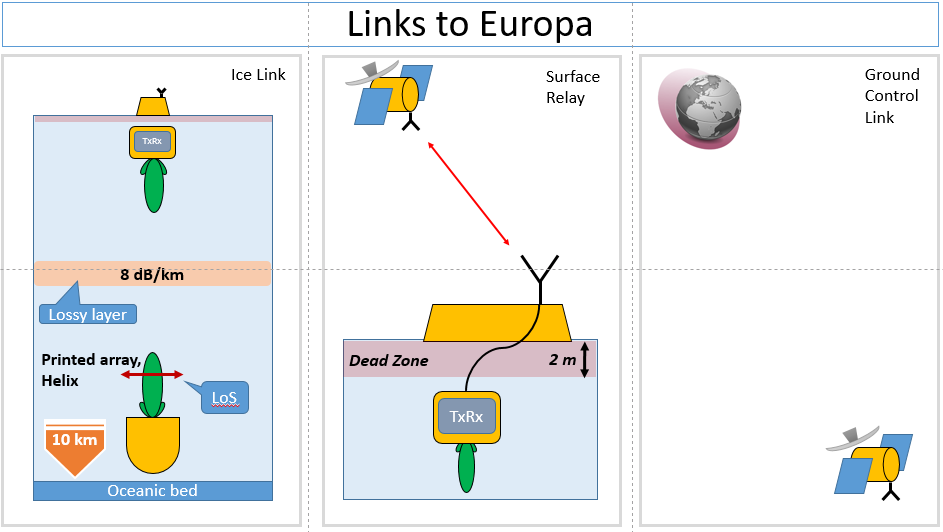
\includegraphics[width=\textwidth]{figures/comms/europaLinks}
	\caption{ \textit{DRAFT} Depiction of the three main stages of a mission to Europa from a telecommunications perspective.}
	\label{fig:europaLinks}
\end{figure}
%\fi

The interplanetary link is feasible thanks to the development of deep space communication networks by ESA (ESTRACK) and NASA (DSN), increasing the reliability of communications and navigation of spacecrafts on missions beyond Earth's orbit. This makes the main hazard during this phase, the high radiation environment of interplanetary space which requires designing for single fault tolerance, a redundant transponder system would be the must straight forward approach. Other problem for this mission stage is the pointing of the antennas since the higher gains needed, increase the requirements for the attitude control systems to keep direct line of sight with ground tracking stations. Universal Space Transponders (UST) are available for down/up-link in UHF with proven capabilities from previous missions to Mars with the inclusion of a down/up-link at X-band and a Ka-band down-link (UHF is TRL-9 and X,Ka-band is TRL-4 according to \cite{clipper}). This leads to focus on the details of a link with a possible Europa orbiter and more important the communications through the ice crust between the penetrator and the lander.




\autsection{Orbiter}{Johannes Linde}
The Europa Reconnaissance Imaging System (ERIS) plays an important role in the first phases of the mission. During the early stages, the imaging system will be used to map the surface of Europa and provide the necessary data for selecting a suitable landing site for the lander and penetrator. At this point, it is expected to have one or more cameras on the orbiter, mapping the surface of Europa in both low and high resolution. The Imaging System will be located in the orbiter, performing its primary objectives during the early stages of the life finding mission mission and performing the secondary objectives after a successful landing on Europa.

\autsection{Lander}{Maja Tomicic}
The landing-module should be able to perform a soft pin-point landing on the desired landing spot. The landing procedure should be completely autonomous using real-time on-board data from relevant sensors that are carefully selected ensuring that they meet the requirements for the landing as well as being mass and power efficient. After landing, the primary goal is to get the payload out of the radiation environment, therefore the possibility of melting a preliminary hole in the ice and dropping the payload into it, is investigated.

\section{Penetrator}
\autsubsection{Drilling Methods}{Lukas Christensen}
In order to get through the ice sheet on Europa some sort of penetration method is needed. Various possible solutions must be identified, and each must be analyzed to determine its viability. Once a method has been selected it must be thoroughly investigated and estimates for the penetration time must be provided and validated as it will form the basis of the overall mission design.

\autsubsection{Instrument Suite}{Morten Lykke Hilligsøe}
The instrument suites purpose is to generate data from which the following questions (presented in prioritized order) can be answered:
\begin{enumerate}
    \item Does life currently exist on Europa?
    \item Has life previously existed on Europa?
    \item How well are the conditions of Europa suited for life?
    \item What are the general characteristics of Europa?
\end{enumerate}

The presented questions will obviously rely on our definition of life, but if extraterrestrial life is anything like on earth, indicators will include the basic building blocks of life, chemical requirements and products of life such as trace metals and gasses, complex biochemical molecules which won’t be synthesized by simple physical processes and various physical requirements such as energy and temperature. The situation therefore requires several instruments to analyze the chemical, biochemical and physical composition, as well as a system for sample extraction and handling.

The problem definition at hand is then to make sure that if any form of life is present, the instrument suite will deliver the best possible data for detection and registration of this life. This kind of detection and analysis is constantly performed on earth, but a space mission to the subsurface sea of Europa places hard restrictions on the weight, volume, power consumption, durability and autonomy of such instruments. Therefore the optimal combination of instruments must be found, which support each other in the detection of life, while simultaneously complying with the restrictions at hand. 

As the surface of Europa presents an extremely hostile environment of vacuum, low temperatures and high radiation levels, answers to the questions presented are only sought after below the icy surface. Not only because life is not expected to be observed at the surface, but also because this will impose huge restrictions on the type of equipment capable of surviving these conditions, as well as added complexity, weight and costs. Instead the instruments will be protected by the lander and penetrator until safely inside the European ice crust.


\chapter{Theory}


\section{Moon Characteristics} % JP, Yannis

\iffalse
* Rock core, water, ice

    * Why do we think so?
    
    * Geysers?
\fi 

\subsection{Radiation Environment} % Maja, "landing site guys", "orbiter guys"

%* Both for the orbiter and the lander

\subsection{Tidal Wave} % Lukas, KSL

\section{Ice characteristics} % Lukas, KSL, Rasmus


\subsection{Structural Profile}
The first space probe flybys took place in the early 1970s, and Europa quickly became one of the main focuses in the search for past or present extraterrestrial life-harbouring environments, within reachable distances. Already in the 1960's were it discovered from earth-based observations, that the surface of Europa was covered in solid ice, not much unlike other satellites located that deep in the cold reaches of our solar-system. However, data recovered from satellite flybys supplied us with new information about the geology and composition of the moon's surface, having since helped us understanding the of Jupiter's, arguably, most interesting moons with respect to life-supporting environments.\\
\\
The Voayger mission from the late 1970's sent back coarse imagery of Europa with resolution in the ranges of kilometres per pixel, carrying valuable information about the surface of the Jovian satellite\cite{VoyagImg}. More specifically, the images showed a surface resembling that of a ball of string, discarding theories of Europa having a smooth surface, with it in stead being full of bands and ridges.\\%See requested article from DTU Findit
The Galileo spacecraft was launched in 1989 and entered orbit around Jupiter in 1995. It started transmitting data back to earth, from its extensive remote-sensing instrument suite
\iffalse 
(seen on fig. \ref{fig:GalInst1} and \ref{fig:GalInst2})
\fi
 with resolution surpassing Voayger's images almost three orders of magnitude. 
\iffalse
\begin{figure}[htb]
	\centering
	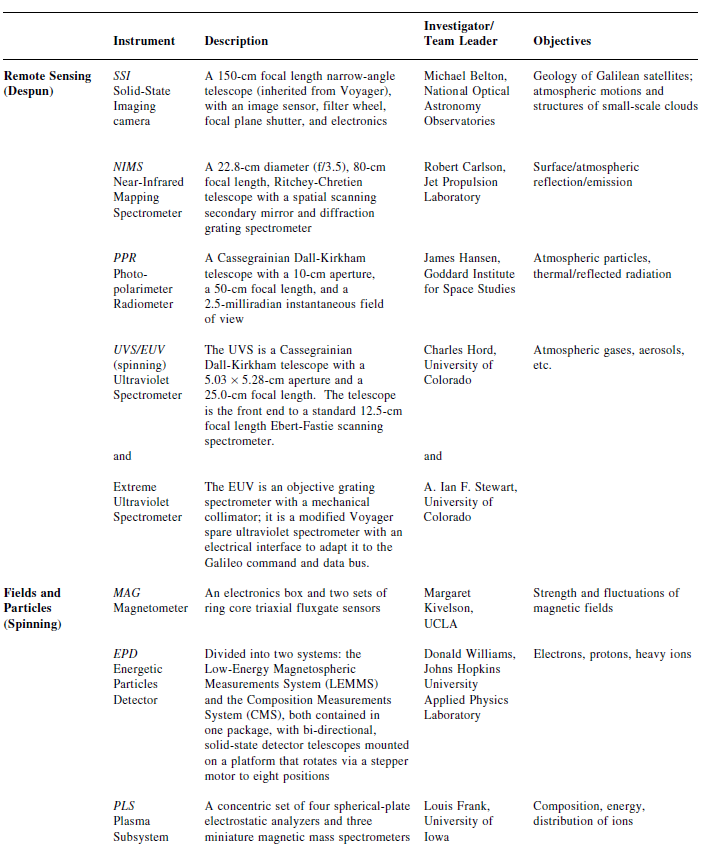
\includegraphics[width=\textwidth]{figures/Rasmus/GalileoInstrument1}
	\caption{Instrument suite of the 1989 Galileo mission.\cite{SciStrat} (\textit{Continued in fig. \ref{fig:GalInst2}}). \label{fig:GalInst1}}
\end{figure}
\begin{figure}[htb]
	\centering
	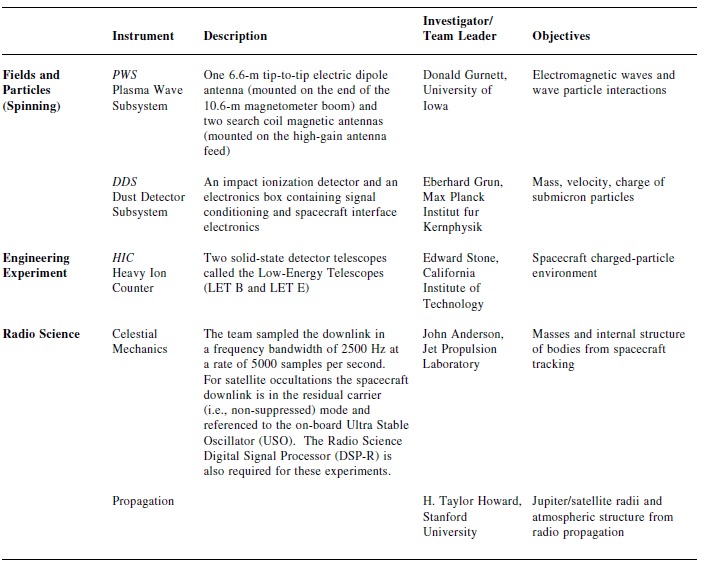
\includegraphics[width=\textwidth]{figures/Rasmus/GalileoInstrument2}
	\caption{Instrument suite of the 1989 Galileo mission.(Continued from fig. \ref{fig:GalInst1}) \cite{SciStrat} .\label{fig:GalInst2}}
\end{figure}
\fi
\\
The high-resolution measurements showed what seemed to be blocks of ice filled with ridges and/or early cracks, that had been lifted and rotated at some point in time. These disruptions indicates that there might be a liquid or softer slushy layer underneath the solid ice surface that through movement had broken and relocated the ice-crust. These cracks are illustrated on fig. \ref{fig:SurfCrack}, which is one picture of a series from the 1989 Galileo satellite\cite{HidOcean}. In any case, it indicates that there is some kind of structural activity in the outermost layer of the moon.\\
\\

\begin{figure}[htb]
	\centering
	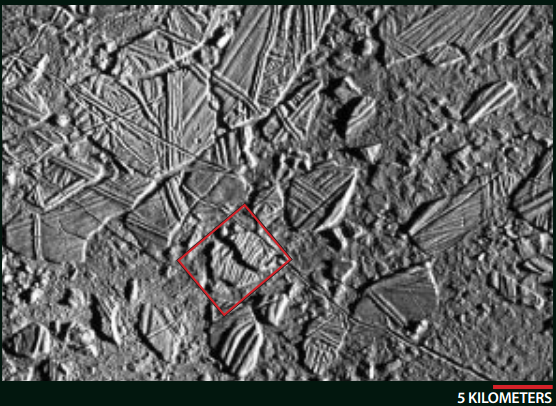
\includegraphics[width=\textwidth]{figures/Rasmus/SurfCrack}
	\caption{Image of Europa's surface taken by the Galileo satellite, showing ridges and disruptions in the surface. \label{fig:SurfCrack}\cite{HidOcean}}
\end{figure}

% Surface Composition
As explained in the study made by the Space Studies Board's Committee on Planetary and Lunar Exploration (COMPLEX), the data from Galileo’s Near-Infrared Mapping Spectrometer (NIMS) show that the water-ice absorption of Europa doesn't match with the expected outcome of pure-water ice, even for areas where the level of frozen sulfur oxide is thought to be lowest (The source of this $SO_2$ is presumably volcanic eruption on Io.). There has been some theories on the cause of this, including the presence of salts and other minerals in the ice but recent studies show that bubbles and fractions could result in the same discrepancies and band shifts in the measurements. However, it is still believed that some of the darker spots seen on the moon are observed because of salts and minerals like hexahedrite, epsomite, and natron\cite{SciStrat}. % INDSÆT The identity of that contaminant so far eludes scientists, but sulfur or iron compounds are suspected from Hidden Ocean P. 8
\\
\\
The actual thickness of the theorized ice-crust, and even the complete structural model of the moon, is still subject to many discussions. It was previously (prior to the Galileo mission) believed that the moon could be consisting of a hydrated silicate core coated in a thin layer of water-ice. However, with the measurements of Europa's gravitational field done by the Galileo satellite has this theory since been largely debunked. The current popular belief is that the cores is either a solid or fluid metallic core surrounded by a layer of water and ice of more than 100km due to the estimated density of the Jovian body. \\
The global ratio between liquid and solid water-ice is still unknown since it must be based on assumptions about the internal structure of the ice, which in themselves are extremely uncertain. The estimates we do have are even based on local imagery, since making them on a global basis requires dedicated orbiter mission, like the planned CLIPPER mission.\\%INDSÆT REFERENCE
In one study, the impact craters of Europa are analysed and compared with computer simulations to estimate regional crust thickness. The rationale is, that central peaks found in craters on the surface resemble material uplift caused by meteor impacts on extraterrestrial planets\cite{ThickImpact}, as seen on fig. \ref{fig:ImpactPic}. Therefore, it is assumed that the crust is thick enough to prevent complete surface penetration from meteor impact and as such they conclude that the ice at the impact sites must have been more than 	$\mathbf{3-4km}$ thick. Graphical representation of the simulation results can be seen on fig. \ref{fig:ImpactSim}. Another study that also investigated the impact craters, and taken from their introduction: "Stereo topographic profiles suggest that the plateau [a plateau SW of Cilix impact crater] is
flexurally supported, with an effective elastic thickness $t_e$ of
$~6km$. For a conductive temperature profile this $t_e$ value
implies a solid ice shell thickness of $\mathbf{~15km}$; if the shell is
convecting, this estimate is a lower bound. Combined with
independent estimates, we infer a probable shell thickness
of $\mathbf{25 km}$. The shell thickness is likely to be uniform over
the entire satellite."\cite{ThermElast}
\begin{figure}[htb]
	\centering
	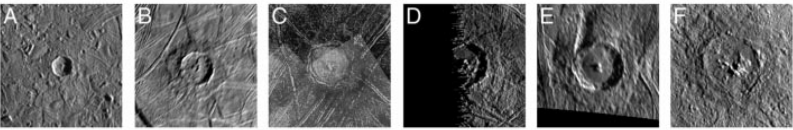
\includegraphics[width=\textwidth]{figures/Rasmus/Impacts}
	\caption{Galileo images of Europan central peak craters. (\textbf{A}) Brigid ($11^\circ$N, $80^\circ$W), $D=8.5km$. (\textbf{B}) Grainne ($60^\circ$S, $95^\circ$W), $D=13.5$km. (\textbf{C}) Cilix ($2.6^\circ$N, $182^\circ$W ), $D18.4$km. (\textbf{D}) Amergin ($14^\circ$S, $230^\circ$W), $D=18.6$km. (\textbf{E}) Maeve ($58^\circ$N, $75^\circ$W ), $D=20.4$km. (\textbf{F}) Pwyll ($25^\circ$S, $271^\circ$W), $D=23.7$ km. All images are at a resolution of 250 m/pixel and each is illuminated from the right except Cilix (\textbf{C}), which was observed at high sun
	\cite{ThickImpact}. D is crater diameter. \label{fig:ImpactPic}}
\end{figure}
\begin{figure}[htb]
	\centering
	\includegraphics[width=1\textwidth]{figures/Rasmus/Impacts2}
	\caption{Model results for impacts of large (A through C) and small projectiles (D through F) into 9-km-thick ice (gray) over liquid water (A) and (D), 5-kmthick ice (gray) over liquid water (black) (B) and (E), and 3-kmthick conductive lid (light gray) over convecting ice (dark gray) (C) and (F). Solid, dotted, and dashed lines show the regions of complete vaporization, complete melting, and $50\%$ melting, respectively.
	\cite{ThickImpact}.\label{fig:ImpactSim}}
\end{figure}
\\
Thermal models has also been used to estimate the average ice shell thickness of Europa. One study is carried out with the assumption of a ice shell decoupled from a silicate core by a layer of liquid water \cite{ThermThick}, so its conclusion may not fit with modern theories. They estimate the shell to have a thickness of $\mathbf{13-25km}$, depending on which thermal rheology model is used (Maxwell and general flow rheology, with and without heat flow from the core). Another thermal model is based on the suggestios of Europa having a metallic core and a silicate mantle, covered by significant layer of liquid water and a thinner ice shell \cite{ThermThick2}. The study heavily relies on convection in the ice, and this complicates the study further. The heat flow through the ice is dependant on the shell thickness, and shell thickness is in turn dependant on the heat flow. This study concludes on the result that the average thickness of a completely frozen shell must be around $\mathbf{36km}$ based on the study's assumptions.
\\
\\ One study carried out by [J.M. Wahr, M.T. Zuber et al., 2006] analyses the tidal effects caused by the differentiating gravitational pull from Jupiter, as Europa travels in its elliptical orbit around the planet. The result of the study is a set of analytical equations estimating the global thickness based on the Love-number of Europa. However, in order to utilize these equations, accurate knowledge of the ice-composition is required, as well as precise estimates of the Love numbers. In the end they even conclude conclude that their results may not be sufficient since they only provide an accuracy of $\pm 5\mathrm{km}$.\\
\\
Apart from the thickness and elemental composition of the ice, internal structure in the shelf is also highly relevant to the planned penetrator mission. Assuming a completely homogeneous ice-shelf is a crude over-simplification and may be a mission-killer if alternatives aren't considered. 
\begin{figure}[htb]
	\centering
	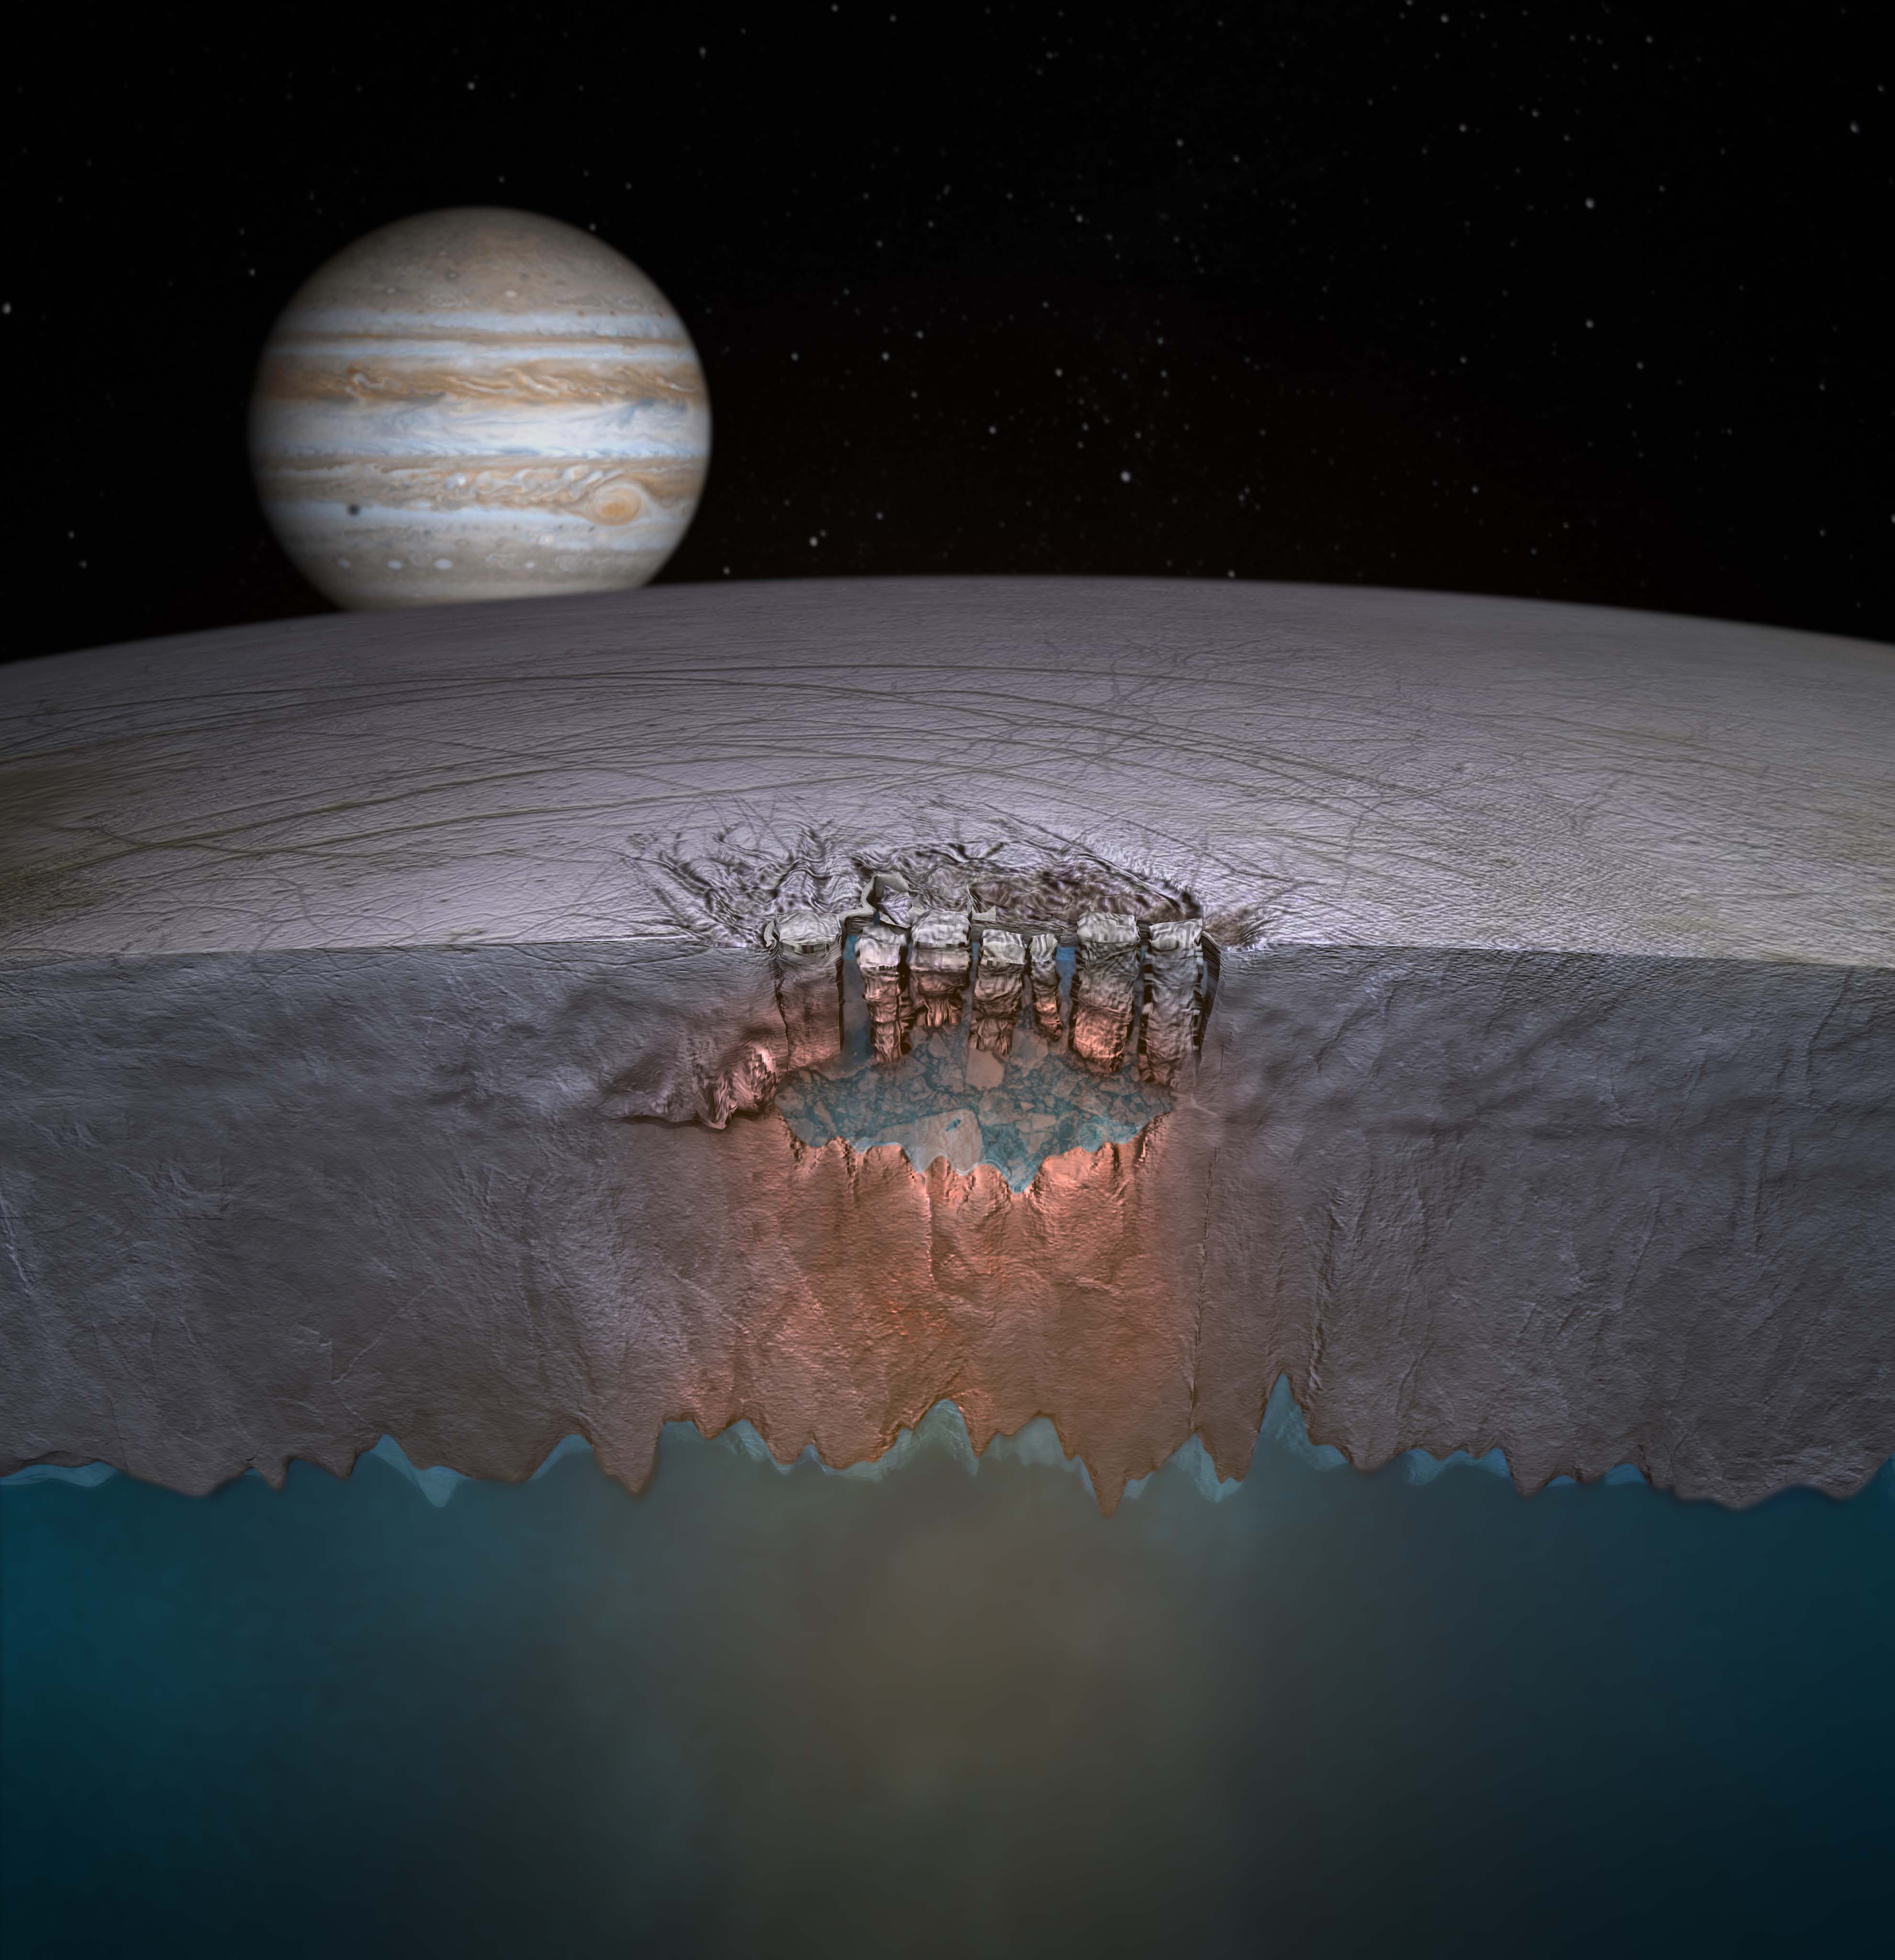
\includegraphics[width=0.5\textwidth]{figures/Rasmus/ArtLake}
	\caption{Artistic illustration of potential water lense, or lake, in the ice shell. \label{fig: ArtLake}}
\end{figure}
As such, apparent "Chaos Regions" has been observed on the surface of Europa and their causes has for a long time alluded scientists. However, recent studies suggests that these are formed due to water lenses in the shell, which can also be interpreted as lakes of liquid water \cite{IceLakes}. They way even be present within $3km$ of the surface, and it is estimated that there may be a water lense consisting of $20,000 - 60,000km^3$ of liquid water beneath the so-called Thera Macula chaos region. An artistic illustration of this phenomenon is shown on fig \ref{fig: ArtLake}.

\iffalse
* Ice thickness

* Composition of the ice? % Se: SWRI: "barr-showman-2009" (ask Kristian Lauszus)

* Lakes?
\fi

\subsection{Temperature Profile}

* "back of the envelope" calculations

\subsection{Pressure Profile}

* What is the outside pressure?

\subsection{Simulation Results}

\subsection{Simulation Validation}

* Should show that the "back of the envelope" calculations are right

\chapter{Defining Life}

One of the main objectives, if not the main objective, on this mission is to search for life. This is after all a life finding mission and therefore the instrument suite onboard needs to be focused on finding life. The mission is going to look for life in the ice and mostly in the water below the ice, where there is a high expectancy to find some sort of life or life harbouring conditions. \par
Life can be found in many forms and stages of evolution, and it can therefore be very difficult to detect, because we do not know exactly what the penetrator should look for. Before looking into what we should look for on Europa, a set of guide rules needs to be put in place, defining what life forms are already known from earth. It would be ideal to set up a precise yardstick for life, a list of things needed to say that life will exist, but this is not possible. What is possible is to look at what is present on Earth and applying this to alien life forms. \par
Most living organisms as we know from Earth have some properties in common, though non-living matter show some of them, only living organisms show all of them\footnote{$https://da.khanacademy.org/science/biology/intro-to-biology/what-is-biology/a/what-is-life$ 22-05-2016}. The 7 properties are: \par

\begin{enumerate}
  \item Organization
  \item Metabolism
  \item Homeostasis
  \item Growth
  \item Reproduction
  \item Response
  \item Evolution
\end{enumerate}

Beginning at number one “Organization”, to have life, structure is needed, and by taking unorganized matter and organizing it, is a sign of life. Living organisms a made up of one or more cells which in them self are highly organized, and able to produce complex chemical processes from an unorganized energy source. For bigger multi-cell organisms, organization is important, since individual cells are assigned different specific jobs to create a bigger and more complex organism. \par  
Metabolism is the life sustaining chemical transformations happening within cells and living organisms, and is the sum of all chemical reactions happening in a living organism. This chemical conversion can be divided into two subcategories, catabolism and anabolism. Catabolism is the process of breaking down organic matter into energy, with anabolism being the reverse process, building up complex molecules such as protein from simple molecules. This type of process uses energy. One of the most important metabolisms, is the citric acid cycle (Krebs cycle), it is believed to be one of the early established components for cellular metabolism. \par
Most living cells and organisms have a working area where they are able to sustain life; humans need to stay a cool 37 degrees to function normally. The ability to maintain a stable internal environment, even with a varying external environment is called homeostasis. This type of process is mostly found in more complex organisms, like smaller animals. Microorganisms usually depend on their surroundings to create a stable living environment.\par
The fourth properties is growth, this begins at a cellular level and is linked to the organization of the cells in defined structures. It depends on the anabolism to crate proteins and amino acids for DNA. Without growth more complex molecules and organisms would not exist.\par
Reproduction is also important for sustained life, looking at single cell organism like bacteria, which is able to reproduce by simply splitting in two. Reproduction can also take place with two parent organisms creating a new cell from a combination of both their genetic information. 
Organisms need to respond to actions from their environment to be able to survive. That is way many plants turn towards the sun, and bacteria cluster together around a nutrient rich area. When provoking a living organism, heating it, burning it, a response should be detected. It does not need to be movement, it could also be creating a toxin release or other chemical, helping it defend or survive from an unknown threat. \par
Lastly it needs to evolve, their genetics needs to adapt to changes, making it stronger and able to survive. Here natural selection is involved, where traits which make it easier to survive are carried through, by the death of the weaker organism that did not evolve. This is of cause a very slow process, but might be the key to discovering life on other planets, due to its adaptability.\par
These 7 properties of life are all found in living organisms on earth, this does not mean that the yard stick for life is defined perfectly, it is not! It is still hard to define life exact, and this only guides us some of the way. An example of where this does not hold true is for a mule, it is very much alive but is not able to reproduce\footnote{$https://en.wikipedia.org/wiki/Mule$ 22-05-2016}. \par
The properties can give an idea of what to look for when doing analysis of samples from Europa, because some of the processes create by-products that could be detected. One of the most well known processes with this ability is photosynthesis, taking CO2 and energy to create sugar and oxygen. It takes the suns energy and harvests it into chemical energy which can be used as fuel for the organisms. This type of process is very unlikely to take place in the ice or water of Europa, since the sun is 780 million kilometres away, and no light will get through the ice and down in the ocean. In general life needs to be rethought for the Europan environment.  \par
A good place to start the search for life is at the building block level, and looking for process that needs a source of energy, most likely heat, and some chemicals/nutrients, to create sustained life. This type of process is called abiogenesis\footnote{$https://en.wikipedia.org/wiki/Abiogenesis$ 22-05-2016} and is the natural process of living organisms arising from non living matter. The search could therefore go into look for simple non living matter such as simple organic compounds. This will narrow the search down to looking for molecules containing carbon, like in simple carbohydrates, this is of cause just one basic assumption for life, the other obvious one is the energy. No sunlight is reaching the ocean so energy must be created differently, by gravity or thermal activity in the rock core, this will be investigates further in the next chapters. \par
If the energy is there and some simple organic compounds can be found, life might be able to exist. The search therefore need to be increased to look for more complex molecules, here the organization property comes to play.  Now the search for proteins, and single celled organism, like bacteria would be possible living organisms.\par
This would go on, into bacteria colonies and even more complex organisms, but the conclusion is that we need some simple organic building blocks and energy to create some sort of life here on Earth (important distinction). Making a more generalized plan for what life is some other aspects needs to be taking into account by looking even further back to the origin of life.

\subsection{Hypotheses about the origin of life on Earth}
This is one of the difficult ones, because sciences do not know for sure how life came to be, but some important hypotheses have been made around where and how life on Earth originated from. \par
Life on Earth started some 3.5 billion years ago, the evidence for this is found in rock structures around the world, as small fossils of microbes. One place this is still evident today is in stromatolites which are produced by microbes by photosynthesis. They form a layer of microbial film, trapping mud under it, creating lay upon layer of mud and microbes, some dating back to 3.5 billion years ago. \par
The earliest signs of life are found on land, the main hypothesis to where life originates from is in the oceans, more specific the thermal vents on the deep sea ocean floor. The conditions found around these black smokers are ideal for an abiogenesis, due to the chemicals present and the energy in form of heat from the vents. DNA sequencing also suggest that some of the early life was microorganisms living in an aquatic high temperature environment. \par
As talked about in the previous chapter, life is complex, even on a microbe/bacteria level. These complex cells did not just show up, they evolved through small steps and natural selection. Hypotheses to how these more complex multi-celled organisms came to be can be split up in to 5 steps: \par

\begin{enumerate}
  \item In the beginning of Earth life, the atmosphere consisted of nitrogen, hydrogen, ammonia, water vapor and methane. This was able to combine in to simple organic matter, such as nucleotides found in RNA and DNA.
  
  \item The foundation was now set, and next came self replication molecules. These molecules are chains of nucleotides, and are able to replicate them self by some sort of RNA self-replicator process. With self-replicating came also natural selection, not all replications went well, and therefore some survive better than others. This process continued creating more and more stable and efficient replication processes.
  
  \item These replicating cells then got enclosed in a cell membrane, protection the self-replication molecules, these cells had a great advantages over the non enclosed cells, due to the protection of the internal environment from the outside environment.
  
  \item All of this was based on RNA-processes, but when some cells evolved to use DNA, things changed. Now instead of RNA doing the whole replication process, DNA became the genetic material, it is also more stabile then RNA, proteins became responsible for metabolism inside the cell and RNA now only did the part of carrying information from the DNA to the protein building areas of the cell. Below is a figure explaining the new replication process.

\begin{figure}[H]
\caption{The RNA is now the message carrier, and the DNA became the genetic material}
\centering
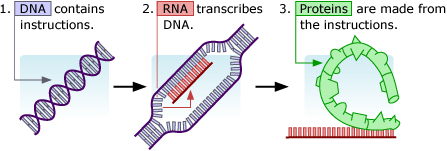
\includegraphics[scale=1]{figures/Agge/dnarnaprotein.png} 
\end{figure}
  
  \item Instead of the cells always splitting up after self replication, some stated to form more complex multi-celled organisms, the beginning of multi-cellular organisms.
\end{enumerate} \par

This was a short investigation into how life on earth could have evolved. Some of the hypotheses are still investigated and some gaps are still to be filled. An example of this is how RNA and proteins where created, because nucleic acids for DNA and RNA productions depend on proteins, but to build proteins nucleic acids are needed. The solution to this problem was first recently discovered, where the knowledge on RNA was expanded, and is was discovered that RNA is able to both store and copy itself concluding that nucleic acids came first \footnote{$http://evolution.berkeley.edu/evolibrary/article/side-0-0/origsoflife-01$24-05-2016}. \par

Many of these processes are dependent on energy from the sun, and it was after the first stromatolites and their photosynthesis the atmosphere started changing and became more oxygen rich. This will have worked as a toxic gas on some anaerobic cells, making aerobic cells more common on land. This just shows how many factors play a role on how life originated and further evolved, killing the first evidence of life as other life forms evolved.\par
From all of this a conclusion can be drawn in what might be expected to be found on Europa, a uplifting clue is found in the black smokers on Earth, which could be found on the bottom of Europa. But from what we see on earth, the most likely life forms are bacteria, or simple multi-cellular life forms, and what we need to look for includes, simple organic compounds, such as carbohydrates, enzymes, lipids fatty acids, nucleic acids, proteins, peptides, amino acids are some of the important compounds which could indicate life or a habitat for life.\par  
Another way to investigate life, is to look at the environment it is created from/in, and if life did exists we might see reminisce of life. The next two chapters look into the life harboring conditions and possible clues to look for from extinct life forms. \par

\subsection{Life harboring conditions and planetary habitability}
This chapter will look into the condition need for life to evolve on a planet, and since life beyond Earth is unknown, the theories on planetary habitability are built on what is known from Earth.\par
Planetary habitability, is a measure of a planet’s ability to harbour life in a habitable environment\footnote{$https://en.wikipedia.org/wiki/Planetary_habitability$ 24-05-2016}, this does not mean that life exists on the planet in question, but just that the conditions are right for life to develop, or to be transferred from another planet.\par 
Some of the requirement for life has already been discussed previously, but show up again in this chapter. One of them is energy, there need to be some sort of energy present, apart from that many other geophysical and astrophysical criteria must be just right, for a planet, to be habitable. Looking at one of NASA’s guide rules for life is “extend regions of liquid water\footnote{$http://www.nasa.gov/jpl/the-solar-system-and-beyond-is-awash-in-water$ 24-05-2016}”  since this is a great place for organic matter to form from, and here energy can come from either the sun in the top ocean layers, or for example black smokers on the bottom.\par
Habitability is not only dependent on the planets environment, atmosphere and so on, but also other externals needs to be considered; here we need to look at the astrophysical properties such as orbit and placement compared to the sun. In all there are many aspects to take in to account and like the chapter about “Defining life” some properties for habitability of a planet can be made:\par

\begin{enumerate}
\item Mass

\item Orbit and rotation

\item Geochemistry

\item Microenvironments and extremophiles

\end{enumerate} \par

The mass of a planet is important to sustaining an atmosphere; this is not a problem on Europa since the life is not expected to be found in its thin atmosphere. With smaller planets the energy left over from creation is lost faster making the planet geologically dead, this is a problem, since life is so dependent on an energy source. In the case of Europa the mass is very little compared to Earth which might point to a geological dead planet, and the energy must therefore come from the ice or the gravitational pull of Jupiter. But this does not always hold true, look at Jupiter’s other moon Io, is geological active, and even with its little mass. This activity comes from the gravity pull from Jupiter. \par
In the orbit stability is key; a stable orbit gives stability to the environment on the planet. The speed of rotation and how elliptic the orbit is, influences the temperatures on the planet, here stable temperatures are favorable, so half the planet is not frozen half the year and boiled the next half year. Looking at Europa the problem is not that impotent, since if life is found, it is located in the water protected by the sounding ice. \par
The geochemistry tells if the fundamental building blocks are present to create the “food” for living organisms. The four important elements from know from Earth are nitrogen, hydrogen, carbon and oxygen. It was already discussed in the chapter about life origin why these are important.  It is hard to tell if these are present in the ocean on Europa, a NASA study describe the “Why look at Europa” describes how hydrogen and oxygen might be present in just the right quantities.\par

When looking at a new planet maybe only a small part of it is habitable, comparing with Earth 3.5 billion years ago, life was not as abundant as it is now. Therefore a small sample from Earth would not have shown any sign of life, even if there was in some extreme place such as at the black smokers on the ocean floor. On Earth organisms know as extremophiles live in these very niche environments with conditions not suitable for “normal” life, there can be temperatures above 100 degrees Celsius, or very acidic/alkaline conditions. This expands the possibility of finding life in more extreme environments such as on Europa. \par
All of this can be summarized in a list of factors; the list was originally made for reproducing and survival of Earth microbes on Mars. The list has been modified to match an environment with no atmosphere\footnote{$http://mepag.jpl.nasa.gov/reports/MEPAG-SR-SAG-final1.pdf$ page 17 24-05-2016}.

\begin{itemize}
   \item  Water availability and activity
   \begin{itemize}
     \item  Activity of liquid water
     \item Past/further liquid (ice)
     \item Salinity and pH
    \end{itemize}
   \end{itemize}
   
     \begin{itemize}
       \item  Chemical environment
       
       \begin{itemize}
         \item Nutrients 
         
         \begin{itemize}
          \item C, H, N, O, P, S, essential metals and micronutrients
          \item Fixed nitrogen
          \item Their availability/mineralogy
         \end{itemize}
          
         \item Toxin
          \begin{itemize}
           \item Heavy metals (Zn, Ni, Cu, Cr, As, Cd, ect.
           \item Globally distributed oxidizing soils
          \end{itemize}
          
       \end{itemize}
     \end{itemize}
     
     \begin{itemize}
       \item  Energy for metabolisms 
       
       \begin{itemize}
         \item Solar/Radiation 
         \item Geochemical
         
         \begin{itemize}
          \item Oxidants
          \item Reductants
          \item Redox processes
         \end{itemize}
          
       \end{itemize}
     \end{itemize}
     
     \begin{itemize}
       \item  Physical condition 
       
       \begin{itemize}
         \item Temperature 
         \item Small temperature fluctuations
         \item High CO2 concentrations
         \item Water/ice flow
           
       \end{itemize}
     \end{itemize}
   
This list gives a good yard stick for determining if the planet is habitable, when Earth life forms are considered. Of cause life could be of a whole other unknown type which today’s technology cannot detect and this will give problems which is left out of this discussion. \par

\subsection{Extinct life}
Due to the small size of Europa, it might be geologically dead, but life might have thrived when the planet still had left over energy from its creation. Therefore it would be an idea to look for signs of extinct life, as we also see from Earth, previous life literally fuels today’s world. \par
When look for extinct life the search for distinct bio-makers/features that would indicate that life once thrived here. The things too look for will be leftovers from living organisms, this includes reduced carbon and nitrogen (CO3(2-), NO3-, NO2-, SO4(-2), also some important metals would be of interest Mg, Mn and Fe. But some of these compounds might not come from extinct life and it is therefore important to distinguish between biologically and not biologically produced compounds. An example of this is seen in the way N2 is deposited, with no biological processes the N2 would become NO2- and NO3-, but if this is used on a biological process it would form N2O or N2 as a gas  (dependent on pressure)\footnote{http://www.ncbi.nlm.nih.gov/pubmed/11537366 25-05-2016}. \par
From earth we see the extinct life in great quantizes such as olie and natural gas, produced by decomposing plants and animal matter under high heat and pressure. Natural gas is mainly made up of methane which would be a good marker for primordial life. Also olies floating on the water would indicate extinct life. \par

Through the last few chapters discussions about what life is and some of the signs to look out for have been investigated. Some of the findings have been applied to Europa and how it might fit the criteria as a life harbouring moon. In the last chapter a discussion about why Europa could be the place to go, for finding alien life in our solar system.\par

\subsection{Why look at Europa}

One of the most important properties of Europa is the liquid water found under the ice, which is key to life according to NASA, the more questionable, but just as important, is the energy need to create and sustain life. As discussed due to the small mass of Europa it might not be geologically active, if this is the case then a new NASA study carried out by JPL\footnote{$http://www.jpl.nasa.gov/news/news.php?feature=6514$ 25-05-2016} show that even without volcanic activity such as hydrothermal vents/black smokers, the balance of chemical energy might be there to support life. The study is based on methods know from Earth, and look at how energy and nutrients are carried around Earth’s oceans. But most importantly how the production of hydrogen and oxygen will take place without volcanic activity, one of the methods fro creating oxygen is serpentinization, where water reacts with freshly exposed rock (cracks form when cooling or water movement) to produce hydrogen. \par
The other part of the study looks in to the production of oxidants and oxygen, here the radiation from Jupiter splits ice/water on the surface, which cycles into the ice and down to the ocean. Scientist does believe that compounds from the top ice slowly cycles through the icy surface. If the amount of oxidants and hydrogen produced Europa is balnced just right, it might have just the right conditions to sustain life. \par
It is already know that Io has volcanic activity due to the Jupiter’s gravity push and pull on the rocky moon. This could indicate volcanic activity on Europa, giving even better conditions for life, due to the energy volcanic activity would bring. If Europa is geologically active there is a good chance of finding black smokers on the seafloor, this is one very important niche environment where life would thrive on the energy source and nutrients the black smokers produce.\par
Europa therefore seems like a perfect place to look for life and is also classified as a class III habitat. A planet in class III has liquid water of some sort trapped in or by ice, but since the water is enclosed the nutrient might be found in too small concentration to contain living organisms. This is the main problem with class III planet/moon, the lack of ingredients for life in one location due to the large water body and therefore lack of an incubator for life with the right amount of nutrients. \par
A illustration of all the possible methods for life to form is showed in the picture below, here radiation, ice cycle and volcanic activity would lead to a possible habitat for life in the ocean of Europa:\par

\begin{figure}[H]
\caption{The different process that Europa might have for producing a habitat for life}
\centering
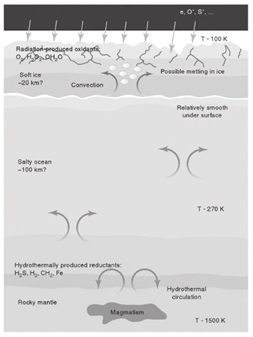
\includegraphics[scale=1]{figures/Agge/Europasurface.png} 
\end{figure}

In conclusion life is very complex to quantify and only a set of guidelines can be set up, derived from the life known to Earth. The guidelines set up give an indication of what to look for, when searching for a habitat or life on another planet, it also points to more precise investigations into what life forms might be found on Europa. It is still difficult to say anything exact of what could be expected to be found on Europa, in form of geology and energy source, but throughout this study it is evident that Europa is a good place the search for life in our solar system. In all Europa ticks many of the right boxes set up for a habitable moon with nutrition and energy to sustain life.


%* Water, oil, fat, carbon, energy
%
%* Proteins (amino acids) etc
%
%* Nutritions, water, heat energy
%
%* How can a life-form be able to convert thermal energy to other forms of energy
%
%* Another energy source could be geysers on the solid core
%
%    * A probe to the ocean bottom might show this
%    
%* Lakes inside the ice
%
%* Iron-reduction


\autchapter{Strawman Mission \& Instrument Configuration}{Paschalis Dalampiras}
% See awesome notes by "Johannes Linde"
\section{Strawman proposal}
\begin{figure}[htb!]
\centering
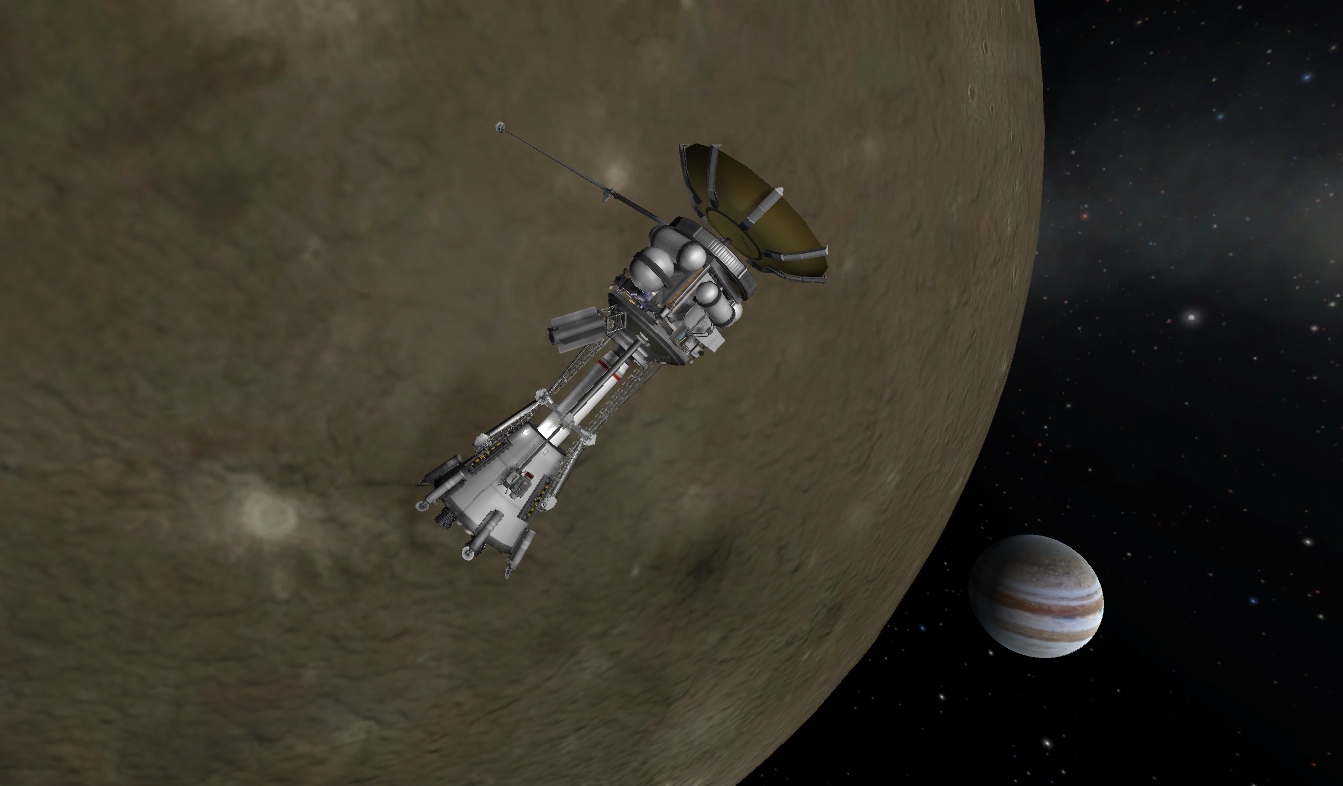
\includegraphics[width=\textwidth]{figures/Orbiter/9.PNG}
\caption{Spacecraft concept design, before orbiter-lander separation, performing a targeted encounter of Ganymede. (Kerbal Space Program)}
\label{fig:spacecraft}
\end{figure}

\newpage 
\subsection{Orbiter Concept}

\begin{figure}[htb!]
\centering
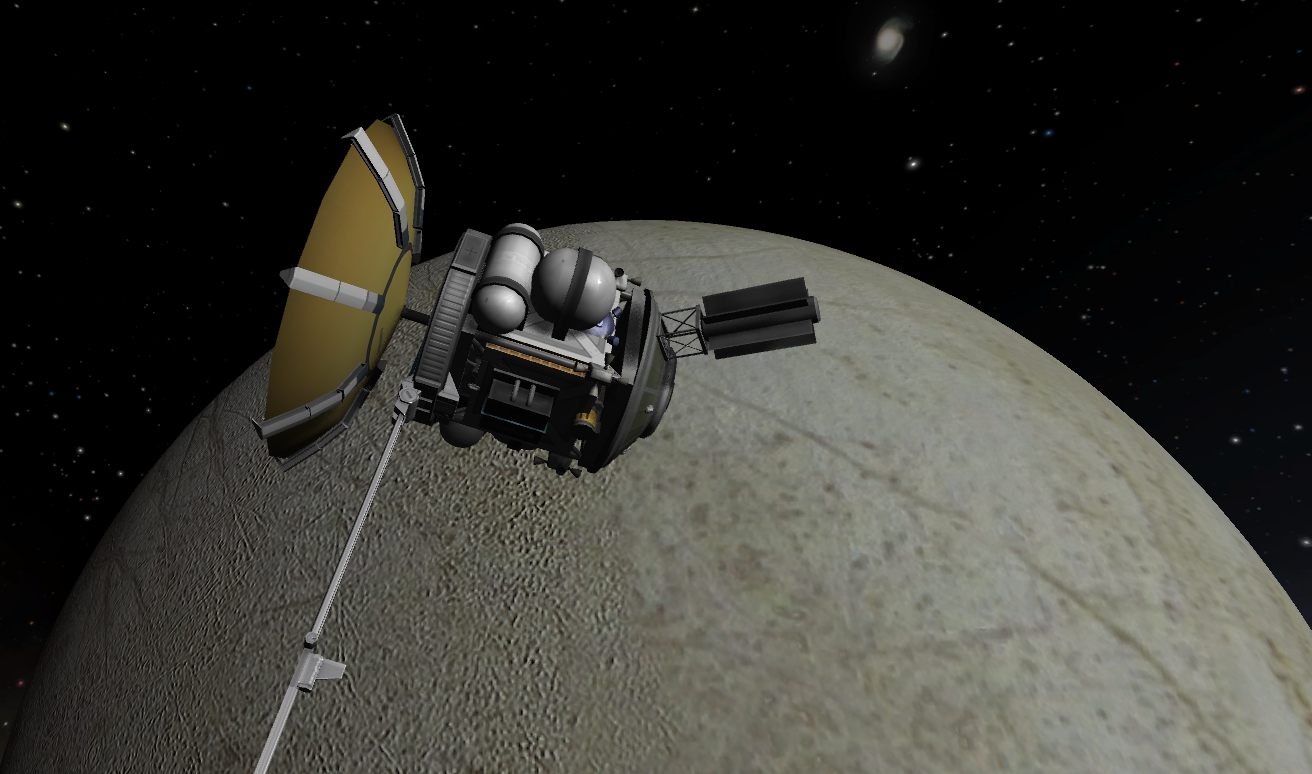
\includegraphics[width=\textwidth]{figures/Orbiter/orbiter.PNG}
\caption{Orbiter concept design, performing a flyby of Europa.(Kerbal Space Program)}
\label{fig:orbiter}
\end{figure}

\subsubsection{Orbiter Science}
Orbiter was designed to conduct a number of measurements to provide an insight into some of the geophysical characteristics that make Europa a unique environment of great scientific interest. Local topography of the moon’s volatile icy surface coupled with thickness measurements of the ice crust will expand the geological knowledge. Additionally, magnetic field measurements will reveal information of the induced magnetic field of Europa. As a secondary task, orbiter has also been assigned on collecting geophysical data of Ganymede and Calisto, taking advantage of the necessary flybys along these moons.

\subsubsection{Orbiter Mission Concept}
Conducting the planned measurements will require a set of remote sensing instruments (Optical spectroscopy camera, ground penetrating radar) as well as in situ instruments (Magnetometer) mounted on radiation shielded spacecraft capable of enduring the high radiation environment. Measurements will be carried out from varying altitudes ranging from 500km to 100km depending on the orbit sequence, providing local high resolution mapping of surface locations with high interest and investigating Europa’s magnetic field. 

\subsubsection{Orbiter Mission Design}
The spacecraft will be launched on a Delta IV Heavy rocket placing it into an interplanetary trajectory. A Gravity Assist Venus-Mars-Venus-Earth will guide the orbiter into a Jupiter Orbit Insertion after 3.7 years (Anastassios E. Petropoulos et al. 2000) where over the span of 165 days six gravity assist flybys of Ganymede and Europa will reduce the orbital delta v and place it into a highly elongated orbit around Jupiter. Performing a technique will set the orbiter in resonance orbit in respect to Europa. Orbit selection was based on the principal of avoiding long exposure over the area where radiation belts are more intense while on the same time allowing the craft to perform close flybys in resonance to Europa in order to complete the science observations.

\subsection{Lander Concept}

\begin{figure}[htb!]
    \centering
    \captionsetup[subfigure]{width=0.45\textwidth}
    \subfloat{
        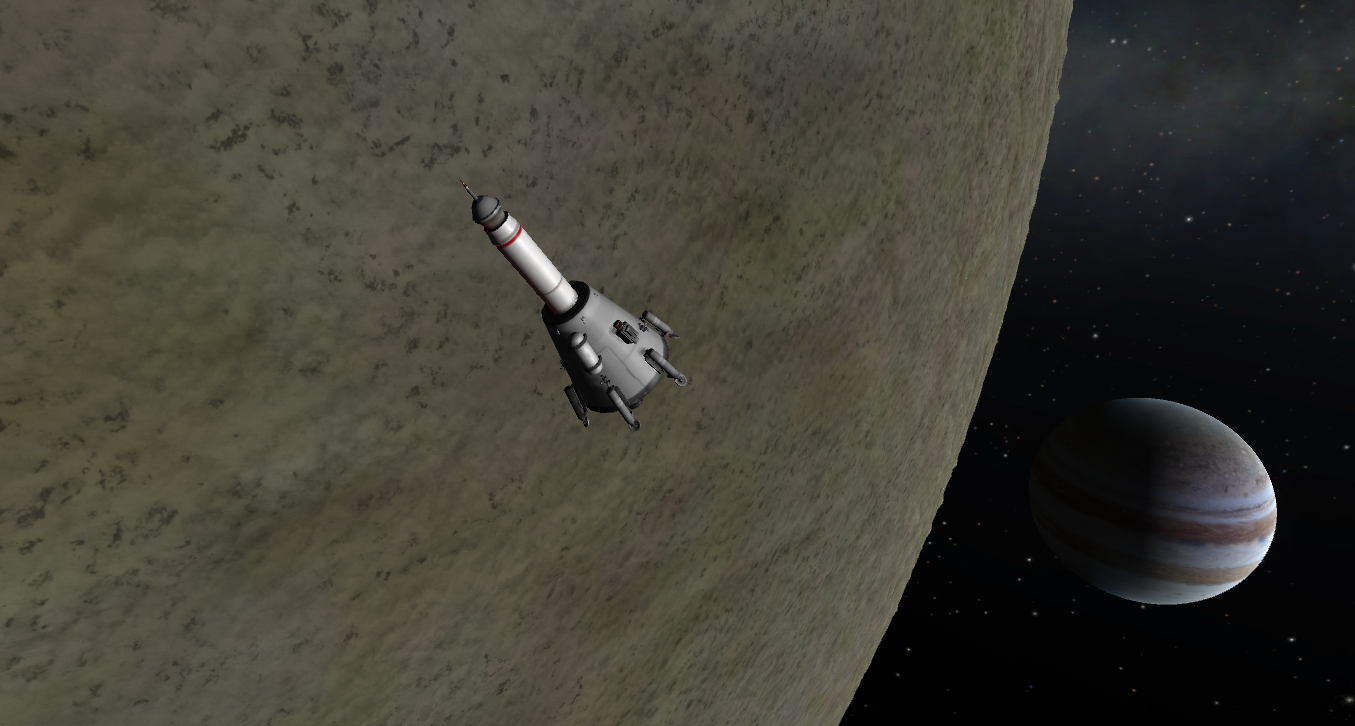
\includegraphics[width=.48\textwidth]{figures/Orbiter/2.PNG}
    }
    \subfloat{
        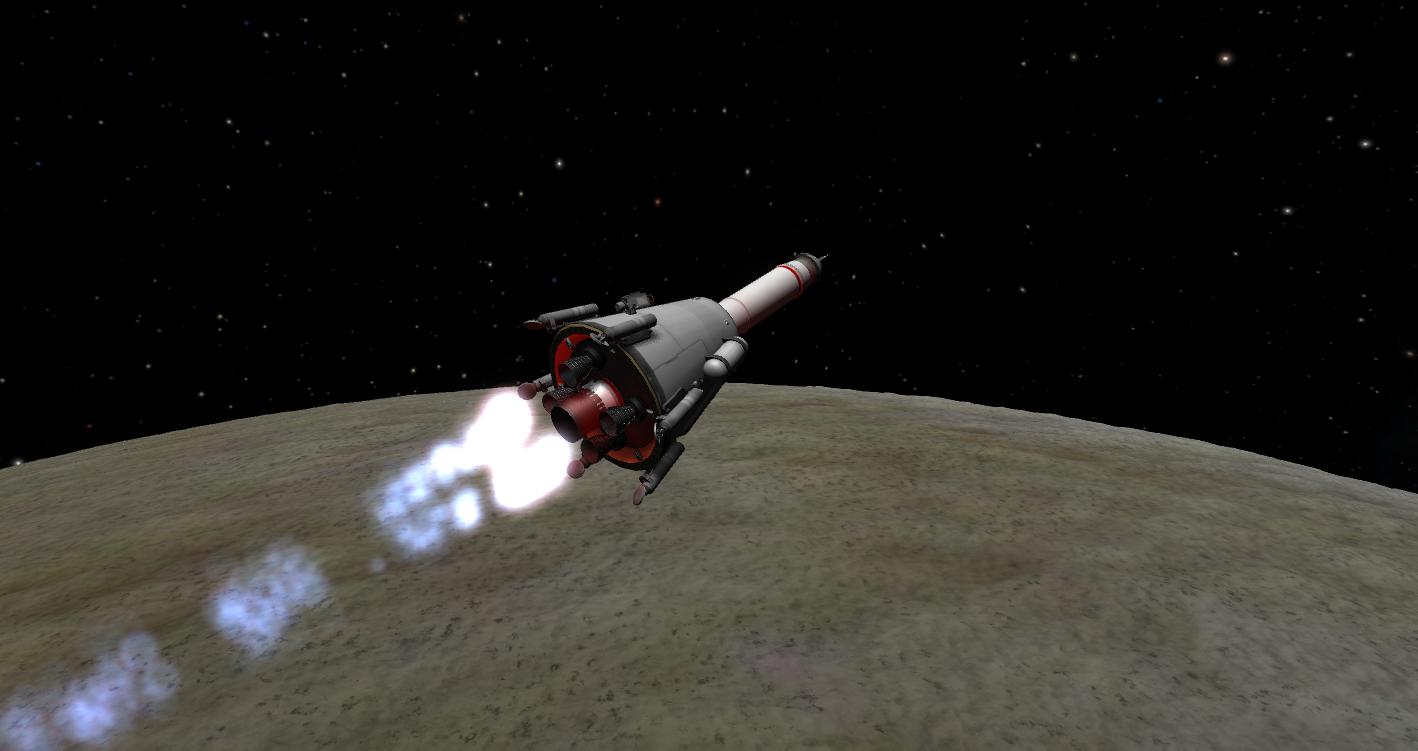
\includegraphics[width=.48\textwidth]{figures/Orbiter/4.PNG}
    }
    \caption{Lander concept design, preparing for descent.(Kerbal Space Program)}
\end{figure}

\subsubsection{Lander Science}

Main objective of the lander is to act as a secure and sufficient carrier of the designed penetrator, which will conduct a series of in situ experiments beneath the ice surface. Onboard surface cameras will provide high resolution images of the surface area and of the landing site, while microphones will record low amplitude sounds from potentially geological activity.

\subsubsection{Lander Mission Concept}
A highly radiation tolerant lander, capable of withstanding the blasting radiation in the near Jupiter environment will be deployed on the surface of Europa, delivering the penetrator safely and fulfilling the main goal of the mission. 
After acquiring data of topography and ice thickness measurements from the orbiter, a safe landing site will be manually selected after a reconnaissance campaign. A set of reconnaissance cameras will aid the landing while an angering system will secure the lander after landing, an essential system considering the low gravity environment of Europa. In order to facilitate the penetrator’s descent through the ice, main engines will be used to sublimate the top surface layer of the ice. Communication between orbiter-lander and lander-penetrator will be established using a set of two antennas with sufficient bandwidth for reliable telemetry.

\subsubsection{Lander Mission Design}

Lander will be launched attached to the carrier spacecraft, following the main trajectory sequence of the latter as described on the orbiter mission design.  
Release from the orbiter will be initiated at an altitude of 100km which will commence the descent phase. A micro-ASC unit is responsible for landing guidance, tracking the relative position of the lander. Two laser based devices, one for estimating the altitude range and one which will act as a structured light hazard avoidance system will assist the landing phase. An anchoring system will be deployed on touchdown, securing the lander from departing while a short burn of the main engines will use remaining fuel upon depletion to rapture the top layer of surface ice and prepare the conditions for the penetrator deployment. 

\subsection{Ice Penetrator Concept}

\begin{figure}[htb!]
\centering
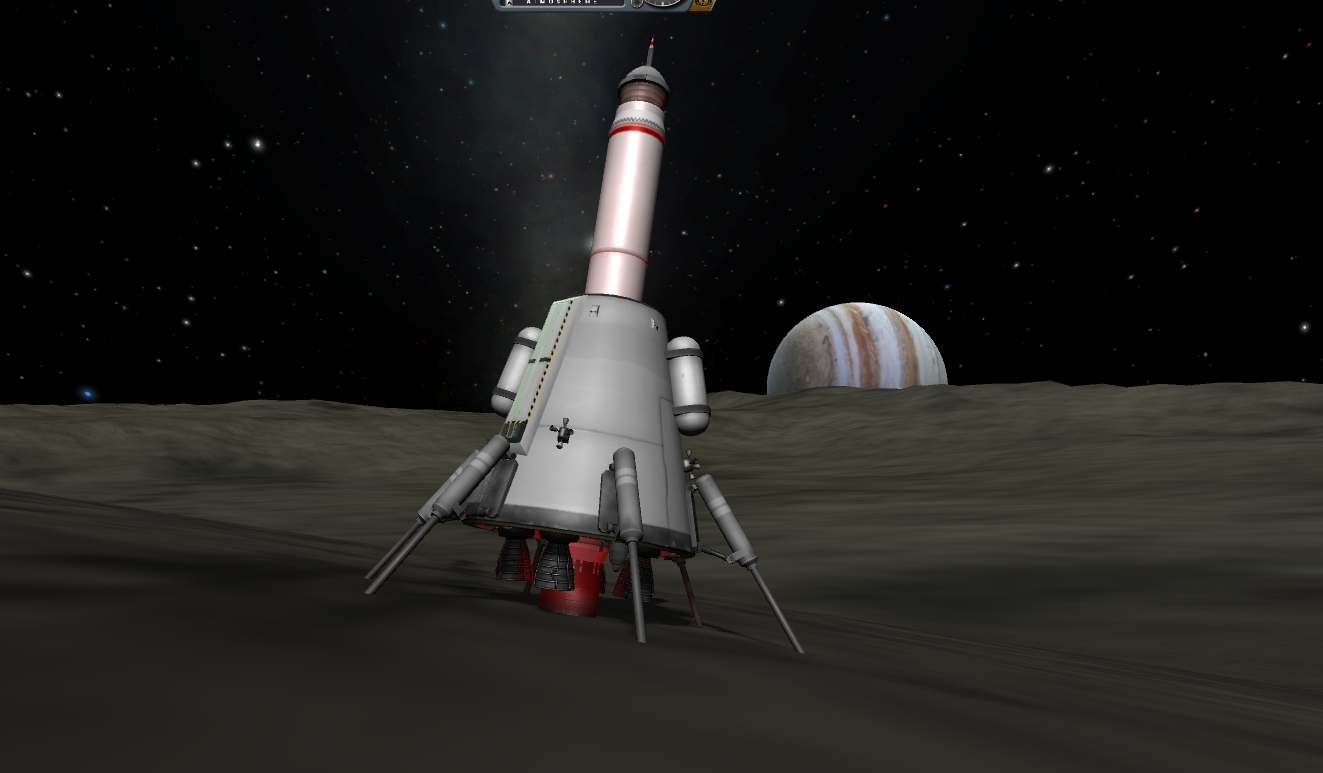
\includegraphics[width=\textwidth]{figures/Orbiter/8.PNG}
\caption{Lander with the penetrator deployed, preparing for the drilling phase. (Kerbal Space Program)}
\label{fig:penetrator}
\end{figure}

\subsubsection{Ice Penetrator Science}

Europa life finder mission concept relies on in-situ observations of the potential liquid water ocean beneath the icy surface of the moon. The highest priority objective of the mission is focused on detecting and analyzing potential life presence with the use of highly sophisticated and efficient scientific instruments. Secondary objectives include, investigation of the water composition by analyzing acquired samples as well as investigation of the ocean’s chemistry and characteristics of the water.
Science objectives are listed below.


\subsubsection{Ice Penetrator Mission Concept}

Measurements are carried out through a single location between the lower limit of the ice shell and the surface of the ocean. In-situ observations are conducted on the top layer of the ocean using a set of instruments deployed directly into the water.
Planned payload consists of nine instruments, a Mass Spectrometer, an Acoustic Doppler current profiler (ADCP), a Water Filtering System, a Microscopic Imager, a Barometer, a Thermometer, a Camera and a Microphone.

\subsubsection{Ice Penetrator Mission Design}

All the essential measurements will be conducted via a -torpedo shaped- self-propelled by gravity vehicle, capable of transferring and deploying the instruments beneath the floating icy shell that surrounds Europa. The ice crust is estimated to be several kilometers thick, thereat thermal power provided by an on-board Radioisotope Thermoelectric Generator (RTG) will be used to rupture and melt a 20-cm wide borehole through the ice, as the unit descents on higher depths. While descending, small size transceivers will be deployed and attached to the inner wall of the borehole in order to relay communications from the penetrator to the lander. Once penetrator has reached the surface of the under-ice ocean, an anchoring system will secure the vehicle on the ice and instruments will be deployed for the planned measurements. Acquired data will be relayed back to the orbiter through the transceivers and the lander’s communication system. 


\chapter{Orbital Mechanics}
%add list of todos to orbiter part
\newpage
\listoftodos
\newpage
%%%%%%%%%%%
%\autsection{Analysis}{Ifikratis Kamenidis, Paschalis Dalampiras, and Johannes Linde}
The Europa Life Finder Mission starts with launch from the Earth. The launch vehicle selection is based on the transfer orbit requirements and also available booster’s efficiency at the time of launch. At the time of writing (May 2016) the most powerful rocket that the mission can use is United Launch Alliance’s Delta IV Heavy. Thus, we are using this rocket for this mission. Since the mission’s wet payload is 5-6 tons, we make use of the VEGA (Venus Earth Gravity Assist) trajectory design. The design of this orbit depends greatly on the epoch of launch and for this study we use already published computations of alternative orbits. As we are interest in a 10 year time frame, we use a paper written by Anastassios E. Petropoulos et al\cite{petropoulos2000a}. In his work, the authors used the automated Satellite Tour Design Program (STOUR), provided by JPL (Jet Propulsion Laboratory) to examine 25 different sequences of gravity assists from Venus, Earth and Mars with low total $\Delta V$. For optimal solutions, the JPL Mission Design and Analysis Software (MIDAS) was used. The results of this study for low $\Delta V$ orbits from 2011 to 2013 can be seen in figure \ref{fig:grav_ass_traj}.

\begin{figure}[htb!]
\centering
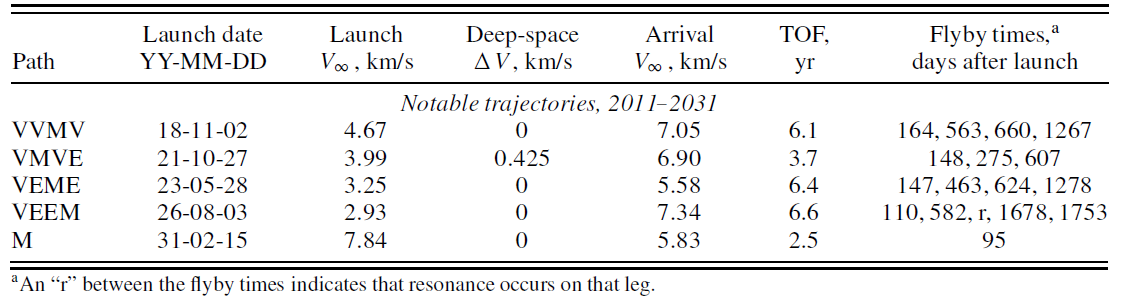
\includegraphics[width=1\textwidth]{figures/Orbiter/traj.png}
\caption{$\Delta V$ – optimized Jupiter gravity assisted trajectories from 2011 to 2031. \cite{petropoulos2000a}}\label{fig:grav_ass_traj}
\end{figure}

Selecting a favourable flyby path is a factor of minimizing cost and at the same time maximizing payload and time of flight (TOF) time. Also, reducing arrival hyperbolic speed ($V_{\infty}$) means less excess speed for the Jupiter orbiter insertion burn to take out and so less fuel needed for the burn. As we can see from figure 3.1, an opportunity of reaching Jupiter through Venus – Earth – Mars and Earth flybys, launching in May 28, 2023 will provide the least arrival excess speed while keeping the launch $V_{\infty}$ requirement low (Launch $V_{\infty}$=3.25Km/s). The VEGA orbit was used successfully by the latest Jupiter orbiter mission, Galileo as shown in figure 3.2.

\begin{figure}[htb!]
\centering
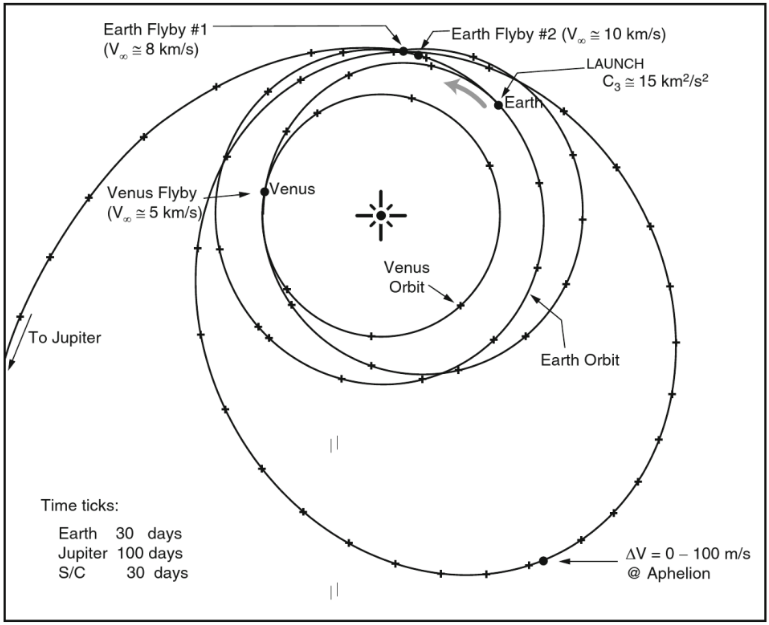
\includegraphics[width=0.8\textwidth]{figures/Orbiter/VEEGA.png}
\caption{The  VEGA orbit, used by the Galileo mission (Orbital Mechanics and Astrodynamics: Techniques and Tools for Space Missions, Gerald R. Hintz).}
\end{figure}
\section{Launch vehicle selection and evaluation}
To fulfill the mission trajectory requirement, the launch vehicle should be able to provide both the required energy and the payload capabilities of the Europa lander mission. We consided the case of two powerful launcher vehicles, the Atlas V 552 and Atlas IV Heavy by United Launch Alliance (ULA). The Atlas V family has shown solid reliability with 100 mission success since 2002 (United Launch Alliance, LLC), while providing the best match of payload mass and fairing sizes. The Atlas V 551 was used for the New Horizons mission to Pluto and Juno mission to Jupiter (one Earth flyby, TOF: 4.9 years), however the Europa lander mission will require a more massive payload to be delivered and so the Atlas V552 or even the currently more powerful rocket, the Atlas IV Heavy will be required. 

Using the required excess launch velocity of  $V_{\infty}$=3.25Km/s, we can calculate the characteristic $C_3$ energy which the rocket vehicle should provide to the payload that we want to arrive at Jupiter. This includes the full wet mass of the Europa lander mission (orbiter, lander, penetrator plus the required fuel for all phases of the mission). Using the Launch Vehicle Performance Calculator (Silverbird Astronautics \footnote{http://www.silverbirdastronautics.com/}) 
we calculate the maximum payload for an $C_3$ energy of $C_{3}=V_{\infty}^{2}=10.56 Km^2sec^{-2}$. Using the trajectory parameters from Table 3.1, the maximum payload for each rocket booster can be calculated and are shown in table \ref{tab:trajKg}.

% Table generated by Excel2LaTeX from sheet 'Sheet1'
\begin{table}[htb!]
  \centering
    \begin{tabular}{|c|r|r|r|r|r|}
    \multicolumn{6}{c}{\textbf{Maximum payload mass for the Atlas V 552 and Atlas IV Heavy boosters}} \bigstrut[b]\\
    \hline
    \textbf{Trajectory} & \multicolumn{1}{c|}{\textbf{Launch date}} & \multicolumn{1}{c|}{\textbf{TOF }} & $C_3(Km^{2}sec^{2})$ & \multicolumn{1}{c|}{\textbf{Atlas V }} & \multicolumn{1}{c|}{\textbf{Atlas IV}} \bigstrut[t]\\
    \textbf{} & \multicolumn{1}{c|}{\textbf{}} & \multicolumn{1}{c|}{\textbf{(years)}} & \multicolumn{1}{c|}{\textbf{}} & \multicolumn{1}{c|}{\textbf{552}} & \multicolumn{1}{c|}{\textbf{Heavy}} \bigstrut[b]\\
    \hline
    VMVE  & \multicolumn{1}{c|}{27-10-2021} & \multicolumn{1}{c|}{3.7} & \multicolumn{1}{c|}{15.9} & \multicolumn{1}{c|}{5181} & \multicolumn{1}{c|}{6759} \bigstrut\\
    \hline
    VEME  & \multicolumn{1}{c|}{28-05-2023} & \multicolumn{1}{c|}{6.4} & \multicolumn{1}{c|}{10.56} & \multicolumn{1}{c|}{\textbf{5648}} & \multicolumn{1}{c|}{\textbf{7389}} \bigstrut\\
    \hline
    VEEM  & \multicolumn{1}{c|}{3/8/2026} & \multicolumn{1}{c|}{6.6} & \multicolumn{1}{c|}{8.58} & \multicolumn{1}{c|}{5830} & \multicolumn{1}{c|}{7638} \bigstrut\\
    \hline
    \end{tabular}%
    \caption{Mass calculated in the 95\% confidence using Launch Vehicle Performance Calculator, Silverbird Astronautics.}
  \label{tab:trajKg}%
\end{table}%

\begin{figure}[htb!]
\centering
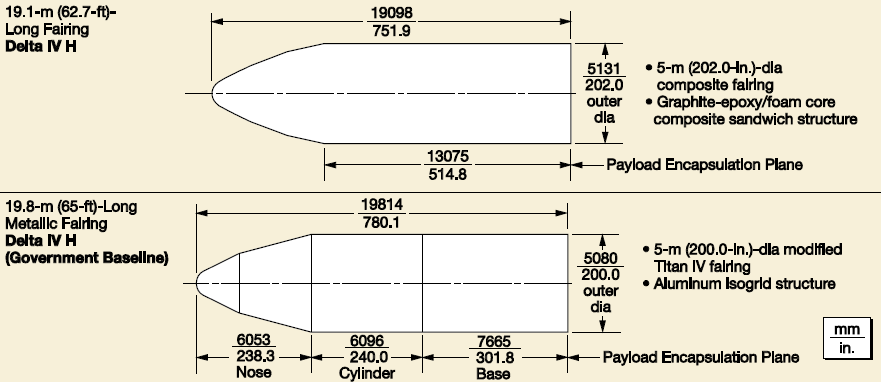
\includegraphics[width=0.8\textwidth]{figures/Orbiter/fairingsIV.png}
\caption{Atlas IV Heavy, fairing options dimentions \cite{Atlasm}.}
\end{figure}
\newpage
\subsection*{Payload dimensional considerations}
The physical dimensions of the spacecraft are limited by the launcher fairing options. The Atlas V and IV booster’s fairing options and a rocket's comparison view can be seen in figure \ref{fig:fairings}.
\begin{figure}[htb!]
    \centering
    \captionsetup[subfigure]{width=0.45\textwidth}
    \subfloat[United Launch Alliance fairing options (Delta IV Launch Services User‘s Guide, June 2013).\cite{Atlasm}]{
        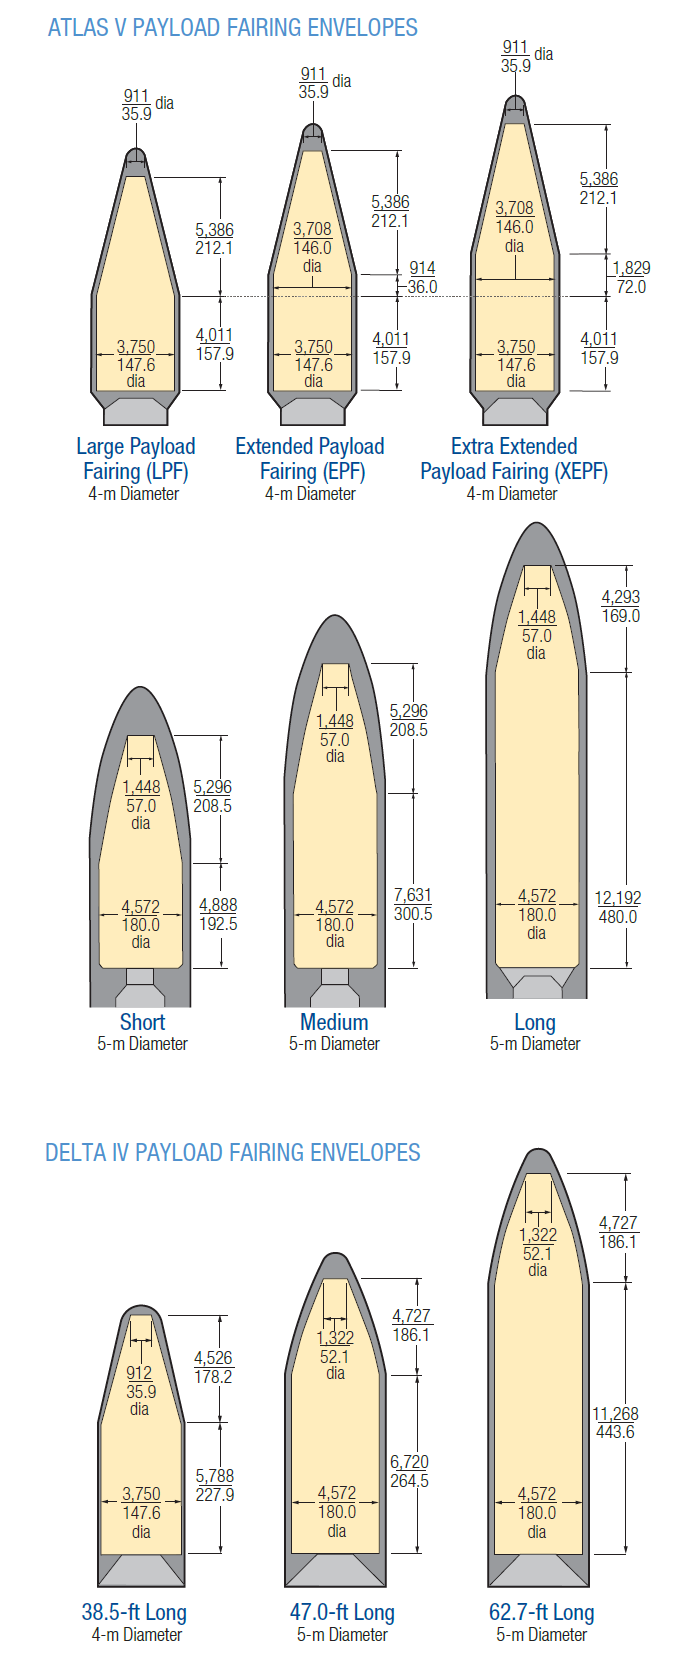
\includegraphics[width=0.48\textwidth]{figures/Orbiter/fairings.png}
        \label{fig:fairings_atlasiv}
    }
    \subfloat[Atlas V 552 and Atlas IV Heavy comparison (Delta IV Launch Services User‘s Guide, June 2013).\cite{Atlasm}]{
        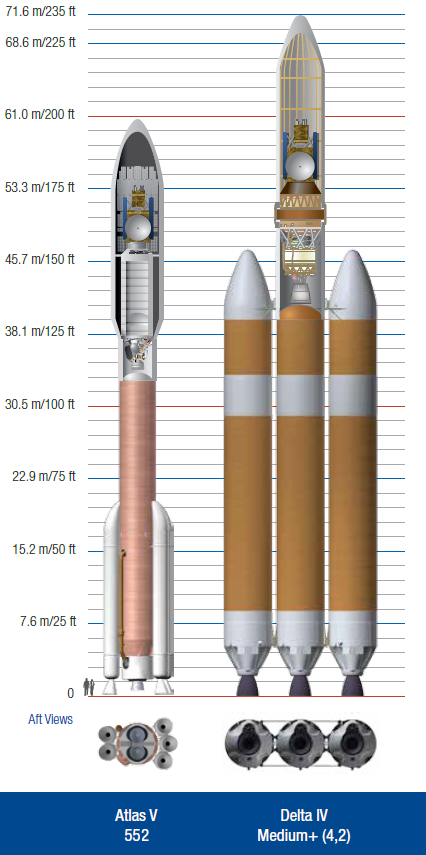
\includegraphics[width=0.48\textwidth]{figures/Orbiter/launchv.png}
        \label{fig:fairings_v_iv_compare}
    }
    \caption{Fairing Options}\label{fig:fairings}
\end{figure}
\section{Launch environment}
Launch is a mission critical event that requires significant attention for mission success. During launch, the spacecraft should survive in a fast changing and rough environment. From liftoff and until main engine cutoff (MECO), the engines produce a huge amount of mechanical vibration to the whole structure of the booster and so to the spacecraft which translates to a g-load on the delicate spacecraft components. 
Furthermore, the acoustic energy should also be considered. The acoustic environment is a function of structural design of both the fairing, fairing acoustic blankets and the spacecraft. The various components of the spacecraft should be assembled having in mind their oscillatory properties in the launch environment of the specific launcher. Another field of consideration should be the thermal properties of the ascent. As the launcher ascents the friction of the atmosphere molecules in the outer shell of the spacecraft fairing will significantly increase the fairing’s surface temperature. The acoustic blankets act also as a thermal insulator in the inner part of the fairing and so prevent the spacecraft of overheating. Further heating is avoided with fairing jettison which happens when the free stream drops below 1135 $W/m^2$\cite{Atlasm}.
Atmospheric depressurization inside the fairing is also a procedure that should be done in a controlled manner using an air duct valve. As the spacecraft may be required to wait in the launch pad in the case of an aborted liftoff, and during prelaunch activities, environmental monitoring is done using A/C and Gaseous Nitrogen($GN_2$). Temperature, relative humidity and cleanness are major concern, especially in a life seeking mission where the most demanding antibacterial protective measures are taken during the years of assembly prior to launch. Moreover, the Radioisotope Nuclear Generators (RTGs) will radiate heat continuously in the fairing enclosure and so temperature regulation is of paramount significance. Last, extra attention should be given to the outgassing properties of the fairing materials due to the intense heating that takes place during the ascent. Outgas molecules from nonmetallic materials can deposit on spacecraft materials and contaminate the sensitive life seeking instruments. 
According to ULA Atlas IV regulations, the acoustic blankets are made of Melamine foam covered with carbon-filled Kapton face sheets that eliminate outgassing and cleaned with isopropyl alcohol. The airflow during ascent should vent any outgassing molecules away from the spacecraft. However, elimination of non-metallic materials in the fairing to the lowest level is necessary. Graphical representations of the above parameters are shown in the following pages from the ULA Atlas IV user guide, version June 2013. Metallic fairing option is preferred for minimizing the outgassing factor. As it can be seen from figure \ref{fig:gloads}, the maximum load of the spacecraft will be approximately 5g at maximum dynamic pressure during first stage burn. Regarding the acoustic and shock levels, an acoustic and a vibration test is necessary to simulate and test the spacecraft rigidity prior to launch. The requirements for the acoustic test are shown in figure \ref{fig:testlevels}. The vibration test should simulate both launch vibrations and separation accelerations shown also in figure \ref{fig:testlevels} for various frequencies. Isostatic joints will be used to avoid stress forces on the spacecraft due to the temperature variations and differential thermal properties of the joint materials. 
\begin{figure}[htb!]
    \centering
    \captionsetup[subfigure]{width=0.45\textwidth}
    \subfloat[Delta IV Heavy (Metallic PLF) Absolute Pressure Envelope.\cite{Atlasm}]{
        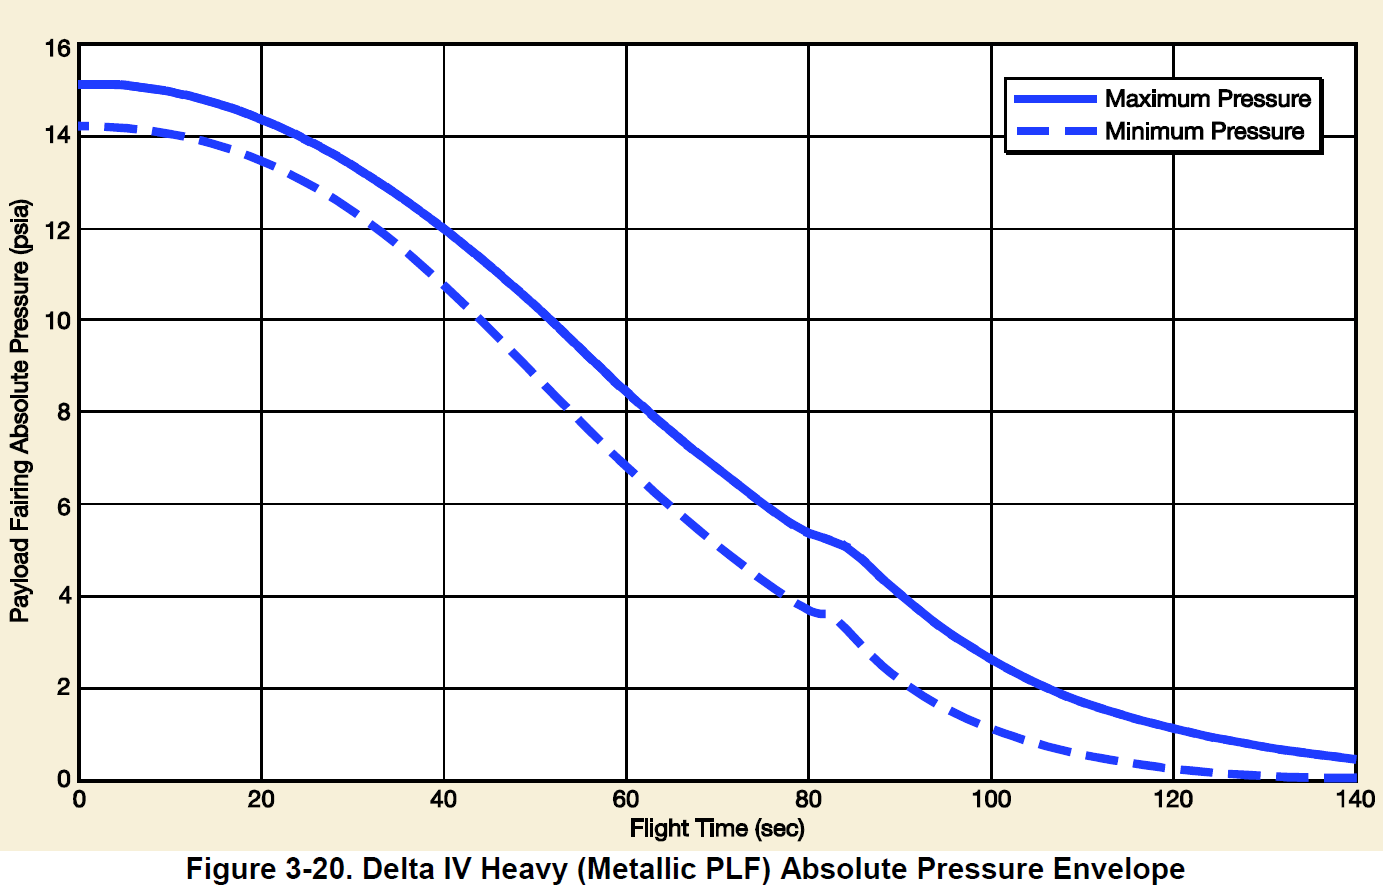
\includegraphics[width=0.48\textwidth]{figures/Orbiter/pressure.png}
        \label{fig:deltaiv_pressure_env}
    }
    \subfloat[Maximum Inner Surface Temperature - Environments to Spacecraft.\cite{Atlasm}]{
        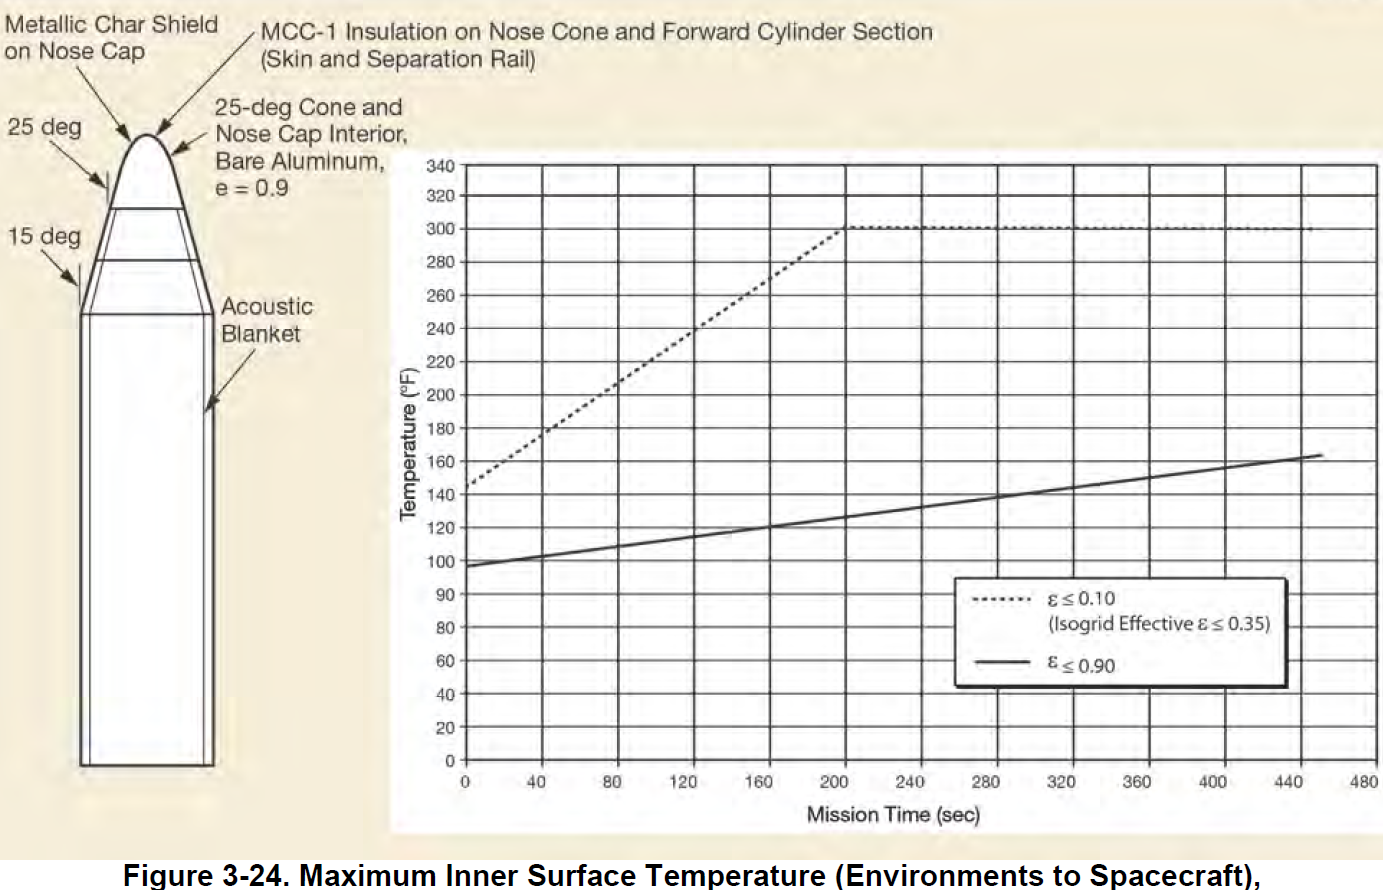
\includegraphics[width=0.48\textwidth]{figures/Orbiter/shell_temp.png}
        \label{fig:deltaiv_temp}
    }
    \caption{Pressure and temperature parameters.}\label{fig:press_temp}
\end{figure}

\begin{figure}[htb!]
    \centering
    \captionsetup[subfigure]{width=0.45\textwidth}
    \subfloat[First-Stage Burn vs. Second Stage.\cite{Atlasm}]{
        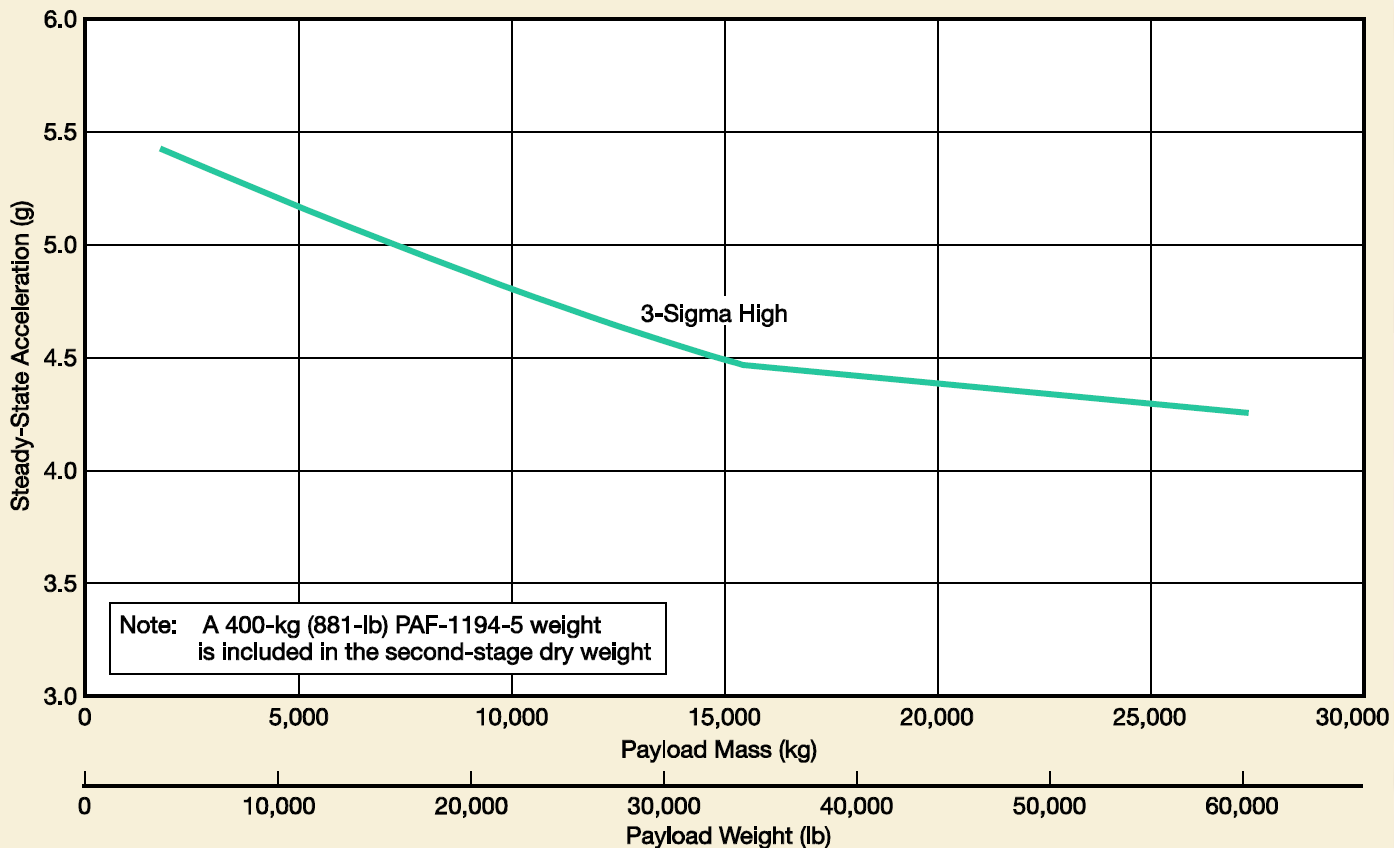
\includegraphics[width=0.48\textwidth]{figures/Orbiter/g_staging.png}
        \label{fig:gloads}
    }
    \subfloat[Second Stage Cutoff.\cite{Atlasm}]{
        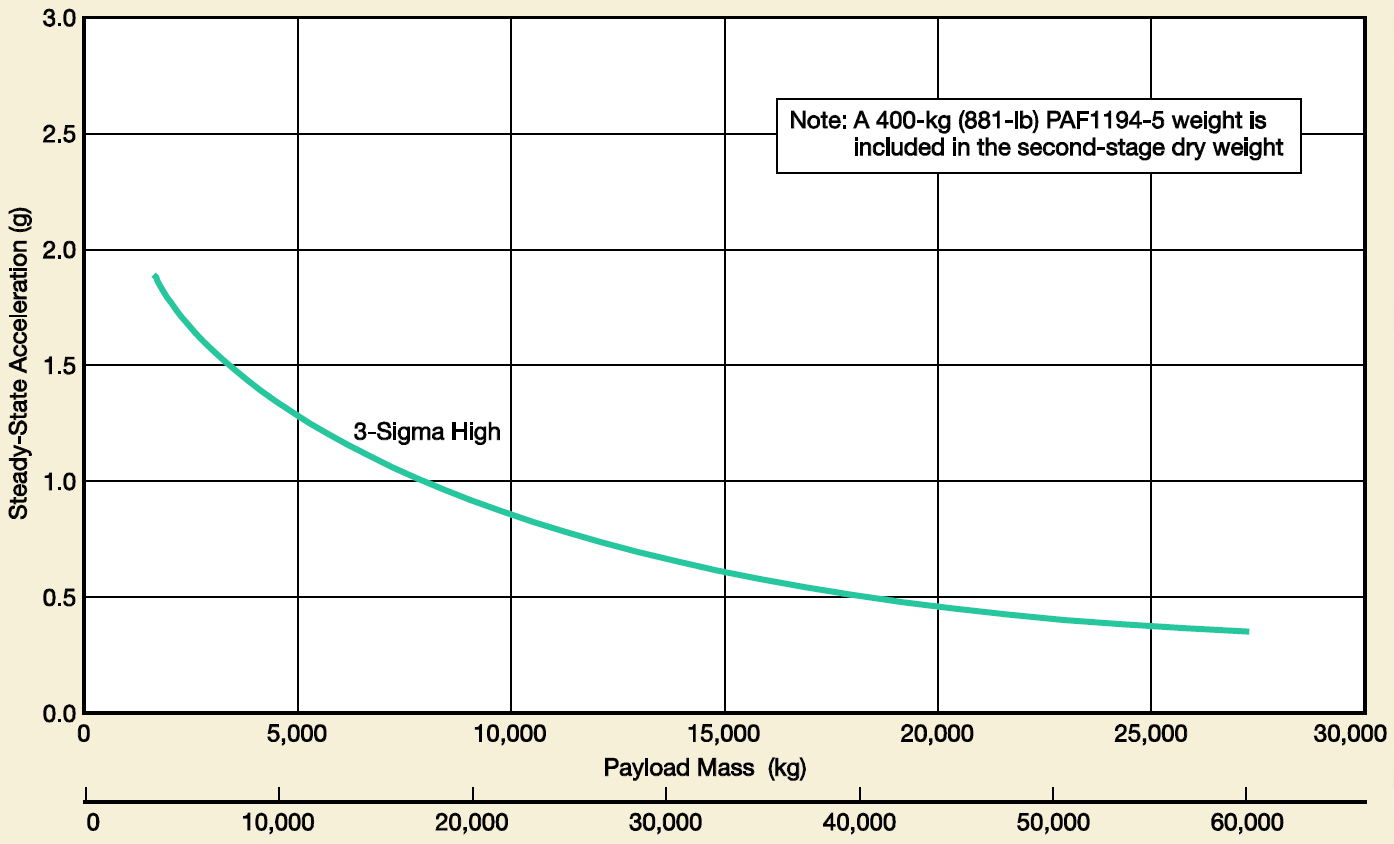
\includegraphics[width=0.48\textwidth]{figures/Orbiter/g_2ndstage.png}
        \label{fig:g_2ndstage}
    }
    \caption{Delta IV Heavy Maximum Axial Steady-State Acceleration}\label{fig:accel}
\end{figure}

\begin{figure}[htb!]
    \centering
    \captionsetup[subfigure]{width=0.45\textwidth}
    \subfloat[Maximum Spacecraft Separation Shock Level to Launch Vehicle.]{
        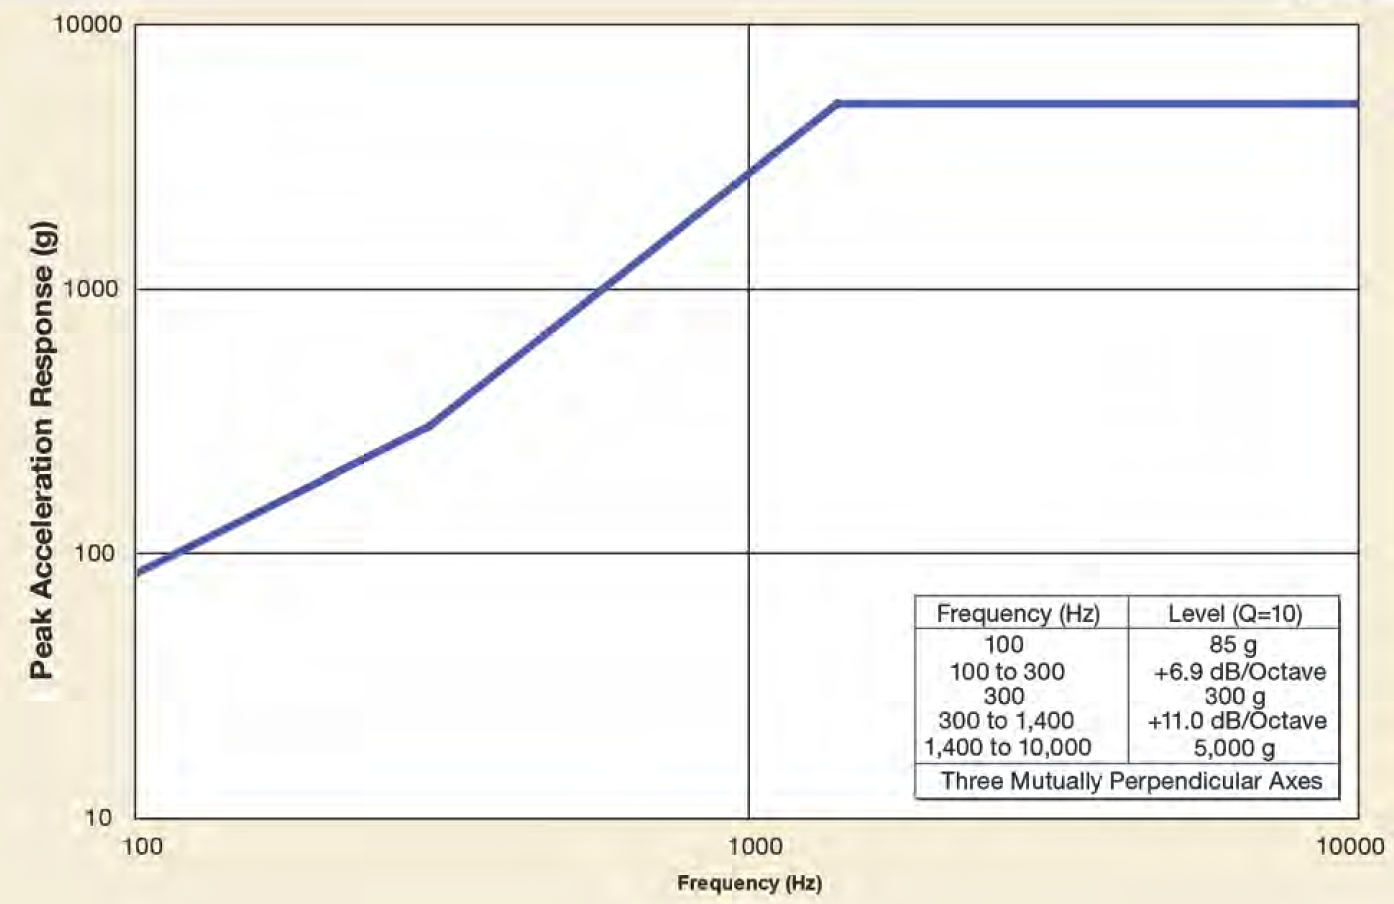
\includegraphics[width=0.48\textwidth]{figures/Orbiter/fairing_sep_resp.png}
        \label{fig:fairing_sep_resp}
    }
    \subfloat[Launch-Vehicle-Induced Payload Interface Shock Environment.]{
        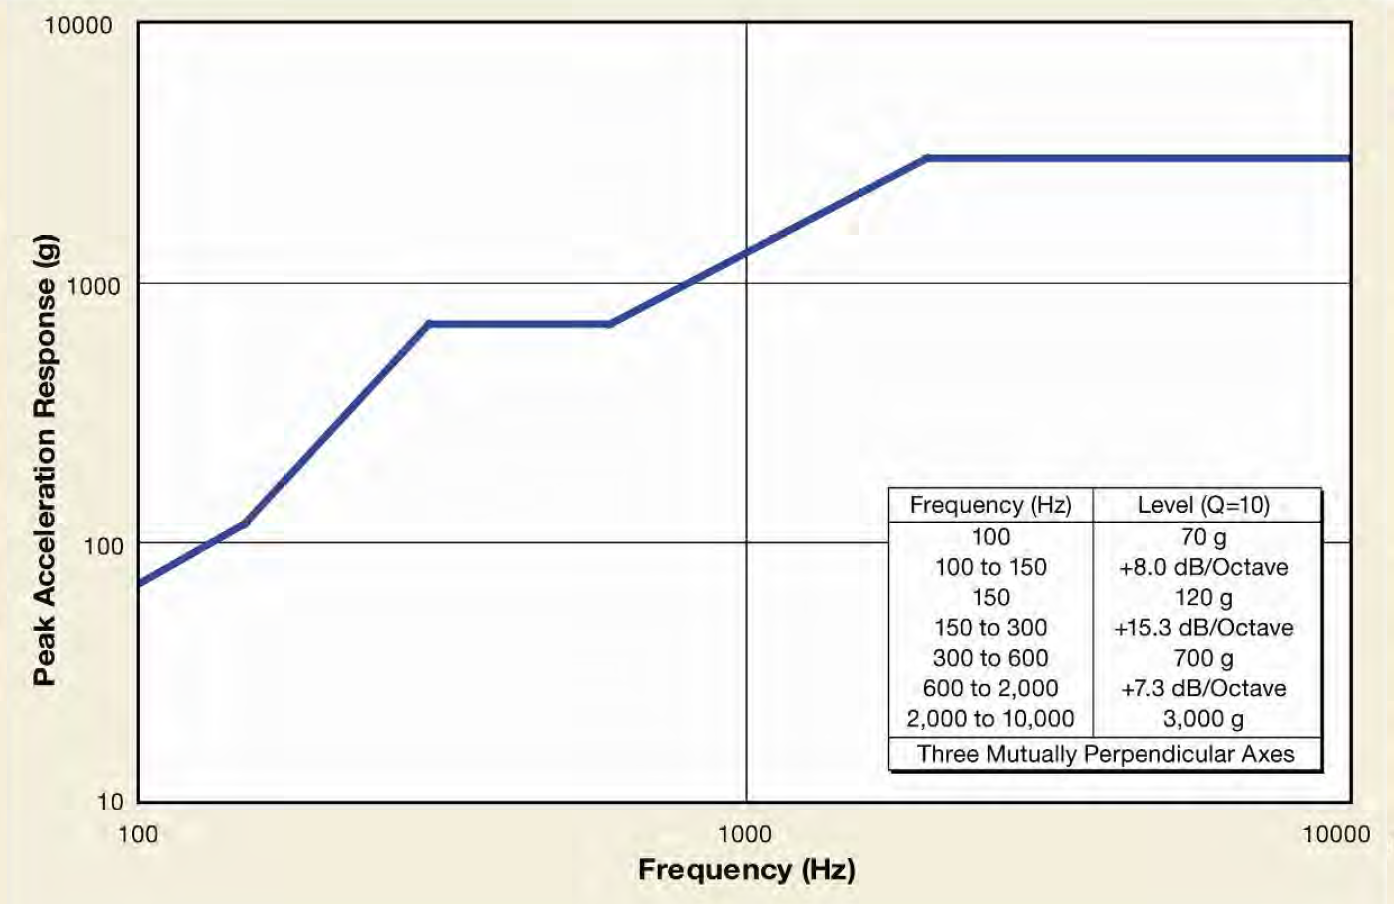
\includegraphics[width=0.48\textwidth]{figures/Orbiter/before_fair_sep.png}
        \label{fig:before_fair_sep}
    }
    \caption{Spacecraft shock environment. 1575-5 Payload Attach Fitting (95th Percentile, 50\% Confidence)\cite{Atlasm}}\label{fig:shock_env}
\end{figure}

\begin{figure}[htb!]
\centering
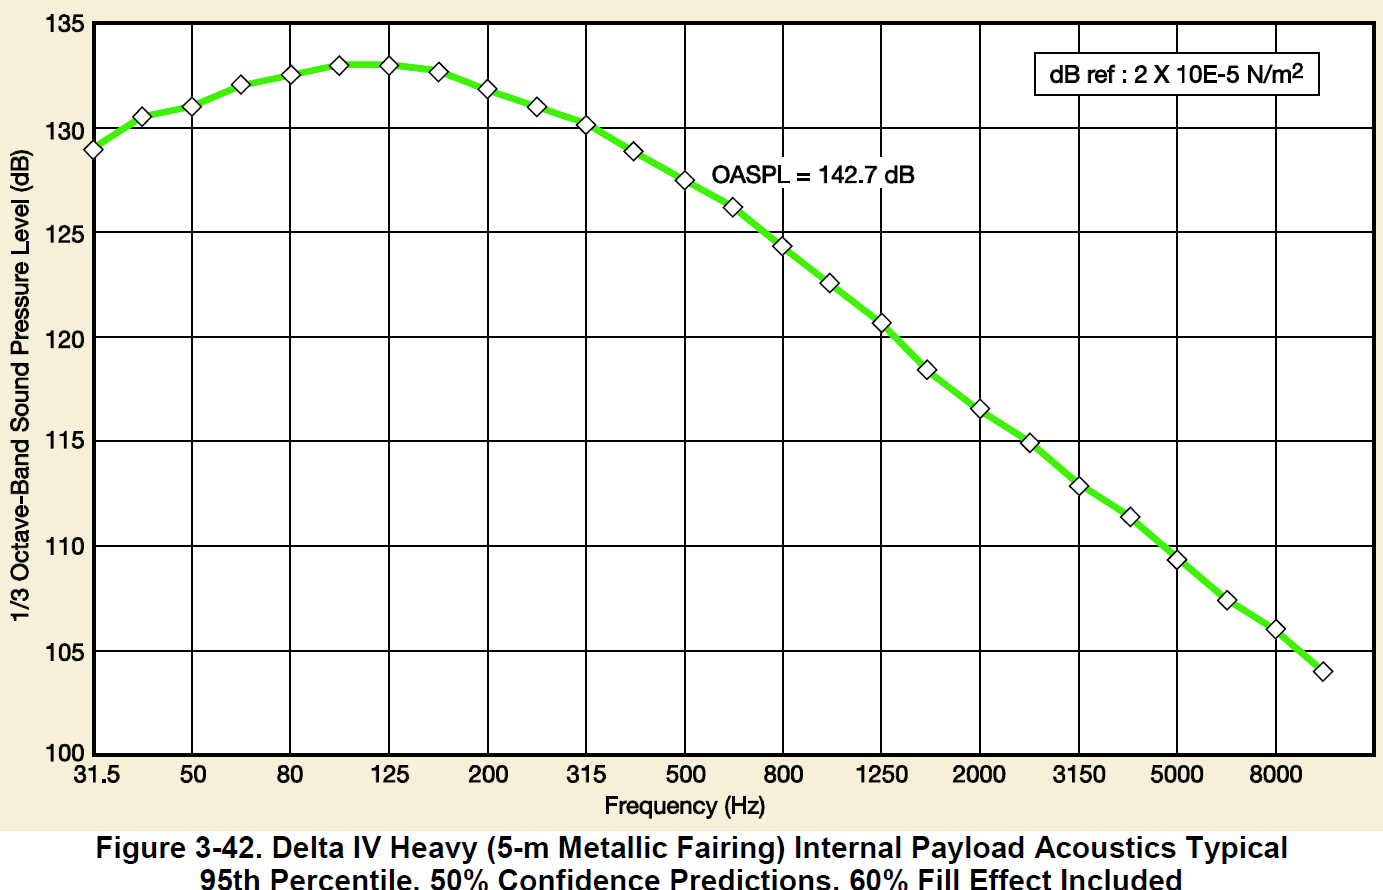
\includegraphics[scale=0.3]{figures/Orbiter/acoustics.png}
\caption{Delta IV Heavy (5-m Metallic Fairing) Internal Payl. Acoustics Typical 95th Percentile, 50\% Conf. Predictions, 60\% Fill Effect Included\cite{Atlasm}.}
\end{figure}

\begin{figure}[htb!]
\centering
\includegraphics[scale=0.3]{figures/Orbiter/acceptancelevels.png}
\caption{Acoustic and vibration test requirements\cite{Atlasm}.}
\label{fig:testlevels}
\end{figure}

\section{Cruise phase}
The cruise phase is the stage the spacecraft spends between launch and Jupiter arrival. During this 6.4 years period, the spacecraft should remain healthy and every system and science instrument should be designed to survive and be fully operational for the duration of its mission. 

During the cruise phase 4 flybys are planned, one from Venus, two from Earth and one from Mars. These flybys will provide the additional required $\Delta V$ to boost the apoapsis of the orbit to Jupiter's vicinity. The spacecraft will be equipped with a main engine and smaller Reaction Control System (RCS) thrusters. This propulsion system will be used to perform Trajectory Correction Maneuvres (TCM) to fine tune flyby trajectories. 

The flybys will also be used as a calibration test of the navigation and geolocalization system of the orbiter which will later be used to map Europa and find potential landing sites. As the mission is planning to flyby Europa multiple times when the Europa reconnaissance phase begins, the interplanetary flybys can be used as a useful analogy to simulate the flyby sequence and identify potential flaws before the actual mission begins. For example, small axis misalignment's of the telescope system with the star tracker’s axis can be spotted using star fields of both telescopic cameras and star trackers and so updating the rotational matrix parameters. This can be done by pointing to a known star fields. Precise knowledge of the spacecraft orientation is crucial for accurate pointing of the cameras while avoiding unintentional pointing of them to the Sun and at the same time keep pointing the high gain antenna to Earth.During cruise, all science instruments will be kept in hibernation mode to eliminate ageing degradation and potential software improvements found post launch will be addressed by software updates. Health checks of the systems will be performed many times during cruise. The cruise phase provides an additional benefit of using the telescope camera for Venus and Mars observations during the flybys as long as potential asteroid flybys on the way to Jupiter.

Special attention should be given to the thermal environment of the spacecraft during the flybys, due to the thermal heating of the inner planets which will be considerably more intense in the case of the Venus flyby. As the emitted energy is calculated using the black body radiation (given by Stefan-Boltzmann law)$L=4\pi R^2\sigma T^4$, where $\sigma$ is the Stefan-Boltzmann constant ($\sigma=5.670373\cdot 10^{-8}  Wm^{-2} K^{-4}$) and T the surface temperature and R the radius of the Sun. As the energy falls by the square of the distance from the source, it can be calculated that the highest solar energy the spacecraft will experience at Venus will be 1.9 times that of the Earth (or 2611 $W/m^2$ ). Given the extra heating from Venus high reflective atmosphere (albedo 0.90), \cite{venus_fact}, and the RTG constant heating, a shade solution should be implemented for the orbiter to keep the temperature to tolerable levels for both electronics and fuel tank temperatures. 

At a given time before Jupiter arrival (30-60 days), the high resolution camera will start an observational campaign of Jupiter’s satellites. The data will be used to update the orbital parameters of the moons and keep uncertainties of their speeds and positions to the lowest level for safety and fuel efficiency of the upcoming flybys and science mission trajectory. During cruise, the spacecraft will be using its high gain antenna pointing towards Earth, at the same time acting as a sun-shield. RTGs generated heat should be dissipated through radiators and carefully monitor fuel tank and temperatures distribution in the spacecraft.

\section{Jupiter orbit insertion phase}
After travelling for six and a half years in interplanetary space, the probe encounters Jupiter sphere of influence (48.2 million Km) (\ref{app:sphere_of_infl}). The Hofmann transfer orbit to Jupiter has provided enough energy so the apoapsis of the elliptical orbit will reach Jupiter at the same time that Jupiter is close enough to perform the JOI (Jupiter Orbit Insertion) burn. The telemetry commands for burn are expected to be sent to the spacecraft several days before closest approach. The inclination of the spacecraft incoming trajectory will be close to the Europa orbital plane which is $0.47^\circ$ to Jupiter’s moons plane and $1.79^\circ$ to the ecliptic (\footnote{Overview of Europa Facts". NASA}). That would be possible from the design of the flybys performed by the spacecraft. A number of small Trajectory Correction Maneuvers (TCM) are expected to be performed during the cruise phase to fine-tune the JOI timing and positioning parameters.

The JOI burn starts before closest approach to Jupiter, with the center of the burn happening exactly at the closest approach. Evenly distributing the timing of the burn is important for efficiently reducing the spacecraft’s orbital energy and being able to be capture into Jupiter's orbit. The spacecraft enters for the first time the magnetosphere of Jupiter at a distance of 45 to 100 $R_J$, which is the range of the subsolar point of Jupiter’s magnetopause (\footnote{The configuration of Jupiter's magnetosphere,Khurana, K.K.; Kivelson, M. G.; et al. (2004)}. and is affected by Solar activity. Arriving at solar maximum, the spacecraft will encounter the magnetosphere closer to Jupiter than in a low intensity solar wind period. The JOI burn will take place between the orbits of Europa and Ganymede as this configuration leaves open the possibility of using an initial Ganymede flyby to reduce the required delta-V for Jupiter orbit capture. At the same time, targeting a JOI burn close to Europa minimizes the requirements for a larger post orbit clean-up apoJove burn to bring the periJove of the orbit to Europa’s vicinity. Moreover, the periJove burn at this altitude avoids exposing the spacecraft to the high intensity Jovian radiation belts, the harshest region of them being within 300,000 Km from Jupiter\cite{jupiter_radiation_harsh}.

An analytical examination of the radiation environment is carried out in section \ref{sec:radiation_environment}, where SPENVIS models are used to predict the estimated doses from the high energy protons and electrons. Several minutes before the critical JOI burn take’s place, the spacecraft will re-orient itself for the retrograde burn and thus remain out of high-gain antenna contact with Earth during the duration of the burn (LOS). At that time, a smaller low gain antenna will be used to provide tone signals relaying vehicle status. 
\section{Jupiter Orbit Insertion delta-V calculation}
A limiting factor in the mission is the total payload that can be brought to Europa. Before that, the spacecraft should be captured in orbit around Jupiter. We investigate the amount of fuel such a maneuver will require, having in mind that the upper mass limit is defined by our launcher vehicle, which will be the Atlas IV Heavy with the maximum payload capability of 7389Kg as calculated in table \ref{tab:trajKg}.

The spacecraft arrives at Jupiter in a hyperbolic trajectory. Jupiter gravity becomes important at the sphere of influence radius of Jupiter \ref{app:sphere_of_infl}.
, which is around 48 million Km. The hyperbolic excess velocity can be expressed as the difference of the spacecraft trajectory at the apoapsis of its Hohmann transfer orbit $V_{SC,A}$ and Jupiter’s orbital speed $V_J$:
\begin{equation}
V_\infty=V_{SC,A}-V_J
\end{equation}

\begin{figure}[htb!]
\centering
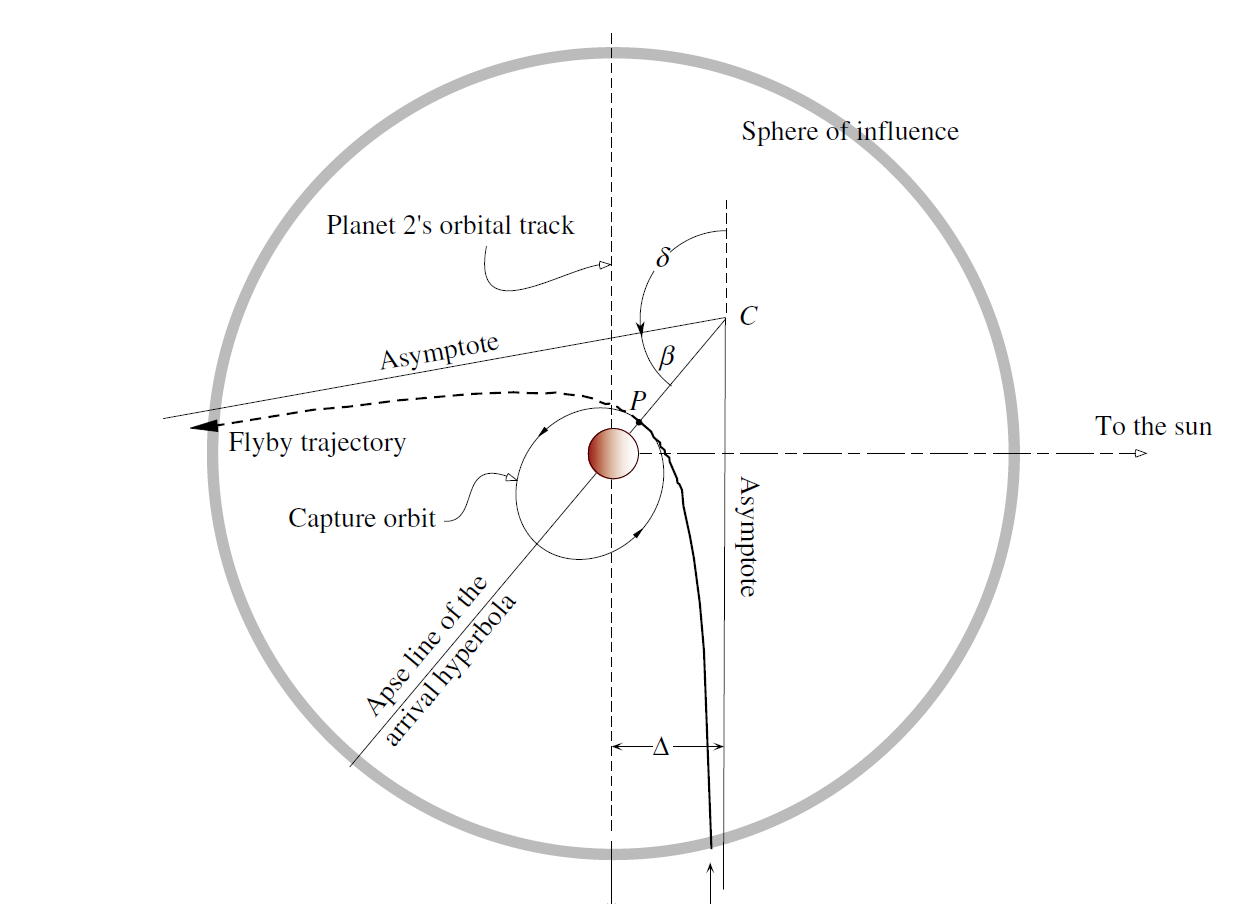
\includegraphics[scale=0.3]{figures/Orbiter/capture.png}
\caption{Incoming asymptote trajectory to Jupiter (Howard D. Curtis, Orbital Mechanics for Engineering Students).\cite{orbitals}}
\label{fig:capture}
\end{figure}

The approach hyperbolas for a specific flyby are varying according to their aiming radius $\Delta$ as can be seen in figure \ref{fig:joihyp}. Our mission incoming asymptote will have a periapsis radius which in our case will be between the orbits of Europa and Ganymede, at a radius of $r_p=865000km$ (12$R_J$) from Jupiter. At this point, we are aiming to be captured into Jupiter orbit with the lowest amount of propellant spent. This will allow the mission to carry the maximum effective payload to Europa. 

\begin{figure}[htb!]
\centering
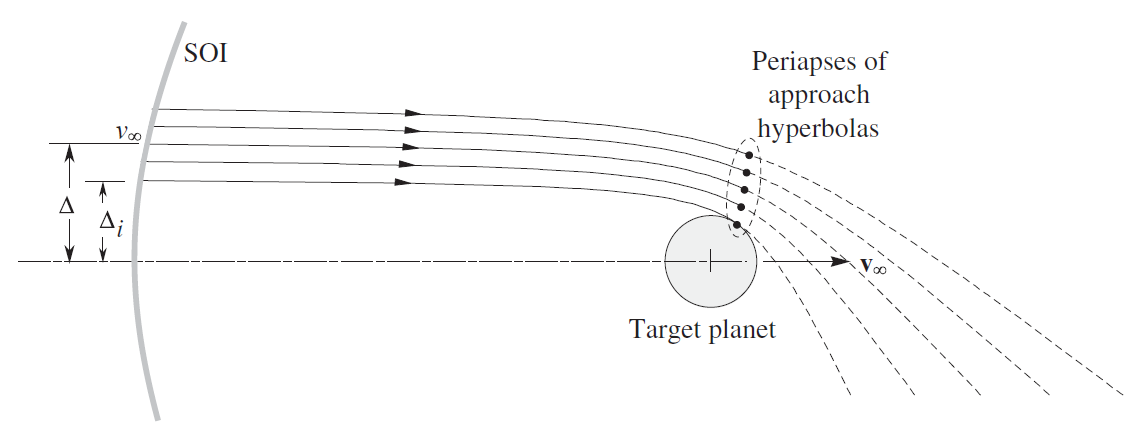
\includegraphics[scale=0.3]{figures/Orbiter/joihyp.png}
\caption{Incoming hyperbolas for varying aiming radius (Howard D. Curtis, Orbital Mechanics for Engineering Students).\cite{orbitals}}
\label{fig:joihyp}
\end{figure}

To get into orbit, the spacecraft needs to fire its engine in the anti-velocity (retrograde) direction and remove the excess delta-V at the hyperbolic periapsis. The amount of delta-V reduction is depending on the type of capture orbit we want to achieve. In our case, the most fuel efficient option will be a highly eccentric orbit (e=0.9) around Jupiter with an orbital period of 165 days. The speed at the periapsis of hyperbolic trajectory is given by the formula:
\begin{equation}
V_{hyp,p}=\sqrt{V_{\infty}^{2}+\frac{2\mu}{r_p}}
\end{equation}
Where $\mu=GM_J$ is the gravity parameter for the Jupiter two body problem. The required speed for an elliptical Jupiter capture orbit is given by the orbital dynamics equations by the formula:
\begin{equation}
V_{capture}=\sqrt{\frac{\mu\left(1+e\right)}{r_p}}
\end{equation}
The difference of the above velocities will give us the required delta-V for Jupiter orbit capture. Note that in these calculations, the incoming asymptote of the Hohmann transfer orbit in the Jupiter reference system is parallel to Jupiter’s orbital track and so the vector subtraction of Jupiter’s orbital and spacecraft asymptotic velocities equals with the absolute values of the velocities subtraction.  Doing the delta-V calculation for the hyperbolic excess velocity given by Petropoulos et al. for the VEMEGA orbit
(\cite{petropoulos2000a}) ($V_\infty=5.58km/s$) we get:
\begin{equation}
\Delta V_{capture}=\sqrt{V_{\infty}^{2}+\frac{2\mu}{r_p}}-\sqrt{\frac{\mu\left(1+e\right)}{r_p}} = \mathbf{1.321 [km/s]}
\end{equation}
\section{Fuel mass calculation}
To calculate the fuel consumption for the required delta-V burn, we use the general rocket thrust equation:
\begin{equation}
F = \dot{m}v_e+(p_e-p_o)A_e
\end{equation}
Where the following engine parameters are required:
\begin{equation}
\begin{split}
\dot{m}&:\text{fuel mass rate}\\
v_e&:\text{equivalent velocity-exit velocity}\\
p_e&:\text{exit pressure}\\
p_o&:\text{free stream pressure}\\
A_e&:exit/nozzle \text{ area ratio}\\
\end{split}
\end{equation}

\begin{figure}[htb!]
\centering
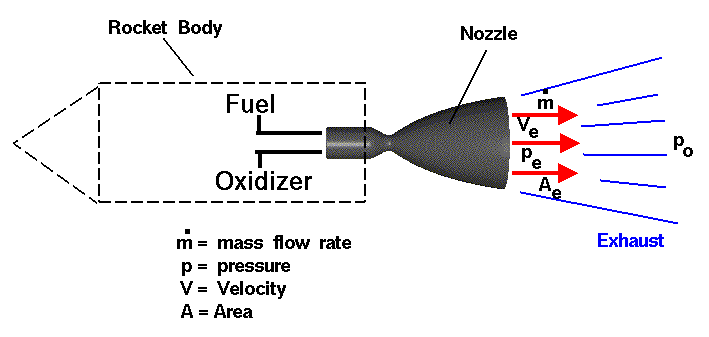
\includegraphics[scale=0.4]{figures/Orbiter/rockth.png}
\caption{Thrust equation schematic diagram (Source:NASA, GRC).\cite{rocketeq}}
\label{fig:rocketim}
\end{figure}

Dividing the thrust equation with the mass rate, we define the equivalent velocity:
\begin{equation}
v_{eq}=\frac{F}{\dot{m}}=v_e+\frac{(p_e-p_o) A_e}{\dot{m}}
\end{equation}
Then, we define the specific impulse parameter, which describes the ratio of thrust produced to the weight of propellant, in seconds using the updated thrust equation:
\begin{equation}
I_{sp}=\frac{v_eq}{g_o} =\frac{F}{\dot{m}g_o}
\end{equation}
Thus, substituting to the thrust equation, we get the thrust written as:
\begin{equation}
F=I_{sp}\dot{m}g_o
\end{equation}
We then employ Newton’s second law of motion:
\begin{equation}
F=m\frac{du}{dt}
\end{equation}
\begin{equation}
\int_{u_o}^{u}du=-\int_{m_o}^{m}\frac{I_{sp}g_o}{m}dm
\end{equation}
So, the total velocity change can be expressed as:
\begin{equation}
\Delta v=-I_{sp}g_o ln(\frac{m}{m_o})
\end{equation}
The final mass of the spacecraft after the required delta-V change will then be:
\begin{equation}
m_{final}=m_{o}e^{-\frac{\Delta v}{v_{eq}}}
\end{equation}
\section{Spacecraft propulsion}
In order to get a realistic fuel required calculation for the JOI burn, we are using an analog of the propulsion system used in the Cassini spacecraft. The total wet mass of the Cassini-Huygens mission was 5712Kg \cite{cassini} and used two engines, one for redundancy.
Cassini's engine characteristics and the Europa Life Finder Mission are shown in the following board:

% Table generated by Excel2LaTeX from sheet 'Ark1'
\begin{table}[htb!]
  \centering
    \begin{tabular}{|c|c|c|}
    \hline
          & \textbf{Cassini} & \textbf{Europa Lander Mission} \bigstrut\\
    \hline
    Engine Thrust (N) & 440   & \textbf{500} \bigstrut\\
    \hline
    Engine Isp (s) & 308   & \textbf{300} \bigstrut\\
    \hline
    Spacecraft wet mass (Kg) & 5574  & \textbf{7300} \bigstrut\\
    \hline
    \end{tabular}%
    \caption{Cassini propulsion comparison.\cite{cassini}}
  \label{tab:propulsion}%
\end{table}%

Using the engine thrust equations, the calculated fuel mass for the JOI burn has the requirements specified in table (\ref{tab:joi_burn_req}).

\begin{table}[htb!]
  \centering
    \begin{tabular}{|c|c|}
    \hline
    \textbf{Engine Thrust Efficiency} & 100\% \bigstrut\\
    \hline
    \textbf{DeltaV Magnitude (Km/s)} & 1321\bigstrut\\
    \hline
    \textbf{Burn duration (min)} & 262.7\bigstrut\\
    \hline
    \textbf{Fuel used (Kg)} & \textbf{2642}\bigstrut\\
    \hline
    \end{tabular}%
    \caption{JOI burn requirements}
  \label{tab:joi_burn_req}%
\end{table}%
\newpage
\section{Possibility of initial Ganymede pump-down flyby}
In order to further reduce the calculated propellant mass required for the JOI burn, there is the possibility of using an initial Ganymede flyby. A flyby at 500Km altitude from Ganymede will save about 400 Km/s of delta-V \cite{clipper} which translates to 928Kg of fuel saved for our mission. As the fuel saving is significant, the Europa Life Finder Mission will use the initial Ganymede flyby. The time coordination of the Ganymede flyby will be further redefined from the pre-arrival Jupiter moons observation campaign and the TCM burns several months before arrival to Jupiter.

\begin{table}[htb!]
  \centering
    \begin{tabular}{|c|c|c|}
    \hline
    \textbf{} & No initial Ganymede flyby & Initial Ganymede flyby \bigstrut\\
    \hline
    \textbf{Engine Thrust Efficiency} & 100\% & 100\% \bigstrut\\
    \hline
    \textbf{DeltaV Magnitude (Km/s)} & 1321  & 921 \bigstrut\\
    \hline
    \textbf{Burn duration (min)} & 262.7 & 197.6 \bigstrut\\
    \hline
    \textbf{Fuel used (Kg)} & \textbf{2642} & \textbf{1963} \bigstrut\\
    \hline
    \end{tabular}%
    \caption{JOI burn requirements with and without an initial Ganymyde pump-down flyby.}
  \label{tab:joi_burn}%
\end{table}%

For figures (\ref{fig:joicloseup}), (\ref{fig:joifull}), the STK software was used to simulate and test our calculations for the JOI burn. Initial conditions were given: 1) the spacecraft total wet mass (7300 Kg), 2) the perijove aim radius (865000 Km), 3) burn time (262.7 min). Also the selected propulsion system was used /ref{tab:propulsion}. The The Summary report of the calculation agrees with our estimated parameters, as seen in figure (\ref{fig:stk_report1}) and (\ref{fig:stk_report2})

\begin{figure}[htb!]
\centering
\includegraphics[scale=0.25]{figures/Orbiter/JOIcloseup.png}
\caption{Simulation of the JOI burn sequence (Ifikratis Kamenidis, STK Software).}
\label{fig:joicloseup}
\end{figure}

\begin{figure}[htb!]
\centering
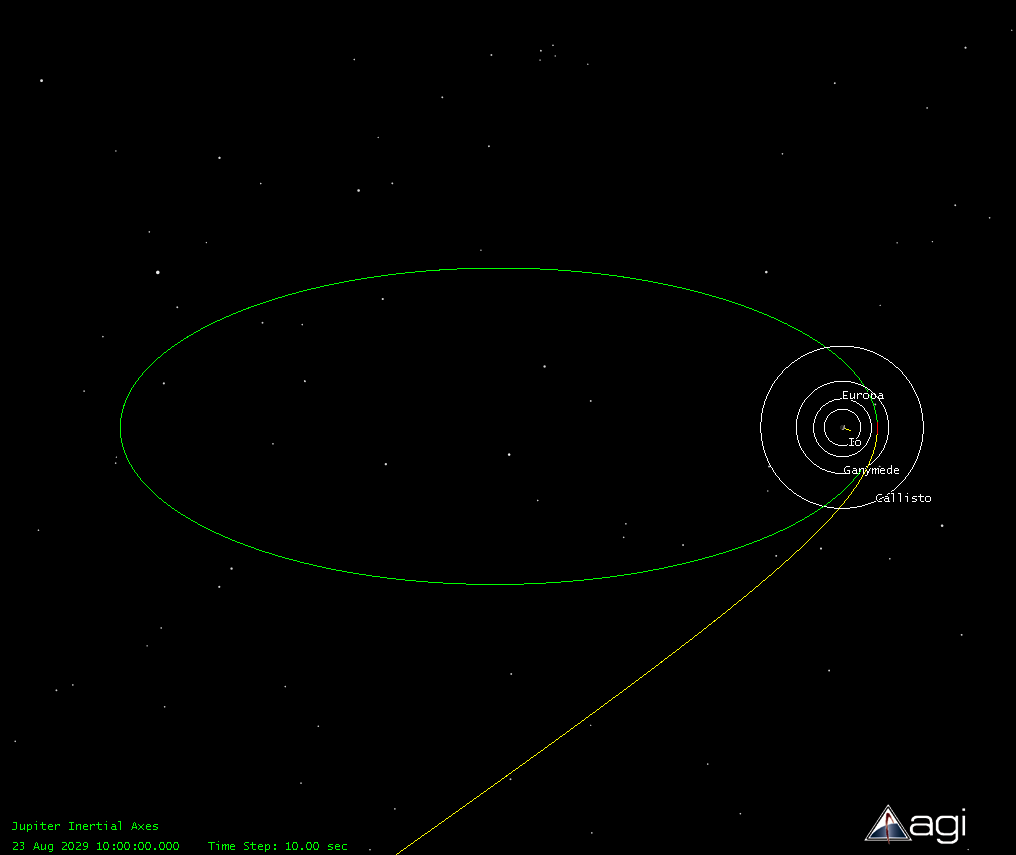
\includegraphics[scale=0.4]{figures/Orbiter/JOIfull.png}
\caption{Simulation of the JOI burn sequence and 165 days capture orbit (Ifikratis Kamenidis, STK Software).}
\label{fig:joifull}
\end{figure}

\begin{figure}[htb!]
\centering
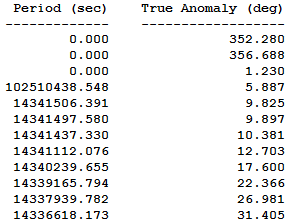
\includegraphics[scale=0.5]{figures/Orbiter/captorb.png}
\caption{STK Orbital period calculation report before and after JOI. The simulation agrees with the 165 days target initial orbit(Ifikratis Kamenidis, STK Software).}
\label{fig:stk_report1}
\end{figure}
\begin{figure}[htb!]
\centering
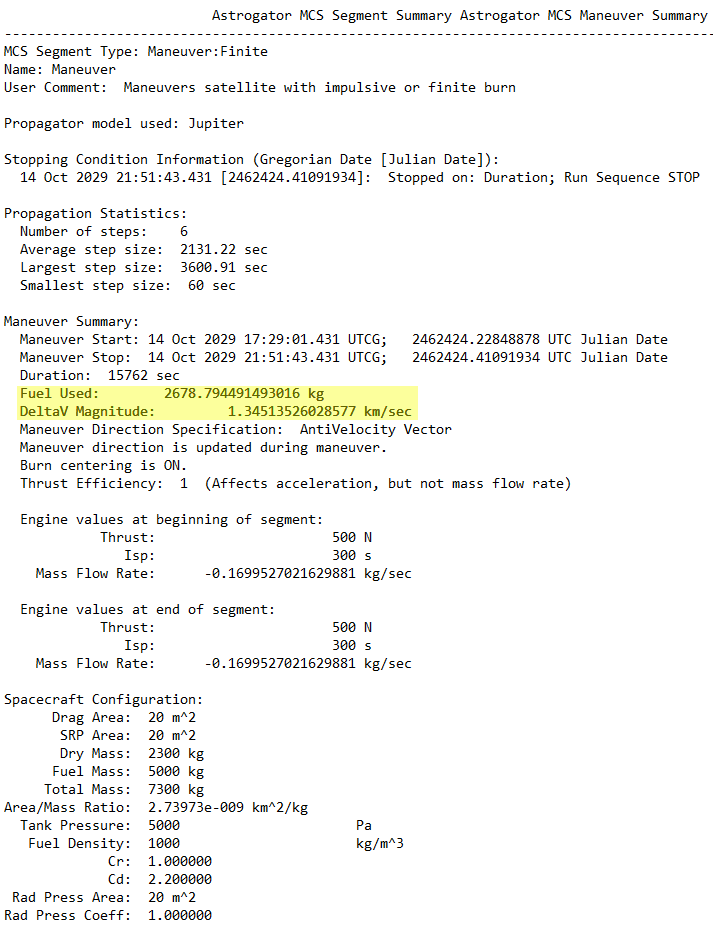
\includegraphics[scale=0.5]{figures/Orbiter/JOIres.png}
\caption{The summary report of JOI burn agrees with our predicted values.(Ifikratis Kamenidis, STK Software).}
\label{fig:stk_report2}
\end{figure}
\section{Jupiter Capture Orbit}
 The selection of the equatorial plane for the Jupiter orbit insertion was done based on the orbiter's mission goals, which is to characterise Europa’s through multiple flybys and deploy a lander into its surface. The only viable way from an orbital mechanics point of view to intercept Europa many times, achieve a good surface coverage before landing and deploy a lander using the least amount of carrying fuel is a by using a low -relative to Europa- inclination orbit around Jupiter. While a polar orbit would better avoid the high radiation lobes of the Jupiter magnetosphere, the above criteria could not be met. An orbit around Europa was ruled out based on the extremely high radiation levels. The JOI burn was designed taking into account the above orbital mission requirements while saving fuel using the opportunity of an initial Ganymede flyby. The capture orbit parameters, and especially the eccentricity of 0.6 was chosen as a realistic trade-off between orbital period and fuel required. A higher eccentricity orbit would require less fuel but would lead to a very high orbital period around Jupiter, prolonging the start of the Europa mission for more than 2 years. On the other hand a lower eccentricity orbit would spare a significant amount of fuel to lower the eccentricity.
\section{Post-Capture orbital design}
Right after the successful completion of the 197min JOI burn, the spacecraft has been captured in the initial 165 days orbit. However, the missions goal's wouldn't be achieved by staying in this long period orbit. The orbital plan is to use the more massive of the Jovian satellites, Ganymede, multiple times to slow the spacecraft down and bring it to a Europa 3:1 resonant orbit around Jupiter. For this scenario to be successful, the spacecraft should use a minimum amount of fuel to fine tune the Ganymede flybys and achieve most of the $\Delta V$ reduction from the close Ganymede encounters. 
\section{Post-Capture orbits progression analysis}
Just by letting the spacecraft orbit Jupiter in a 165 days orbit, will require significant amount of fuel to target a Ganymede flyby, as the relative positions of the spacecraft and Ganymede would be completely random. For that reason, the JOI burn and arrival time are properly targeted during cruise's TCM so that the spacecraft will pass close to Ganymede in the first inbound leg of the capture orbit just before it completes its first 165 orbit. However, the JOI burn and a potential initial Ganymede flyby create unavoidably a post-capture $\Delta V$ error. This  error would be easy to take out in the first apojove pass, targeting the first Ganymede post-orbit pump-down flyby. At this point, the amount of $\Delta V$ required to plan the Ganymede flyby is small enough (analysis follows) to easily achieve a very close Ganymede flyby and so achieve the maximum $\Delta V$ reduction. However, thinking more wisely, such a manoeuvre will not result in the maximum fuel efficiency in the long term. The resulting orbit will then need a significant amount of fuel to plan a next Ganymede (or other moon) flyby, as the orbits will again be chaotic. Spending a huge amount of fuel will unpredictably add mass to the mission while on the other hand, waiting for many orbits for a next opportunity will shift the mission lifetime and risk its successful completion, mainly because of the accumulating radiation of Jupiter's magnetosphere.

It is evident that a more ahead-planning scenario is required. We solve this problem by performing the initial Ganymede flyby in a more reasonable way. Instead of trying to achieve the maximum $\Delta V$ reduction, we plan the first Ganymede flyby in the appropriate aiming radius for a resulting Ganymede resonant orbit. By doing so, we make sure that the next orbit will not be random, but will have an orbital period which will be an integral multiple of Ganymede's orbit around Jupiter (Ganymede resonant orbit). This coherence, assures that the spacecraft can use Ganymede again for a further $\Delta V$ reduction in the next orbit with minimum fuel required. By repeating the same scheme for the 2nd Ganymede flyby, the spacecraft is again on track for a next flyby. Any excess, post flyby $\Delta V$ is managed in the apojove pass, where a small burn is performed to fine-tune the upcoming flyby. The above orbital design will allow the spacecraft to flyby Ganymede every time with the least amount of fuel. After an achieved resonance of 4:1, a flyby with Europa is within reach, and by performing small burns and a pi-transfer Ganymyed flyby, the final Europa resonance orbit will be achieved. 
\newpage
\section{Post-Capture and fuel mass calculations}
In order to test the post-capture orbits scenario viability and perform a detailed analysis of the fuel required for the correction manoeuvres, the STK software (version 10.1.3), a physics-based software geometry engine. For the orbits simulations the Astrogator (v10.0) extension was used. 

Except Jupiter, the four largest Jovian moons gravity models was used in the simulation, to accurately simulate perturbation effects in the orbits evolution. A 7th order Runge-Kutta-Fehlberg integrator with 8th order error control with 1 sec minimum stepsize was used to propagate the spacecraft's motion in Jupiter's gravity field as well as when inside the Sphere of Influence of Ganymede and Europa, when their specific gravity fields were used (\ref{app:sphere_of_infl}). The gravity fields used can be seen in table (\ref{tab:gravf}). Furthermore, a spherical solar radiation pressure (SRP) is used with a dual-cone shadow model.

% Table generated by Excel2LaTeX from sheet 'Sheet1'
\begin{table}[htb!]
  \centering
    \begin{tabular}{|c|c|c|c|}
    \hline
    \multicolumn{4}{|c|}{\textbf{Gravity models}} \bigstrut\\
    \hline
    \textbf{Object} & \textbf{Gravity Model} & \textbf{Degree} & \textbf{Order} \bigstrut\\
    \hline
    \textbf{Jupiter} & JUP230.grv & 6     &  \bigstrut\\
    \hline
    \textbf{Io} & JUP230.grv & 6     &  \bigstrut\\
    \hline
    \textbf{Europa} & Science1998.grv & 4     & 2 \bigstrut\\
    \hline
    \textbf{Ganymede} & Nature1996.grv & 4     & 2 \bigstrut\\
    \hline
    \textbf{Callisto} & JUP230.grv & 6     &  \bigstrut\\
    \hline
    \end{tabular}%
    \caption{Gravity models used in simulation(source: NASA, Horizons, NAIF).\cite{Gravm}}\label{tab:gravf}
\end{table}%

In order to perform the required orbits and manoeuvres calculations by the simulation engine, a series of commands are written in a logical sequence. The software uses a differential corrector to solve a problem of initial conditions, given a set of orbital goals. 
The core of the commands can be synopsised in the following sequence:

\begin{itemize}
  \item Propagate at orbit apojove
  \item Initiate burn - 3 degrees of freedom
  \item Propagate at Ganymede Sphere of Influence radius
  \item Target flyby B-plane - specific BdotR, BdotT goals are set
  \item Propagate at apoJove
\end{itemize}

At the end of each iteration, the resulting orbital period is checked. $B\cdot R$ and $B\cdot T$ targets are altered until the desired orbital period is achieved. Then, the same iteration sequence is run for calculating the upcoming Ganymede flyby. The achieved resonances of orbit two, three and four (orbit one equals to capture orbit) are 9:1, 6:1 and 3:1 respectively. 
Table (\ref{tab:boardm}) shows an overview of the apoJove burns and flyby $\Delta V$ parameters. Assumed 5426Kg wet mass after JOI burn in the Ganymede initial pump-down scenario. The new wet mass after a burn is always taken into account in the calculations. Engine ISP=300s and Engine thrust=500N. OX-BX indicate the apoJove burns, while with GX and EX are noted the in sequence Ganymede and Europa flybys.

% Here, I want the table to appear after the text above, but its not
%one second
% Table generated by Excel2LaTeX from sheet 'Sheet1'
\begin{table}[htb!]
  \centering
    \begin{tabular}{|r|r|r|r|r|}
    \hline
          & \boldmath{}\textbf{$\Delta V (m/s)$}\unboldmath{} & \textbf{Burn time(s)} & \textbf{Fuel used (Kg)} & \textbf{Range (Km)} \bigstrut\\
    \hline
    \multicolumn{1}{|c|}{\textbf{O1-B1}} & \multicolumn{1}{c|}{4.409015} & \multicolumn{1}{c|}{29.926} & \multicolumn{1}{c|}{8.114} & \multicolumn{1}{c|}{} \bigstrut\\
    \hline
    \multicolumn{1}{|c|}{\textbf{G1}} & \multicolumn{1}{c|}{794.84} & \multicolumn{1}{c|}{} & \multicolumn{1}{c|}{} & \multicolumn{1}{c|}{2268} \bigstrut\\
    \hline
    \multicolumn{1}{|c|}{\textbf{O2-B2}} & \multicolumn{1}{c|}{0.724688} & \multicolumn{1}{c|}{4.919} & \multicolumn{1}{c|}{1.334} & \multicolumn{1}{c|}{} \bigstrut\\
    \hline
    \multicolumn{1}{|c|}{\textbf{G2}} & \multicolumn{1}{c|}{494.89} & \multicolumn{1}{c|}{} & \multicolumn{1}{c|}{} & \multicolumn{1}{c|}{3189} \bigstrut\\
    \hline
    \multicolumn{1}{|c|}{\textbf{O3-B3}} & \multicolumn{1}{c|}{4.197475} & \multicolumn{1}{c|}{28.49} & \multicolumn{1}{c|}{7.725} & \multicolumn{1}{c|}{} \bigstrut\\
    \hline
    \multicolumn{1}{|c|}{\textbf{G3}} & \multicolumn{1}{c|}{1223.24} & \multicolumn{1}{c|}{} & \multicolumn{1}{c|}{} & \multicolumn{1}{c|}{489} \bigstrut\\
    \hline
    \multicolumn{1}{|c|}{\textbf{O4-B4}} & \multicolumn{1}{c|}{1.180696} & \multicolumn{1}{c|}{8.014} & \multicolumn{1}{c|}{2.17} & \multicolumn{1}{c|}{} \bigstrut\\
    \hline
    \multicolumn{1}{|c|}{\textbf{G4}} & \multicolumn{1}{c|}{1080.2} & \multicolumn{1}{c|}{} & \multicolumn{1}{c|}{} & \multicolumn{1}{c|}{497} \bigstrut\\
    \hline
    \multicolumn{1}{|c|}{\textbf{O5-B5}} & \multicolumn{1}{c|}{103.7305} & \multicolumn{1}{c|}{1146} & \multicolumn{1}{c|}{187.376} & \multicolumn{1}{c|}{} \bigstrut\\
    \hline
    \multicolumn{1}{|c|}{\textbf{E1}} & \multicolumn{1}{c|}{804.61} & \multicolumn{1}{c|}{} & \multicolumn{1}{c|}{} & \multicolumn{1}{c|}{627} \bigstrut\\
    \hline
    \multicolumn{1}{|c|}{\textbf{O6-B6}} & \multicolumn{1}{c|}{149.8431} & \multicolumn{1}{c|}{1644} & \multicolumn{1}{c|}{256.233} & \multicolumn{1}{c|}{} \bigstrut\\
    \hline
    \multicolumn{1}{|c|}{\textbf{E2}} & \multicolumn{1}{c|}{45.98} &       & \multicolumn{1}{c|}{} & \multicolumn{1}{c|}{3771} \bigstrut\\
    \hline
    \multicolumn{1}{|c|}{\textbf{Total }} & \multicolumn{1}{c|}{4707.8} &       & \multicolumn{1}{c|}{462.952} & \multicolumn{1}{c|}{} \bigstrut\\
    \hline
    \end{tabular}%
    \caption{Resulting burn parameters for post-Jupiter capture orbits progression.}
  \label{tab:boardm}%
\end{table}%

\begin{figure}[htb!]
\centering
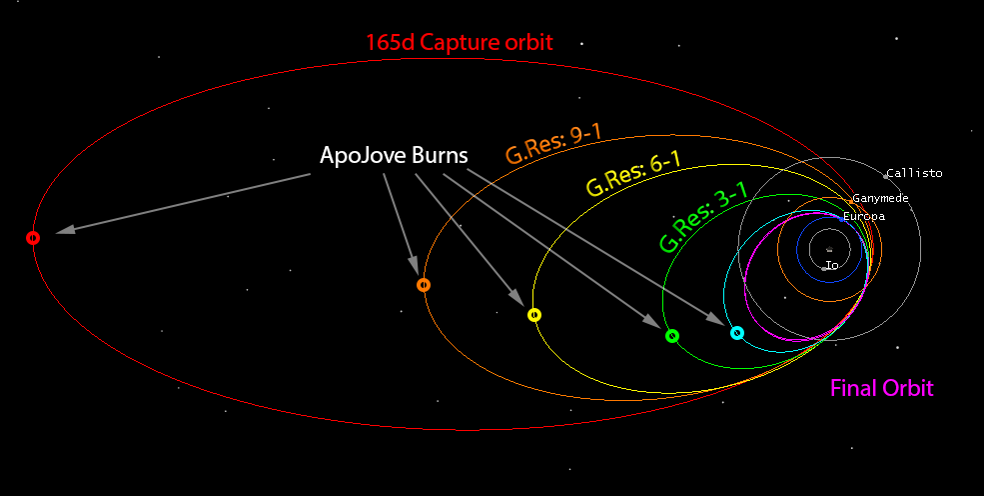
\includegraphics[width=\textwidth]{figures/Orbiter/orbits.png}
\caption{Orbits evolution from JOI to Europa target 3:1 resonance orbit. (Ifikratis Kamenidis, STK Software).}\label{fig:orbits_resonance}
\end{figure}
\begin{description}[align=left]
\item [Post-capture orbital design]\hfill \\
An animation of the post-capture orbital design can be seen at:

\url{https://www.youtube.com/watch?v=sUmYL08Vr14}
\item [Ganymede Flyby]\hfill \\
Also, an animation of a 500Km Ganymede flyby can be seen at:

\url{https://www.youtube.com/watch?v=64JcLukSnnY}.
\end{description}
\section{Arriving at target orbit}
After the completion of the third Ganymede flyby, the forth Ganymede flyby is performed with a dual purpose. First to further reduce the apojove distance of the orbit and at the same time place the spacecraft in an orbit to intercept Europa for the first time. Meanwhile, every Ganymede flyby is lowering the perijove of the orbit, while the last Ganymede flyby brings the perijove at approximately 9.3 $R_J$ in Europa's vicinity. The first Europa flyby itself is designed to provide the necessary $\Delta V$ reduction to place the spacecraft in the target 3:1 resonant Europa orbit. For every spacecraft orbit around Jupiter, Europa make exactly three orbits. This synchronisation is key in achieving a continuous flybys in order to provide the orbiter the ability to do pre-landing reconnaissance and find the best landing site location for the lander module. After landing, the same orbit will be used to provide the communication link between the penetrator -lander and the Earth. The orbital parameters of the target orbit can be seen in table (\ref{tab:eurorb}).

% Table generated by Excel2LaTeX from sheet 'Sheet1'
\begin{table}[htb!]
  \centering
    \begin{tabular}{|c|c|}
    \hline
    Semi-major axis (Km) & \textbf{1,392,748} \bigstrut\\
    \hline
    PeriJove (Km) & \textbf{662,300} \bigstrut\\
    \hline
    ApoJove (Km) & \textbf{2,525,000} \bigstrut\\
    \hline
    Eccentricity & \textbf{0.5244} \bigstrut\\
    \hline
    Inclination ($^\circ)$ & \textbf{3.816} \bigstrut\\
    \hline
    Period (days) & \textbf{10.6} \bigstrut\\
    \hline
    TID under 2cm of Al (krad/month) & \textbf{5.2} \bigstrut\\
    \hline
    Europa flyby relative $\Delta V$(Km/s) & \textbf{3.3} \bigstrut\\
    \hline
    \end{tabular}%
    \caption{Europa 3:1 resonant orbit parameters.}
  \label{tab:eurorb}%
\end{table}%
\begin{figure}[htb!]
\centering
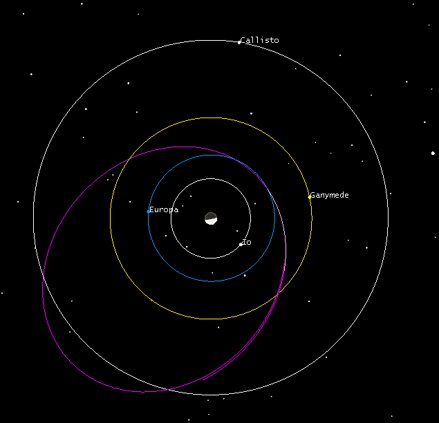
\includegraphics[scale=1]{figures/Orbiter/europares.png}
\caption{Europa 3:1 resonant orbit (Ifikratis Kamenidis, STK Software).}
\end{figure}
\section{Perturbations and orbit sustainability}
Europa's mass is significant enough to alter the spacecraft's trajectory every time it flies by the moon. The gravity assist was useful for the initial pump-down and orbital decay of the capture orbit as explained in the previous chapter. However, in the case of the target orbit, unavoidably a $\Delta V$ change will occur after every flyby. As a result, the apojove radius will now change, hence the orbital period and the 3:1 resonance synchronization. An apojove burn will be necessary in every orbit to keep the spacecraft in the resonant trajectory. In that case the amount of fuel required will be very large. Moreover, besides sustaining the orbit the goal of the orbiter's flyby is to map the surface prior to landing, and so a method of placing the groundtrack of a hyperbolic orbit over desired latitudes and longitudes has been developed by NASA \cite{cotseq}. 

The flyby sequence called "Crank-over-the-top Sequence" (COT) and was used bt the Cassini mission for the Titan flybys. The technique is implemented by cranking the inclination of the orbit starting from a n equatorial point and arriving at a maximum inclination ($i_{max}$). The incoming and outcoming v-infinity velocities have the same pump angle (\ref{fig:pump_a}).
and the total $\Delta V$ is perpendicular to the moon velocity (\ref{fig:cotgeo}). 
%\todo[inline]{graphs 5.19 & 5.20 do not appear here}

\begin{figure}[htb!]
    \centering
    \captionsetup[subfigure]{width=0.45\textwidth}
    \subfloat[Pump angle \cite{cotseq}.]{
        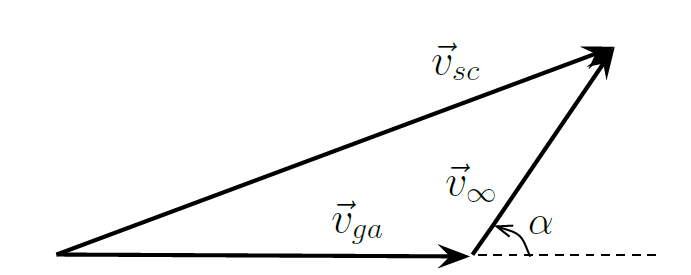
\includegraphics[width=.48\textwidth]{figures/Orbiter/pumpa.png}
        \label{fig:pump_a}
    }
    \subfloat[COT sequence flyby geometry \cite{cotseq}.]{
        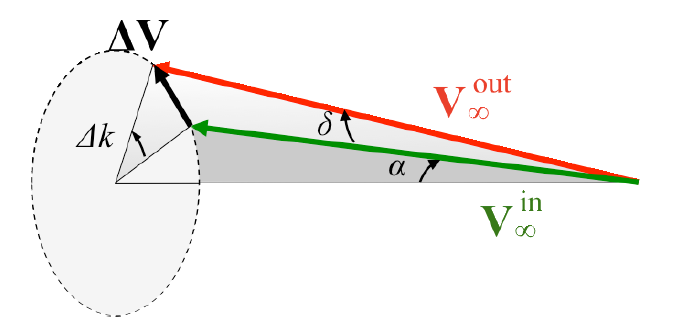
\includegraphics[width=.48\textwidth]{figures/Orbiter/flbeom.png}
        \label{fig:cotgeo}
    }
    \caption{Flyby geometry}
\end{figure}

The COT sequence will begin will outbound flybys and cover the anti-jovian facing hemisphere of Europa which is tidally locked. The groundtracks as calculated by Brent Buffigton et al. \cite{cotseq} can be seen at figure \ref{fig:ground_tr} for a 3:1 resonant Europa COT sequence.

\begin{figure}[htb!]
\centering
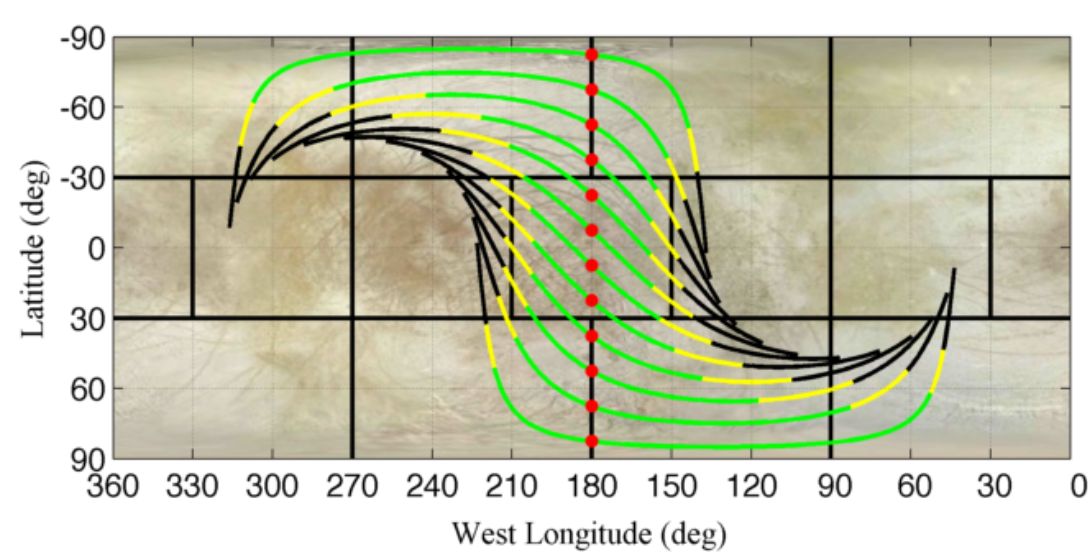
\includegraphics[scale=0.3]{figures/Orbiter/groundtr.png}
\caption{Grountracks of a COT sequence in a 3:1 resonant Europa jovian orbit \cite{cotseq}.}
\label{fig:ground_tr}
\end{figure}

Furthermore, illumination of the moon is a crucial part of the reconnaissance as long as the landing phase. As Europa rotates around Jupiter the antijovian hemisphere will experience a 3.5 days day-night period. As shown before, the resonant orbit's perijove is also the flyby point. That means that changing the orbit's argument of periapsis ($\omega$) the line of nodes can be rotated. While at the same time keeping the resonance of the orbit, the orbiter can experience different illumination conditions on the antijovian Europa hemisphere. This shift can be achieved by using the COT sequence by cranking up the inclination and pumping down the orbit period in order to use a Europa to Ganymede pi-transfer \cite{cotseq}. As the lander requirements is find a landing spot in the antijovian hemisphere, the lighting conditions change will not require an 180 degree shift for a full moon coverage. Instead a total of 90 degree of Europa illumination rotation would be sufficient.  
\section{Flyby geometrical configuration}
As the orbiter flybys Europa, the physical orientation of the spacecraft should be maintained in order to fulfil mission goals. This is especially important in the pre-landing phase of the mission, when the ERIS (Europa Reconnaissance Imaging System) will be used to cover the surface and find candidate landing sites. 

Depending on the flyby coverate goal, a flyby can either target the leading edge hemisphere of Europa or the trailing edge. Both configurations are designed to map the antijovian facing hemisphere of Europa, as this is where a landing site is more favorable (less radiation and bigger communication windows). The leading edge hemisphere also shows a lower radiation as the fast rotation of Jupiter and so its magnetic field will hit mainly the trailing hemisphere on the 3.5 days orbit around Jupiter. Figures \ref{flyby1} and \ref{flyby2} show the two different flyby geometries. In the first case (\ref{flyby1}) the orbiter will have more time to image Europa on the outbound leg of the flyby (red) while in the second case (\ref{flyby2}) the orbiter will have more time to image Europa in the inbound leg of the flyby. Thus, the selection should be made according to flyby reconnaissance targets but also depending on the illumination of the moon the specific flyby time. Terminator areas are preferred for showing texture and shadows in interesting areas.
%\todo[inline]{pictures 5.22 and 5.23 do not appear here}
\begin{figure}[htb!]
\centering
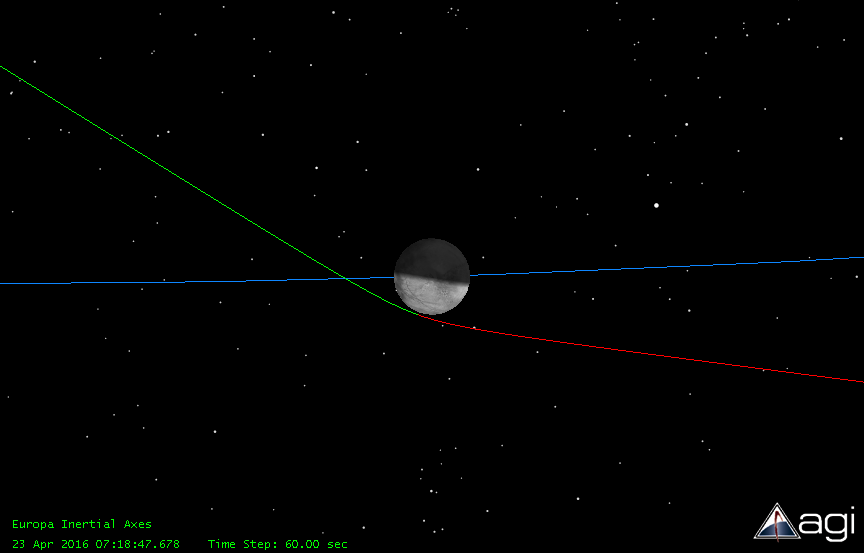
\includegraphics[width=0.9\textwidth]{figures/Orbiter/flyby1.png}
\caption{Flyby geometry targeting the leading edge antijovian hemisphere (Ifikratis Kamenidis, STK software).}
\label{flyby1}
\end{figure}

\begin{figure}[htb!]
\centering
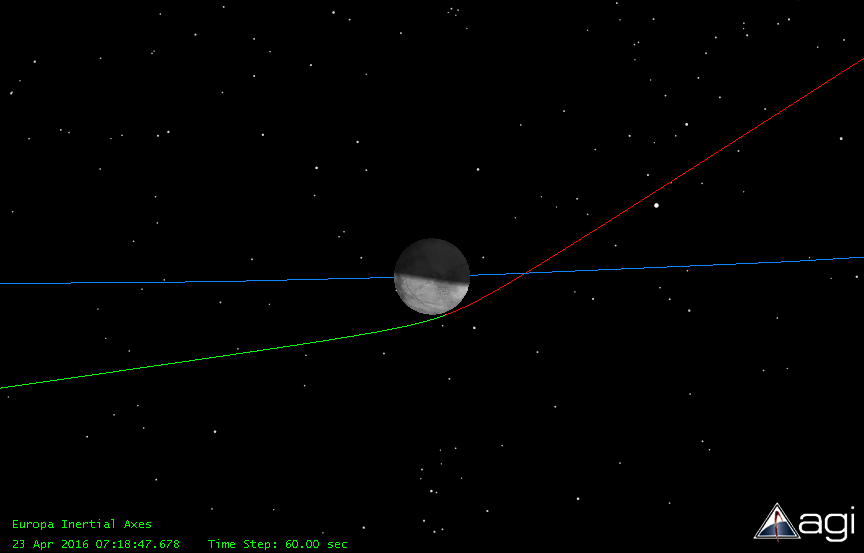
\includegraphics[width=0.9\textwidth]{figures/Orbiter/flyby2.png}
\caption{Flyby geometry targeting the trailing edge antijovian hemisphere (Ifikratis Kamenidis, STK software).}
\label{flyby2}
\end{figure}
As the orbiter flybys Europa, the orientation of the cameras and so of the spacecraft is paramount for achieving the precise targeting. We are interested in maximizing coverage by the least amount of flybys to prolong mission life (less TID possible) as the mission goal is to land on the surface and reach the subsurface ocean by a penetrator. 
Two different imaging geometry configurations are considered. 

One solution is to implement a steady top down imaging of both narrow angle (high resolution) and wide angle (low resolution) cameras. The achieved coverage for a trailing edge inbound flyby can be seen in \ref{steadycov}. The pointing accuracy for such a configuration requires that the spacecraft will rotate in its yaw axis, based on the angular velocity of the spacecraft in respect to the Europa reference system. 

Another option is to initiate a double rotation of the spacecraft (and so the cameras). This maneuver does not pose any danger to the mission as; 1) the orbiter is powered by RTG so pointing to the sun is not necessary 2) high-gain antenna link to the Earth can be skipped for the duration of the flyby which is less than 30 minutes 3) there is no need to communicate with the lander, as the reconnaissance phase happens before lander separation. The maneuver requires the spacecraft to initiate two rotations in roll and yaw and a small pitch maneuver; First a small yaw rotation (non linear) which tracks Europa's center of gravity takes place (less than 0.1rpm - depending on flyby target radius (see figure \ref{flybyangle})) and second a roll revolution of 1 rpm. Third, placing the camera's pointing axis in an offset angle will result in a rotational effect imaging pattern. The ground area coverage for this configuration can be seen in figure \ref{rot_cover}. The angular momentum requirements can be seen in figure \ref{flybyangle} while the relative speed for a flyby aiming radius of 100Km flyby can bee seen in figure \ref{flybyspeed}.

\begin{figure}[htb!]
\centering
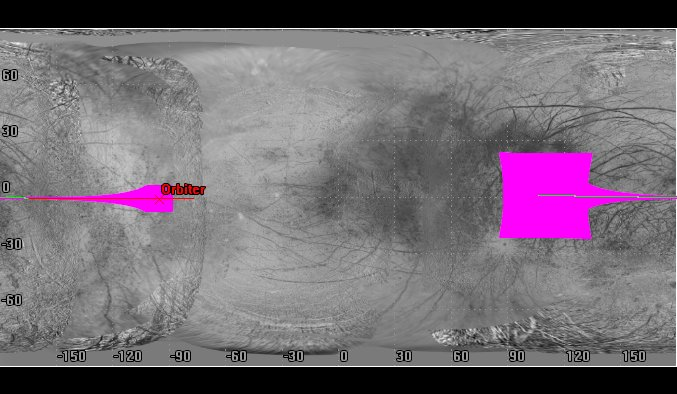
\includegraphics[width=0.9\textwidth]{figures/Orbiter/steady_cover.png}
\caption{Ground area coverage for one flyby using a steady top-down pointing. FOV:5 degrees. Inclination is zero degrees relative to Europa (Ifikratis Kamenidis, STK software).}
\label{steadycov}
\end{figure}
\begin{figure}[htb!]
\centering
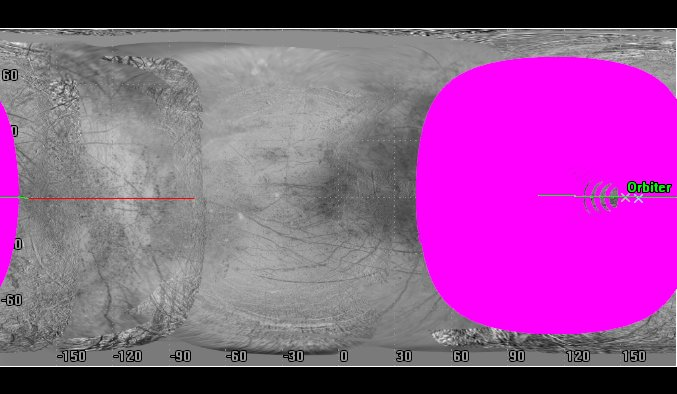
\includegraphics[width=0.9\textwidth]{figures/Orbiter/rot_cover.png}
\caption{Ground area coverage for one flyby using rotating pointing. FOV:5 degrees, rotation rate is 1rpm. Inclination is zero degrees relative to Europa(Ifikratis Kamenidis, STK software).}
\label{rot_cover}
\end{figure}

3D flyby animations of the two imaging geometries can be seen at:
\begin{description}[align=left]
\item [Steady top-down pointing:]\hfill \\
\url{https://www.youtube.com/watch?v=LjMV9DhwkUo}.
\item [Rotating pointing:]\hfill \\
\url{https://www.youtube.com/watch?v=hLvxofgHwf8}.
\end{description}


\begin{figure}[htb!]
\centering
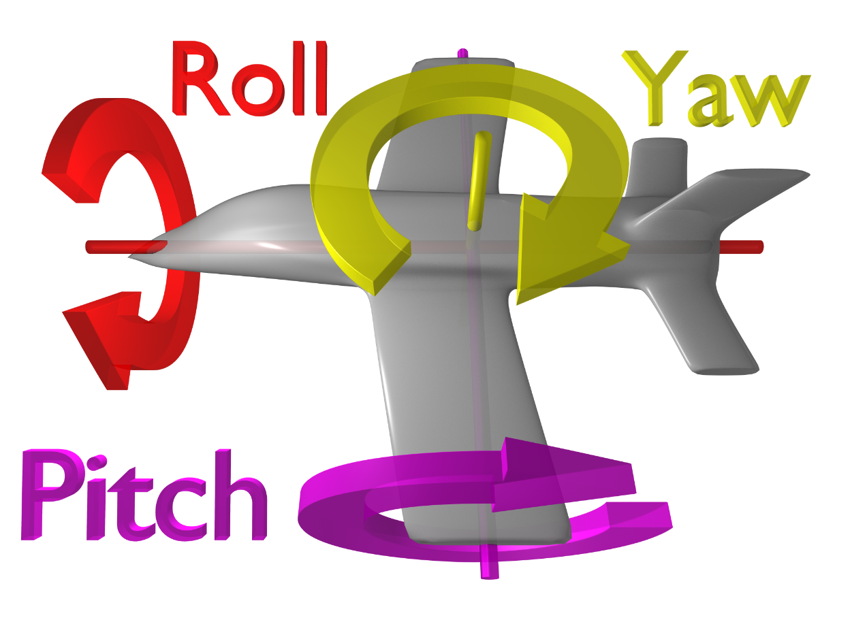
\includegraphics[scale=0.5]{figures/Orbiter/axis_o.png}
\caption[Spacecraft pitch, yaw and roll axis]{Spacecraft pitch, yaw and roll axis \footnote{wikipedia, Author:ZeroOne}.}
\label{axis_o}
\end{figure}

\begin{figure}[htb!]
\centering
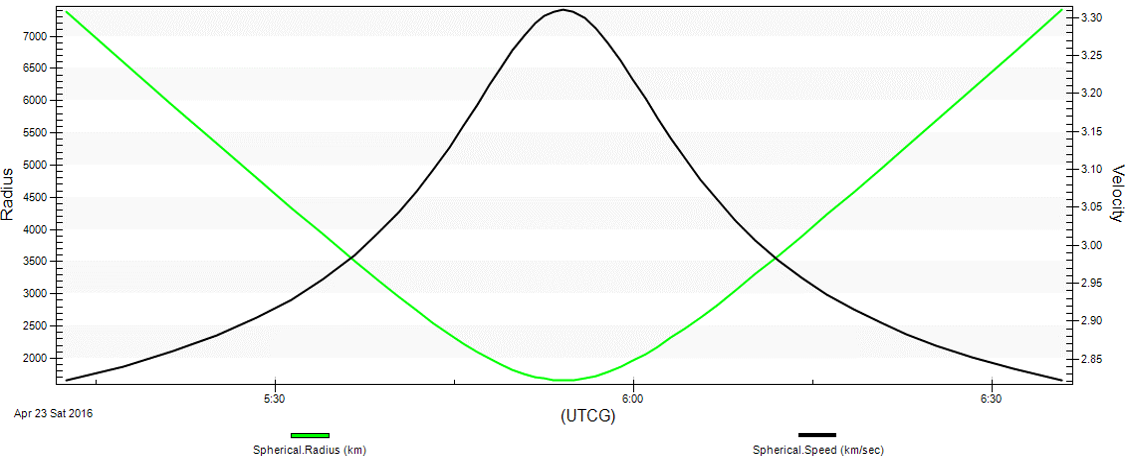
\includegraphics[width=\textwidth]{figures/Orbiter/flybyspeed.png}
\caption{Speed and Radius plot for a 100Km altitude flyby (Ifikratis Kamenidis, STK software).}
\label{flybyspeed}
\end{figure}

\begin{figure}[htb!]
\centering
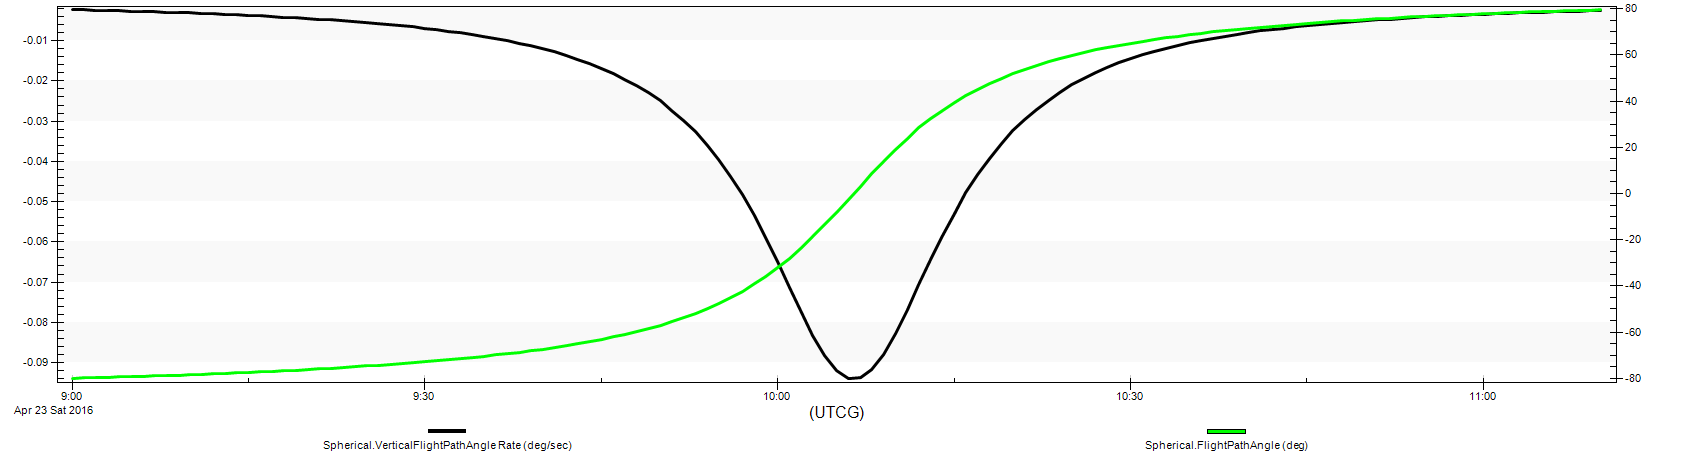
\includegraphics[width=\textwidth]{figures/Orbiter/anglerate2.png}
\caption{Angle change and angle rate for a 100Km altitude flyby (Ifikratis Kamenidis, STK software).}
\label{flybyangle}
\end{figure}
\section{Implementation (Orbital Mechanics)}
\chapter{Analysis of the Surface Environment}%
%\section{Analysis of Europa Moon surface and Environment}
\section{The Radiation Environment}\label{sec:radiation_environment}
Jupiter’s magnetic field, shaped as a toroidal, affects the radiation environment around the planet by interacting with the solar wind trapping energetic particles, creating radiation belts similar to van Allen belts on Earth but with much higher intensity. This magnetosphere of charged particles extends radially from 50 to 100 RJ. For purpose of practicality this area is subdivided into three main regions, the outer magnetosphere ($>$40 RJ), middle (10-40 RJ) and the inner magnetosphere ($<$10 RJ). For our purpose, we are focusing on the middle region, an area where Europa lays along with the rest of the four Galilean moons, Io, Ganymede and Calisto. Highly energetic charged particles are trapped within that region, mainly electrons and protons but also ions, ranging from a few keV up to tens of MeV. Here we can also locate the Io plasma torus, created by the interaction of the rotating magnetic field of Jupiter with the spewed volcanic gasses of Io, drifting and ionizing them into plasma.

Axial tilt of the magnetic dipole of Jupiter and consequently of the spin plane, causes Europa to cruise in and out of the plane by 10$^circ$ north and south of the magnetic latitude affecting the radiation environment of the moon. 

Through a process known as sputtering, bombardment of Europa’s surface with highly ionizing particles causes the ejection of surface molecules where some of them manage to escape gravitational pull of the moon and get accelerated by the co-rotating magnetosphere creating an additional contribution to the particle distribution. 

Data collected by Galileo, Voyager and Pioneer spacecraft missions show high intensities of energetic particles fluxes around Europa’s orbit area varying in time to a limited extent. Electrons intensity (fig. \ref{electrons energy}) show a wide spectra of energies dominating on that region but with a large variation on lower energies due to the high uncertainty rates of the detectors during these missions and especially from Galileo.
\begin{figure}[htb]
\centering
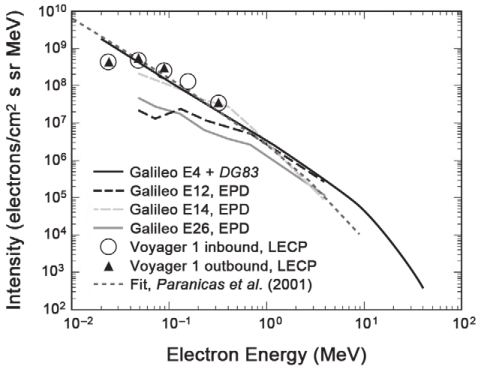
\includegraphics[width=0.5\textwidth]{figures/Orbiter/electrons_energy_spectrum}
\caption{Energy spectrum of electrons near Europa’s orbit from various sources, \cite{paranicas2009europa}.}
\label{electrons energy}
\end{figure}
Several Galileo close encounters to Europa’s orbit, reveal the energy distribution of proton, oxygen and sulfur ions and show high intensities at high energies while on low energies a greater variation between the ions is observed (fig. \ref{fig:ions_energy}).
\begin{figure}[htb]
    \centering
    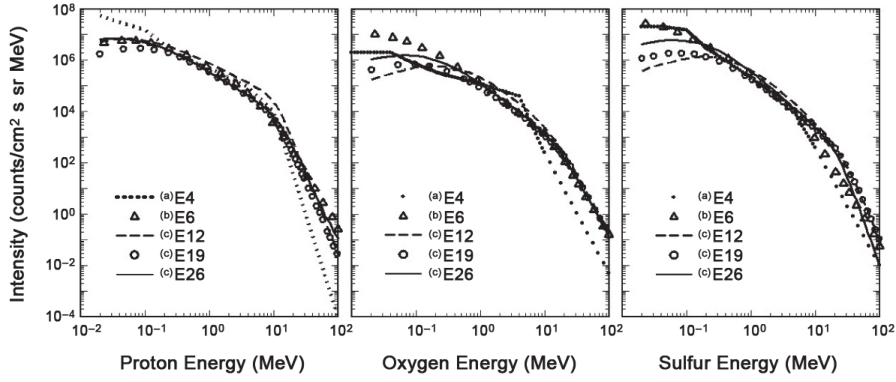
\includegraphics[width=0.80\textwidth]{figures/Orbiter/ions_energy}
    \caption{Ion energy spectra data acquired from Galileo mission on various encounters of Europa at distances of 692 km (E4), 586 km (E6), 201 km (E12), 1439 km (E19), and 351 km (E26) \cite{paranicas2009europa}}
    \label{fig:ions_energy}
\end{figure}
\section{Current Studies of the Surface}\label{sec:surface_studies}
Delivering a lander vehicle on Europa, requires a thorough knowledge of the surface composition and characteristics. On a large scale the surface looks smooth and without great variations but on a higher spatial resolution we can notice the complexity of the terrain. Smooth plains, lenticulae and chaos regions dominate the morphology and topography of the moon’s surface. Many models have suggested that formation of these terrain features involves hydrothermal activity within the ice shell causing fractures and ridges (fig\ref{fig:europa_surface}). 
\begin{figure}[htb]
    \centering
    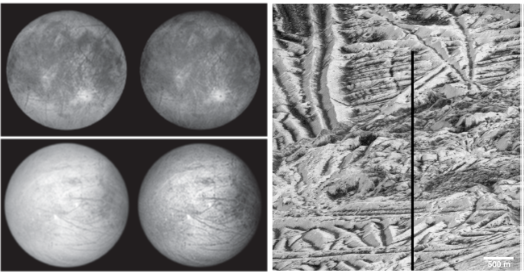
\includegraphics[scale=0.6]{figures/Orbiter/europa_surface.png}
    \caption{Left: Europa’s trailing (top) and leading (bottom) hemispheres as imaged from Galileo on the left and enhanced on the right to illustrate the geological complexity of the surface. Right: A close up look of the surface \cite{carlson2009europa}}
    \label{fig:europa_surface}
\end{figure}
Studies of the surface composition, suggest that Europa was formed by endogenic and exogenic sources of materials. Endogenic sources include either thermochemical reactions that have created hydrated silicates, iron oxides and carbon-nitrogen compounds or unaltered silicates, nickel-iron compounds, organic matter and water, depending on the initial conditions of the protojovian nebula. As for exogenic material, three main sources have been identified. Io’s ejected material reaching Europa by its thermal plasma torus, material outside of the Jovian system delivered by comets and asteroids, and material from the outer Jovian satellites ejected from their surfaces.
%\todo[inline]{Other missions - Galileo et al.}
\section{Lenticulae}\label{sec:lenticulae}
On the surface of Europa a number of circular and elliptical formations are observed, named as lenticulae (fig. \ref{fig:lenticulae}). Many of these are domed hills, cavities and others seems to be dark and flat blemishes. Some appear to have a rough surface with a chaotic structure. The peaks of these domes, show similarities with the composition of the nearby surface, indicating that they have been probably created when the crust forced from below due to some geological events, similar to the magma chambers on Earth. Origin of the flat dark blemishes seems to be melted ice that has been released from cracks of the surface.
\begin{figure}[htb]
    \centering
    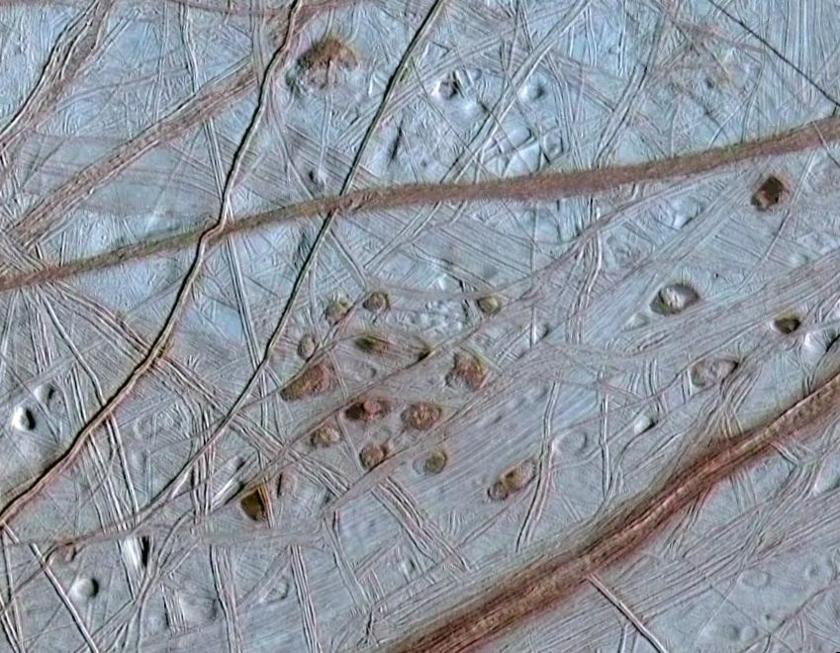
\includegraphics[scale=0.3]{figures/Orbiter/lenticulae.jpg}
    \caption{Lenticulae on Europa's surface / Courtesy of Galileo Project, NASA}
    \label{fig:lenticulae}
\end{figure}
\section{Chaos regions}
About one quarter of Europa’s surface is covered by highly disrupted areas mostly known as chaotic regions.  Most of these chaotic regions are concentrated in two oval shaped areas within 40$^{\circ}$ of the equator and centred at 120$^{\circ}$ and 300$^{\circ}$ W probably because these areas correspond to the location of paleopoles before the reorientation event, where tidal heating is more active. Also regions like Thera Macula, a low lying area with possible subsurface water, provide an indication of present active chaotic formation. Morphologically, chaos regions can vary presenting distinct characteristics or even combinations of them.

Plates of preexisting terrain are characterised by a spanning between 1-20km across, usually elevated from the surrounding area or with one of their edges tilted. Reconstruction models have shown that most of these plates have moved from their original positions, with 22\% of them showing a movement of over 5km. Other areas present inward facing scarps, slopes extending upwards into their neighbour terrain or even signs of chaotic terrain flowing into nearby ridges.
Numerous existing models have tried to describe the geophysical process of formation of these regions with the melting through the icy shell and brine mobilization models being the predominant, managing to explain most of the key and secondary observations. Melting through the icy shell model suggests that heat originating from the seafloor manages to melt the ice crust creating pits beneath the surface ice, while brine mobilization includes materials with low melting point conducting heat within the ice, lowering its viscosity and allowing leakage of liquids through the shell. Other models propose exogenic impacts on the surface as a mechanism of chaos region creation, while rising diapirs may be used to explain some large dome features.  
\begin{figure}[htb]
    \centering
    \includegraphics[scale=0.3]{figures/Orbiter/chaos.png}
    \caption{Conamara Chaos, Galileo E6ESBRTPLN01 observation \cite{chaosterrain}}
    \label{fig:conamara_chaos}
\end{figure}
Something that characterize the surface of these regions, is their distinctive dark red-brown color. Origin and exact composition of the material present on these area is still under investigation since not enough data are available but some estimations predict that probably is originating from sulfur compounds produced via radiolysis on the surface. Additionally spectral analysis of the same region on the infrared spectra, indicates the presence of a hydrated material like sulfate salts or sulfuric acid hydrate. If this estimation is confirmed then the low melting point of these materials, compared to the one of pure water ice, adds an important aspect in the formation of the chaos regions.
%\begin{itemize}
%    \item Avoid certain areas (brown areas, chemical compositions)
%\end{itemize}
%\todo[inline]{Resolution provided by current imaging from casini and imaging spectrometers?}
%\todo[inline]{Is 30 percent a realistic coverage? Why? Give a rough estimate of the suitable landing zones. }


\chapter{Orbiter and Imaging System}
\section{Introduction}
\todo[inline]{Introduction to the Europa Moon Surface/environment}
\todo[inline]{Brief Purpose of the Reconnaissance Imaging System}
\todo[inline]{Define limits and boundaries (the whole orbiter will not be designed)}
\section{Analysis of ERIS}
%\section{Analysis of the Imaging System}
The Europa Reconnaissance Imaging System (ERIS) plays an important role in the first phases of the mission. During the early stages, the imaging system will be used to map the surface of Europa and provide the necessary data for selecting a suitable landing site for the lander and penetrator. At this point, it is expected to have one or more cameras on the orbiter, mapping the surface of Europa in both low and high resolution. 
%\section{The Strawman Mission}
\subsection{The purpose of ERIS}
The Imaging System will be located in the orbiter, performing its primary objectives during the early stages of the life finding mission mission and performing the secondary objectives after a successful landing on Europa.

It is expected that the imaging system will be the main (and only) source of up-to-date, high resolution images before the actual landing. Therefore, it will be the only provider of the data that can be used for selecting a suitable landing site for the Europa Lander. It is assumed, that the current images provided from the Galileo Missions does not provide a high enough resolution to select a suitable landing site. This is the main reason why the relatively costly imaging system is required to perform mapping of the surface. 
%\todo[inline]{Provide source for this assumption, i.e. the resolution is too low using the sources from Galileo. Image examples?}
\subsection{Landing Site Selection}
During the first phase of the mission, the Imaging System will map the surface. The purpose of the mapping is to provide enough information about the surface, to ensure a suitable landing site can be selected and to ensure the landing will be successful. When selecting the landing site, the following criteria will be considered:
\begin{description}
    \item[Roughness and Elevation] The roughness of the surface can be a great danger for the lander. Large boulders can be fatal, blocking the penetrator from touching the ice or causing misalignment. Boulders can also cause the lander to flip, after an otherwise successful landing. Surface elevation is also very dangerous for the mission - too steep, and the lander can topple over, ending the mission immediately. Therefore, it is necessary to investigate technologies, that can be used to map the surface in high resolution, ensuring large objects can be identified and avoided, making it possible to land on a relatively flat surface.
    
    While high resolution imaging will make it possible to identify dangerous objects, it may not be possible to create topographic data of the lunar surface, unless the cameras are operated in stereo. Therefore, these technologies will also be investigated.
    \item[Radiation] Some areas of the moon have a lower radiation, making them more suitable for the landing site. These areas were discussed previously, in section (\ref{sec:radiation_environment}).
    \item[Chemistry] The current knowledge about the surface chemistry of Europa is very limited. However, spectroscopic data from the Galileo NIMS spectrometer hints that sulphur-rich regions exists. To investigate the surface chemistry, multispectral imaging should be investigated further, as it can provide data about the surface composition of Europa. Knowledge about the surface chemistry is necessary, as some regions may be very unsuited for a landing site, due to the hazardous chemical compounds that are expected in these areas (see section \ref{ch:surf_env}).
    %\todo[inline]{Refer to the previous section about surface composition. }
    \item[Proximity to ocean] Naturally, the selected landing site should be close to the ocean, as it is expected that the ice thickness (and therefore mission duration) will vary, depending on the selected landing site.
    
    Ice sounding radars are normally used for assessing the ice structure but this analysis will focus on technologies, that can be used to enhance the imaging system. Recent papers suggest that spectroscopic imaging can also be used for analysing the ice surface \cite{naegeli2015a} in addition to surface material assessment. However, this technique will likely be limited to a surface assessment - not a structural analysis of the ice.
    %\item[Communication window] The communication window will be affected by the choice of landing site b.
    %\todo[inline]{Communication Window. more to add Ifikratis}
\end{description}
\subsection{Manual vs. Automatic selection}
Due to the limited bandwidth, it is not realistic to transmit all the high resolution images back to earth, before the lander has made it to the surface. Instead, a selective approach will used, where all low resolution images will be transmitted to earth but only the regions of interests (ROIs) will be transmitted in back in high resolution. It is expected that the high resolution imaging will require a large amount of on-board storage. A large part of the available communication link capacity will also be required. At this point, the specific requirements are not known but estimates will be calculated later in this analysis.

Depending on the processing power available for the imaging system, it could be possible to perform an autonomous selection of the landing site. However, due to the lack of knowledge about the lunar surface at this point, it will be very difficult to design a selection algorithm beforehand. Relying on a fully autonomous system is not commonly done in the industry and creates an unnecessary risk for the whole mission. The alternative, a manual selection, is not difficult to implement, but requires two way communication to the spacecraft. The analysis will focus on providing the necessary data for a manual landing site selection but autonomous systems may still be useful to select and filter irrelevant images. The autonomous approach has been investigated briefly, as it can be a way to reduce the load on the communication and storage system (see section \ref{sec:aut_landing}).

For the landing site selection, the following approach is expected at this point: First, the ROIs are identified manually, using the low resolution images provided by the wide angle camera (WAC). By transmitting the low resolution images down to earth, it is possible for the ground station to select the ROIs, then instruct the spacecraft to transmit the stored high resolution imaging provided by the the narrow angle camera (NAC), as soon as a communication window opens.
%instruct the spacecraft to investigate these areas further, using the narrow angle camera (NAC).
It is not planned to dynamically change the flyby trajectory to investigate some areas further. Instead, both the WAC and the NAC will be operating during each flyby but only the WAC images will be transmitted down to earth, whereas the NAC images will be stored until the ground station requests higher resolution images of specific zones. By using the selective approach, only the relevant data will be transmitted, avoiding excessive load of the communication link.

It is expected that minimum 30\% of the lunar surface must be mapped, using the low resolution. This should provide the scientists with enough data to select several regions of interests, ultimately selecting a suitable landing site. The remaining 70\% of the lunar surface is expected to be unsuited for the landing site, based on the  current knowledge about the surface.
\subsection{Navigation - Orbit Determination}
As a secondary objective, the imaging system should provide data for the orbit determination required by the orbiter. Using the imaging system for both mapping and for tracking could be possible, but it may be difficult to do it at the same time. 

Orbit determination covers the task of continuously keeping track of the the position, where the spacecraft has been (orbit reconstruction), and where the spacecraft will be in the future (orbit prediction)\cite{doody2011spacefl} to ensure the spacecraft follows the required trajectory. Since the orbiter will be equipped with several imaging instruments, they can be used to observe planets or satellites together with the star field. This method provides the so called opnav images\cite{doody2011spacefl}. The images provide accurate and essential data about the trajectory of the spacecraft.  %Often, the primary body such as Europa will be overexposed, ensuring the background star field will still be visible. %The images will then be transmitted together with the rest of the telemetry data. 

Being able to track the spacecraft and predict the movement is certainly required for an interplanetary mission. Predicting the location of the spacecraft also makes it possible for the deep space network (DSN) to follow the spacecraft, ensuring stable communication throughout the mission. The navigational data are essential for the on-board systems, as they provide the flight path control system with the necessary data to successfully bring the spacecraft back on course, if it is deviating from the planned trajectory. The spacecraft will be drifting away from the planned trajectory, due to different disturbances encountered during the flight. Over a long distance, small disturbances will add up over time, causing a significant drift for the spacecraft. It is also important to keep in mind that trajectory corrections will never be perfect. A small misalignment of the thrusters or a delayed cut-off of the engines will all contribute to the trajectory drifts. %Depending on the choice of surface mapping technique, the drifts may severely affect the resulting images. 

Orbit reconstruction is essential to make sense of the scientific data collected by the spacecraft - including, but not limited to the data produced by the image system. The timestamps for the collected data and images must be paired with reference data such as the trajectory and orientation, to be able to perform a landing at a specific location or to use the data for scientific purposes. Most imaging techniques relies on very accurate knowledge about the trajectory, to be able to stitch the images together.
\subsection{Geo-localisation and Lander Guidance}
As an extra objective, the Imaging System will monitor the lander and provide geolocation and guidance services for the landing team. It is expected that the lander will not land exactly where it was initially planned. While interplanetary navigation has improved, it is still not perfect\cite{nasa2012}. Therefore, it should be possible to use the imaging system to locate the lander, after a successful landing. Knowing the final landing site is essential to ensure a successful communication link and to supervise the mission from the ground.
\section{Implementation of ERIS}
\section{Implementation of the Imaging System}
What is required to select a suitable landing site? What are the main objectives of the Imaging System? How does the physical properties of the orbiter limit the design? The answers to these questions define the initial system requirements for the design.
%\subsection{Selecting a suitable landing site}
\subsection{System Objectives}
To successfully select a landing site, it is necessary to gather more information about the lunar surface of Europa. This objective leads to a set of image system requirements.
\begin{description}
\item[Resolution]
The resolution for the WAC must be high enough that it is possible to identify ROIs. Based on \todo[inline]{Ifikratis image resolution analysis}, a resolution of 100 meters per pixel MPP is expected to be adequate for the worst case resolution, i.e. the resolution at the far operating distance. This defines the requirement for the WAC. The WAC will be producing the low resolution images used for the initial analysis and ROI selection.

When investigating the individual ROIs, it is expected that objects around the size of the lander (and larger) will pose a danger to the lander and must therefore be avoided. Assuming the lander will be around 1 meter in diameter \todo[inline]{Source for this assumption (refer to lander team specifications)}, the smallest feature that must be detected must be 1 meter. Referring to \cite{andor2016}, \cite{ni2014} and \cite{sbig2014}, a minimum of two pixels per smallest feature is necessary, to make an accurate measurement on the image. This defines the required resolution of 0.5 MPP for the NAC.

It is expected that a high enough resolution will make it possible to detect most surface roughness and elevation. However, if a detailed topographic mapping of the surface is necessary, it may be needed to operate the imaging system in stereo or to use additional instruments. Stereo imaging does not necessarily require two cameras. Instead, the movement of the spacecraft can be used to obtain images from two different angles, resulting in a stereo image. 
\item[Surface Chemistry]
The surface chemistry should be analysed, as some areas on Europa may be unsuitable due to the chemical compounds. One relatively simple way to enhance the imaging system is to add a selection of filters to the imaging system, making it possible to observe the radiance at different wavelengths. Ultimately, a spectra can be created of a given area. The spectra can later be analysed and compared to known chemical compounds. The higher the number of spectral bands, the more accurate the surface chemistry can be assessed. This type of enhancement is a good way to enhance an existing system, sharing the existing resources and costs, while providing additional capabilities to the orbiter.
%Adding imaging spectrometer capabilities to the imaging system is one way to enhance an existing system to provide extra functionality, without adding extra instruments.
%make it possible to assess the surface chemistry, while sharing the existing resources. using the capabilities of  without adding extra instruments.
\item[Ice surface Assessment]
In addition to the assessment of the surface chemistry, the ice surface must be analysed. Knowledge about the ice surface should make it possible to select a clean ice surface, with less gravel or dust. Since the proposed penetrator relies on melting the ice, inhomogeneous ice may cause the hole to clog with particles, bringing the melting process to a standstill. It is expected that the icy surface will not be homogeneous, based on the analysis in section (\ref{sec:lenticulae}). However, some zones may be dirtier than others, and will be unsuited as a landing site. Being able to differentiate between ice types will be a great help when selecting suitable landing sites. A recent study \cite{naegeli2015a} proposed the use of imaging spectroscopy for assessing the ice surface composition. The results from this study suggests imaging spectroscopy could be a good solution to differentiate between a range of different ice types.
\end{description}
\subsection{Mission Constraints}
The main objectives of the mission to Europa is to look for life and surveying plays a smaller role in the mission. The majority of the instruments included on the spacecraft will be used to look for life but this does not include the imaging system. Therefore, the mass, volume and power allocated for this system will be constrained.

However, without an imaging system on the orbiter, it will not be realistic to land on Europa. The existing images and knowledge about the surface is too limited, expressing the need for additional surveying beforehand. The system is therefore necessary but must be focused on providing mission critical data. It is also preferred if the support systems required by the imaging system can be shared with the remaining systems. Without any cost sharing, it is doubtful that the remaining mission teams will be supportive of the imaging system.
\subsection{Orbit Constraints}
The coverage that can be provided by the imaging system will be limited by the choice of orbit. When designing the telescopes and cameras, it is also crucial to have knowledge about the working distance of the imaging system. Therefore, the orbits must be planned in detail to ensure adequate coverage can be achieved and that the imaging system will be operating within suitable ranges.

The choice of orbit may also affect the lifetime of the imaging system, as the radiation environment varies greatly. Naturally, this will also affect the required radiation shielding and the mass and volume requirements.
\todo[inline]{More to add about orbit constraints? Radiation?}
\subsection{Alignment and Calibration}
\todo[inline]{Implementation: Include ways to calibrate, align spacecraft/telescope}
\newpage
\section{System Overview}
Due to the complexity of the imaging system, the system will be split in individual subsystems. For each subsystem, a set of solutions will be proposed. First, the overall structure of the image system will be defined, creating the framework for the proposed imaging system.
\subsection{Imaging System Structure}
When selecting the structure, the first question is the number of cameras that should be used. Mapping and surveying Europa is not the primary goal of the mission but is necessary to gain prior knowledge, before the landing can begin. Therefore, the allocated resources for the imaging system will limited.

Naturally, a single camera would limit the required resources but would also limit the tasks that can be completed by the imaging system. A camera can be designed as a wide angle camera (WAC) or narrow angle camera (NAC) - but not both. The WAC would be very useful for the identification of ROIs, as this phase requires a large surface coverage in relatively few flybys. The large field of view (FOV) of the WAC means a large surface area can be covered, but in a low resolution. In contrast, the NAC would be very suitable for the high resolution imaging of interesting regions but would require many flybys to achieve a high enough coverage of the surface.

Since the imaging system does not have top priority in this mission, it is important to consider how the system can provide useful data for the remaining groups. Having a WAC is very useful for the orbit determination, as it will be suitable for observing a large planet or satellite together with the background star field, providing the opnav images used for orbit determination. Having both a WAC and a NAC is also very useful for the lander guidance objective and geolocation. The "global" mapping can be provided by the WAC whereas the "local" mapping can be provided by the NAC. By correlating the two image sets, geo-localisation in both high and low resolution is possible.

Tracking a fast moving object with a NAC can be very difficult, as the object can easily move outside the camera frame - causing a loss of tracking. A WAC makes it possible to track the lander, without requiring a high pointing accuracy. As long as the camera is pointing in the general direction of the lander, it will be within the camera frame.

Another important aspect to consider is the redundancy of the camera system. Naturally, having duplicate systems available will be preferred, if one system fails. One type of redundancy is to have an identical camera on standby but this will require a larger allocation of resources for a system, that may not be necessary, unless a camera actually fails. A different approach is to bring both a NAC and WAC. While each camera is suited for a specific task, they can substitute each other to a degree, if one camera fails. However, the performance of the image system will be degraded, depending on which camera that fails. The WAC is the most irreplaceable one of the cameras, as it will not be possible to cover a large enough surface area, if this camera fails. This will in turn require many more flybys to obtain adequate coverage - prolonging the mission.

The WAC can operate on its own, but it will require a dynamic flyby to re-target a specific region of interest. After covering the area in low resolution, it will be necessary to cover the area again, using a higher resolution (and therefore a lower altitude). The WAC can only provide an adequate resolution, if the orbiter passes closer to Europa. 

When considering a camera system that should generate data about the surface elevation, it is natural to consider stereo imaging. The common way to generate stereo images is to operate two cameras at once, each viewing the scene from a slightly different angle. As this is a costly approach, an alternative way is proposed for this mission. By using the spacecraft attitude control systems to move the spacecraft, it is possible to generate stereo images, using only one camera. This method is illustrated in figure \ref{fig:stereoimg}. Naturally, it will require more from the attitude control systems, as the spacecraft must be able to point in specific directions on command. However, using this approach, stereo imaging can be added - independent on the number of cameras provided by the orbiter.

\begin{figure}[h!]
\centering
\includegraphics[width=0.4\textwidth]{figures/Orbiter/Stereo_Satellite.png}
\caption{Stereo Imaging using one camera. Source: DigitalGlobe, \cite{satimgcorp2015}.}
\label{fig:stereoimg}
\end{figure}

The two structures are compared in table (\ref{tab:score_system_structure}). It is apparent that the single camera method is a simple and cheap but it will be less suited for a surface mapping, as it can only provide either wide or narrow angle imaging - but not both. As the WAC is the most flexible camera of the two, it has been selected as the camera used for the single camera method. While it may be possible to fulfil all objectives using only one WAC, it will increase the complexity of the flyby and will require multiple passes - one for the low and one for the high resolution. The limited flexibility for the single camera is also the main reason why it will be performing poorly at all of the secondary objectives.
\begin{table}[h!]
  \centering
    \begin{tabular}{l|l|rr}
    \multicolumn{2}{c|}{\textit{\textbf{System Structure}}} & \textit{Single (WAC)} & \textit{Dual (WAC + NAC)} \bigstrut[b]\\
    \hline
    \textbf{Design Drivers:} & \textit{Simplicity} & 5     & 3 \bigstrut[t]\\
          & \textit{Flexibility} & 1     & 5 \\
          & \textit{Physical Req.} & 5     & 3 \\
          & \textit{Support System Req.} & 4     & 2 \\
          & \textit{Orbit} & 1     & 5 \\
          & \textit{Redundancy} & 1     & 2 \bigstrut[b]\\
    \hline
    \textbf{Primary:} & \textit{Surface Mapping} & 1     & 5 \bigstrut\\
    \hline
    \textbf{Secondary:} & \textit{Orbit Determination} & 3     & 5 \bigstrut[t]\\
          & \textit{Geo-location} & 3     & 5 \\
          & \textit{Topography} & 4     & 4 \bigstrut[b]\\
    \hline
    \multicolumn{1}{l}{\textbf{Total:}} & \textit{\textbf{}} & 28/50 & 39/50 \bigstrut[t]\\
    \end{tabular}%
  \caption{The score table for the Imaging System Structure. 5 is the highest grade given.}
  \label{tab:score_system_structure}%
\end{table}%

From the score table, it is easy to see that the overall performance will be better with the second approach. The dual camera approach will require more from the physical resources and the support systems. However, it performs well at both the primary and the secondary objectives and it performs the high and low resolution imaging at the same time, thus avoiding multiple flybys. In addition, it contains redundancy to a certain degree. If one camera fails, all objectives can still be completed but it will be at a lower performance as described earlier. If the WAC fails, it may be difficult to get a large enough coverage of the surface, due to the narrow field of view of the remaining camera. It will also require clever post-processing\footnote{Such as Image stitching, combined with averaging to create low resolution maps from the high resolution imaging.} of the high resolution images, to make up for the lack of surface coverage. If the NAC fails, it will be more complicated to provide high resolution imaging, due to the small focal length of the WAC. In this case, it will be necessary to operate the WAC at a lower altitude.

To improve the redundancy and the reliability of the system structure, an extra WAC should be included in the design, as this is the most important and smallest camera\footnote{The WAC is assumed to be small, due to the relatively small focal length} of the two. It could even be operated together with the primary WAC, to increase the surface coverage or to capture stereo imaging. The NAC is also important, as it makes it possible to generate high resolution images at the same time as the WAC operates. However, due to physical constraints, it is not possible to bring two complete telescope\footnote{Due to the large focal length required by the NAC, a telescope is assumed.} assemblies. As an alternative, multiple detectors can be added to the telescope, making it possible to switch if one detector fails. As it is most likely that only the detector will fail due to the radiation and not the telescope, this is a good and efficient solution to the redundancy problem. 
\subsection{Telescope and Sensor}
Telescopes/lens that will be considered for the camera system. 
\todo[inline]{Suggested telescope types based on LROC, LORRI, ISS (Ifikratis)}
\subsection{Sensor}
\todo[inline]{Suggested sensor types (Ifikratis)}
When selecting the sensor for the camera, there are several factors that must be considered\cite{sbig2014}. 
\todo[inline]{http://www.astro-imaging.com/Tutorial/MatchingCCD.html}
\begin{description}
\item[Field of View] The WAC and the NAC will require a specific field of view (FOV), as the purpose for the cameras are different. The field of view that will be seen by the camera is determined by the physical size of the sensor and the focal length of the telescope. A larger sensor will have a larger field of view, at a given focal length. If the FOV is kept fixed, a large sensor will require a larger focal length to maintain the FOV. This will require a larger lens or telescope\cite{sbig2014}. 

The focal length affects the physical requirements of the design and should therefore be as small as possible. It is preferred to select a sensor size, that will result in the smallest possible focal length.
\item[Sensitivity] The sensitivity of the sensor is determined by several factors; the pixel size and quantum efficiency\cite{sbig2014}. The quantum efficiency (QE) of the sensor measures how efficient the photons are converted into electrons. A higher QE will result in a greater sensitivity and the sensor will therefore require less time to capture an image, when compared to a sensor with a lower QE\footnote{Assuming an equal signal to noise.}. The efficiency is usually dependent on the wavelength. As each sensor is designed for a specific task, a sensor designed for capturing visible light (and preferably reject any other wavelengths) will not be very useful for an imaging spectrometer, operating outside the visible range. It is therefore important to verify the working range for the sensor.
\item[Resolution and Pixel Size]
It is also important to consider the pixel size for the sensor. If the pixels are too small, the object will be sampled with more pixels than necessary (oversampling). If the pixel is too big, the image will fall within the pixel\footnote{Assuming a projected image, with a diameter smaller than the pixel size} and the sensor will reproduce the object as a 1 pixel square (undersampling). This problem is illustrated in figure \ref{fig:pix_size_compare}.
\begin{figure}[h]
\centering
\includegraphics[width=0.4\textwidth]{figures/Orbiter/pixel_size_compare.jpg}
\caption{The pixel size should be selected according to the projected image, \cite{andor2016}.}
\label{fig:pix_size_compare}
\end{figure}
If the object is slightly larger, it will still only be reproduced as a single pixel, with four slightly dim pixels surrounding it. However, when the image covers more than three pixels, the circular object is clearly reproduced. The goal is to sample the object with two to four pixels. This will give the best balance between sensitivity and resolution\cite{sbig2014}. Naturally, the actual object size will depend on the telescope focal length. Matching the sensor pixel size and the focal length will therefore be essential to get high enough sensitivity, without sacrificing resolution.
\item[Speed]
\todo[inline]{readout speed, as required by the calculations}
\item[Dark Current]
\item[Rad-hard]
\end{description}
\todo[inline]{Actual sensor selection...}
\subsection{Spacecraft Pointing and alignment}
\todo[inline]{Tip tilt mirror - top down imaging vs. rotating - coverage?}
\todo[inline]{Which types of camera "movement" will be used to get larger coverage? Tip Tilt? etc.}
\subsection{Imaging Spectroscopy}\label{sec:imaging_spectroscopy}
By combining conventional imaging with spectroscopy, it is possible to obtain both the spatial and spectral information of the lunar surface. This combination is commonly known as imaging spectroscopy. This is illustrated in figure \ref{fig:spectral_information}. In this illustration, the spectral bands has been separated using the white lines. Hyperspectral imaging uses many, relatively narrow bands. In comparison, multispectral imaging uses fewer, broader bands, resulting in a lower spectral resolution. 
\begin{figure}[H]
\centering
\includegraphics[width=0.75\textwidth]{figures/Orbiter/spectral_information}
\caption{The resolution is defined by the number of bands but also by their bandwidth.}
\label{fig:spectral_information}
\end{figure}
The usefulness of the spectroscopic data depends on the spectral resolution\cite{elowitz2016}. Multispectral imaging makes it possible to detect the presence of simple classes such as vegetation, water and so on. It provides limited information about the actual surface materials. On the other hand, hyperspectral imaging makes it possible to identify surface features, based on the unique spectral signature and thus determine the surface materials, as long as the spectral signature matches an already known substance from the databases. In some cases, it may also be possible to determine subtypes of the materials, such as dirty or clean ice, snow etc\cite{naegeli2015a}. Some materials, such as icy surfaces will have their \textit{spectral fingerprint} within the visible light domain whereas other materials must be observed in the near IR or IR domain to be accurately identified.

Common RGB (color) cameras detects radiation in three bands, typically blue (400 - 470 nm), green (480 - 550 nm) and red (570 - 700 nm) whereas multi- or hyperspectral cameras can acquire images at many more bands, either by adding a spectral dispersion element or filter to the camera\cite{crisp2001}. 
\subsubsection*{Multispectral Imaging}
This type only uses a few extra bands, in addition to the basic color bands (RGB). Around ten bands are commonly used for this imaging technique\cite{elowitz2016}.

One way to implement a simple multispectral camera is to use a filter wheel in front of the detector, illustrated in figure (\ref{fig:filtwheel_miri}). As the selected filter covers the whole detector, the complete image will be filtered and captured. Different filters can be applied in a sequence, effectively creating multispectral data of the lunar surface. 
\begin{figure}[H]
\centering
\includegraphics[width=0.30\textwidth]{figures/Orbiter/miri_filterwheel.jpg}
\caption{The filter wheel used for the MIRI instrument onboard the James Webb Space Telescope. Source: MPIA}
\label{fig:filtwheel_miri}
\end{figure}
%\todo[inline]{is it relevant to include this image?}
As the spectral data will be arranged in full frames, only simple post-processing is required to group the spectral "sheets" together, before they are transmitted. However, the filter wheel introduces moving parts, adding to the total weight and complexity of the system. The number of spectral bands will be limited, due to the available space on the wheel. More than 20 bands are not common using this method. Due to the limited number of bands, multispectral imaging will not generate a continuous spectrum but instead generates discrete spectral bands. As the spectral resolution is limited, the usability of the spectral data will be limited as well.

It is important to keep in mind that this method will require additional time when switching between each filter. Due to this delay, each frame may be slightly misaligned, due to the spacecraft movement between frames.
\subsubsection*{Hyperspectral Imaging}
Most imaging spectrometers rely on complex optical systems to split the light into continuous, narrow bands. This includes the Fourier spectrometer and the grating spectrometer. The wedge spectrometer has been proposed in \cite{puschell1999a} as a simpler alternative. By comparing the different spectrometer assemblies in figure (\ref{fig:spec_compare}), the simplicity of the wedge spectrometer is obvious. Due to the limited time available in this course, the Fourier Transform spectrometer has not been analysed further.
\begin{figure}[H]
    \centering
    \begin{subfigure}[b]{0.3\textwidth}
        \includegraphics[width=\textwidth]{figures/Orbiter/spectrometer_fourier.png}
        \caption{Fourier Transform}\label{fig:spec_fourer}
    \end{subfigure}
    \begin{subfigure}[b]{0.3\textwidth}
        \includegraphics[width=\textwidth]{figures/Orbiter/spectrometer_grating.png}
        \caption{Grating}\label{fig:spec_grating}
    \end{subfigure}
    \begin{subfigure}[b]{0.3\textwidth}
        \includegraphics[width=\textwidth]{figures/Orbiter/spectrometer_wedge.png}
        \caption{Wedge}\label{fig:spec_wedge}
    \end{subfigure}
    \caption{A comparison between spectrometer types. Source:\cite{puschell1999a}.}\label{fig:spec_compare}
\end{figure}
The Wedge Imaging Spectrometer could be a suitable candidate for the system, as it will certainly require much less mass than the alternatives while providing better spectral resolution, compared to the simple filter wheel approach. Filter based spectrometers, such as the wedge type (\ref{fig:spec_wedge_acq}) uses a linear variable filter (LVF), where the spectral properties vary linearly on the wedge\cite{joseph2015building}. The filter is constructed by overlaying layers of dielectric film with high and low refractive indexes in a specific pattern. Because of the tapered dielectric coatings of the film, the passband center wavelength for the thin-film stack will essentially depend on the thickness of the stack. Therefore, the center wavelength of the radiation passing through the wedge filter will vary linearly along the tapered edge of the wedge filter\cite{joseph2015building}. This concept is illustrated in figure (\ref{fig:spec_wedge2}).
\begin{figure}[H]
\centering
\includegraphics[width=0.65\textwidth]{figures/Orbiter/spectrometer_wedge_3}
\caption{The Linear Wedge Filter, mounted on the detector. Adapted from:\cite{puschell1999a}.}
\label{fig:spec_wedge2}
\end{figure}
From the figure, it can be seen how the wedge filter is coupled very close to a 2D detector array, with the coated surface facing the array. A blocking filter, covering the spectral region of interest is mounted on the opposite side of the substrate, to remove out-of-band radiation. Each detector row in the spatial dimension is aligned with a given spectral band, using an even spacing between each band. Therefore, the rows will receive light at different wavelengths.

The filter wheel requires several moving parts and a therefore a larger mass. However, it offers an increased amount of flexibility as the system can easily operate with or without filters applied to the imaging sensor. This makes the method very suitable for the secondary objectives, where a filter is not strictly necessary.

The Grating Spectrometer offers a much higher spectral resolution but is unsuited due to the complex design. It is also not very flexible, as it will not be possible to operate the system without generating spectral data, making it unsuited for the secondary objectives. Due to the limited image acquisition methods possible, it will also not be able to give adequate coverage. The different imaging spectrometers has been compared in table \ref{tab:score_imaging_spectrometer}. 
\begin{table}[H]
  \centering
\begin{tabular}{l|l|rrr}
\multicolumn{2}{c|}{\textit{\textbf{Imaging Spectroscopy}}} & \textit{Filter Wheel} & \textit{Grating} & \textit{Wedge} \bigstrut[b]\\
\hline
\textbf{Design Drivers:} & \textit{Simplicity} & 3     & 2     & 5 \bigstrut[t]\\
      & \textit{Flexibility} & 4     & 2     & 3 \\
      & \textit{Physical Req.} & 2     & 2     & 5 \\
      & \textit{Support System Req.} & 3     & 2     & 2 \\
      & \textit{Processing Req.} & 5     & 3     & 3 \\
      & \textit{Redundancy} & 2     & 1     & 4 \bigstrut[b]\\
\hline
\textbf{Primary:} & \textit{Spectral Resolution} & 1     & 5     & 5 \bigstrut[t]\\
\textbf{} & \textit{Coverage} & 3     & 2     & 4 \bigstrut[b]\\
\hline
\textbf{Secondary} & \textit{Orbit Determination} & 4     & 1     & 3 \bigstrut[t]\\
      & \textit{Geo-location} & 4     & 1     & 3 \\
      & \textit{Topography} & 4     & 1     & 3 \bigstrut[b]\\
\hline
\multicolumn{1}{r}{\textbf{Total:}} & \textit{} & 35/55 & 22/55 & 40/55 \bigstrut[t]\\
\end{tabular}%
  \caption{The score table for the Imaging Spectrometer. 5 is the highest grade given.}
  \label{tab:score_imaging_spectrometer}%
\end{table}%
The wedge spectrometer scores slightly better than the filter wheel method. The system trades higher processing requirements and higher support system requirements with a very simple and relatively flexible system. Processing power is relatively cheap on the spacecraft but the higher requirements from the support systems, such as the attitude control, will be the main challenge with this design. However, this is to be expected, when performing surface imaging.

A high spectral resolution and good coverage is possible with the wedge spectrometer but it can be seen how the system performs slightly worse at the secondary objectives. This is caused by the limitations of the wedge filter, as it can only capture an image frame by scanning, operating as a push broom imager. The push broom technique is not very suitable for capturing opnav images or topographic images.

To improve the performance, a simple solution is suggested. By having an extra detector, the wedge filter and sensor assembly can be removed from the telescope and switched with a bare detector. If a 2D detector is used, this makes it possible to capture full frame images with no filter applied. While it will require moving parts, it will greatly improve the performance of the non-spectral imaging capabilities of the system.
\subsubsection*{Image Acquisition}
When considering what spectrometer to use for the imaging system, it is not just a  matter of selecting the lightest and simplest design. Examining the assembly of the two different spectrometer systems makes it clear how the images will be acquired and how the output data will be ordered. The image acquisition method is important to consider, as the ordering of the generated data can affect the post-processing system significantly. Common methods include whisk-broom/push-broom (pixel or line) or staring (frame) captures. The two spectrometer assemblies are shown in figure (\ref{fig:spec_acquisition_compare}). 
\begin{figure}[H]
    \centering
    \begin{subfigure}[b]{0.45\textwidth}
        \includegraphics[width=\textwidth]{figures/Orbiter/spectrometer_colli_nieke.jpg}
        \caption{Dispersive Type}\label{fig:spec_dispersion_acq}
    \end{subfigure}
    \begin{subfigure}[b]{0.45\textwidth}
        \includegraphics[width=\textwidth]{figures/Orbiter/spectrometer_wedge_nieke}
        \caption{Wedge Filter Type}\label{fig:spec_wedge_acq}
    \end{subfigure}
    \caption{A comparison between acquisition methods. Adapted from:\cite{nieke1997a}.}\label{fig:spec_acquisition_compare}
\end{figure}
The first method (\ref{fig:spec_dispersion_acq}) uses gratings or prisms as the dispersion element. The element separates the incoming electromagnetic radiation into different wavelengths. A single ground pixel is dispersed and focused onto different locations on the array detector\cite{nieke1997a}, resulting in a whisk-broom acquisition but with each "whisk" covering a specific spectral band. This

The wedge spectrometer is realised by mounting the detector filter assembly in the focal plane of the imaging optics (\ref{fig:spec_wedge_acq}), \cite{joseph2015building} and \cite{nieke1997a}. By placing the wedge filter along the direction of movement, the imaging system is able able to capture a frame of each cross strip from $x_1$ to $x_n$. With With $n$ strips covering different surface areas, each cross strip will correspond to a specific spectral band, depending on the region on the wedge filter. If a 1D array detector is used (i.e a detector that is 1 pixel wide), the spectrometer will be acquiring each spectral band in a whisk-broom fashion. By using a 2D array detector instead, the spectrometer will acquire the spectral bands in a push-broom fashion. Each recorded frame will contain $n$ different ground strips corresponding to each of the spectral bands in the filter. When the spacecraft moves, each ground strip will be imaged by different positions on the wedge filter, thus creating multispectral data for each surface area.

Unlike the dispersive type, where the full spectra of a single pixel is recorded in a single frame, the wedge filter requires reorganising the data, before the hyperspectral cube can be generated for a given surface area. With $n$ spectral bands, the first and the last band for a given ground strip will be collected with a time difference of $(n-1)\cdot \tau$. As the spectral bands for each ground strip will not be linked, the the attitude stability of the spacecraft will therefore play a major role in the band-to-band registration accuracy\cite{joseph2015building}, therefore requiring more from the support systems. The wedge filter imaging sequence is illustrated in figure (\ref{fig:wedge_filt_img_sequence}), where the surface area is illustrated by the blue square.
\begin{figure}[H]
\centering
\includegraphics[width=\textwidth]{figures/Orbiter/wedge_filt_img_sequence.pdf}
\caption{The wedge filter imaging sequence. Adapted from:\cite{joseph2015building}.}
\label{fig:wedge_filt_img_sequence}
\end{figure}

At time $T$, the ground area will be viewed by channel $\lambda_7$, at $T+\tau$ the area is viewed by channel $\lambda_6$ and so on. Therefore, it is necessary to use post-processing to link the spectral data together. As the raw data cannot be transmitted due to communication constraints, they must be processed and reordered on the spacecraft. A large part of the image system is therefore to design an efficient and fast processing system that can process and store the images faster than they are generated.

When operating the spectrometer as a push-broom imager, a large amount of data will be generated. Additionally, the dispersion spectrometer and the wedge spectrometer generates data in a different order, when compared to the simpler filter wheel method, apparent from figure (\ref{fig:wedge_filt_img_sequence}). Each section of the imaging sensor is dedicated to a specific spectral band. 

Unlike the full frame capture used by the filter wheel, the push-broom techniques generate all spectral data in parallel. With many parallel data streams, it is a problem very suitable for a parallel processing system, where each spectral data stream is computed individually.
\todo[inline]{other aspects to consider when designing hyperspectral cameras (see joseph2015building, page 272)}
\section{Imaging System Proposal}
The imaging system consists of several subsystems. Based on the previous analysis of each subsystem, the overall imaging system will now be specified.
\subsection{Imaging System Structure}
A dual camera system structure, using both a NAC and a WAC is proposed for the final design. The selected system structure requires a more complicated design but will make it possible to perform both the primary and secondary objectives at a high performance. As the surface imaging is not the primary mission objective, it is important that the system can provide useful data for the remaining groups.

The two cameras will be very suited for capturing both low and high resolution imaging at the same time. Some of the secondary objectives are better suited with the WAC (lander tracking and opnav imaging) whereas both cameras will be suited for the geolocation operation. The two cameras can substitute each other to a degree, providing built in redundancy. Therefore, the mission can still continue, if one camera fails. However, as the WAC is complicated to replace, it is suggested that a secondary WAC is included as a backup. Operating the primary and secondary WAC together will also make it possible to increase the surface coverage and make it possible to generate stereographic images. 
\todo[inline]{diagram of the imaging system structure}
\subsection{Telescope and Detectors}
\todo[inline]{Which design has been selected for Telescope and Detectors and why?}
\subsection{Spacecraft Pointing and alignment}
\todo[inline]{Selecting the Final pointing method and argument for this selection}
\subsection{Imaging Spectroscopy and Acquisition}
Combining the suitable parts from both the filter wheel and the wedge spectrometer results in the proposed solution for this subsystem. The wedge filter provides the spectral data but can be removed from the sensor, making it possible to capture the full frame images suited for the secondary objectives. In this way, high performance is ensured for both the imaging and spectroscopy mode. 

The system design remains simple, but requires slightly more moving parts for switching the filter. However, it is the increased support system requirements (attitude control, processing and storage resources) that will drive the cost. Naturally, surface mapping using a high spectral resolution will require more from the support system and cannot be avoided. However, if the support systems are already required and will be shared, this will not be an issue.

Image acquisition can be done in two different ways, when using the wedge spectrometer - using whisk-broom or push-broom. The main difference is the coverage or swath\footnote{Swath; the width of the lines sweeping over the surface} per flyby. Naturally, a large coverage is required to minimise the number of flybys required, making push-broom a suitable image acquisition method. This approach will require a 2D
array detector, as each spectral channel has a matching area on the detector. The detector will capture a full frame at a time but the spectral data will be structured in individual areas on the detector. As the data are structured in this fashion, it is necessary to process and store the images, before they can be transmitted to the ground station.
\subsection{System Flaws}
\todo[inline]{System flaws? Is this the best solution?}
\subsection{Similar Systems}
\todo[inline]{Currently Available NAC/WAC - See powerpoint}
\todo[inline]{What changes will be necessary to adapt the current systems?}
\section{Support Systems Overview}
\todo[inline]{Required support systems. Other to add?}
The imaging system requires several support systems that will either be provided as part of the imaging system or shared between the other systems on the orbiter. A comparison of the cost drivers for the different support systems are shown in table \ref{tab:design_cost_driver}. Only a few of the support systems are not shared with other on-board instruments.
\begin{table}[h!]
  \centering
\begin{tabular}{p{4cm}|p{11cm}}
\toprule
      & \textbf{Design and cost drivers} \\
\midrule
\textit{Orbit Determination and Attitude Control} & Essential for navigation, accuracy required by imaging system \\
\textit{Image Processing} & Essential for imaging system \\
\textit{Generic Processing} & Generic processing power is essential for the orbiter. \\
\textit{Data Storage} & A large data storage is necessary for the imaging system but other systems will also require data storage. \\
\textit{Thermal Control} & Thermal control is crucial for the orbiter, especially due to the RTG. Thermal control is also essential for the imaging system. \\
\textit{Power System} & A power system must be present for both the imaging system and remaining systems. \\
\textit{Radiation Protection} & Radiation protection is essential for all electronics, including communication. Especially the detector (CCD) will require protection. \\
\bottomrule
\end{tabular}%
  \caption{Comparison of the design and cost drivers used by the orbiter.}
  \label{tab:design_cost_driver}%
\end{table}%
\subsection{Attitude Determination and Control}
To ensure the stability and achieve the correct orientation of the orbiter-spacecraft, a complete attitude determination and control system will be utilised. The four gravity assist flybys, along with the planned close encounters with Europa to determine a safe landing site using the optical sensors of the spacecraft, raise the requirements for high accuracy and reliability of the attitude subsystem.

Closest approach to Europa at a distance of 100km with a flyby speed of 3.3 km/s and an angular velocity of approximately 0,002rad/s (or 0,1146$^{\circ}$/s), sets the stearing and pointing accuracy requirements of the orbiter. 
% Table generated by Excel2LaTeX from sheet 'Sheet1'
\begin{table}[h!]
  \centering
    \begin{tabular}{|p{4,7 cm}|p{4,7 cm}|p{4,7 cm}|}
    \hline
    \textbf{Stearing} & \textbf{Effect on Spacecraft} & \textbf{Effect on ADC Selection} \bigstrut\\
    \hline
    Nominal rates 0,05 - 0,5 deg/sec & Minimal & Thrusters \bigstrut\\
\cline{3-3}          &       & Reaction wheels \bigstrut\\
    \hline
    \end{tabular}%
    \caption{Stearing requirements \cite {spacemissionanalysis}}
  \label{tab:stearing_req}%
\end{table}%

% Table generated by Excel2LaTeX from sheet 'Sheet2'
\begin{table}[h!]
  \centering
    \begin{tabular}{|p{4,7 cm}|p{4,7 cm}|p{4,7 cm}|}
    \hline
    \multicolumn{1}{|c|}{\textbf{Required Accuracy}} & \multicolumn{1}{c|}{\textbf{Effect on Spacecraft}} & \textbf{Effect on ADC Selection} \bigstrut\\
    \hline
          &       & Need for accurate attitude reference (Star Tracker $\mu$ASC) \bigstrut\\
\cline{3-3}    0,1 - 1 deg & 3-axis and momentum - bias stabilisation & Reaction wheels \bigstrut\\
\cline{3-3}          &       & Thrusters for momentum unloading and coarse control \bigstrut\\
    \hline
    \end{tabular}%
    \caption{Pointing accuracy requirements \cite {spacemissionanalysis}}
  \label{tab:point_acc_req}%
\end{table}%
Attitude determination will utilise a set of four micro-Advanced Stellar Compass ($\mu$ASC) star trackers (Table \ref{tab:masc}), while electrically-powered reaction wheels will be responsible for the 3-axis control. External disturbance torques will saturate eventually the wheel speed of the reaction wheels, so a set of gimballed thrusters are necessary for  momentum unloading ensuring attitude stabilisation.

% Table generated by Excel2LaTeX from sheet 'Sheet2'
\begin{table}[h!]
  \centering
    \begin{tabular}{|r|c|}
    \hline
    Initial acquisition & 30msec \bigstrut\\
    \hline
    \multicolumn{1}{|c|}{Accuracy} & 1” \bigstrut\\
    \hline
    \multicolumn{1}{|c|}{Attitude rate} & Up to 10$^{\circ}$ /sec \bigstrut\\
    \hline
    \multicolumn{1}{|c|}{Update rate} & Up to 20Hz \bigstrut\\
    \hline
    \multicolumn{1}{|c|}{Availability} & 99,995\% \bigstrut\\
    \hline
    \multicolumn{1}{|c|}{Power} & 1.9W \bigstrut\\
    \hline
    \multicolumn{1}{|c|}{Mass} & 425g \bigstrut\\
    \hline
    \multicolumn{1}{|c|}{Size} & DPU: 10x10x4.5cm CHU: 5x5x5cm \bigstrut\\
    \hline
    \multicolumn{1}{|c|}{Lifetime} & $>$30 years \bigstrut\\
    \hline
    \multicolumn{1}{|c|}{Reliability} & 99,999\% \bigstrut\\
    \hline
    \end{tabular}%
    \caption{$\mu$ASC star tracker specifications \cite {masc}}
  \label{tab:masc}%
\end{table}%
Selection of the proposed combination assures an autonomous and high accuracy pointing of the imaging system and the pointing of the high gain antenna toward Earth as well. 
\subsection*{Img...}
This sub system is required to make it possible for the surface imaging to follow a specific pattern, increasing the surface coverage. The accuracy of the attitude control is partially driven by the specific accuracy requirements by the imaging system. However, attitude control is a crucial part of the navigation and orbit determination. Attitude control is also required to maintain a stable communication link to the ground station. 

As previously suggested, the imaging system could be used to generate the opnav images used for orbit determination. Using the imaging system for both mapping and for tracking could be possible, but it may be difficult to do it at the same time. It may also require a different camera design, as both the relatively bright lunar surface and the dark star background must be possible to photograph.

If the imaging system cannot be used for both tasks, a separate orbit (and orientation) determination subsystem is required in addition to the imaging system. Naturally, actuators for correcting the trajectory will also be required for the attitude control. These support systems will be needed - with or without an imaging system, as they are an essential part of any spacecraft navigation system. Therefore, it is not expected that the imaging system will be driving the design requirements alone.
\subsection{On-board Processing and Data Management}
The imaging system requires a processing system to prepare the images, before they are transmitted. The system will filter and compress the data from the imaging system, only sending the instructed data down to the ground station. The communication window will be very short, limiting the amount of data that can be transmitted. Therefore, on-board storage is required. As the digital image processing system will most likely be a problem specific (ASIC or FPGA) implementation, it will only be useful for the imaging system and other specific problems such as data compression. On the other hand, the storage bank(s) can certainly be shared between the rest of the systems requiring a storage buffer between communication windows, as long as these systems do not require a huge data storage. Any other programmable processors required by the imaging system can also be shared with the other instruments on the orbiter.
\subsection{Thermal Management}
Thermal control of the spacecraft is essential, as it is required to ensure the electrical and mechanical parts of the imaging system will be operating within a specific temperature range\cite{fortescue2011a}. Often, the electrical and mechanical systems will only operate efficiently and reliably, if they are kept within this range. Often, the parts must be operated around room temperature. Most spacecraft originated as parts meant for terrestrial use and were therefore developed under this environment.

Most electronic systems, such as the microprocessors and power supply circuits should be operating in a temperature range of $-15^\circ$C to $+50^\circ$C. Mechanical mechanisms such as momentum wheels, gyroscopes and telescope shutters must be operated between $0^\circ$C to $+50^\circ$C and batteries between $0^\circ$C to $+20^\circ$C\cite{fortescue2011a}.

Thermal control is already required by the electrical communication hardware so the imaging system is not the only design and cost driver here. An advanced thermal system is also required to move the heat from the RTG away from the spacecraft, keeping the spacecraft from overheating. At the same time, a temperature difference across the peltier elements must be maintained, to generate power. 

However, the imaging system will require a very high structural stability to maintain high pointing accuracy. This means the thermally induced distortion must be minimised or controlled as part of the orbiter design. The CCD detector used in the cameras will also benefit greatly from a lower temperature. The thermal energy is enough to excite electrons into the image pixels, indistinguishable from actual photo-electrons. This event generates noise and is also known as \textit{dark current}. Fortunately, the dark current can be decreased if the CCD temperature is reduced. Typically, the dark current rate can be reduced by 50\%, if the CCD temperature is reduced by $6-7^\circ$C \cite{sbig2014}. For the KAF-8300 CCD mentioned in this source, the noise has almost disappeared, when the CCD is cooled to $-30^\circ$C. It is expected that a temperature between $-30^\circ$C to $-50^\circ$C would be a suitable choice but it depends on the specific CCD.
\todo[inline]{Specific CCD requirements}
\todo[inline]{Thermal system diagram?}
\newpage
\subsection{Power Systems}

Power system design utilises a single General Purpose Heat Source - Radioisotope Thermoelectric Generator (GPHS-RTG) Fig.\ref{fig:rtg}. The deep space nature and the multi-year duration of this mission, renders the use of an RTG necessary. At a 5.2 AU distance from the sun, selection of a solar PV-battery configuration is considered prohibited, taking into account the weak solar flux and the limited the mass budget. Furthermore, excess thermal power produced by the RTG can be exploited for the heating needs of the internal electronic components.


\subsubsection*{General Purpose Heat Source - RTG} 
Utilizing the natural decay of plutonium-238 oxide (with 83.9\% , GPHS-RTG is capable of delivering a power output of 290 watts of electrical power at BOL. With a long half-life of 87.7 years, fuel is able to provide up to 40,000 operational life-hours making it the ideal choice for our long duration mission. However a 0.8\% annual decrease of thermal power output is expected, reaching 250 watts at EOL. $PuO_2$ is encapsulated into 18 modules with the form of pellets, with each module providing 245 watts of thermal power, with a total output of 4,410 watts. Each pellet is contained within a welded iridium alloy for safety reasons, to avoid oxidation in case of an impact. A thermionic converter made of 572 silicon-germanium thermoelectric elements uses the thermal power produced from the decaying material, converting it to electrical power. Nominal hot shoe temperature is about 1270 K and the converter can reach efficiencies up to 7\%. The whole GPHS-RTG module has a diameter of 0.422 m and length of 1.13 m and weights approximately 56 kg. Total amount of fuel required, stands at 10.9 kg of $PuO_2$ with 9.71 kg being plutonium-238.
\begin{figure}[H]
\centering
\includegraphics[scale=0.6]{figures/Orbiter/rtg.png}
\caption{GPHS-RTG cutaway. \cite{rtg}}
\label{fig:rtg}
\end{figure}
Orbiters power system design integrates the second RTG module on board the lander, in order to compensate any power needs higher than the available output of the orbiters power source. The imaging system will not be the primary design driver for this part, as the power system will be required - with or without an imaging system. It is also important to consider that the imaging system will mainly be operating, when the penetrator and lander is still docked on the orbiter. At this point, the penetrator and its instruments will not be operating.

\subsection{Radiation Shielding}
\begin{figure}[ht!]
\begin{subfigure}{0.5\textwidth}
\includegraphics[width=0.9\linewidth, height=5cm]{figures/Orbiter/electrons.png} 
\caption{Electrons}
\label{fig:elec}
\end{subfigure}
\begin{subfigure}{0.5\textwidth}
\includegraphics[width=0.9\linewidth, height=5cm]{figures/Orbiter/protons.png}
\caption{Protons}
\label{fig:prot}
\end{subfigure}
 
\caption{Average spectra of trapped electrons and protons, SPENVIS}
\label{fig:image2}
\end{figure}

% Table generated by Excel2LaTeX from sheet 'Sheet1'
\begin{table}[htbp]
  \centering
    \begin{tabular}{|c|c|c|}
    \hline
    \textbf{} & \multicolumn{2}{c|}{\textbf{Flux (/cm2/s)}} \bigstrut\\
\cline{2-3}    \textbf{Particle Energy (MeV)} & \textbf{Electron} & \textbf{Proton} \bigstrut\\
    \hline
    10    & 9.90E+05 & 4.83E+04 \bigstrut\\
    \hline
    20    & 1.92E+05 & 8.36E+03 \bigstrut\\
    \hline
    30    & 6.74E+04 & 2.07E+03 \bigstrut\\
    \hline
    50    & 1.83E+04 & 1.94E+02 \bigstrut\\
    \hline
    100   & 3.34E+03 & 4.20E+00 \bigstrut\\
    \hline
    \end{tabular}%
  \label{tab:particle_flux}%
  \caption{Trapped particle fluxes for Jupiter, SPENVIS (D G83 PRO)}
\end{table}%

% Table generated by Excel2LaTeX from sheet 'Sheet1'
\begin{table}[htbp]
  \centering
  
    \begin{tabular}{|c|c|c|r|r|c|r|}
    \hline
    \multicolumn{3}{|c|}{\textbf{Aluminum thickness}} &       &       & \textbf{Brems- } &  \bigstrut\\
\cline{1-3}    \textbf{(mm)} & \textbf{(mils)} & \textbf{(g cm2)} & \multicolumn{1}{c|}{\textbf{Electrons}} & \multicolumn{1}{c|}{\textbf{Protons}} & \textbf{strahlung} & \multicolumn{1}{c|}{\textbf{Total (krad)}} \bigstrut\\
    \hline
    1     & 39.37 & 0.27  & \multicolumn{1}{c|}{76660} & \multicolumn{1}{c|}{1009} & 178.1 & \multicolumn{1}{c|}{77840} \bigstrut\\
    \hline
    2     & 78.74 & 0.54  & \multicolumn{1}{c|}{32990} & \multicolumn{1}{c|}{304.4} & 122.4 & \multicolumn{1}{c|}{33410} \bigstrut\\
    \hline
    3     & 118.11 & 0.81  & \multicolumn{1}{c|}{17850} & \multicolumn{1}{c|}{117.8} & 95.84 & \multicolumn{1}{c|}{18070} \bigstrut\\
    \hline
    4     & 157.48 & 1.08  & \multicolumn{1}{c|}{10630} & \multicolumn{1}{c|}{55.8} & 80.43 & \multicolumn{1}{c|}{10770} \bigstrut\\
    \hline
    5     & 196.85 & 1.35  & \multicolumn{1}{c|}{6904} & \multicolumn{1}{c|}{30.67} & 70.52 & \multicolumn{1}{c|}{7005} \bigstrut\\
    \hline
    6     & 236.22 & 1.62  & \multicolumn{1}{c|}{4743} & \multicolumn{1}{c|}{18.81} & 63.46 & \multicolumn{1}{c|}{4825} \bigstrut\\
    \hline
    7     & 275.59 & 1.89  & \multicolumn{1}{c|}{3348} & \multicolumn{1}{c|}{11.57} & 57.92 & \multicolumn{1}{c|}{3418} \bigstrut\\
    \hline
    8     & 314.96 & 2.16  & \multicolumn{1}{c|}{2336} & \multicolumn{1}{c|}{8.082} & 53.35 & \multicolumn{1}{c|}{2397} \bigstrut\\
    \hline
    9     & 354.33 & 2.43  & \multicolumn{1}{c|}{1623} & \multicolumn{1}{c|}{5.271} & 49.51 & \multicolumn{1}{c|}{1678} \bigstrut\\
    \hline
    10    & 393.7 & 2.7   & \multicolumn{1}{c|}{1007} & \multicolumn{1}{c|}{3.626} & 46.32 & \multicolumn{1}{c|}{1057} \bigstrut\\
    \hline
    12    & 472.44 & 3.24  & \multicolumn{1}{c|}{356.1} & \multicolumn{1}{c|}{1.924} & 41.47 & \multicolumn{1}{c|}{399.5} \bigstrut\\
    \hline
    14    & 551.18 & 3.78  & \multicolumn{1}{c|}{30.64} & \multicolumn{1}{c|}{1.186} & 37.99 & \multicolumn{1}{c|}{69.82} \bigstrut\\
    \hline
    16    & 629.92 & 4.32  & \multicolumn{1}{c|}{0} & \multicolumn{1}{c|}{0.7241} & 35.37 & \multicolumn{1}{c|}{36.1} \bigstrut\\
    \hline
    18    & 708.66 & 4.86  & \multicolumn{1}{c|}{0} & \multicolumn{1}{c|}{0.473} & 33.31 & \multicolumn{1}{c|}{33.78} \bigstrut\\
    \hline
    20    & 787.4 & 5.4   & \multicolumn{1}{c|}{0} & \multicolumn{1}{c|}{0.3416} & 31.59 & \multicolumn{1}{c|}{31.93} \bigstrut\\
    \hline
    \end{tabular}%
  \label{tab:tot_dose_ionizing}%
  \caption{Total ionizing dose as a function of shield thinckness, SPENVIS (SHIELDOSE)}
\end{table}%

All the electronic systems on the spacecraft must be protected from radiation. This includes the communication and navigation systems and the processing hardware for the imaging system. The electronics are relatively simple to shield, as they can all be put in a shielded box. The CCD is slightly more complicated to protect, as it requires a window for the light to pass through. This will make the design of the radiation shielding more complicated for the orbiter.
\todo[inline]{radiation protection driven by the sensitive CCD and control circuits.}
\todo[inline]{dynamic radiation shielding?}
\newpage
\section{Imaging System Design}
\subsection{Telescope and Lens}
When designing the telescope, the required ground resolution and the working range are important parameters to consider. At this point, the ground resolution is known but the orbit parameters are not completely specified. Therefore, it is assumed that the working range of the imaging system will be between 2000 and 100 km during the flyby while the mpp should be 100 m/pixel for the WAC and 0.5 m/pixel for the NAC.

The specified ground resolution for the WAC refers to the required resolution at the far distance of the orbit, 2000 km. The ground resolution of the NAC refers to the resolution when at the closest approach, as it is not realistic to maintain a resolution of 0.5 m at 2000 km. 

\todo[inline]{CCD selection must be considered}

At this point, the sensor parameters and the required resolution for the cameras are known. The parameters in table (\ref{tab:ccd_calc_parameters}) are used for the calculations.
% Table generated by Excel2LaTeX from sheet 'Ark1'
\begin{table}[h!]
  \centering
\begin{tabular}{l|l|r|r|l}
\textit{\textbf{Calculation Parameters}} & \textit{abbreviation} & \textit{WAC} & \multicolumn{1}{r}{\textit{NAC}} &  \bigstrut[b]\\
\cline{1-4}\textbf{Working Range} & h     & 2000  & 100   & [km] \bigstrut[t]\\
\textbf{Ground Resolution\tablefootnote{The ground resolution per pixel, for the worst case distance}} & mpp   & 100   & 0.5   & [m] \\
\textbf{CCD Resolution H} & $CCD_{res,h}$ & 1024  & 1024  & [pix] \\
\textbf{CCD Pixel Size H} & $CCD_{pix,h}$ & 0.0074 & 0.0074 & [mm] \\
\textbf{CCD Size H} & $CCD_{size,h}$ & 7.5776 & 7.5776 & [mm] \bigstrut[b]\\
\cline{1-4}\textbf{CCD Resolution V} & $CCD_{res,v}$ & 1024  & 1024  & [pix] \bigstrut[t]\\
\textbf{CCD Pixel Size V} & $CCD_{pix,v}$ & 0.0074 & 0.0074 & [mm] \\
\textbf{CCD Size V} & $CCD_{size,v}$ & 7.5776 & 7.5776 & [mm] \\
\end{tabular}%
  \caption{The parameters used for the following calculations.}
  \label{tab:ccd_calc_parameters}%
\end{table}%
Referring to section \ref{sec:ground_res}, the focal length can be calculated by applying equation \eqref{eq:ground_dist} and \eqref{eq:focal_len_fieldofview}. The sensor is square and the field of view will be the same in both horizontal and vertical direction. First the FOV angle is calculated for the WAC. The ground distance refers to the full distance covered by all pixels added together. Therefore, the required ground resolution must be multiplied by the number of pixels in the sensor to get the ground distance, $mpp\cdot CCD_{res,h}$. The field of view can now be calculated according to \ref{eq:alpha_telescope}.
\begin{equation}
\label{eq:alpha_telescope}
\alpha_{WAC} = 2h\cdot \tan{\frac{dist_x}{2}} = 2h\cdot \tan{\frac{mpp\cdot CCD_{res,h}}{2}}
\end{equation}
The focal length can then be calculated by solving for the focal length in equation \eqref{eq:focal_length_angle_of_view} and using the horizontal or vertical sensor size instead of $d$.
\begin{equation}
\label{eq:focal_length_telescope}
f = 0.5\cdot\frac{d}{\tan{\left(0.5\cdot \alpha\right)}}= 0.5\cdot\frac{CCD_{size,h}}{\tan{\left(0.5\cdot \alpha\right)}}
\end{equation}
Naturally, equation (\ref{eq:alpha_telescope}) can also be applied to calculate the ground resolution, $mpp$, at a given height $h$ using the previously calculated field of view(\ref{eq:ground_res}).
\begin{equation}
\label{eq:ground_res}
mpp = \frac{2h\cdot \tan{\alpha/2}}{CCD_{res}}
\end{equation}
The results are shown in table \ref{tab:telescope_calc}
\begin{table}[h!]
  \centering
\begin{tabular}{l|l|r|r|l}
\textit{\textbf{Results}} & \textit{Abbreviation} & \textit{WAC} & \multicolumn{1}{r}{\textit{NAC}} &  \bigstrut[b]\\
\cline{1-4}\textbf{Ideal Distance} & h     & 2000  & 100   & [km] \bigstrut[t]\\
\textbf{Field of View, horizontal} & $\alpha_{x,rad}$ & 0.0512 & 0.0051 & [rad] \\
      & $\alpha_{x,deg}$ & 2.9329 & 0.2934 & [deg] \bigstrut[b]\\
\cline{2-4}\textbf{Field of View, vertical} & $\alpha_{y,rad}$ & 0.0512 & 0.0051 & [rad] \bigstrut[t]\\
      & $\alpha_{y,deg}$ & 2.9329 & 0.2934 & [deg] \\
\textbf{Focal Length} & \textit{f} & 148.0323 & 1480.0032 & [mm] \bigstrut[b]\\
\cline{1-4}\textbf{Resolution, far (2000km)} & $mpp_{far,x}$ & \textbf{100.0000} & 10.0000 & [m/pixel] \bigstrut[t]\\
      & $mpp_{far,y}$ & \textbf{100.0000} & 10.0000 & [m/pixel] \bigstrut[b]\\
\cline{2-4}\textbf{Resolution, near (100km)} & $mpp_{near,x}$ & 5.0000 & \textbf{0.5000} & [m/pixel] \bigstrut[t]\\
      & $mpp_{near,y}$ & 5.0000 & \textbf{0.5000} & [m/pixel] \\
\end{tabular}%
    \caption{The resulting telescope parameters and ground resolution.}
  \label{tab:telescope_calc}%
\end{table}%
\todo[inline]{CCD, Focal Length and resolution, Aperture Selection}
\subsection{Imaging Spectrometer}
Based on the initial analysis in section \ref{sec:imaging_spectroscopy}, it is expected that hyperspectral imaging will be needed to provide an adequate spectral resolution to analyse the surface composition. The wedge spectrometer is a relatively new technology but it is possible to buy linear wedge filters for hyperspectral imaging purposes. Due to the limited knowledge about this part of the design, a specific model of linear wedge filter has not been selected.

The imaging spectrometer uses a sensor with a range of around 400 to 1000 nm. The sensor therefore does not cover much of the near IR range (700 nm to 2500 nm). Based on the papers \cite{naegeli2015a} and \cite{negi2015a}, imaging spectroscopy within this range would still be suitable for assessment of materials such as the different ice types.
\begin{figure}[h!]
\centering
\includegraphics[width=0.65\textwidth]{figures/Orbiter/ice_surface_assessment_spectra}
\caption{An overview of six different ice spectra. Adapted from:\cite{naegeli2015a}.}
\label{fig:ice_assessment_spectra}
\end{figure}
The second paper focuses on assessment of snow and glaciers using imaging spectroscopy\cite{negi2015a}. The spectra in figure (\ref{fig:ice_assessment_spectra2}) illustrates the change in reflectance, when the ice is contaminated with soil, ash or coal and the different reflectance, when the surface has different features. It can be seen how most of the critical spectral data identifying the specific glacial surface is found within the visible region, 400 to 1000 nm.
\begin{figure}[h]
    \centering
    \begin{subfigure}[b]{0.45\textwidth}
        \includegraphics[width=\textwidth]{figures/Orbiter/ice_surface_assessment_spectra_contamination}
        \caption{Dispersion Element}\label{fig:ice_spectra_contamination}
    \end{subfigure}
    \begin{subfigure}[b]{0.45\textwidth}
        \includegraphics[width=\textwidth]{figures/Orbiter/ice_surface_assessment_spectra_feature}
        \caption{Wedge}\label{fig:ice_spectra_feature}
    \end{subfigure}
    \caption{A set of example spectra illustrating a contaminated ice surface. Source:\cite{negi2015a}.}\label{fig:ice_assessment_spectra2}
\end{figure}
When using imaging spectroscopy for surface material composition analysis, it is often required to work in the near IR and IR ranges to cover the spectral data identifying the material. This can be seen in fig (\ref{fig:material_assessment_spectra}), where most of the spectral details are found in the .
\begin{figure}[h!]
\centering
\includegraphics[width=0.5\textwidth]{figures/Orbiter/surface_assessment_sulfate_brine}
\caption{Cryogenic reflectance spectra of hydrated sulfates and brines when observed in the range of 500 nm to 2500 nm (visible and near IR), compared to Europa non-icy surface. Source:\cite{pappalardo2013a}.}
\label{fig:material_assessment_spectra}
\end{figure}
The detector and therefore the imaging spectrometer is expected to capture within the visible region, from approximately 400 to 1000 nm. This limits the usability for the spectrometer, unless a detector with better IR capabilities is selected for the design.
\subsection{Data Processing and Storage System}
Due to the limited communication link, the imaging system cannot transfer the raw data directly to the ground station. This would also be very inefficient, as only some of the data will be needed to select a suitable landing site. Therefore, the imaging system requires a data processing system to reorder, store and filter the data, before they are transferred to the ground station. This concept is illustrated in figure (\ref{fig:dat_process_concept}). The processing stage performs a set of six different tasks.
\begin{figure}[h!]
\centering
\includegraphics[width=\textwidth]{figures/Orbiter/data_processing_system.pdf}
\caption{The Data Processing and Storage concept.}
\label{fig:dat_process_concept}
\end{figure}
\begin{description}
\item[1. Accumulate] First, the data must be collected from the detector. Each spectral line has a row of pixels associated with it. Each row should therefore be grouped according to the spectral band.
\item[2. Reorder] When the data are collected from the detector, they will be arranged in spectral \textit{sheets}. It is important to keep in mind, that each spectral band will cover a different surface area. Therefore, it will take some time before a specific area has been scanned by all the filters, effectively delaying the time until the spectral sheet is complete by the processing chain. While the data could be stored as they are received, it makes the selection process very complicated, as the data must be rearranged each time data are requested by the ground station. Therefore, it makes sense to accumulate, reorder and store - before the ground station can select the data.
\item[3. Compress] To minimise the requirements from the storage system and the communication capacity, all data should be compressed. It is likely that this part of the imaging system will be shared with the remaining systems on the orbiter.
\item[4. Store] When a set of spectral sheets has been accumulated and compressed, they can be stored in the solid state storage. At this point, it is unknown how much space that will be required. However, it is expected that the storage must be large enough to hold all scanned spectra, even if they are not needed for the landing site selection. After the landing is complete, the less important data can be transmitted as they are still very valuable for scientists.
\item[5. Select] When all areas has been covered, the ground station can request the specific data that will be relevant for the landing site selection. All collected data will be stored but only the selected data will be transmitted back to the ground station. In this way, the communication capacity can used efficiently. 
\end{description}
All of the required tasks are very suitable for a parallel design, as each spectral data stream can be individually processed. It is likely that the image processing system will be implemented using an FPGA or ASIC, due to the excellent parallel performance that can be obtained when compared to a generic processor. 
Naturally, most of the tasks will be very specific for the image system and will be difficult to reuse for the other systems. However, the image system provides both a storage system and a compression system that can be shared with the remaining systems. It is very likely, that the image processing module will be paired with a general purpose programmable CPU. Naturally, this CPU can be shared with the other systems as well.
%\todo[inline]{overall block diagram of the data processing system data widths}
\subsection{Storage Estimates}
A major part of the processing system revolves around the data storage. The image system generates large quantities of data so it is necessary to get an estimate of how much data storage that is needed for the final design. Referring to the sensor parameters listed in table (\ref{tab:ccd_calc_parameters}), the first step is to calculate the data generated each time a frame is captured. When capturing an image from a sensor, the analog voltage from each pixel is converted into a digital value. It is expected that a resolution of more than 8 bits will required to provide adequate pixel resolution but more than 16 bits is not very likely - mainly due to the vast amount of data that will be generated. While an FPGA or ASIC implementation of the image processing system can process "odd" data widths, the data must be rounded to even bytes when they are stored. Therefore, 16 bits has been selected as the worst case scenario, resulting in two bytes per pixel. Using the previous sensor parameters, this results in $\approx 2 Mbytes$ per image frame.
\begin{table}[h!]
  \centering
\begin{tabular}{l|r|r|l}
\textit{\textbf{Image Frame Data}} & \textit{Minimum} & \multicolumn{1}{r}{\textit{Maximum}} &  \bigstrut[b]\\
\cline{1-3}\textbf{ADC Resolution} & 8     & 16    & [bits] \bigstrut[t]\\
\textbf{Rounded} & 1     & 2     & [bytes] \bigstrut[b]\\
\cline{1-3}\textbf{Image Resolution} & 1048576 & 1048576 & [pixels] \bigstrut\\
\cline{1-3}\textbf{Raw Data Generated} & 1048576 & 2097152 & [bytes] \bigstrut[t]\\
      & 1.048576 & 2.097152 & [mbytes] \\
      & 0.001048576 & 0.002097152 & [gbytes] \\
\end{tabular}%
    \caption{The expected data required for storing each raw image frame.}
  \label{tab:img_frame_data}%
\end{table}%
The next step is to determine how often images must be captured to ensure each area is covered exactly once. First, it is assumed that a full frame is captured of the surface, i.e. no spectral imaging. The parameters used for the calculations are found in table (\ref{tab:imaging_parameters}). The ground distance ($gdist$) is calculated from the resolution per pixel ($mpp$) by multiplying by the number of pixels in each direction, as specified in table (\ref{tab:ccd_calc_parameters}).
\begin{table}[h!]
  \centering
    \begin{tabular}{l|l|r|r|l}
\textit{\textbf{Parameters}} & \textit{Abbreviation} & \multicolumn{1}{r}{\textit{WAC}} & \multicolumn{1}{r}{\textit{NAC}} &  \bigstrut[b]\\
\cline{1-4}\textbf{Far Distance} & $dist_{far}$ & \multicolumn{2}{c|}{2000.00} & [km] \bigstrut[t]\\
\textbf{Near Distance} & $dist_{near}$ & \multicolumn{2}{c|}{100.00} & [km] \\
\textbf{Average Velocity} & $V_{avg}$ & \multicolumn{2}{c|}{3.30} & [km/s] \bigstrut[b]\\
\cline{1-4}\textbf{Resolution, far} & $mpp_{far,x}$ & 100.00 & 10.00 & [m/pixel] \bigstrut[t]\\
      & $mpp_{far,y}$ & 100.00 & 10.00 & [m/pixel] \bigstrut[b]\\
\cline{2-4}\textbf{Resolution, near} & $mpp_{near,x}$ & 5.00  & 0.50  & [m/pixel] \bigstrut[t]\\
      & $mpp_{near,y}$ & 5.00  & 0.50  & [m/pixel] \bigstrut[b]\\
\cline{1-4}\textbf{Ground Dist, far} & $gdist_{far,x}$ & 102400.00 & 10240.00 & [m] \bigstrut[t]\\
      & $gdist_{far,y}$ & 102400.00 & 10240.00 & [m] \bigstrut[b]\\
\cline{2-4}\textbf{Ground Dist, near} & $gdist_{near,x}$ & 5120.00 & 512.00 & [m] \bigstrut[t]\\
      & $gdist_{near,y}$ & 5120.00 & 512.00 & [m] \\
\end{tabular}%
  \caption{The orbit and ground parameters used.}
  \label{tab:imaging_parameters}%
\end{table}%
Using the orbit parameters and the ground distances provided, the maximum imaging interval can be calculated. It is expected that the ground area covered by the imager will move with the same average velocity as the orbiter, $3300 [m/s]$. Knowing the ground velocity, the ground distances can be used to calculate the maximum imaging interval (in seconds) that is required to ensure the surface will be covered (\ref{eq:imaging_interval_calc}). From the interval, the frame rate can be derived (\ref{eq:imaging_rate_calc}) by the reciprocal value. The imaging interval is essentially the maximum available shutter time until the next image must be captured. The ground distance at the far range is used in the below equations.
\begin{equation}\label{eq:imaging_interval_calc}
\tau_{far} = \frac{gdist_{far,WAC}}{V_{avg}} = \frac{104857.6[m]}{3300[m/s]} = 31.775 [s]
\end{equation}
\begin{equation}\label{eq:imaging_rate_calc}
fps_{far} = \frac{1}{gdist_{far,WAC}/V_{avg}} = \frac{1}{104857.6[m]/3300[m/s]} = 0.031 [fps]
\end{equation}
\begin{table}[h!]
  \centering
\begin{tabular}{l|l|r|r|l}
\textit{\textbf{Imaging Intervals}} & \textit{Abbreviation} & \multicolumn{1}{r}{\textit{WAC}} & \multicolumn{1}{r}{\textit{NAC}} &  \bigstrut[b]\\
\cline{1-4}\textbf{Far (2000km)} & $\tau_{far}$ & 31.030 & 3.103 & [sec] \bigstrut[t]\\
      & $fps_{far}$ & 0.032 & 0.322 & [fps] \bigstrut[b]\\
\cline{1-4}\textbf{Close (100km)} & $\tau_{near}$ & 1.552 & 0.155 & [sec] \bigstrut[t]\\
      & $fps_{near}$ & 0.645 & 6.445 & [fps] \bigstrut[b]\\
\cline{1-4}\textbf{Data Rate, far} & $rate_{far}$ & 0.068 & 0.676 & [MB/s] \bigstrut[t]\\
\textbf{} & -     & 0.000 & 0.001 & [GB/s] \bigstrut[b]\\
\cline{2-4}\textbf{Data Rate, near} & $rate_{near}$ & 1.352 & 13.517 & [MB/s] \bigstrut[t]\\
\textbf{} & -     & 0.001 & 0.014 & [GB/s] \\
\end{tabular}%
      \caption{The maximum imaging intervals and frame rates expected.}
  \label{tab:imaging_interval}%
\end{table}%
The resulting imaging intervals are shown in table (\ref{tab:imaging_interval}), for both cameras. The data rate per second can then be determined from the frame rate, by multiplication, according to table (\ref{tab:img_frame_data}). It can be seen how the data rate is relatively low for both cameras, when capturing full frames.

Using the same method, the frame rates and data rates can be calculated at all distances, as listed in table (\ref{tab:rate_vs_dist_wac}), (\ref{tab:rate_vs_dist_nac}) and compared in figure (\ref{fig:imaging_data_rate_dist_compare}). The ground resolution $mpp$ and ground distance $gdist$ is also calculated for all distances.
% Table generated by Excel2LaTeX from sheet 'Ark1'
\begin{table}[h!]
  \centering
    \begin{tabular}{l|r|r|r|r}
\multicolumn{3}{c|}{\textit{\textbf{WAC Rate vs. Distance}}} & \multicolumn{1}{r}{\textit{\textbf{}}} &  \bigstrut[b]\\
\cline{1-3}\textbf{[km]} & \textit{Res. [m/pix]} & \multicolumn{1}{c|}{\textit{Ground [m]}} & \multicolumn{1}{c}{\textit{Frame Rate [fps]}} & \textit{Data Rate [MB/s]} \bigstrut\\
\hline
\textbf{2000} & 100.0 & 102400.0 & 0.032 & 0.068 \bigstrut[t]\\
\textbf{1750} & 87.5  & 89600.0 & 0.037 & 0.077 \\
\textbf{1500} & 75.0  & 76800.0 & 0.043 & 0.090 \\
\textbf{1250} & 62.5  & 64000.0 & 0.052 & 0.108 \\
\textbf{1000} & 50.0  & 51200.0 & 0.064 & 0.135 \\
\textbf{800} & 40.0  & 40960.0 & 0.081 & 0.169 \\
\textbf{400} & 20.0  & 20480.0 & 0.161 & 0.338 \\
\textbf{200} & 10.0  & 10240.0 & 0.322 & 0.676 \\
\textbf{100} & 5.0   & 5120.0 & \textbf{0.645} & \textbf{1.352} \\
\end{tabular}%
    \caption{The data rate vs. the distance, when operating the WAC in full frame mode.}
  \label{tab:rate_vs_dist_wac}%
\end{table}%
% Table generated by Excel2LaTeX from sheet 'Ark1'
\begin{table}[h!]
  \centering
    \begin{tabular}{r|r|r|r|r}
\multicolumn{3}{c|}{\textit{\textbf{NAC Rate vs. Distance}}} & \multicolumn{1}{r}{\textit{\textbf{}}} &  \bigstrut[b]\\
\cline{1-3}\textbf{[km]} & \textit{Res. [m/pix]} & \multicolumn{1}{c|}{\textit{Ground [m]}} & \multicolumn{1}{c}{\textit{Frame Rate [fps]}} & \textit{Data Rate [MB/s]} \bigstrut\\
\hline
\textbf{2000} & 10.0  & 10240.0 & 0.322 & 0.676 \bigstrut[t]\\
\textbf{1750} & 8.8   & 8960.0 & 0.368 & 0.772 \\
\textbf{1500} & 7.5   & 7680.0 & 0.430 & 0.901 \\
\textbf{1250} & 6.3   & 6400.0 & 0.516 & 1.081 \\
\textbf{1000} & 5.0   & 5120.0 & 0.645 & 1.352 \\
\textbf{800} & 4.0   & 4096.0 & 0.806 & 1.690 \\
\textbf{400} & 2.0   & 2048.0 & 1.611 & 3.379 \\
\textbf{200} & 1.0   & 1024.0 & 3.223 & 6.758 \\
\textbf{100} & 0.5   & 512.0 & \textbf{6.445} & \textbf{13.517} \\
\end{tabular}%
    \caption{The data rate vs. the distance, when operating the NAC in full frame mode.}
  \label{tab:rate_vs_dist_nac}%
\end{table}%
\begin{figure}[h]
\centering
\includegraphics[width=0.5\textwidth,page=3,trim=15mm 15mm 15mm 32mm,clip]{figures/Orbiter/Graphs_excel.pdf}
\caption{The data rate relative to the distance, when no spectrometer is used.}
\label{fig:imaging_data_rate_dist_compare}
\end{figure}
\begin{figure}[h!]
\centering
\includegraphics[width=0.5\textwidth,page=1,trim=15mm 15mm 15mm 32mm,clip]{figures/Orbiter/Graphs_excel.pdf}
\caption{The data rate relative to the number of spectral channels, at the closest distance.}
\label{fig:imaging_data_rate_growth}
\end{figure}
The next step is to determine the data rate, when a spectrometer is added to the system. As the number of spectral channels is not known at this point, the data rate growth will be determined to select a suitable number of channels. Naturally, it is always necessary to image the surface with no filters applied. Therefore, it is expected that one of the channels will not be covered by the wedge filter, essentially imaging the surface as a push broom imager, while capturing spectral data as well.

For these calculations, the worst case situation, the closest distance (100 km), is selected, as the imaging system will operate at the highest rate. When the number of spectral channels is increased, less pixel rows are used per channel, effectively reducing the ground distance covered by the imager. A lower ground distance will naturally result in a higher frame rate and therefore a higher data rate, as calculated by (\ref{eq:imaging_rate_calc}). The data rate growth is shown in table (\ref{tab:imaging_data_rate_growth}) and figure (\ref{fig:imaging_data_rate_growth}).
\begin{table}[h!]
  \centering
    \begin{tabular}{l|r|r|r|r|r|r|r|}
\textit{\textbf{Rate Growth}} & \textit{Pixel Rows} & \multicolumn{2}{c|}{\textit{Ground Dist [m]}} & \multicolumn{2}{c|}{\textit{Frame Rate [fps]}} & \multicolumn{2}{c}{\textit{Data Rate [MB/s]}} \bigstrut[b]\\
\cline{1-1}\textbf{channels} & \textit{WAC + NAC} & \textit{WAC} & \textit{NAC} & \textit{WAC} & \textit{NAC} & \textit{WAC} & \multicolumn{1}{r}{\textit{NAC}} \bigstrut\\
\hline
\textbf{1} & 1024  & 5120.0 & 512.0 & 0.6   & 6.4   & 1.4   & 13.5 \bigstrut[t]\\
\textbf{2} & 512   & 2560.0 & 256.0 & 1.3   & 12.9  & 2.7   & 27.0 \\
\textbf{4} & 256   & 1280.0 & 128.0 & 2.6   & 25.8  & 5.4   & 54.1 \\
\textbf{8} & 128   & 640.0 & 64.0  & 5.2   & 51.6  & 10.8  & 108.1 \\
\textbf{16} & 64    & 320.0 & 32.0  & 10.3  & 103.1 & 21.6  & 216.3 \\
\textbf{32} & 32    & 160.0 & 16.0  & 20.6  & 206.3 & 43.3  & 432.5 \\
\textbf{64} & 16    & 80.0  & 8.0   & 41.3  & 412.5 & 86.5  & 865.1 \\
\textbf{100} & 10    & 51.2  & 5.1   & 64.5  & 644.5 & 135.2 & 1351.7 \\
\textbf{128} & 8     & 40.0  & 4.0   & 82.5  & 825.0 & 173.0 & 1730.2 \\
\textbf{256} & 4     & 20.0  & 2.0   & 165.0 & 1650.0 & 346.0 & 3460.3 \\
\textbf{512} & 2     & 10.0  & 1.0   & 330.0 & 3300.0 & 692.1 & 6920.6 \\
\textbf{1024} & 1     & 5.0   & 0.5   & 660.0 & 6600.0 & 1384.1 & 13841.2 \\
\end{tabular}%
    \caption{The data rate growth at 100 km, related to the number of spectrometer channels.}
  \label{tab:imaging_data_rate_growth}%
\end{table}%
From these results, it is clear that adding a spectrometer will generate a much larger amount of data - especially for the NAC due to its already high resolution. Also important to notice is the huge frame rate required when operating at a high number of channels. This is an obvious issue when operating the wedge spectrometer in push broom mode. If the whisk broom is selected instead, the effective frame rate will be reduced significantly however the coverage will be reduced as well. High coverage per flyby is important in this design so changing to whisk broom mode is not an option.

However, it is very unlikely that the spectral data for very high ground resolutions ($<5[m/pixel]$) and very low ground resolutions ($>50[m/pixel]$) will be relevant for the landing site selection. By reducing the spectral resolution when operating outside these regions, the generated data can be reduced significantly. From figure (\ref{fig:imaging_data_rate_growth}), it is clear that the data rate increases rapidly at higher channel numbers. For the remaining calculations, 100 spectral channels has been selected as this balances a high spectral resolution with a sensible frame and data rate.
\begin{table}[h!]
  \centering
    \begin{tabular}{l|r|r|r|r|r|}
\multicolumn{4}{c|}{\textit{\textbf{WAC Rate Growth vs. Distance}}} & \multicolumn{1}{r}{} & \multicolumn{1}{r}{} \bigstrut[b]\\
\cline{1-4}\textbf{[km]} & \textit{Channels} & \textit{Res. [m/pix]} & \multicolumn{1}{c|}{\textit{Ground [m]}} & \multicolumn{1}{c}{\textit{Frame Rate [fps]}} & \multicolumn{1}{r}{\textit{Data Rate [MB/s]}} \bigstrut\\
\hline
\textbf{2000} & 1     & 100.00 & 102400.00 & 0.03  & 0.07 \bigstrut[t]\\
\textbf{1750} & 1     & 87.50 & 89600.00 & 0.04  & 0.08 \\
\textbf{1500} & 1     & 75.00 & 76800.00 & 0.04  & 0.09 \\
\textbf{1250} & 1     & 62.50 & 64000.00 & 0.05  & 0.11 \\
\textbf{1000} & 100   & 50.00 & 512.00 & 6.45  & 13.52 \\
\textbf{800} & 100   & 40.00 & 409.60 & 8.06  & 16.90 \\
\textbf{400} & 100   & 20.00 & 204.80 & 16.11 & 33.79 \\
\textbf{200} & 1     & 10.00 & 10240.00 & 0.32  & 0.68 \\
\textbf{100} & 1     & 5.00  & 5120.00 & \textbf{0.64} & \textbf{1.35} \\
\end{tabular}%
  \caption{The rate growth for the WAC, when optimal spectral resolution is selected.}
  \label{tab:opt_rate_growth_wac}%
\end{table}%
 The rate growth calculations has been repeated for the WAC and the NAC, this time using optimal spectral resolutions. The spectral resolution has been selected depending on the ground resolution and therefore the distance. It is expected that the spectrometer will either be operating at the 
\begin{table}[h!]
  \centering
    \begin{tabular}{l|r|r|r|r|r|}
\multicolumn{4}{c|}{\textit{\textbf{NAC Rate Growth vs. Distance}}} & \multicolumn{1}{r}{} & \multicolumn{1}{r}{} \bigstrut[b]\\
\cline{1-4}\textbf{[km]} & \textit{Channels} & \textit{Res. [m/pix]} & \multicolumn{1}{c|}{\textit{Ground [m]}} & \multicolumn{1}{c}{\textit{Frame Rate [fps]}} & \multicolumn{1}{r}{\textit{Data Rate [MB/s]}} \bigstrut\\
\hline
\textbf{2000} & 100   & 10.00 & 102.40 & 32.23 & 67.58 \bigstrut[t]\\
\textbf{1750} & 100   & 8.75  & 89.60 & 36.83 & 77.24 \\
\textbf{1500} & 100   & 7.50  & 76.80 & 42.97 & 90.11 \\
\textbf{1250} & 100   & 6.25  & 64.00 & 51.56 & 108.13 \\
\textbf{1000} & 100   & 5.00  & 51.20 & \textbf{64.45} & \textbf{135.17} \\
\textbf{800} & 1     & 4.00  & 4096.00 & 0.81  & 1.69 \\
\textbf{400} & 1     & 2.00  & 2048.00 & 1.61  & 3.38 \\
\textbf{200} & 1     & 1.00  & 1024.00 & 3.22  & 6.76 \\
\textbf{100} & 1     & 0.50  & 512.00 & 6.45  & 13.52 \\
\end{tabular}%
  \caption{The rate growth for the NAC, when optimal spectral resolution is selected.}
  \label{tab:opt_rate_growth_nac}%
\end{table}%
The results are found in table (\ref{tab:opt_rate_growth_wac}) and (\ref{tab:opt_rate_growth_nac}). It can be seen how both cameras will be operating as a spectrometer; the WAC uses the spectrometer mainly at the closer distances while the NAC operates at the far distances. This ensures the spectrometer is only operated, when the ground resolution is within a range of $5[m/pixel]$ to $50[m/pixel]$. This keeps the data- and frame rate within sensible limits, avoiding the costs of specialised very high speed image sensors and processing systems. However, from a design point of view, the data rates are still high. 

Combining the data rate from the WAC and the NAC, the peak data rates that must be possible to handle by the processing system can be calculated. The result is shown in table (\ref{tab:peak_data_wac_nac}).
\begin{table}[h!]
  \centering
    \begin{tabular}{l|r|r|r|}
\textit{\textbf{Peak data rate, WAC + NAC}} & \multicolumn{3}{c|}{\textit{Data Rate [MB/s]}} \bigstrut[b]\\
\cline{1-1}\textbf{[km]} & \textit{WAC} & \textit{NAC} & \multicolumn{1}{c|}{\textit{Total}} \bigstrut\\
\hline
\textbf{2000} & 0.07  & \multicolumn{1}{r}{67.58} & 67.65 \bigstrut[t]\\
\textbf{1750} & 0.08  & \multicolumn{1}{r}{77.24} & 77.32 \\
\textbf{1500} & 0.09  & \multicolumn{1}{r}{90.11} & 90.20 \\
\textbf{1250} & 0.11  & \multicolumn{1}{r}{108.13} & 108.24 \\
\textbf{1000} & 13.52 & \multicolumn{1}{r}{135.17} & \textbf{148.68} \\
\textbf{800} & 16.90 & \multicolumn{1}{r}{1.69} & 18.59 \\
\textbf{400} & 33.79 & \multicolumn{1}{r}{3.38} & 37.17 \\
\textbf{200} & 0.68  & \multicolumn{1}{r}{6.76} & 7.43 \\
\textbf{100} & 1.35  & \multicolumn{1}{r}{13.52} & 14.87 \\
\end{tabular}%
    \caption{The combined data rate from the WAC and the NAC}
  \label{tab:peak_data_wac_nac}%
\end{table}%
The peak data has been illustrated by figure (\ref{fig:imaging_data_peak_throughput}).
\begin{figure}[h!]
%left bottom right top
\centering
\includegraphics[width=0.6\textwidth,page=2,trim=15mm 15mm 15mm 32mm,clip]{figures/Orbiter/Graphs_excel.pdf}
\caption{The peak data rate, using 100 spectrometer channels at specific distances.}
\label{fig:imaging_data_peak_throughput}
\end{figure}
This method assumes that it is possible to switch from full frame mode to spectral mode, either by switching the detector or wedge filter. Reducing the spectral resolution instead may be possible instead, if the processing system and the sensor supports reading and storing individual rows.

For the final part of the analysis, the expected ground coverage and the accumulated data generated will be calculated. This will give a good idea of imaging system performance and the requirements from the processing system. First, it is necessary to calculate the expected flyby time. In the first estimate, a linear approximation of the flyby is used. This concept is illustrated in figure (\ref{fig:linear_flyby}). 
\begin{figure}[h!]
%left bottom right top
\centering
\includegraphics[width=0.6\textwidth]{figures/Orbiter/linear_flyby.pdf}
\caption{The linear approximation of the flyby.}
\label{fig:linear_flyby}
\end{figure}
Europa is here illustrated by the blue circle. The flyby parameters used are listed in table (\ref{tab:orbit_parameters_linear}). %The average velocity has been changed according to the actual flyby proposed earlier in this report. 
The flyby is expected to go from furthest approach (FA) to closest approach (CA) and then finally back to (FA).
\todo[inline]{actual flyby velocity?}
\begin{table}[h!]
  \centering
    \begin{tabular}{l|l|r|l}
\textit{\textbf{Flyby Parameters}} & \textit{Abbreviation} & \multicolumn{1}{r}{\textit{Value}} &  \bigstrut[b]\\
\cline{1-3}\textbf{Closest Approach} & CA    & 100.00 & [km] \bigstrut[t]\\
\textbf{Furthest Approach} & FA    & 2000.00 & [km] \\
\textbf{Europa Radius} & R     & 1560.00 & [km] \\
\textbf{Avg Velocity} & $V_{avg}$ & 3.30  & [km/s] \\
\textbf{Europa Surface Area} & $A_{eu}$ & 30900000.00 & [$km^2$] \\
\end{tabular}%
    \caption{The orbit parameters used for the linear approximation.}
  \label{tab:orbit_parameters_linear}%
\end{table}%
Using these orbit parameters, the total flyby distance and time can be calculated. Referring to figure (\ref{fig:linear_flyby}), the distance between FA and CA can be calculated, using the distance between CA, FA and the center of europa (\ref{eq:dist_centers}):
\begin{equation}\label{eq:dist_centers}
\begin{split}
dist_{cen,FA} &= FA+R\\
dist_{cen,CA} &= CA+R\\
\end{split}
\end{equation}
The distance between FA and CA is now calculated, resulting in the linear flyby distance.
\begin{equation}\label{eq:dist_fa_ca}
dist_{FA, CA} = \sqrt{dist_{cen,FA}^2-dist_{cen,CA}^2} \rightarrow
\end{equation}
\begin{equation}\label{eq:dist_flyby_dist}
dist_{flyby} = 2\cdot dist_{FA, CA}
\end{equation}
The flyby duration can then be determined, using the average velocity:
\begin{equation}
T_{flyby,s} = \frac{dist_{flyby}}{V_{avg}}
\end{equation}
The resulting initial conditions for the flyby are found in table (\ref{tab:flyby_init_cond}).
\begin{table}[h!]
  \centering
    \begin{tabular}{l|l|r|l}
\textit{\textbf{Initial Conditions}} & \textit{Abbreviation} & \multicolumn{1}{r}{\textit{Value}} &  \bigstrut[b]\\
\cline{1-3}\textbf{Dist. Center, FA} & $dist_{cen,FA}$ & 3560.00 & [km] \bigstrut[t]\\
\textbf{Dist. Center, CA} & $dist_{cen,CA}$ & 1660.00 & [km] \bigstrut[b]\\
\cline{1-3}\textbf{Dist. FA, CA} & $dist_{FA, CA}$ & 3149.29 & [km] \bigstrut[t]\\
\textbf{Flyby Distance} & $dist_{flyby}$ & 6298.57 & [km] \bigstrut[b]\\
\cline{1-3}\textbf{Flyby Duration} & $T_{flyby,s}$ & 1908.66 & [s] \bigstrut[t]\\
      & $T_{flyby,m}$ & \textbf{31.81} & [m] \\
\end{tabular}%
  \caption{The details of the flyby. A flyby of approximately 31 minutes is estimated.}
  \label{tab:flyby_init_cond}%
\end{table}%
From this, a linear approximation of the flyby can be used to calculate the amount of data that will be generated during one flyby. The distance to CA changes, as the spacecraft moves. The new distance is calculated from the current velocity and the time it takes to get there, according to (\ref{eq:fa_to_ca}).
\begin{equation}\label{eq:fa_to_ca}
dist_{CA} = dist_{CA,prev}-V_{avg}\cdot T_{flyby,s}
\end{equation}
The altitude can now be calculated using the values already known (\ref{eq:altitude}), according to figure (\ref{fig:linear_flyby_move}).
\begin{equation}\label{eq:altitude}
altitude = \sqrt{dist_{cen,CA}^2+dist_{CA}^2}-R
\end{equation}
\begin{figure}[h!]
\centering
\includegraphics[width=0.6\textwidth]{figures/Orbiter/linear_flyby_move.pdf}
\caption{Calculating the new position.}
\label{fig:linear_flyby_move}
\end{figure}
By calculating the ground distance according to the altitude, as it was done in table \ref{tab:rate_vs_dist_wac}, the imaging rate can then be calculated according to equation (\ref{eq:imaging_rate_calc}). The total number of frames can then be calculated from the time between the two intervals and the frame rate. The total data generated during an interval and a flyby is also calculated using this way. The results are shown in table (\ref{tab:wac_flyby_data}).
\begin{table}[h!]
  \centering
    \begin{tabular}{l|r|r|r|r|r|r|r|r|}
      & \textit{Time} & \textit{Dist. CA} & \textit{Altitude} & \multicolumn{1}{c|}{\textit{Frames}} & \textit{Frames} & \textit{Data} & \multicolumn{2}{c}{\textit{Total Data [MB]}} \\
\textbf{Int} & \textit{[s]} & \textit{[km]} & \textit{[km]} & \textit{[fps]} & \textit{interval} & \textit{[MB/s]} & \textit{Interval} & \multicolumn{1}{r}{\textit{Flyby}} \bigstrut[b]\\
\hline
\textbf{0} & 0.00  & 3149.29 & 2000.00 & 0.032 & 6.15  & 0.068 & 12.90 & 12.90 \bigstrut[t]\\
\textbf{1} & 190.87 & 2519.43 & 1457.14 & 0.044 & 8.44  & 0.093 & 17.71 & 30.60 \\
\textbf{2} & 381.73 & 1889.57 & 955.17 & 0.067 & 12.88 & 0.142 & 27.01 & 57.61 \\
\textbf{3} & 572.60 & 1259.71 & 523.86 & 0.123 & 23.48 & 0.258 & 49.25 & 106.86 \\
\textbf{4} & 763.46 & 629.86 & 215.48 & 0.299 & 57.09 & 0.627 & 119.73 & 226.59 \\
\textbf{5} & 954.33 & 0.00  & 100.00 & 0.645 & 123.02 & 1.352 & 257.99 & 484.58 \\
\textbf{6} & 1145.19 & -629.86 & 215.48 & 0.299 & 57.09 & 0.627 & 119.73 & 604.31 \\
\textbf{7} & 1336.06 & -1259.71 & 523.86 & 0.123 & 23.48 & 0.258 & 49.25 & 653.56 \\
\textbf{8} & 1526.93 & -1889.57 & 955.17 & 0.067 & 12.88 & 0.142 & 27.01 & 680.57 \\
\textbf{9} & 1717.79 & -2519.43 & 1457.14 & 0.044 & 8.44  & 0.093 & 17.71 & 698.27 \\
\textbf{10} & 1908.66 & -3149.29 & 2000.00 & 0.032 & 6.15  & 0.068 & 12.90 & \textbf{711.17} \\
\end{tabular}%
      \caption{The total data produced during a single flyby, using the WAC.}
  \label{tab:wac_flyby_data}%
\end{table}%
It can be seen how slightly less than a GB is generated per flyby from the WAC. However, to put the data load in perspective, it is necessary to consider the surface coverage obtained from these data. The total surface coverage has been calculated in table (\ref{tab:wac_flyby_coverage}).
\begin{table}[h!]
  \centering
    \begin{tabular}{l|r|r|r|r|r|r|r|r|}
      & \textit{Time} & \textit{Altitude} & \textit{Frames} & \textit{Dist,v} & \textit{Dist,v} & \multicolumn{2}{c|}{\textit{Area $[km^2]$}} & \multicolumn{1}{r}{\textit{Area}} \\
\textbf{Int} & \textit{[s]} & \textit{[km]} & \textit{interval} & \textit{[m]} & \textit{[m]} & \textit{Interval} & \textit{Total} & \multicolumn{1}{r}{\textit{[\%]}} \bigstrut[b]\\
\hline
\textbf{0} & 0.00  & 2000.00 & 6.15  & 102400.0 & 102400.0 & 64497.4 & 64497.4 & 0.21 \bigstrut[t]\\
\textbf{1} & 190.87 & 1457.14 & 8.44  & 74605.5 & 74605.5 & 46990.8 & 111488.1 & 0.57 \\
\textbf{2} & 381.73 & 955.17 & 12.88 & 48904.7 & 48904.7 & 30803.0 & 142291.1 & 1.03 \\
\textbf{3} & 572.60 & 523.86 & 23.48 & 26821.7 & 26821.7 & 16893.9 & 159185.0 & 1.55 \\
\textbf{4} & 763.46 & 215.48 & 57.09 & 11032.4 & 11032.4 & 6948.9 & 166133.8 & 2.08 \\
\textbf{5} & 954.33 & 100.00 & 123.02 & 5120.0 & 5120.0 & 3224.9 & 169358.7 & 2.63 \\
\textbf{6} & 1145.19 & 215.48 & 57.09 & 11032.4 & 11032.4 & 6948.9 & 176307.6 & 3.20 \\
\textbf{7} & 1336.06 & 523.86 & 23.48 & 26821.7 & 26821.7 & 16893.9 & 193201.4 & 3.83 \\
\textbf{8} & 1526.93 & 955.17 & 12.88 & 48904.7 & 48904.7 & 30803.0 & 224004.4 & 4.55 \\
\textbf{9} & 1717.79 & 1457.14 & 8.44  & 74605.5 & 74605.5 & 46990.8 & 270995.2 & 5.43 \\
\textbf{10} & 1908.66 & 2000.00 & 6.15  & 102400.0 & 102400.0 & 64497.4 & 335492.5 & \textbf{6.51} \\
\end{tabular}%
  \caption{The surface coverage provided during a single flyby, using the WAC.}
  \label{tab:wac_flyby_coverage}%
\end{table}%
With a coverage of $6.51$\% compared to the total area of Europa, at least five flybys will be required before the necessary ground coverage is obtained. However, these estimates all assume the imaging system will pointing in the nadir. No attitude control is used to point the spacecraft at different surface areas, increasing the coverage. Adding this feature would certainly increase the flyby coverage, at the added cost of higher data load. Expecting that the spacecraft will point directly towards a suitable landing site is not realistic. Therefore, it is necessary to increase the ground coverage using attitude control. Repeating the calculations for the NAC results in the data and ground coverage listed in table (\ref{tab:nac_flyby_data}) and (\ref{tab:nac_flyby_data}).
\begin{table}[h!]
  \centering
    \begin{tabular}{l|r|r|r|r|r|r|r|r|}
      & \textit{Time} & \textit{Dist. CA} & \textit{Altitude} & \multicolumn{1}{c|}{\textit{Frames}} & \textit{Frames} & \textit{Data} & \multicolumn{2}{c}{\textit{Total Data [MB]}} \\
\textbf{Int} & \textit{[s]} & \textit{[km]} & \textit{[km]} & \textit{[fps]} & \textit{interval} & \textit{[MB/s]} & \textit{Interval} & \multicolumn{1}{r}{\textit{Flyby}} \bigstrut[b]\\
\hline
\textbf{0} & 0.00  & 3149.29 & 2000.00 & 0.322 & 61.51 & 0.676 & 128.99 & 128.99 \bigstrut[t]\\
\textbf{1} & 190.87 & 2519.43 & 1457.14 & 0.442 & 84.43 & 0.928 & 177.05 & 306.05 \\
\textbf{2} & 381.73 & 1889.57 & 955.17 & 0.675 & 128.79 & 1.415 & 270.10 & 576.14 \\
\textbf{3} & 572.60 & 1259.71 & 523.86 & 1.230 & 234.83 & 2.580 & 492.48 & 1068.62 \\
\textbf{4} & 763.46 & 629.86 & 215.48 & 2.991 & 570.91 & 6.273 & 1197.29 & 2265.91 \\
\textbf{5} & 954.33 & 0.00  & 100.00 & 6.445 & 1230.19 & 13.517 & 2579.89 & 4845.81 \\
\textbf{6} & 1145.19 & -629.86 & 215.48 & 2.991 & 570.91 & 6.273 & 1197.29 & 6043.10 \\
\textbf{7} & 1336.06 & -1259.71 & 523.86 & 1.230 & 234.83 & 2.580 & 492.48 & 6535.58 \\
\textbf{8} & 1526.93 & -1889.57 & 955.17 & 0.675 & 128.79 & 1.415 & 270.10 & 6805.68 \\
\textbf{9} & 1717.79 & -2519.43 & 1457.14 & 0.442 & 84.43 & 0.928 & 177.05 & 6982.73 \\
\textbf{10} & 1908.66 & -3149.29 & 2000.00 & 0.322 & 61.51 & 0.676 & 128.99 & \textbf{7111.72} \\
\end{tabular}%
  \caption{The total data produced during a single flyby, using the NAC.}
  \label{tab:nac_flyby_data}%
\end{table}%
\begin{table}[h!]
  \centering
    \begin{tabular}{l|r|r|r|r|r|r|r|r|}
      & \textit{Time} & \textit{Altitude} & \textit{Frames} & \textit{Dist,v} & \textit{Dist,v} & \multicolumn{2}{c|}{\textit{Area $[km^2]$}} & \multicolumn{1}{r}{\textit{Area}} \\
\textbf{Int} & \textit{[s]} & \textit{[km]} & \textit{interval} & \textit{[m]} & \textit{[m]} & \textit{Interval} & \textit{Total} & \multicolumn{1}{r}{\textit{[\%]}} \bigstrut[b]\\
\hline
\textbf{0} & 0.00  & 2000.00 & 61.51 & 10240.0 & 10240.0 & 6449.7 & 6449.7 & 0.02 \bigstrut[t]\\
\textbf{1} & 190.87 & 1457.14 & 84.43 & 7460.5 & 7460.5 & 4699.1 & 11148.8 & 0.06 \\
\textbf{2} & 381.73 & 955.17 & 128.79 & 4890.5 & 4890.5 & 3080.3 & 14229.1 & 0.10 \\
\textbf{3} & 572.60 & 523.86 & 234.83 & 2682.2 & 2682.2 & 1689.4 & 15918.5 & 0.15 \\
\textbf{4} & 763.46 & 215.48 & 570.91 & 1103.2 & 1103.2 & 694.9 & 16613.4 & 0.21 \\
\textbf{5} & 954.33 & 100.00 & 1230.19 & 512.0 & 512.0 & 322.5 & 16935.9 & 0.26 \\
\textbf{6} & 1145.19 & 215.48 & 570.91 & 1103.2 & 1103.2 & 694.9 & 17630.8 & 0.32 \\
\textbf{7} & 1336.06 & 523.86 & 234.83 & 2682.2 & 2682.2 & 1689.4 & 19320.1 & 0.38 \\
\textbf{8} & 1526.93 & 955.17 & 128.79 & 4890.5 & 4890.5 & 3080.3 & 22400.4 & 0.46 \\
\textbf{9} & 1717.79 & 1457.14 & 84.43 & 7460.5 & 7460.5 & 4699.1 & 27099.5 & 0.54 \\
\textbf{10} & 1908.66 & 2000.00 & 61.51 & 10240.0 & 10240.0 & 6449.7 & 33549.3 & \textbf{0.65} \\
\end{tabular}%
  \caption{The surface coverage provided during a single flyby, using the NAC.}
  \label{tab:nac_flyby_coverage}%
\end{table}%
When operating the NAC, the ground coverage will be low but the data load will be very high due to the high resolution of the images. Most of these data are likely to contain scientifically useful data but it is not expected that the data will be transmitted to earth immediately. Only a selection of the high resolution imges will be needed to select a suitable landing site. Therefore, only a few high resolution images will be transmitted, before landing. After the lander has reached the surface, the remaining high resolution imaging can be transmitted, whenever the communication link is not occupied for more important matters. The ground coverage percentage is relatively low but even from one flyby, a surface area of 33549.3$[km^2]$ has been covered by the imager. It is important to keep in mind that the main purpose of the high resolution images is to investigate specific regions further. It is therefore expected that the specific high resolution images that will be selected for further studies will contain interesting regions and possible landing areas. The data rate and amount of accumulated data per flyby has been compared for the two cameras in figure (\ref{fig:data_gen_wac_nac_compare1}).
\begin{figure}[h!]
    \centering
    \begin{subfigure}[b]{0.48\textwidth}
        \includegraphics[width=\textwidth,page=4,trim=15mm 15mm 15mm 32mm,clip]{figures/Orbiter/Graphs_excel.pdf}
        \caption{Data rates}\label{fig:data_gen_wac_compare}
    \end{subfigure}
    \begin{subfigure}[b]{0.48\textwidth}
        \includegraphics[width=\textwidth,page=5,trim=15mm 15mm 15mm 32mm,clip]{figures/Orbiter/Graphs_excel.pdf}
        \caption{Accumulated Data}\label{fig:data_gen_nac_compare}
    \end{subfigure}
    \caption{Comparison between the data rates and accumulated data for both cameras, during each flyby.}\label{fig:data_gen_wac_nac_compare1}
\end{figure}
The coverage can be increased even further if attitude control is used to point the spacecraft. The coverage will then only be limited by the available data storage on the spacecraft. 7111.72$[MB]$ per flyby may sound like a lot, but very large solid state drives (SSDs) already exist. The main constraint is not the storage but the available communication capacity. After all, high resolution imaging will be of no use, if they cannot be transmitted before next spacecraft visits the moon. 

To reduce the storage requirements, it may be necessary for the ground station to discard high resolution images of less interesting surface areas. Whether an area qualifies to be further studied or discarded is a complete different analysis and will not be discussed further in this section.

When recording multi spectral data, the coverage will be the same as the previous examples due to the fact that the system is operated in push broom mode, thus imaging the same ground area. However, the frame rate and therefore the data rate will be significantly increased. The data load will now be calculated, when the spectrometer is added to the system. As before, the WAC will operate within the ground resolution range of around $25[m/pixel]$ to $50[m/pixel]$ whereas the NAC will operate within the ground resolution range of $5[m/pixel]$ to $10[m/pixel]$. Both cases will use all 100 channels. The results are seen in table (\ref{tab:wac_flyby_data_spectrometer}) and (\ref{tab:nac_flyby_data_spectrometer}).
\begin{table}[h!]
  \centering
    \begin{tabular}{l|r|r|r|r|r|r|r|r|}
      & \textit{Time} & \textit{Channels} & \textit{Altitude} & \textit{Res.} & \textit{Ground} & \textit{Frames } & \multicolumn{2}{c}{\textit{Data}} \\
\textbf{Int} & \textit{[s]} & \textit{} & \textit{[km]} & \textit{[m/pix]} & \multicolumn{1}{c|}{\textit{[m]}} & \multicolumn{1}{c|}{\textit{[fps]}} & \textit{[MB/s]} & \multicolumn{1}{r}{\textit{Flyby}} \bigstrut[b]\\
\hline
\textbf{0} & 0.0   & 1     & 2000.0 & 100.0 & 102400.0 & 0.0   & 0.1   & 12.9 \bigstrut[t]\\
\textbf{1} & 190.9 & 1     & 1457.1 & 72.9  & 74605.5 & 0.0   & 0.1   & 30.6 \\
\textbf{2} & 381.7 & 100   & 955.2 & 47.8  & 489.0 & 6.7   & 14.2  & 2731.6 \\
\textbf{3} & 572.6 & 100   & 523.9 & 26.2  & 268.2 & \textbf{12.3} & \textbf{25.8} & 7656.3 \\
\textbf{4} & 763.5 & 1     & 215.5 & 10.8  & 11032.4 & 0.3   & 0.6   & 7776.1 \\
\textbf{5} & 954.3 & 1     & 100.0 & 5.0   & 5120.0 & 0.6   & 1.4   & 8034.1 \\
\textbf{6} & 1145.2 & 1     & 215.5 & 10.8  & 11032.4 & 0.3   & 0.6   & 8153.8 \\
\textbf{7} & 1336.1 & 100   & 523.9 & 26.2  & 268.2 & \textbf{12.3} & \textbf{25.8} & 13078.6 \\
\textbf{8} & 1526.9 & 100   & 955.2 & 47.8  & 489.0 & 6.7   & 14.2  & 15779.5 \\
\textbf{9} & 1717.8 & 1     & 1457.1 & 72.9  & 74605.5 & 0.0   & 0.1   & 15797.2 \\
\textbf{10} & 1908.7 & 1     & 2000.0 & 100.0 & 102400.0 & 0.0   & 0.1   & 15810.1 \\
\end{tabular}%
  \caption{The total data generated by the WAC with the spectrometer enabled, during a flyby}
  \label{tab:wac_flyby_data_spectrometer}%
\end{table}%
\begin{table}[h!]
  \centering
    \begin{tabular}{l|r|r|r|r|r|r|r|r|}
      & \textit{Time} & \textit{Channels} & \textit{Altitude} & \textit{Res.} & \textit{Ground} & \textit{Frames } & \multicolumn{2}{c}{\textit{Data}} \\
\textbf{Int} & \textit{[s]} & \textit{} & \textit{[km]} & \textit{[m/pix]} & \multicolumn{1}{c|}{\textit{[m]}} & \multicolumn{1}{c|}{\textit{[fps]}} & \textit{[MB/s]} & \multicolumn{1}{r}{\textit{Flyby}} \bigstrut[b]\\
\hline
\textbf{0} & 0.0   & 100   & 2000.0 & 10.0  & 102.4 & 32.2  & 67.6  & 12899.5 \bigstrut[t]\\
\textbf{1} & 190.9 & 100   & 1457.1 & 7.3   & 74.6  & 44.2  & 92.8  & 30604.7 \\
\textbf{2} & 381.7 & 100   & 955.2 & 4.8   & 48.9  & \textbf{67.5} & \textbf{141.5} & 57614.5 \\
\textbf{3} & 572.6 & 1     & 523.9 & 2.6   & 2682.2 & 1.2   & 2.6   & 58107.0 \\
\textbf{4} & 763.5 & 1     & 215.5 & 1.1   & 1103.2 & 3.0   & 6.3   & 59304.3 \\
\textbf{5} & 954.3 & 1     & 100.0 & 0.5   & 512.0 & 6.4   & 13.5  & 61884.2 \\
\textbf{6} & 1145.2 & 1     & 215.5 & 1.1   & 1103.2 & 3.0   & 6.3   & 63081.5 \\
\textbf{7} & 1336.1 & 1     & 523.9 & 2.6   & 2682.2 & 1.2   & 2.6   & 63573.9 \\
\textbf{8} & 1526.9 & 100   & 955.2 & 4.8   & 48.9  & \textbf{67.5} & \textbf{141.5} & 90583.7 \\
\textbf{9} & 1717.8 & 100   & 1457.1 & 7.3   & 74.6  & 44.2  & 92.8  & 108288.9 \\
\textbf{10} & 1908.7 & 100   & 2000.0 & 10.0  & 102.4 & 32.2  & 67.6  & 121188.4 \\
\end{tabular}%
    \caption{The total data generated by the NAC with the spectrometer enabled, during a flyby}
  \label{tab:nac_flyby_data_spectrometer}%
\end{table}%
From the results, it can be seen that splitting the task between both cameras was not a very good idea. The NAC is already operating at a high frame rate, even without the spectrometer and adding the spectrometer will only make things worse. The NAC will generate excessive amounts of data due to the high frame rate required to keep up with the spacecraft movement. As the WAC is not loaded very much and as it can supply the required ground resolution, using the spectrometer on the WAC alone is a better choice. Comparing the two cameras graphically makes it clear, that the load distribution should be improved further (\ref{fig:data_gen_wac_nac_compare2}).
\begin{figure}[h!]
    \centering
    \begin{subfigure}[b]{0.48\textwidth}
        \includegraphics[width=\textwidth,page=6,trim=15mm 15mm 15mm 32mm,clip]{figures/Orbiter/Graphs_excel.pdf}
        \caption{Data rates, with spectrometer}\label{fig:data_gen_wac_compare_spec}
    \end{subfigure}
    \begin{subfigure}[b]{0.48\textwidth}
        \includegraphics[width=\textwidth,page=7,trim=15mm 15mm 15mm 32mm,clip]{figures/Orbiter/Graphs_excel.pdf}
        \caption{Accumulated Data, with spectrometer}\label{fig:data_gen_nac_compare_spec}
    \end{subfigure}
    \caption{Comparison between the data rates and accumulated data for both cameras, when using spectrometer during flyby.}\label{fig:data_gen_wac_nac_compare2}
\end{figure}
Repeating the calculations, this time with the spectrometer operating on the WAC alone results in a significant improvement. The WAC is now in charge of the spectrometer, when operating at ground resolutions of $5[m/pixel]$ to $50[m/pixel]$. The resulting data load can be seen in table (\ref{tab:wac_flyby_data_spectrometer_final}) and (\ref{tab:nac_flyby_data_spectrometer_final}). It is here important to keep in mind that only the imaging imaging data will be transmitted to the ground station. The spectral data will be stored, until the ground station requests specific regions to be transferred.
% Table generated by Excel2LaTeX from sheet 'Ark1'
\begin{table}[h!]
  \centering
    \begin{tabular}{l|r|r|r|r|r|r|r|r}
      & \textit{Time} & \textit{Channels} & \textit{Altitude} & \textit{Res.} & \textit{Ground} & \textit{Frames } & \multicolumn{2}{c}{\textit{Data}} \\
\textbf{Int} & \textit{[s]} & \textit{} & \textit{[km]} & \textit{[m/pix]} & \multicolumn{1}{c|}{\textit{[m]}} & \multicolumn{1}{c|}{\textit{[fps]}} & \textit{[MB/s]} & \textit{Flyby} \bigstrut[b]\\
\hline
\textbf{0} & 0.0   & 1     & 2000.0 & 100.0 & 102400.0 & 0.0   & 0.07  & 12.90 \bigstrut[t]\\
\textbf{1} & 190.9 & 1     & 1457.1 & 72.9  & 74605.5 & 0.0   & 0.09  & 30.60 \\
\textbf{2} & 381.7 & 100   & 955.2 & 47.8  & 489.0 & 6.7   & 14.15 & 2731.58 \\
\textbf{3} & 572.6 & 100   & 523.9 & 26.2  & 268.2 & \textbf{12.3} & \textbf{25.80} & 7656.35 \\
\textbf{4} & 763.5 & 100   & 215.5 & 10.8  & 110.3 & 29.9  & 62.73 & 19629.27 \\
\textbf{5} & 954.3 & 100   & 100.0 & 5.0   & 51.2  & 64.5  & 135.17 & 45428.22 \\
\textbf{6} & 1145.2 & 100   & 215.5 & 10.8  & 110.3 & 29.9  & 62.73 & 57401.14 \\
\textbf{7} & 1336.1 & 100   & 523.9 & 26.2  & 268.2 & \textbf{12.3} & \textbf{25.80} & 62325.91 \\
\textbf{8} & 1526.9 & 100   & 955.2 & 47.8  & 489.0 & 6.7   & 14.15 & 65026.89 \\
\textbf{9} & 1717.8 & 1     & 1457.1 & 72.9  & 74605.5 & 0.0   & 0.09  & 65044.59 \\
\textbf{10} & 1908.7 & 1     & 2000.0 & 100.0 & 102400.0 & 0.0   & 0.07  & 65057.49 \\
\end{tabular}%
  \caption{The total data generated when the WAC is responsible for the spectrometer.}
  \label{tab:wac_flyby_data_spectrometer_final}%
\end{table}%
\begin{table}[h!]
  \centering
    \begin{tabular}{l|r|r|r|r|r|r|r|r}
      & \textit{Time} & \textit{Channels} & \textit{Altitude} & \textit{Res.} & \textit{Ground} & \textit{Frames } & \multicolumn{2}{c}{\textit{Data}} \\
\textbf{Int} & \textit{[s]} & \textit{} & \textit{[km]} & \textit{[m/pix]} & \multicolumn{1}{c|}{\textit{[m]}} & \multicolumn{1}{c|}{\textit{[fps]}} & \textit{[MB/s]} & \textit{Flyby} \bigstrut[b]\\
\hline
\textbf{0} & 0.0   & 1     & 2000.0 & 10.0  & 10240.0 & 0.3   & 0.68  & 128.99 \bigstrut[t]\\
\textbf{1} & 190.9 & 1     & 1457.1 & 7.3   & 7460.5 & 0.4   & 0.93  & 306.05 \\
\textbf{2} & 381.7 & 1     & 955.2 & 4.8   & 4890.5 & 0.7   & 1.42  & 576.14 \\
\textbf{3} & 572.6 & 1     & 523.9 & 2.6   & 2682.2 & 1.2   & 2.58  & 1068.62 \\
\textbf{4} & 763.5 & 1     & 215.5 & 1.1   & 1103.2 & 3.0   & 6.27  & 2265.91 \\
\textbf{5} & 954.3 & 1     & 100.0 & 0.5   & 512.0 & 6.4   & 13.52 & 4845.81 \\
\textbf{6} & 1145.2 & 1     & 215.5 & 1.1   & 1103.2 & 3.0   & 6.27  & 6043.10 \\
\textbf{7} & 1336.1 & 1     & 523.9 & 2.6   & 2682.2 & 1.2   & 2.58  & 6535.58 \\
\textbf{8} & 1526.9 & 1     & 955.2 & 4.8   & 4890.5 & 0.7   & 1.42  & 6805.68 \\
\textbf{9} & 1717.8 & 1     & 1457.1 & 7.3   & 7460.5 & 0.4   & 0.93  & 6982.73 \\
\textbf{10} & 1908.7 & 1     & 2000.0 & 10.0  & 10240.0 & 0.3   & 0.68  & 8272.67 \\
\end{tabular}%
    \caption{The total data generated, without operating the spectrometer on the NAC.}
  \label{tab:nac_flyby_data_spectrometer_final}%
\end{table}%
To give a better idea of the data rates and storage required by the processing system, the peak data rate and load is shown in figure (\ref{fig:data_gen_wac_nac_compare_final}). It is clear that offloading the NAC brings a significant improvement of the data rates and the total data load. To decrease the requirements, it may be a good idea to reconsider whether a ground resolution interval of $5[m/pixel]$ to $50[m/pixel]$ is really necessary to make an accurate assessment of the surface. This analysis will not be part of this report.
\begin{figure}[h!]
    \centering
    \begin{subfigure}[b]{0.48\textwidth}
        \includegraphics[width=\textwidth,page=8,trim=15mm 15mm 15mm 32mm,clip]{figures/Orbiter/Graphs_excel.pdf}
        \caption{Data rates, optimised}\label{fig:data_rate_compare_final}
    \end{subfigure}
    \begin{subfigure}[b]{0.48\textwidth}
        \includegraphics[width=\textwidth,page=9,trim=15mm 15mm 15mm 32mm,clip]{figures/Orbiter/Graphs_excel.pdf}
        \caption{Accumulated Data, optimised}\label{fig:data_acc_spec_compare_final}
    \end{subfigure}
    \caption{Comparison between the data rates and accumulated data for both cameras, with the WAC in charge of the spectrometer.}\label{fig:data_gen_wac_nac_compare_final}
\end{figure}
\begin{table}[h!]
  \centering
    \begin{tabular}{l|r|r|r|r|}
\textbf{} & \textit{Time} & \textit{Altitude} & \textit{Peak Data} & \multicolumn{1}{r}{\textit{Data Generated}} \\
\textbf{Int} & \textit{[s]} & \textit{[km]} & \textit{Data Rate [MB/s]} & \multicolumn{1}{r}{\textit{One flyby [MB]}} \bigstrut[b]\\
\hline
\textbf{0.0} & 0.0   & 2000.0 & 0.74  & 141.89 \bigstrut[t]\\
\textbf{1.0} & 190.9 & 1457.1 & 1.02  & 336.65 \\
\textbf{2.0} & 381.7 & 955.2 & 15.57 & 3307.73 \\
\textbf{3.0} & 572.6 & 523.9 & 28.38 & 8724.97 \\
\textbf{4.0} & 763.5 & 215.5 & 69.00 & 21895.19 \\
\textbf{5.0} & 954.3 & 100.0 & \textbf{148.68} & 50274.03 \\
\textbf{6.0} & 1145.2 & 215.5 & 69.00 & 63444.25 \\
\textbf{7.0} & 1336.1 & 523.9 & 28.38 & 68861.48 \\
\textbf{8.0} & 1526.9 & 955.2 & 15.57 & 71832.56 \\
\textbf{9.0} & 1717.8 & 1457.1 & 1.02  & 72027.32 \\
\textbf{10.0} & 1908.7 & 2000.0 & 0.74  & \textbf{73330.17} \\
\end{tabular}%
        \caption{The peak requirements (per flyby) for the processing and storage system.}
  \label{tab:data_rate_storage_requirements_final}%
\end{table}%
The peak data rate and generated data for both cameras has been listed in table (\ref{tab:data_rate_storage_requirements_final}). For each flyby, a maximum data rate of 148.68[MB/s] will occur at the closest distance. This is the maximum data rate that should be handled by the processing system. 
As previously mentioned, a coverage of 6.51\% will require at least five flybys to provide adequate coverage of the surface. The total, accumulated data for all five flybys has been listed in table (\ref{tab:data_rate_storage_requirements_final_5}).
% Table generated by Excel2LaTeX from sheet 'Ark1'
\begin{table}[h!]
  \centering
\begin{tabular}{ll|r|r|l}
      &       & \textit{For 1 flyby} & \multicolumn{1}{r}{\textit{For 5 flybys}} &  \bigstrut[b]\\
\cline{1-4}\textbf{WAC:} & \multicolumn{1}{l|}{\textit{\textbf{Excluding spectral data}}} & 711.17 & 3555.86 & [MB] \bigstrut[t]\\
      & \multicolumn{1}{l|}{} & 0.71  & \textit{\textbf{3.56}} & [GB] \\
      & \multicolumn{1}{l|}{\textit{\textbf{Including 100 spectral bands}}} & 65057.49 & 325287.46 & [MB] \\
      & \multicolumn{1}{l|}{} & 65.06 & \textit{\textbf{325.29}} & [GB] \bigstrut[b]\\
\cline{1-4}\textbf{NAC:} & \multicolumn{1}{l|}{\textit{\textbf{Total Data}}} & 8272.67 & 41363.37 & [MB] \bigstrut[t]\\
      & \multicolumn{1}{l|}{} & 8.27  & \textit{\textbf{41.36}} & [GB] \bigstrut[b]\\
\hline
\textbf{WAC + NAC:} & \multicolumn{1}{l|}{\textit{\textbf{Excluding spectral data}}} & 8983.85 & 44919.24 & [MB] \bigstrut[t]\\
      & \multicolumn{1}{l|}{} & 8.98  & \textit{\textbf{44.92}} & [GB] \\
      & \multicolumn{1}{l|}{\textit{\textbf{Including 100 spectral bands}}} & 73330.17 & 366650.83 & [MB] \\
      & \multicolumn{1}{l|}{} & 73.33 & \textit{\textbf{366.65}} & [GB] \\
\end{tabular}%
\caption{The total storage required from the storage system.}
  \label{tab:data_rate_storage_requirements_final_5}%
\end{table}%

From these estimates, it can be concluded that close to 3.56 GB must be transferred to the ground station, before landing on the surface. Compression techniques has not been considered at this point but may help to reduce the data load further. 

The spectral data are not included in the first set of data. After the initial assessment of the data, the ground station will request higher resolution imaging and spectral data from specific regions. Using current techniques, a solid state storage system with more than 366.65[GB] should be realistic to design. However, 366.65[GB] may be too much data to transfer, even during the total mission lifetime. Therefore, it is expected that the data must be filtered and compressed by the processing system, before they are transferred to the ground. In all cases, data prioritising is necessary.
\section{Physical}
\todo[inline]{mass and volume, shielding, power req}
\todo[inline]{conclusion of the overall design, final system requirements used in the design. Final description}
\section{Overview}
\todo[inline]{image system Overview}
\section{Conclusion}
\todo[inline]{image system conclusion}
%\subsection{Calibration and Alignment}
%\subsection{Calibration and Alignment}
\todo[inline]{Double check widths of tables and figures due to font size change.}
\todo[inline]{Remove all leftover todos from the orbiter part :)}

\chapter{Communication Systems}

\section{Earth-to-Orbiter}
\iffalse
1. Introduction and considerations for the link
   1. General Considerations for a Deep Space Mission
   2. HG Link
   3. MG Link
   4. LG Link
   5. Telemetry Uplink/Downlink
   6. Data Downlink
   7. Safe Mode
1. Link Drivers
   1. Dataload
   2. Spacecraft Attitude
1. Link Budget
2. Solution Proposal
3. Drivers to other systems
\fi

\autsubsection{Wireless Laser communications}{Bhaaeddin Alhomsi}

Laser communications systems are wireless connections through the atmosphere. They work similarly to fiber optic links, except the beam is transmitted through free space. While the transmitter and receiver must require line-of-sight conditions, they have the benefit of eliminating the need for broadcast rights and buried cables.
 Laser communications systems can be easily deployed since they are inexpensive, small, low power and do not require any radio interference studies. The carrier used for the transmission signal is typically generated by a laser diode. Two parallel beams are needed, one for transmission and one for reception. 
Lasers have been considered for space communications since their realization in 1960. Specific advancements were needed in component performance and system engineering particularly for space qualified hardware. Advances in system architecture, data formatting and component technology over the past three decades have made laser communications in space not only viable but also an attractive approach into inter satellite link applications.
Optical systems have the advantage of extremely broad, unregulated bandwidth compared to RF systems. At Ka-band frequencies of 32 or 37-38 GHz, bandwidth is typically 500 MHz. For optical systems at 1.55 µm, the bandwidth may be 1000 times larger, allowing optical systems to carry substantially more information. For RF systems to compete in a bandwidth-constrained environments they must resort to bandwidth-efficient modulation for data rates above 1 Gbps, which is neither power- nor mass-efficient for the transmitting terminal. Optical systems typically would have smaller receive apertures and lower power efficient transmitters and receivers. While RF systems do suffer from atmospheric attenuation due to weather, especially at Ka-band and above, they have the capability of penetrating cloud cover, whereas optical systems do not.
The first efforts in space-based laser communications, achieved by Japan and Europe, showed some success in overcoming these hurdles. Japan's 1-Mb/s laser link to ground from the ETS-VI satellite in GEO in 1994—the first successful demonstration—was followed in 2001 by ESA’s SILEX/Artemis link demonstrations from GEO to ground and from GEO to low-Earth orbit (LEO). These initial experiments successfully demonstrated pointing, acquisition and tracking of narrow laser beams between spacecraft and directly to Earth stations, laying the groundwork for future systems in both Europe and Japan.
Development of FSOC flight systems continued in the early 2000 s. The U.S. government launched the GEOLite laser communications mission in 2001. In 2008, the German Aerospace Center demonstrated a data rate of 5.6 Gb/s across 4,000 km crosslinks in space between its TerraSAR-X satellite and a corresponding terminal on the NFIRE spacecraft managed by the U.S. Department of Defense. Europe is now building on that experience to provide up to 1.8 Gb/s of laser-driven bandwidth to its Earth-observing Sentinel satellites in LEO, which will be the first operational laser communication users of the European Data Relay Satellite (EDRS) system, launching into GEO in 2016.
The U.S. space agency has followed a more tentative path for laser communications in space. Although NASA initiated multiple efforts during the 1980s and 1990s, all were eventually cancelled due to growth in costs and the difficulty of obtaining reliable photonic components for use in space. But the economics of space laser communications changed significantly with the growth of terrestrial optical-fiber communications in the early 2000s, which suddenly boosted the availability of high-performance, low-cost components such as stable and efficient distributed-feedback (DFB) lasers, low-loss LiNbO3 modulators, and high-power and low-noise erbium-doped fiber amplifiers (EDFAs), all in the 1550-nm wavelength band. And the stringent environmental and reliability requirements of the Telcordia certifications, which govern terrestrial optical-communications equipment, are well-aligned with those for spaceflight.

\subsubsection{From moon to Earth: NASA’s LLCD mission}

NASA’s approach has been to leverage this Earth-based development for space, purchasing commercial components and, via rigorous space-qualification testing, moving them into new, reliable and lower-cost laser communications systems for both deep space and near Earth. Using that approach, NASA demonstrated its first laser communication system in space in 2013, with the Lunar Laser Communications Demonstration (LLCD) mission, aboard the Lunar Atmosphere Dust and Environment Explorer (LADEE). The mission broke new ground in a number of areas:
Longest-range dedicated optical communications link. LLCD demonstrated error-free data downlink rates of up to 622 Mb/s from the moon at a distance of some 400,000 km—ten times the range of earlier GEO-to-ground experiments, and thus overcoming a link loss that is 100 times greater. This included error-free operation through the turbulent atmosphere.
High data rates. LLCD was an order of magnitude higher in data rate than the best Ka-band radio system flown to the moon (100 Mb/s) on the 2009 Lunar Reconnaissance Orbiter.
High-definition video link. LLCD also demonstrated a 20-Mb/s uplink, which was used to transmit error-free high-definition video to and from the moon, a communication capability crucial to possible efforts to send humans beyond low-Earth orbit.
Pinpoint ranging. LLCD’s communication system provided simultaneous centimeter-class precision ranging to the spacecraft, which can be used to improve both spacecraft navigation and the gravity models of planetary bodies for science.
Low size, weight and power. LLCD’s space-based laser terminal required only half the mass (30.7 kg) and 25 \% less power (90 W) than the Lunar Reconnaissance Orbiter RF system (61 kg and 120 W, respectively).

The LLCD mission’s real breakthrough, however, was its demonstration that such a system could return real, high-value science data from the LADEE's instruments as they probed the moon. The LLCD space terminal and primary ground terminal—both designed, built and operated by the Massachusetts Institute of Technology (MIT) Lincoln Laboratory—showed near-instantaneous laser link acquisition on every possible pass, followed by closed-loop tracking of the 15-microradian uplink and downlink beams. Data was imparted with pulse-position modulation (PPM) of an amplified single-frequency laser, then transmitted across the vast distance to the ground receiver through narrowband spectral filtering, in front of a state-of-the-art photon-counting detector. This device consisted of 16 superconducting nanowire detector arrays (SNDAs), and is so sensitive that only two received photons were required for every error-free bit detected.

\subsubsection{Performance Advantages over RF}

\begin{enumerate}
	\item Cost consideration limits the aperture diameters to be much smaller than that of the RF system (0.3 m vs. 1 .5m for spacecraft antenna, and 1 Om vs. 70m for ground station). 
	\item Diode-pumped solid state laser has much lower power efficiency compared to RF amplifiers (10 \% vs 40 \%). EDFA technology can potentially achieve a better efficiency (20 \%). However, reduction in antenna gain and receiver sensitivity more than compensate for the increased efficiency. 
	\item Optical system is much more sensitive to pointing loss and atmospheric attenuation.
\end{enumerate}

\begin{figure}[htb]
\begin{center}
\includegraphics[width=1\columnwidth]{figures/laser-communication/bh3.jpg}
\caption{Comparison of optical and ka-band system performance}
\end{center}
\end{figure}
\noindent
Shown in Table 1 is the performance comparison between the proposed optical link and a near-term achievable RF link performance using Ka-band \cite{comparison}. Assuming equal power for the receiver and for monitor and control functions, the comparison is based on a constant DC power consumption by the transmit power amplifier. The optical link estimate is based on a 30 cm aperture diameter transmitter and a 1O m diameter receiver using 256-ary PPM and a I .06 jtm diode-pumped solid state laser. The Ka-band performance projection is based on the assumption that continuing improvements in Ka-band will lead to 
(a) implementation of Ka-band reception capability on the 70 m stations,
 (b) improved receiver aperture efficiency with either
the array feed or adjustable mirror technology, 
(c) improved spacecraft Ka-band transmitter power efficiency with high efficiency TWTAs, 
(d) Improved transmit aperture efficiency using off axis or displaced-axis antenna.

\subsubsection{Weather}

Despite of many such technological development, the major limitation of free-space laser communication (lasercom) performance is the atmosphere.  Atmospheric condition ultimately determines the laser communications systems pe for uplink-downlink , because a portion of the atmospheric path always includes turbulence and multiple scattering effects.
Heavy fog is a major weather constraint that almost completely blocks sources of light. Thus, it threatens FSO (Free-space optical communication) links by attenuating the light signal and almost breaking it.
 Light can be absorbed into the atmosphere. The phenomenon of absorption is caused mainly by the presence of water vapor and carbon dioxide in the air. These gases in addition to other types create what is called transmission windows that limit the passage of some light frequencies. The frequencies of laser sources are not in the range of absorption by these transmission windows, resulting in no effect on the communications link. laser sources are not affected by the atmospheric absorption of light during the transmission and receiving process.
Scattering is more of a concern to FSO links than absorption. This is true because scattering is a function of the light wavelength and the quantity and size of scattering elements in the atmosphere. scatter FSO light sources but the effect is considered negligible. The main weather contributor to signal attenuation is fog. Fog occurs when humidity of the air reaches a certain saturation level which condensates vapor to water droplets of microns of radius. These droplets are the major cause of scattering for infrared light. Even though fog droplets are smaller on average than cloud droplets but are huge when compared to the wavelength of the light.
The method of transmitting data from JIMO back to Earth is to use a free-space laser communications link from JIMO to an Earth-orbiting relay satellite. Using an optical receiver on an Earth-orbiting relay satellite is advantageous because it makes it possible to overcome the severe  atmospheric losses that may be experienced in direct optical transmission to a ground-based receiver.

\subsubsection{Proposed laser communication between Europa and earth}

The method of transmitting data from JIMO back to Earth is to use a free-space laser communications link from JIMO to an Earth-orbiting relay satellite. Using an optical receiver on an Earth-orbiting relay satellite is advantageous because it makes it possible to overcome the severe  atmospheric losses that may be experienced in direct optical transmission to a ground-based receiver. High data transmission rates can be achieved by using Wavelength Division Multiplexing (WDM) with multiple optical carriers each at different wavelengths. Additionally, a single transmitting telescope on JIMO can support the transmission of an optical beam that optically combines or multiplexes the data-modulated outputs from a multiple number of laser transmitters, each operating at different wavelengths.

Transmit optical aperture diameters ranging from 30 cm to 90 cm are evaluated. A single receiving telescope on the Earth-orbiting relay satellite is required with an optical aperture size that must be large enough to collect a sufficient amount of propagated light from the arriving optical light beam for carrying out reliable data demodulation and decoding. Receive optical apertures of 2.4 m and 3.6 m \cite{lasercom} .

\subsubsection{Wavelength}

Selection of wavelengths for optical communications depends on an understanding of the propagation channel, both through free space and atmosphere, and on the availability of components and subsystems including lasers, detectors, and optics. Additionally, issues pertaining to availability and reliability of components, especially lasers and detectors for user spacecraft, are critical to the selection of a viable communications wavelength. Considerations of missions and operational issues can also profoundly affect the choice of wavelength. Free space propagation loss decreases with wavelength, and provides the single most compelling reason to choose shorter wavelengths for laser communications. The angular beam diameter for a diffraction limited beam as measured by the first Airy disk of the diffraction pattern for a circular aperture is given by 2.44 $\tfrac{\lambda}{D}$, where D is the diameter of the transmitting aperture and $\lambda$ is the wavelength. Energy density at the receiver is inversely proportional to the square of the beam diameter. For a given distance z and transmitting aperture, the received energy density increases as $\lambda^{-2}$ below Fig., shows that the energy density decreased by three orders of magnitude as the wavelength increases from 0.4 to 12.5 micro m. This provides a strong argument to choose shorter wavelengths for laser communications \cite{article:wavelength}.
\begin{figure}[htb]
\begin{center}
\includegraphics[width=0.7\columnwidth]{figures/laser-communication/bh4.jpg}
\caption{wavelength and power density}
\end{center}
\end{figure}
\\
We propose to use wavelengths on the ITU (International Telecommunication Union) grid specified for terrestrial fiber networks in the C band with nominal wavelengths between 1.53 and 1.57 microns (5 THz bandwidth). This choice of wavelengths takes advantage of the extensive terrestrial fiber network WDM technology currently available, including laser sources, photodiode detectors, erbium-doped fiber amplifiers (EDFA) for optical amplification, and WDM multiplexers and demultiplexers. 

\subsubsection{Modulation Type}

The large geometric space loss for communicating with deep space optical missions such as JIMO requires power efficient communication techniques.
optical detection receiver, is proposed to provide a highly power-efficient high data transmission rate system with reasonable implementation complexity. Specifically, a 256-slot PPM modulation scheme with RZ pulse shaping is considered, where each symbol carries 8 bits, requiring a 32-fold bandwidth expansion relative to the conventional binary on/off keying modulation normally employed in terrestrial fiber networks.

\subsubsection{Laser Source}

A high-power laser source at each wavelength can be implemented using a conventional laser diode followed by an EDFA power amplifier to produce 5 watts of launch power. Link closure at a 1.55-micron wavelength is then achieved for a 2.4 m receive aperture at data rates ranging from 2.5 Mbps for a 30 cm transmit aperture to 25 Mbps for a 90 cm transmit aperture. Increasing the receive aperture to 3.6 m increases the corresponding data transmission rates.

\subsubsection{Tx and Rx Aperture}

A single receiving telescope on the Earth-orbiting relay satellite is required with an optical aperture size that must be large enough to collect a sufficient amount of propagated light ,As we can see, the total telemetry data rate increased by increasing the transmitter aperture and receiver aperture, and adding more laser diode will increase the data rate. 
\begin{figure}[htb]
\begin{center}
\includegraphics[width=0.7\columnwidth]{figures/laser-communication/bh5.png}
\caption{Achievable Data Return for laser Communication System}
\end{center}
\end{figure}
\\

\subsubsection{Pointing system}

Due to high data rates and reliability, the stability of the laser beam pointing is still a key technique which needs to be solved; otherwise, the beam pointing jitter noise would reduce the communication quality or, even worse, would make the inter-satellite laser communication impossible. 

\subsubsection{Weight, size, and power requirements}

The weight, size, and power requirements for a JIMO transmitter employing two wavelengths are estimated using extrapolation from previous work performed at The Aerospace Corporation.
\begin{figure}[htb]
\begin{center}
\includegraphics[width=1\columnwidth]{figures/laser-communication/bh11.jpg}
\caption{weight, size, and power requirements}
\end{center}
\end{figure}
\\

\subsubsection{Mission and Coverage limitation}

For almost all deep space missions, the mission profile will impose limits on spacecraft attitude and pointing of spacecraft during certain mission phases. Examples of such mission phases are the launch phase or inner cruise phase where spacecraft attitude is constrained by the trajectory or thermal consideration.there will be coverage holes that can potentially limit the mission planning.
-Difficulty in maintaining link with degraded spacecraft performance: This can include degraded station-keeping capability, degraded star tracker performance, or loss of time reference, will lead to unmanageable acquisition time.

The detection sensitivity is significantly worse at optical frequency, even with the use of high order PPM modulation . The optical receiver sensitivity can further degrade to 20-30 photons/bit under daytime conditions with current receiver technology.

Due to a high distance and difficulty of continuous acquisition and tracking, we can not use laser communication for this mission.


\autsection{Surface-to-Orbiter}{Rasmus Lundby Pedersen}
As it was discussed in the section covering the initial considerations associated with the full communication system, it was decided that using the orbiting satellite as a relay-station, in stead of transmitting data directly to and from earth to Europa, was a viable solution for the collective communication systems design.\\
This section will focus on the considerations concerning the design of the antenna system, the losses tied to the system and the surrounding environment, limitations, and required power for the data transfer between the surface of Europa and the orbiting satellite.

\subsection{Considerations and General Assumptions}
There are several critical considerations tied to the design of a communication link between two antennas. For space applications, these generally include, but are not necessarily limited to:

\begin{itemize}
\item \underline{Transmission distances and relative loaction.} A critical parameter of the design is the distance that the transmitted data signal must travel between a transmitter and a receiver. This aspect governs part of the required power usage (and in turn, the antennas' gains), while a target antenna moving with reference to the transmitting antenna may require tracking capabilities to be installed. Of course, the last point will depend on the available power and gain of the antennas.
\item \underline{Atmospheric Environment.} Losses in the systems varies greatly with the environment in which the transmitted signal must travel. Electromagnetic waves will always see losses when travelling in free-space, or at least near-vacuum, but will be significantly attenuated if for example they are travelling in a thick atmosphere like our Earth's.
\item \underline{Structural restrictions.} Ground-based antennas usually have very few space-restrictions, and can often thus be very large. However, when designing a system for a satellite, or an extraterrestrial exploration mission, the volume and mass of the product must be kept as an absolute low. Larger antennas are in some cases synonymous with higher gain (See parabolic antennas), so there will often be a trade-off here.
\end{itemize}

Smaller, more specific aspects should also be included in the considerations, such as the size of the transmit windows as well as the bit-rate of the transmitted data.\\
\\
We currently believe Europa has an almost negligible tenuous oxygen atmosphere, which is a major advantage in the power-calculations in the final link-budget, since we can assume that $\mu\approx\mu_0=4\pi\cdot 10^{-7}\,\mathrm{Hm^{-1}}$ and $\epsilon\approx\epsilon_0=8.854\cdot 10^{-12} \,\mathrm{Fm^{-1}}$ for the atmosphere \cite{SciStrat}. Further studies of the Jovian moon through additional missions, like the planned CLIPPER, are required to support this theory, but it means that we can assume an signal attenuation of about $\alpha_{atmos}=2\,\mathrm{dB}$ in the atmosphere.\\
\\
The moon is constantly victim to extreme amounts of radiation from Jupiter, which is estimated to be 10 times stronger than Earth's Van Allen belts. One consequence of this is, that any electronics parked in a region illuminated by this radiation would be destroyed immediately. Another, is the massive radiation noise picked up by the antennas, which would effectively render the communication link useless.\\ 
We're fairly certain Europa is tidal locked to Jupiter, which means that roughly the same side of the moon points toward the planet at all times, with a small derivation through time. This feature will likely be utilized by landing the penetrator module on the anti-Jovian side of the moon. This way, the comm-link will constantly be shielded by the moon itself, and the radiation noise from Jupiter can be neglected. An article written by 3 undergraduate students from the University of Texas state that they would expect having to transmit through a Jovian radio noise of $T_{ant}=2000\,\mathrm{K}$ \cite{DORRA}, in the S-band. However, it's unsure if they intend to operate on the anti- or pro-Jovian side of the moon, and we're not sure where they have obtained the noise temperature numbers from. Therefore, a noise temperature of $T_{ant}=200\,\mathrm{K}$ will be used, since this is often considered as the cosmic background noise-level in the S-band.\\
\\
We expect the round-trip time of the relaying satellite's orbit around Jupiter to be around 13 Earth days. During those 13 days, data from the instrument suite will be transmitted from the penetrator to the surface module and stored in a memory-block located in the part of the descent vehicle that had been submerged a few meters in the surface-ice, for radiation protection.\\
\\
It's fairly common for satellites to carry complimentary X- and S-band\footnote{The X-band ranges from 8-12 $GHz$, and the S-band ranges from }, low- and high-gain antennas for near-Earth passes and deeper space communications respectively\footnote{A S-band telemetry transmitter is used for the communication to Earth, in the CLIPPER mission.}. This is also due to their allocation for deep-space mission communication. In an effort to re-use some of the instruments on the satellite, the X-band low-gain amplifier will be utilized for the Surface-to-Orbiter link. This locks the carrier frequency to $f_c=8-12\,\mathrm{GHz}$, and thus the free-space signal wavelength to $\lambda_0=\frac{c}{f_c}=25-37mm$, where c is the speed of light, and will most likely govern the size of the antenna, depending on the design.
\subsection{Drivers}
We determined that the bottle-neck of the communication chain between the penetrator and Earth would lie in the thru-ice link, with it bit-rate limited at 10kbps. With a orbital round trip for the satellite of 13 days, this means that we need to transmit a data load of around $13\,\mathrm{days}\cdot 10\, \mathrm{\frac{kb}{s}}=11\,\mathrm{Gb}$ in 3 hours; an average bit-rate of $b=\frac{11\mathrm{Gb}}{3\mathrm{h}}=1\,\mathrm{\frac{Mb}{s}}$.\\
However, it may prove that the bottleneck is that this link, since the bit-rate of transmitted signal is directly proportional to the required transmitting power.\\
\\
A loose assumption was made, that the transmission window starts when the satellite is located $45^\circ$ above the horizon, when the distance between the surface module and the orbiter is around 6600km. This is the absolute worst-case scenario, since the actual distance will be much lower in the majority of the time in the transmission window. The link budget is calculated for this distance in order to be sure that we can guarantee a certain standard of signal quality.
\subsection{Solution Proposals}
In this part, three solution proposals are presented, and the most suitable decided. The three chosen designs are:
\begin{itemize}
\item The parabolic antenna.
\item Phased array patch antenna.
\item Crossed dipole antenna. 
\end{itemize}
Design and production costs are not considered for the three solutions. 
\subsubsection{Parabolic Antenna}
The parabolic antennas are typically used for ground station antennas and on satellites with well-known and reliable attitude orientation, with respect to its target.\\
A main advantage is it's considerable antenna gain, which is given by:
\begin{equation}
G = \eta_a\left(\frac{\pi D}{\lambda}\right)^2
\end{equation}  
Where $\eta_a$ is the aperture efficiency, typically ranging between $0.55<\eta_a<0.7$, D is the circular diameter of the parabolic dish and $\lambda$ is the signal wavelength.\\
It can be seen that the gain of the antenna is directly proportional to its size, which itself is independent of the signal's wavelength. This means that the antenna can be scaled for the desired gain, within structural limitations. 
\iffalse
An example could be a small antenna with a dish diameter of $D=1\,\mathrm{cm}$, used in the X-band ($\lambda_0=30\,\mathrm{cm}$ with an efficienty of $\eta_a=0.6$:
\begin{equation}
G=0.6\cdot\left(\frac{\pi\cdot 1\cdot 10^{-2}}{30\cdot 10^{-3}}\right)^2=	
\end{equation}
\fi
\\
A disadvantage of a high-gain antenna is, that must be oriented towards its target with fairly high accuracy. This can be achieved by mechanically tracking the target on the sky with motors, which in itself is un-desired for any space-related mission. Pin-pointing the target also proves difficult for a surface based station on Europa, where we are without a network of GPS satellites to track the position of the surface antenna with respect to the orbiting satellite. We have practically no way of knowing where to point the antenna, and the benefits of its large gain will be lost.\\
Of course, scaling the size of the antenna down to a lower gain is also possible, but this defeats the purpose of using the parabolic type, being it's potential high gain, and since it typically comes with a large number of undesired side-lobes in its radiation pattern. 
\subsubsection{Phased-Array patch Antenna}
The problem of using mechanical tracing for the parabolic antenna can be solved by using phased-array patch-antennas in stead. A single flat patch antenna doesn't necessarily come with a particularly impressive antenna gain, but an array of the has shown to enable us to modify its radiation pattern. Differentiating the phases between the patches will in turn make it possible to direct the radiation pattern dynamically, and the high carrier frequency allows us to reduce the size of the patch antenna significantly compared to the parabolic antenna. The principle of a phased-array antenna is shown on figure \ref{fig:phased}\footnote{\url{http://tempest.das.ucdavis.edu/mmwave/paa_files/image005.png}}.\\
\begin{figure}[!htb]
	\centering
	\includegraphics[width=0.5\textwidth]{figures/Rasmus/phased}
	\caption{A simplified concept illustration of the Phased array antenna .
	\label{fig:phased}}
\end{figure}
However, the issue of tracking the target on the sky still persists and remains un-solved. Therefore, it seems that the parabolic antenna and the phased-array patch antennas share the same mission-critical disadvantages.

\subsubsection{Crossed Dipole Antenna}
The third solution is using a half-wave dipole antenna for the communication link. The half-wave dipole is possibly one of the most simple antennas, often associated with a low gain of $G_{dipole}=2.15\,\mathrm{dBi}$. The design is basically a straight conducting wire with a length of $l=\frac{\lambda}{2}$, which can either be center-fed or fed in one of the ends.\footnote{In practice, the length is actually closer 0.47$\lambda$ since the resonant length depends on the thickness of the wire.}\\
\\
The radiation pattern of a half-wave dipole antenna can be seen on figure \ref{fig:singeldip}, which is only dependent on the polar angle, with respect to the horizon having the antenna parallel to the surface plane.
\begin{figure}[!htb]
	\centering
	\includegraphics[width=0.80\textwidth]{figures/Rasmus/dipalone1}
	\caption{The horizontal normalized (E field) radiation pattern of a half-wave dipole antenna. The antenna elements are located along the 270° to 90° line.
	\label{fig:singeldip}}
\end{figure}
The plot clearly shows that the power is split in two directions, on either side of the horizontally oriented dipole antenna. If we consider the surface-antenna being parallel to the surface, the orbiter will be located in the upper half of the polar plot during the transmission window. Therefore, we want to reflect all of the power in its direction by placing a large conducting plate underneath the antenna. Simple electromagnetic reflection and image theory can be applied if the conducting plate's geometry is significantly larger than the electrical length of the antenna. This way, the plane can be assumed infinitely large and we will avoid wave scatterings.\\
The radiation pattern of the modified half-wave dipole will vary with the distance between it and the ground plane, due to the phase differences between the incident field and its reflection from the conducting plane. Electromagnetic theory can be applied to show that placing it $\frac{\lambda}{4}$ above the plane will result in a simple single-lobe pattern (no side-lobes) with double the amplitude of an ordinary half-wave dipole antenna. The total far-field E-field expression of the horizontal antenna is given by:
\begin{equation}
E=E^i+E^r=j\eta_0 \frac{\beta_0 I_0 l e^{-j\beta r}}{4\pi r}\sqrt{1-sin^2(\theta)sin^2(\phi)}[2jsin(\beta_0 h cos(\theta)]
\end{equation}
Where $\eta_0$ in the intrinsic wave-impedance given by $\eta_0=\frac{\mu_0}{\epsilon_0}$, $\beta_0=\frac{2\pi}{\lambda_0}$, $I_0$ is the current in the antenna, $l$ is the dipole's length, $r$ is the distance between a reference point on the conducting plane underneath the antenna and the observation point ($\lambda_0<<r$), and $h$ is the distance between the antenna and the conductive plane. $\theta$ Is in this case the polar angle from zenit to the horizon ($0-\pi\,\mathrm{rad}$) and $\phi$ is the azimuthal angle - the coordinate system can be seen on figure \ref{fig:reflect}. 
\begin{figure}[!htb]
	\centering
	\includegraphics[width=0.75\textwidth]{figures/Rasmus/reflectCoord}
	\caption{Horizontal electric dipole above an infinite electric conductor (Source: C. A. Balanis, Antenna Theory: Analysis and Design. Copyright \textcopyright 1982, John Wiley \& Sons, Inc.)
	\label{fig:reflect}}
\end{figure}
The normalized radiation pattern, $E_{norm}=E\cdot \frac{4\pi r}{\beta_0 I_0 l}$ was calculated in matlab for $h=0$, $\frac{1}{4}\lambda$, $\frac{1}{2}\lambda$, $\frac{3}{4}\lambda$ and $\lambda$ (The script can be seen in appendix \ref{app:rasmusmatlab}) and plotted as seen on figure \ref{fig:Lobes}. The field intensity will vary with $\phi$, but the influence is practically so small for the purpose that it's set to 0.  
\begin{figure}[!htb]
	\centering
	\includegraphics[width=0.75\textwidth]{figures/Rasmus/Lopes}
	\caption{Theta-variant of the radiation pattern for the crossed half-wave dipole antenna.
	\label{fig:Lobes}}
\end{figure}
It can be seen that the antenna gain retains the same radiation pattern in the upper half of the field but with twice the gain, $G_{plane}=4.15dBi$, when $h=\frac{\lambda}{4}$.\\
The same principle is applied to the antenna on the orbiter.\\
\\
Being linearly polarized, we risk to loose the signal link if the orbiter is not positioned for a maximum polarization efficiency. This can be solved by crossing the dipole antenna with another identical antenna, creating a circularly polarized antenna and thus making it omnidirectional. However, this will also cut the antenna gain in half, effectively making it $G_{crossed}=2.15\,\mathrm{dBi}$. 

\iffalse
\begin{figure}[htb]
	\centering
	\includegraphics[width=0.6\textwidth]{figures/Rasmus/CrossDip}
	\caption{Crossed half-wave dipole antenna drawing.
	\label{fig:DrossDip}}
\end{figure}
\fi

\subsection{Implementation and Link budget}
There has been talk about mounting patch antennas on the extruding stabilizer feet on the landing module that remains on the surface, for communication through the ice to the penetrator vessel. Therefore, it may also be possible to mount crossed dipole antennas for the communication with the orbiter on each of the feet, to create a more omni-directional antenna system in case the lander doesn't rest flat on the surface. This could obstruct the line-of-sight to the passing orbiter, and having four seperate antennas to choose between would help solve this potential problem. Each dipole will have a length of $l=15\,\mathrm{mm}$, and the total communication electronics-system, including amplifiers and additional circuitry, will weigh around $m_{comm,surface}=20\,\mathrm{kg}$. The transceiver systems will be located in a radiation-protected module located a few meters in the ice, so only some wires and the antennas themselves will be subject to possible radiation on the surface.\\
Two crossed antennas will be placed on the orbiter for redundancy purposes. The exact location of the antennas should be determined in cooperation with the people designing the remote-sensing instruments, so that we're sure they're visible from the surface at all times during the communication window.\\
\\
It's typical to create a link-budget to determine the required power of transmission in the communication system, which can be seen on figure \ref{fig:surfLink}.
\begin{figure}[!htb]
	\centering
	\includegraphics[width=0.6\textwidth]{figures/Rasmus/Link}
	\caption{Link-budget for the surface-to-orbiter communication link.
	\label{fig:surfLink}}
\end{figure}
The required power will depend on the encoding scheme, but we can see that we'll need $16\,\mathrm{dBm}=47\,\mathrm{W}$ of power to get a signal-to-noise-ratio of $0\,\mathrm{dB}$.\\
\\
Total mass, volume and power costs of the surface-to-orbiter communication link are given in table \ref{tab:commsurf}. Weight and mass of the antennas are omitted to their small sizes.
\begin{table}[htb]
\centering

\label{my-label}
\begin{tabular}{|l|l|l|l|}
\hline
\textbf{Unit}        & \textbf{Weight (kg)} & \textbf{Volume ($m^{3}$)} & \textbf{Power (W)} \\ \hline
Amplifier on Surface & 2                    & $0.1\cdot 10^{-3}$        & 20                 \\ \hline
Amplifier in Orbiter & 2                    & $0.1\cdot 10^{-3}$        & 20                 \\ \hline
\hline
Total                & 4                    & $0.2\cdot 10^{-3}$        & 40                 \\ \hline
\end{tabular}
\caption{Total mass, volume and power costs of the surface-to-orbiter communication link}
\label{tab:commsurf}
\end{table}
The power and weight costs seem to be within reasonable ranges. 
\subsubsection{Future Work}
\iffalse
There are two major subjects that could be investigated in the future for preparation of the mission.\\
\\
\fi
A more detailed link-budget could be achieved if we assumed that the transmission power could be varied with distance between the surface-module and the orbiter during the transmission window. As of now, we assume a worst case scenario with a distance of $6600\,\mathrm{km}$, but this is not a realistic value. The actual required power tied to this distance will be significantly lower.\\

\iffalse
1. Introduction and considerations for the link
      * (Orbit characteristics and Europa Environment)
1. Link Drivers
   1. Radiation (Europa surf dead zone)
   2. Low Power
   3. Transmission Relay Window
      * Dataload
      * Bitrate
   1. Low Temperature Operation
   2. Line of Sight (viewing angles)
      * Communication while descent maneuver
      * Antenna choice
      * Mechanical stabilizers
1. Link Budget
2. Solution Proposal
3. Drivers to other systems
\fi


\section{Penetrator-to-Surface} % Gustavo

1. Introduction and considerations for the link
2. Link Drivers
   1. Low Temperature Operation
   2. Low Power
   3. Line of Sight (viewing angles)
      * Vehicle Navigation
      * Antenna choice
   1. Redundancy
   2. Dataload
1. Solution Proposal
   1. Tethered link
      * Solution Layout
         * Specific Drivers
      * Assumptions and Models (Europa Environment)
      * Feasibility assessment
      * Implementation hazards
   1. High directivity link
      * Solution Layout
         * Specific Drivers
      * Assumptions and Models (Europa Environment)
      * Feasibility assessment
      * Implementation hazards
   1. Omnidirectional link
      * Solution Layout
         * Specific Drivers
      * Assumptions and Models (Europa Environment)
      * Feasibility assessment
      * Implementation hazards
   1. Ice embedded Repeaters link
      * Solution Layout
         * Specific Drivers
      * Assumptions and Models (Europa Environment)
      * Feasibility assessment
      * Implementation hazards
    1. Fiber optics
1. Strawman Proposal
   1. Solution Matrix (Score functions)
      * KISS (Keep It Simple Stupid!), Costs, Risks, Flight Ready
   1. Discussion


\section{Probe-to-Penetrator}


\chapter{Lander}

\section{Design}

\subsection{Thermal design}

\autsection{Guidance and Navigation}{Maja Tomicic}

The main objectives of the entry, descent and landing (EDL) phase have two aspects, first is lowering down the velocity of the lander to achieve the soft landing, second is performing a pinpoint landing on a selected suitable landing site and avoiding the potential obstacles and hazards during the landing. This section will cover the second aspect theoretically and analytically. 

The requirements for the soft landing depend on the structure of the spacecraft and the payload. Requirements for previous space missions, such as the Mars Science Laboratory was that the spacecraft should touchdown with a horizontal velocity of less than 0.5 m/s and a vertical velocity less than 1 m/s. This order of magnitude is also relevant for this mission. The landing spot is chosen in advanced based on telescope and ice-penetrating radar images of the surface. The landing module should be able to land in a radius of no more than 100 m from the desired point. 

Because of the distance from Earth to Europa, human remote operation is impossible during the relatively rapid landing and the landing module requires autonomous real-time on-board processing of data acquired by the navigation sensors. During the EDL the sensors on-board must accurately determine attitude, altitude, velocity and location of the spacecraft relative to the chosen landing point. In the following relevant sensors will be presented. 

\subsection{Attitude determination}

The meaning of the word attitude or orientation of a spacecraft refers to the angular departure of the spacecraft from some chosen reference reference. If a reference set of axis as well as spacecraft axis are chosen, the attitude of the spacecraft can be defined. The attitude can be specified using the x-, y- and z- axis as well as the angles roll $\phi$, pitch $\theta$ and yaw $\psi$, which define the rotation about the three axis respectively. There is no universally accepted way of defining attitude, however for a spacecraft in orbit, as will be the case during the EDL, the z-axis is normally the down axis, meaning the local vertical and the x-axis is chosen in the direction of travel \cite{spacecraft}.

Attitude information is fundamental for spacecraft operation and is typically used to point the payload in the right direction or the solar arrays toward the sun. 

There are two main categories of attitude sensors, and they are often used to complement each
other. The first is the reference sensor which gives a definite pose by measuring the direction of an object
such as the Sun or a star. These sensors can go into eclipse or be blinded, which causes periods without information. The other type are inertial sensors, which measure the attitude continuously, but as the name suggest they measure the changes in attitude in an inertial frame. Their errors progressively increase because of random drifts and the inertial sensors therefore need regular calibration from reference sensors \cite{spacecraft}.

\subsubsection{IMU}
The Inertial Measurement Unit (IMU) measures the spacecraft's angular velocity, orientation and acceleration in an inertial frame with accelerometers and gyroscopes. The data from the IMU is used for calculation of the spacecraft current position and attitude from a given initial value. Because of the bias and drift of the accelerometers and gyroscopes the error of the IMU is accumulated over time, which means that the IMU cannot give correct navigation information relative to the surface alone \cite{IMUcamb}.
To correct for the error other navigation sensors, such as star trackers, are required to work in fusion with the IMU. 



\subsubsection{Star reference sensors}
With an accuracy better than 1 arcsec star sensors are the most accurate reference attitude sensors in common use \cite{spacecraft}. A star tracker consists of a CCD camera and a powerful microcomputer. Sophisticated techniques and image analysis software, identify star patterns within the FOV and by comparing them to catalogue patterns, the absolute attitude of the spacecraft can be determined. Because stars are point sources and the photon flux is low, the sensor needs long exposure periods. This inherently limits the temporal resolution and frequency of measurements, and affects operations during maneuvers such as braking, since vibrations of the spacecraft will affect the image quality. To ensure unique attitude determination and for redundancy, in case one of the sensors get blinded by the sun or other strong sources, two star sensors should be placed in orthogonal directions and combined with an other attitude determination system such as an IMU \cite{alessandro}.

\subsubsection{Other attitude sensors}
Other than the previously mentioned sensors, sensors such as \textit{sun sensors}, \textit{horizon sensors} and \textit{magnetometers} are often used for spacecraft attitude determination. These sensors are not as accurate as star trackers, however they can be made very light and compact as chip systems, using a minimal amount of power. The principle of these sensors will not be elaborated on in this report. 


\subsection{Altitude}
Altitude measurements yield the height of the spacecraft relative to the surface. Precision altitude data have been shown to significantly improve spacecraft control during the soft-landing process because of the accurate height and descent rate measurements. The descent rate is achieved by differentiating successive altitude readings. Not surprisingly, the data are most critical in the final descent phase where the spacecraft is within $\sim$100 meters to a few meters from the surface. Altitude information can also be used to amend the error of the IMU. 


\subsubsection{Radar Altimeter}
A radar altimeter is a system that measures the distance from the system platform to the surface very accurately. It works on the principle of time of flight. It measures the time delay between a transmitted radar pulse and the detection of the reflected pulse. The altitude of the altimeter, $h$, is related to the time delay of the signal $t_d$ by the simple relationship 

\begin{equation}
h=\dfrac{c t_d}{2}
\end{equation}

where c is the velocity of the signal (speed of light)\cite{henningalt}. The transmitted radar pulse will cover an area on the surface called the radar footprint, $X$, this depends on the height of the altimeter, $h$, and the pulse length, $T$, as follows 

\begin{equation}
X=2\sqrt{cTh}
\end{equation}

The radar pulse length is normally in the range of a few nanometers, which would yield a footprint of $\sim$ 20 m at $\sim$ 100 m altitude. 

A radar altimeter consist of a transmitting and receiving antenna and a signal processor. Errors in the radar retrieval of altitude are often due to inaccurate modeling of surface penetration or the slope-induced error caused by the large radar footprint \cite{icealti}. The range resolution of a radar altimeter also depends on the accuracy of the processing clock.


\subsubsection{Laser altimeter}

The principle of a laser altimeter also known as laser range finder is the same as for the radar altimeter. It measures the time delay between the transmitted and received echo signal. The error on the achieved data therefore also depends on the on-board clock. A laser altimeter is composed of an emitter, a receiver and signal processor. Figure \ref{alti} shows an example of a compact laser altimeter.\\

The footprint of a laser, is significantly smaller than that of a radar pulse. It depends on the beam divergence and the altitude of laser system. This is illustrated in figure \ref{alti}. Because of the small footprint the slope-induced error in the measurements is not a concern.

\begin{figure}[htb]
\begin{center}
\includegraphics[width=0.45\textwidth]{figures/navtheory/CLA}
\includegraphics[width=0.45\textwidth]{figures/navtheory/lidarfoot}
\caption{To the right is a sketch of a compact laser altimeter developed by the John Hopkins APL \cite{APLCLA}. To the left is an illustration of how the beam divergence and altitude of a laser altimeter changes the laser footprint.\cite{footprint}}
\label{alti}
\end{center}
\end{figure}

One major drawback of laser altimeters compared to radar altimeters is that the laser beam cannot penetrate cloud cover. This will not affect measurements on Europa because of the non existing atmosphere.\\ 

There are more sophisticated techniques of laser rangers known as Lidar systems. The principle here is to mix the returned and transmitted signal to achieve an interference signal whose frequency is proportional to the target range. These systems are often in combination with laser velocity measurements systems known as Doppler Lidar and will be elaborated on in the following sections. \\

An important property of both the radar and laser altimeter is that they are active sensors and thereby able to exploit more optimal measurement conditions in which surface illumination is controlled by design rather than accommodated by  solar illumination. The downside to this, is that the sensors require more power to run the active illumination compared to a passive instrument. 

\subsection{Velocity}

Knowing the spacecraft velocity is critical to a soft landing, because it enables the control system to respond to the rapidly changing terrain. Calculating the orbital velocity can also be useful to estimate the image optical flow and thereby determine the optimal integration time for surface cameras \cite{alessandro}. The velocity can also be used to amend the error of the IMU. The velocity of the spacecraft relative to the surface can be broken in two components: vertical and horizontal. As mentioned the vertical component can easily be determined by differentiating successive altimeter readings. The horizontal component requires more processing and more complex measuring techniques of the surroundings. 

\subsubsection{Doppler Radar}
The principle of a Doppler radar velocity sensor is that the frequency shift between the transmitted and received echo signal is directly proportional to the velocity of the spacecraft relative to the reflecting surface. This is shown in the following \cite{henningdoppler}. \\

The radar transmits a continuous signal given by

\begin{equation}
s_t(t)=\cos (2 \pi f_t t)
\end{equation}


where $f_t$ is the frequency of the transmitted signal. The signal travels
from the radar to the target and back to the radar again, and hence the radar signal
travels a total distance of 2R at the speed of the signal (speed of light), c. The echo signal received by the radar
system is then

\begin{equation}
s_r(t)=a \cos(2 \pi f_t(t-\dfrac{2R(t)}{c}))
\end{equation}

$a$ is a constant that represents the fraction of the signal transmitted from the radar
that is returned to the radar again. The phase of the received signal is seen to be 

\begin{equation}
\phi_r(t)=2 \pi f_t(t-\dfrac{2R(t)}{c})
\end{equation}


The frequency of the received signal is found by differentiating the phase with respect
to time

\begin{equation}
f_r(t)=\dfrac{1}{2 \pi}\dfrac{d\phi}{dt} = f_t - \dfrac{2 f_t}{c}\dfrac{dR(t)}{dt}
\end{equation}

$-\dfrac{dR(t)}{dt}$ is the radial velocity, $v_r(t)$, of the spacecraft relative to the surface, and the Doppler frequency, $f_d$, is seen to be directly proportional to this velocity

\begin{equation}
f_d= f_t\dfrac{2 v_r(t)}{c}
\end{equation}

As is evident from the description of the principles, a radar altimeter and Doppler velocity sensor can easily be, and are often, combined. \\

Many past landing missions, including Surveyor, Apollo, Mars Science Laboratory relied on radar
technology for the altitude and velocity data. These systems are heavy and power consuming and future missions are starting to rely more heavily on Doppler lidar systems, which offer major benefits including lower mass, smaller
size, higher precision and data rate. These qualities are particularly critical for deep space mission, when autonomous hazard avoidance is employed or when “pinpoint landing” is required, such as is the case in this mission.


\subsubsection{Doppler Lidar}

The Doppler lidar system is based on the principle of lidar where the frequency shift between transmitted and received signals is used to determine the range of the surface. When the lidar platform is not stationary relative to the surface during the  beam round trip time, the signal frequency will be also shifted due to the Doppler effect. Therefore, by measuring the frequencies of the laser signals, both the target range and velocity can be
determined. The lidar transmits three separated laser beams in order to determine the three components of the spacecraft velocity, and to accurately measure altitude relative to the surface. 
 

  
\subsubsection{Optical sensor}
An camera directed at the surface can provide enough information to calculate the horizontal velocity parameter. The procedure is based on tracking multiple feature points between successive images and estimating the horizontal velocity from the observed displacement. Attitude information from the IMU and star trackers can be used to correct for difference in rotation and camera pointing between the successive images. The method is explained in \cite{alessandro} and illustrated in figure \ref{horvel}.

\begin{figure}[htb]
\begin{center}
\includegraphics[width=0.5\textwidth]{figures/navtheory/horvel}
\caption{Sketch illustrating the principle of horizontal velocity measurements using optical cameras. Sketch from \cite{alessandro}.}
\label{horvel}
\end{center}
\end{figure}


The spacecraft observes a feature point at time $t_0$ and $t_1$ while moving a distance $d$ in the horizontal direction and descending from altitude $h_0$ to $h_1$. According to this geometry, the horizontal velocity can be found as

\begin{equation}
v=\dfrac{d}{t}=\dfrac{l_0-l_1}{t}
\end{equation}

$l_i$ are given by the altitude, the focal length of the camera, the off nadir pitch angle and the rotation corrected point coordinate on the sensor plane, as described in \cite{alessandro}.


The optical camera used for horizontal velocity measurements has to be optimized for its purpose. Because of the rapidly changing terrain due to the high velocity, a camera with a wide FOV is desired to ensure that as large an area as possible is covered and that the feature points are repeated in more frames.


\subsection{Terrain relative location}


The terrain relative navigation consists of two main parts, terrain mapping and navigation software.
The measurements from the sensors on the spacecraft are input to the terrain mapping algorithm. The estimated position of the spacecraft which is the result of terrain mapping is used as input for the navigation algorithm. The sensors used for terrain mapping is the main focus of the following and the navigation software will not be elaborated on, and could be the subject of future work. 


\subsubsection{Optical camera}

When pre-generated maps of the lunar surface are available, a topographic matching approach, can help land the spacecraft accurately to the desired position. Typical approaches identify craters, cracks and ridges in the observed scene and correlate them to the images obtained from previous orbits. This requires sophisticated and complex image analysis software but has been done in the past, and seems to be a promising and constantly improving method of relative navigation. The optical CCD camera is a passive measurement sensor, thus the power and weight of the equipment can be decreased to a low level. The down side to this type of measurements arise from the nature of the sensor, as they are affected by the illumination conditions. The primary light source is the sun and the visibility therefore depends on the local orientation of the sun. Obviously no features are visible during local night time, but the scene appearance can change dramatically between mornings and evenings when the sun is low on the sky, causing long shadows and midday when the sun is high. These issues can be corrected for in software using inputs from attitude sensors, such as the IMU or a sun sensor, which can determine the relative position of the sun.\\
Prior to the design of such a system, it has to be evaluated if the lightning conditions change during the landing, or if the rotation period is long enough to make variations in lightning conditions during landing negligible. 


\subsection{Hazard avoidance}

During the last stage of the landing – the terminal descent – at altitudes between approximately one hundred meters and touchdown, many of the finer structures such as rocks, cliffs and cracks on the surface become detectable. During this phase of the landing the guidance and navigation system has to be able to detect and avoid possible hazards as well as choose a suitable landing point. It can no longer rely on catalougue maps, but has to evaluate the terrain in front of it immediately and autonomously. For this, 3D imaging have great advantages over 2D imaging. 



\subsubsection{Stereo camera}
Most low mass low power hazard avoidance sensors, used on e.g. Mars rovers, are stereo camera systems. This approach utilizes triangulation to determine range by matching points in one camera frame to the corresponding point in the other frame. Because the system has no active light source its operation is limited to the daytime. Moreover, stereo correlation algorithms can be sensitive to lighting conditions and contrast of the objects, resulting in ineffective acquiring of 3D data at low contrast or shadowing of the terrain \cite{structuredlight}.
 

\subsubsection{3D flash Lidar}

The principle of the flash Lidar is similar to that of a pin-hole camera. It is composed of a camera, a laser transmitter and a detector plane such as a CCD. After the laser pulse is reflected on the surface, it reaches the detector. The detector array takes an image of the reflected laser signal from a certain area at a time. The image includes intensity and range data of the reflected surface. The intensity data is stored in black-and-white images and the range data is converted to 3D point clouds. The 3D point cloud enables the Lidar to generate elevation maps of the terrain that indicate hazardous features. The elevation maps collected during the approach phase of a landing vehicle, at about 1 km above the surface, can be used to determine the most suitable safe landing site. At higher altitudes, the Flash Lidar can generate contour maps of the terrain for matching them with cataloque maps of known surface features, thus also be used for relative navigation prior to the final landing phase.

\subsubsection{Structured light}

A structured light system consists of a light emitter and a camera. The light emitter can be a laser that is passed through a diffraction grating, which splits the laser beam into many individual beams, to generate a pattern (structured illumination). The laser projects the pattern of beams onto the surface in front of the camera. Because each beam is separated from the camera at a known distance and angle, the range can be recovered using triangulation, the same principle used in stereo vision \cite{structuredlight}.

One obvious challenge when using structured light is the ambient light that will act as a strong source of noise. There are several ways to increase the signal to noise ratio. 

\begin{enumerate}

\item Narrow bandpass filter
\item Pulsed light source and fast camera shutter
\item Background subtraction
\item By increasing the laser power of the laser
\item Choosing a wavelength where the ambient light is low

\end{enumerate}


Structured light systems can be build very compact,have no moving parts, and consume little power compared to the 3D flash lidar. 

\subsection{Optical Navigation}

Optical cameras have shown to be very useful for navigation during EDL in spite of the inherent need for ambient light. This is due to their simplicity and compact size. It is vital to design a camera that will provide the necessary ground coverage/Field Of View and resolution/Ground Sampling Distance. These features depend on the design of the camera, mainly the focal length and sensor characteristics. In the following, a brief analysis of these features will be performed. The analysis can be used to choose fitting camera parameters for the landing module. \\

From geometric optics an analysis of FOV and GSD can be made. Figure \ref{cameramatlab} shows the FOV  and GSD at varying altitudes for cameras of different focal lengths, for the $\mu$ASC sensor. The sensor specifications are shown in table \ref{tab:ASC} and are taken from \cite{alessandro}. It is assumed that an object is resolved if it spans two pixels. The matlab code developed for calculating the parameters is attached in the Appendix \ref{app:majamatlab}.

\begin{table}[htb]
\begin{center}
\begin{tabular}{|c|c|c|}
\hline
Optical Bandwidth [nm] & Pixel size [$\mu$m] & Detector size [px]\\
\hline
380-760  & 8.6$\times $8.3 & 752 $\times$ 580 \\
\hline
\end{tabular}

\caption{Specifications for the $\mu$ASC CCD sensor. From \cite{alessandro}.}

\label{tab:ASC}
\end{center}
\end{table}

From figure \ref{cameramatlab} it is seen that the GSD is improved by increasing the focal length of the camera, and might seem as though we can get an arbitrarily good resolution by increasing the focal length and sensor size. However, this is not the case. Eventually a point is reached where the image becomes larger, but does not gain in detail. The best focused spot of light, that a camera with a circular aperture can make, is limited by the diffraction of light. The diffraction pattern formed by a circular aperture consists of a central bright spot, known as an Airy disk, surrounded by a series of bright and dark rings, as shown in figure \ref{airy} \cite{uniphys}.

\begin{figure}[htb]
\begin{center}
\includegraphics[width=0.7\textwidth]{figures/navtheory/FOV} 
\includegraphics[width=0.7\textwidth]{figures/navtheory/GSD}
\caption{FOV (top) and GSD (bottom) at different altitudes as a function of  camera focal length.}
\label{cameramatlab}
\end{center}
\end{figure}



\begin{figure}[htb]
\begin{center}
\includegraphics[width=0.4\textwidth]{figures/navtheory/airy}
\caption{Diffraction pattern formed by a circular aperture. The central spot is known as the airy disk and limits the resolution of a optical instrument.}
\label{airy}
\end{center}
\end{figure}

The size of the airy disk depends on the aperture size, $D$, and the wavelength of the focused light, $\lambda$, and can be described in terms of its angular radius $\theta$.

\begin{equation}
\label{eq:diff}
\sin \theta = 1.22 \dfrac{\lambda}{D}
\end{equation}

To determine the resolution of two points from the size of the Airy disks, a widely used criterion is the Rayleigh criterion. It states that two objects are just barely distinguishable if the center of one diffraction pattern coincides with the edge of the Airy disk of the other. Combining the Rayleigh criterion with equation \ref{eq:diff}, the limit of resolution can be determined for an optical system \cite{uniphys}.

A camera system with an aperture of 30 mm and focal length of 7 mm can resolve objects in visible light ($\sim$ 500 nm ) at a distance of 100 km Æ

\begin{equation}
\theta\approx \sin \theta=1.22 \dfrac{500 \mathrm{nm}}{30 \mathrm{mm}} = 2 \cdot 10^{-5} \mathrm{rad}
\end{equation} 


\begin{equation}
2.0 \cdot 10 ^{-5} \mathrm{rad} \cdot 100 \mathrm{km} = 2.0 \mathrm{m} 
\end{equation}

In the image plane the distance will be

\begin{equation}
2.0 \cdot 10 ^{-5} \mathrm{rad} \cdot 7 \mathrm{mm} = 0.14 \mathrm{\mu m} 
\end{equation}

This is very high resolution, compared most CCD pixel sizes, which are in the $\mu$ m range, and the diffraction limit will not be the limiting factor in this case. 


\subsection{Sensor Presentation}

In the following a range of sensors which have been considered and analyzed are presented. \\

The following IMU's have been considered: LN$\-$ 200 FOG Family developed by Northrop Grumman \cite{LN200}, Miniature Internatial Measurement Unit (MIMU) developed by Honeywell \cite{mimu} and the Micro Intertial Reference Unit (MIRU) developed by DTU Space.\\

As describes previously the IMU cannot stand alone, because it provides attitude information in an inertial frame and the error accumulates over time. By combining it with a star tracker the error is corrected for. An integrated system, consisting of a $\mu$ASC star tracker augmented with a novel inertial reference unit is described in \cite{Bjarno} and developed at DTU Space. With both sensors providing attitude measurements the advantage of the combined system is high accuracy and robustness to cases with long periods of vibrations or camera blinding which are undesirable situations for a attitude determination system consisting of stellar reference sensors alone. Figure \ref{miruasc} shows a MIRU augmented $\mu$ASC camera head unit. The MIRU is integrated into the camera head unit of the $\mu$ASC system, making it 40 g heavier and using 130 mW more power, per camera \cite{mirusheet}. 

\begin{figure}[htb]
\begin{center}
\includegraphics[width=0.4\textwidth]{figures/navtheory/chumiro}
\caption{This image from \cite{mirusheet}, shows the MIRU augmented $\mu$ASC CHU.}
\label{miruasc}
\end{center}
\end{figure}

The $\mu$ASC system consists of two separate units, the Data Processing Unit (DPU) and the Camera Head Unit (CHU). Each DPU, which is fully redundant may drive up to four CHU's and each CHU may be connected to more than one DPU depending on the processing demands of the operation. The $\mu$ASC has the capabilities to support external instruments such as magnetometer and sun sensors if this should be relevant. The CHU's are CCD cameras that can be designed as requested, and it is therefor possible to design one CHU for terrain relative navigation from high altitudes $\sim$100 km and one for low altitudes $\sim$ 10 m. The low altitude CHU can be combined with a laser to form a structured light system and thus be used for hazard avoidance. The optical cameras can be used for velocity information as describes in previous sections and in \cite{alessandro}. And by correlating them with cataloque images of the surface the absolute position can also be determined. \\

\begin{sidewaystable}[htb]
\begin{flushleft}

\begin{tabular}{|c|c|c|c|c|c|c|c|c|}
\hline 
Instrument & Mass [g] & Power [W] &Attitude & Altitude & V. velocity & H. velocity & Terrain relative & Hazard detection\\ 
\hline
LN$\-$ 200 (IMU) & 750 & 12 & Yes & Inertial & Inertial & Inertial & No & No\\
\hline
MIMU (IMU) & $>$4700 & 22 & Yes& Inertial & Inertial & Inertial & No & No\\
\hline

MIRU (IMU)& 40 & 0.130 & Yes& Inertial & Inertial & Inertial & No & No\\
\hline
$\mu$ASC (Optical)  & 1000XX & XX& Yes & (Yes) & (Yes) & (Yes) & Yes & (Yes)\\
\hline
SF02 (laser ranger) & 69  & 6m & No & Yes  & Yes & No & No & No\\
\hline
SILAT (Optical + Lidar) & 5000  & 12 & No & Yes & Yes & Yes & Yes & Yes \\
\hline
MRA Type 1 (Radar alt.) & 600 & 7& No & Yes  & Yes & No & No & No \\
\hline
APL CLA (Lidar) & 1000 & 7 & No & Yes & Yes & Yes & No& No \\
\hline
\end{tabular}
\caption{Score table of instruments that were considered during the process of this project. The parenthesis suggest that the instrument can provide the measurements indirectly or in combination with other instruments. }
\label{tab:sensors}
\end{flushleft}
\end{sidewaystable}

For altitude measurements a range of Laser and Radar systems have been considered. Their specifications are listed in table \ref{tab:sensors}. These sensors can perform autonomous operation under any lighting conditions and any landing location.\\

Lightware’s SF02 laser ranger is a lightweight module that provides fast and accurate distance measurements from 0-50 meters, using pulsed-laser time-of-flight measurements \cite{SF02}. The APL compact laser altimeter (CLA) is a suite consisting of a series of laser ranging sensors paired with Doppler radar sensors. The laser rangers offer extremely precise vertical distance and surface-relative attitude information, whereas the radars provide equal precision with respect to vertical and horizontal velocities. Additionally, a fourth, nadir-facing sensor pair could offer component redundancy as well as distance information to the landing site directly below the spacecraft \cite{APLCLA}. The APL CLA is shown in figure \ref{alti}. The Stereo Imaging Laser Altimeter (SILAT) combines two optical cameras with a low-power photon-counting laser altimeter. The result is a multifunctional instrument suite designed for high resolution images for terrain relative navigation, stereoscopic images that can be used for hazard avoidance, and high accuracy altimetry. This combination of instruments will also provide velocity measurements \cite{SILAT}. The SILAT is quite heavy weighing $\sim$ 5 kg, and is therefore ruled out for this mission.A radar altimeter such as the miniature radar altimeter MRA type 1 \cite{MRA1}, has been considered. However it is developed for drone applications and is therefore not qualified for space use yet. Also, as mentioned earlier the footprint of a radar altimeter is larger than that of a laser altimeter, why laser altimeters are more useful for landing purposes.  


\subsection{Final navigation system}

The main driving forces in the process of choosing the sensors for the GNC system have been to ensure an autonomous soft pin-point landing within a radius of 100 meters of a predetermined landing spot. The sensors should meet these requirements in a somewhat redundant manner while being both weight and power efficient. Table \ref{tab:sensors} is a score table, showing specifications and measurement capabilities of the sensors which were considered. \\

Optical systems provide the information needed for autonomous navigation. Although having to rely on ambient light, they are intrinsically more accurate and less demanding, in terms of power and mass budgets, than the corresponding radar and laser systems. They are easier to operate and more robust because they passively acquire the signal coming from the observed surface rather than actively tracking it. For these reasons, the relative navigation system and hazard avoidance system will rely on optical cameras, more specifically on the $\mu$ASC system, with appropriately designed CHU's and in combination with other light weight sensors such as the MIRU and a compact laser ranger. The choice of focal lenght for the CHU will be a compromise between FOV and GSD. For high altitudes a focal length of 13 mm would yield a FOV of $\sim$50 km$^2$ and a GSD of $\sim$130 m/px, which is acceptable. For the final descent, the CHU used for hazard avoidance will have a focal length of 7 mm which yields a FOV of $\sim$ 10 m$^2$ and GSD of $\sim$ 2.5 cm at 10 m altitude. This CHU will be equipped with a laser and a band pass filter to form a structured light hazard avoidance system. The laser wavelength is chosen in the infrared region, where the ambient light is low. \\

Since the orientation of the spacecraft will be different during different phases of descent and landing, it may be difficult to accommodate the cameras such that they will have a clear view of the ground during the approach phase, when it needs to perform hazard avoidance functions, as well as early descent phase, at high altitudes, when altimetry and terrain relative navigation functions need to be performed. Another advantage of having two CHU's dedicated to terrain imaging is that they can be placed on different position on the spacecraft.\\

The altitude of the spacecraft can be obtained through analysis of optical images in combination with attitude measurements for the initial phases of the landing. Since very precise information is necessary for the final stage, a light weight laser altimeter, such as the SF02 laser ranger, will be placed on the face of the spacecraft pointing downwards during this stage. \\

It has to be evaluated whether an extra flight computer is necessary. The two redundant DPU's should theoretically be able to handle all the processing needs of the landing, however most conventional systems carry an extra flight computer for communication, power, altitude, fail safe conditions etc.\\

The relevant specification for the final instruments are summarized in table \ref{tab:navinst}.

\begin{table}
\begin{center}
\begin{tabular}{|c|c|c|c|}
\hline
Instrument & Amount & Weight [g] & Power [W]\\
\hline
Laser Ranger & 1 & 100 & $\sim$14 \\
\hline
CHU & 4 & 1600 & - \\
\hline
DPU & 4 & 1200 &$\sim$ 16 \\
\hline
IMU & 4 & 40 & $\sim$0.52 \\
\hline
Laser & 1 & 100 & $\sim$ 5 \\
\hline
Total & 15 & 3040 & $\sim$35.2\\
\hline

\end{tabular}
\caption{Table showing the main specifications of the navigation instruments.}
\label{tab:navinst}
\end{center}
\end{table} 

The cables connecting the sensors and DPU's is assumed to weigh no more than 2 kg, resulting in a navigation system weighing $\sim$5 kg, excluding the possible flight computer. 

 
\autsection{Power supply on landing module}{Maja Tomicic}

The Guidance Navigation and Control system is powered by a RTG system. The total system requires $\sim$ 35 W if all instruments are running. This power is easily supplied by a RTG system resembling the SNAP-9A or SNAP-19 systems used on missions such as the Pioneer 10 and 11 \cite{wikirtg}. These systems weighed $\sim$ 10-15 kg. We assume that we can design a lighter generator, however this will not be discussed further, but could be subject to future work. The communication system on the surface will also be supplied by this RTG. \\

Solar panels were considered as power supply for the landing and communication system. The solar cells would have to be equipped with Fresnel lenses to concentrate the relatively low solar flux at Europa ($51 W/m^2$). A system resembling the ultralight stretched Fresnel lens solar concentrator described in \cite{fresnel} was considered. However the extreme radiation environment is too harsh for the solar cells to survive for longer periods of time. An option would be to deploy the solar cells down into the ice, and only have the Fresnel lenses in the radiation environment. The process of deploying the large amount of solar cells into the ice was rejected due to its complicated nature. 






\chapter{Penetrator}

* What kind of ice can we expect? Mud, silt etc?

\section{Drilling Methods}

\subsection{Mechanical Drilling}

\subsection{Chemical Drilling}

\subsection{Explosive Drilling}

\subsection{Sputtering}

\subsection{Laser Drilling}

\subsection{Light Concentration Drilling}

\subsection{Melting}

* Water transportation from tip to the end of the penetrator (ref section about convection flow)

* Should measure flow of the water - descent rate

* Water flow to the instruments. Will have to use a pump in order to increase the flow rate.

* Measure conductivity of the water.

\section{Selected Design}

* Sketch of overall design (use 3D models for the ice melting simulations)

%\subsection{Melting Considerations} % Lukas, KSL
\autsubsection{Thermal Drilling}{Lukas Christensen}\label{sec:temp_simulation}
Most drilling methods convert electrical energy to some other form like, for example, kinetic or electromagnetic energy. During this conversion some amount of energy will be lost as heat to the environment and therefore not contribute to the drilling process. With thermal drills, however, this is not an issue since it is the heat itself that is used for the penetration process. This means that thermal drills are highly efficient, even though more energy is needed to melt a given material than to, say, break up its structure mechanically. Additionally, they are very simple to design and implement, since all that is needed is basically a heating element and an enclosure. It is even possible to use radioisotope thermal generators for the heating source, eliminating the need for any energy conversion in the drilling process.\\

\noindent
The calculations presented in section \ref{sec:IceTemperatureProfile} provide an initial estimate of the amount of thermal energy that is needed to penetrate the Europan ice sheet. Based on this, it would seem that melting through the ice can be achieved within realistic mission durations, however, more detailed calculations that take thermal loss in to account are needed before it is possible to conclusively choose a drilling method and optimize the design of the mission. \\

\noindent
A simulation has therefore been developed to accommodate this issue, however, it should be noted that a number of assumptions have been made in order to simplify the calculations somewhat. These include:
\begin{itemize}
	\item The ice sheet is homogeneous.
	\item The pressure variation throughout the ice has a negligible impact on the thermal characteristics.
	\item The bore hole closes and causes pressure build up to Earth atmospheric levels sufficiently fast that sublimation can be disregarded.
	\item The ice consists of pure water with no contents of salt or other pollutants.
\end{itemize}
The first assumption is probably not very realistic, but cracks in the ice and similar inhomogeneities will disrupt the conductive flow of heat thus result in a lower amount of heat transfer compared to the simulation results. This means that while the result of the simulation might not be completely realistic, it will represent a worst case scenario since less energy will likely be lost to the ice in reality. \\

\noindent
The second assumption should not result in significant deviations from reality as the melting point of water as well as the latent heat of fusion does not change significantly in the range of 1 to 100 atmospheres, which is the expected pressure range bearing in mind the third assumption. On the phase diagram presented in Figure \ref{fig:waterPhase} this is shown quite clearly with the boundary line between the solid and liquid state being near vertical at 273 K in the range of 1 kPa to 10 MPa.\\

\begin{figure}[ht]
	\centering
	\includegraphics[width=8cm]{figures/LAMC/waterPhase}
	\caption{Phase diagram of water. Source: \url{http://math.ucr.edu/home/baez/chemical/725px-Phase_diagram_of_water.svg.png}}
	\label{fig:waterPhase}
\end{figure}

\noindent
The third assumption is probably fairly realistic considering that a relatively narrow penetrator ($\approx$ 20 cm diameter) is being considered. Naturally, at the beginning of the drilling process the ice will have to undergo sublimation as the pressure is very close to vacuum, however, the sublimated ice particles will most likely adhere to the inner surface of the bore hole and make it narrower and narrower. After a while the bore hole will then close completely and pressure will start to build until sublimation is replaced by melting. How quickly this happens it quite critical considering that the sublimation energy of ice is about 7 times\cite{website:engineeringToolbox} that of the melting energy. Experiments are needed to determine how exactly this progresses, but for now the simulation should still provide a decent estimate of the penetration time.\\

\noindent
The fourth assumption is most certainly not realistic and it will in all likelihood have a great deal of impact on the result, however, the implications of it will be discussed further in a separate section.

\subsubsection{Theory}
In order to evaluate the temperature evolution of a continuous fluid a good starting point is the equation of conservation of energy. For an incompressible fluid with no internal forces this is given by
\begin{equation}
\rho C \left( \mathbf{v} \cdot \nabla T + \frac{\partial T}{\partial t} \right) = \nabla (K \nabla T) + q 
\end{equation} 
Where $\rho$ is the density, $C$ is the heat capacity, $\mathbf{v}$ is the velocity of the fluid, $T$ is the temperature, $K$ is the thermal conductivity, and $q$ is added heat\cite{article:barr2014a}. Assuming no internal motion and a near constant thermal conductivity this reduces to
\begin{equation}
\label{eq:thermal1}
\frac{\partial T}{\partial t} = \frac{1}{\rho C}\left( K \nabla^2 T + q \right)
\end{equation}
For the case of a penetrator melting through the ice this equation becomes exceedingly difficult to solve analytically as the ice changes state during the melting and the heat source moves as a function of this. For this reason, it is advantageous to discretize the equation in order to facility computer simulations, which results in\\
\begin{equation} \label{eq:thermal2}
T_{k+1} \approx T_{k} + \frac{\partial T_{k}}{\partial t}\Delta t = T_{k} + \frac{\Delta t}{\rho_k C_k}\left( K_k \nabla^2 T_{k} + q_{k} \right)
\end{equation}
With $\Delta t$ being a small time step and $k$ being the current iteration number. Note that all the quantities in this equation, except $\Delta t$, need not be constant all over, but can vary spatially. Of course, ideally $K_k$ should only exhibit small variations in order to satisfy the earlier approximation. This is not strictly true at the interface between ice and water as there will be a discontinuous jump from $\SI{0.57}{\frac{W}{m K}}$ in the water to $\SI{2.22}{\frac{W}{m K}}$\cite{website:engineeringToolbox} in the ice, but the approximation should still be able to provide decent results.\\

\noindent
Once a volume $V$ of ice reaches its melting temperature, the amount of heat that is needed to convert it into water is equal to
\begin{equation}
Q_{melt} = \rho V L_{fus}
\end{equation}
Where $L_{fus} = \SI{333.5}{\frac{kJ}{kg}}$ is the latent heat of fusion of water\cite{article:biele2011a}.

\subsubsection{Implementation}
The actual simulation program have been implemented using Matlab as it easily accommodates scientific calculations on large matrices. The actual simulation algorithm is run on a 51x60x60 temperature matrix with each voxel representing a volume of 0.5x0.1x0.1 $\SI{}{m^3}$, totaling in a 25.5x6x6 $\SI{}{m^3}$ section of the ice sheet. As the heater melts through the ice, the grid moves with it thus eliminating the need for simulating the entire ice sheet at all times. The processing performed on the volume section is outlined in Figure \ref{fig:iceSimFlow}.\\

 \begin{figure}[ht]
 	\centering
 	\includegraphics[width=.55\textwidth]{figures/LAMC/iceSimFlowchart.pdf}
 	\caption{Flowchart of the ice melting simulation.}
 	\label{fig:iceSimFlow}
 \end{figure}
 
\noindent
First, the change in temperature is calculated according to equation \ref{eq:thermal2} with the Laplacian being calculated using the Matlab command \texttt{del2()}. It is noteworthy that \texttt{del2()} actually, for whatever reason, returns $\frac{\nabla^2}{6}$ when working with 3D-coordinates. This change is then added to the current temperature value.\\

\noindent
At this point, the simulation branches out depending on whether a given grid cell is made up of water or ice. If it is an ice voxel, a check is made to see if the current temperature is above the melting point of ice. If this is the case, the excess temperature is converted to latent heat and stored in a separate matrix. If the latent heat is now above $L_{fus}$, the voxel state is set to water and the excess heat is converted to a temperature change and added to the current voxel.\\

\noindent
For a water voxel, the temperature is checked to see if it is below the melting point of water. If true, the temperature deficiency is converted and subtracted from the latent heat. If the latent heat now drops below 0, the cell is converted to ice and the negative latent heat is subtracted from the temperature (after being converted, of course).\\

\noindent
With the temperature and the state of each voxels being determined, the thermal parameters of each cell is determined by interpolating between points in a dataset that includes heat capacity, thermal conductivity and density for water and ice for a range of different temperatures. The dataset has been put together by combining information acquired from \cite{website:engineeringToolbox}. It should be noted that this data only covers the temperature interval 183-366 K and linear extrapolation has been used for temperatures outside of this range.\\

\begin{figure}[ht]
	\centering
	\includegraphics[width=.5\textwidth]{figures/LAMC/iceTempProfiles.pdf}
	\caption{The two temperature profiles used in the simulation: the linear based on calculations, and an approximated 2-layer profile based on the literature.}
	\label{fig:iceTempProfiles}
\end{figure}

\noindent
This basic flow is run for every voxel at every time step, until the heater makes it way through the ice sheet. The actual heater is implemented by injecting power in to a number of voxels that represent the extends of the heater. In the present configuration these consists of 4 cells located next to each other (2 by 2), however, not all the power is added to these. In order to accommodate the fact that the heating is distributed along the length of the penetrator, some of the power is injected in to the cells immediately above the heater. The exact amount is determined by a coupling coefficient, which is set to 99 \% in the used configuration meaning that 99 \% of the power is added to the heater cells and 1 \% percent is added to cells above. \\

\noindent
The amount of energy lost to heating the ice matrix and therefore not directly used to melt the ice below the penetrator is heavily influenced by this coupling coefficient. The used value was chosen as it seemed to match well with calculations that will be detailed in the validation section. To achieve a completely realistic result, real world experiments are needed to determine what the coupling coefficient should be set to.\\

\noindent
As soon as the heater voxels are converted to water, the entire simulation window together with the heater position is moved down by one increment of the vertical resolution. At the same time a depth variable is incremented by the same amount. Once this reaches the preset thickness of the ice sheet, the simulation is stopped. \\

 \begin{figure}[ht]
 	\centering
 	\includegraphics[width=0.5\textwidth]{figures/LAMC/snapshot.pdf}
 	\caption{Snapshot from the simulation program. This example is running with an ice thickness of 100 m, a linear temperature profile and a heater power of 2000 W. The red pixels indicate where the ice has melted and turned in to water. Videos of the running simulation are available at \url{https://www.youtube.com/watch?v=Rr-ucW9Br4A} and \url{https://www.youtube.com/watch?v=b72MfGw1ZE8}}
 	\label{fig:simSnapshot}
 \end{figure}

\noindent
The temperature that is loaded into the grid when the simulation is first initialized, as well as the temperature that is used to update the grid every time it moves, is calculated using a chosen temperature profile. Currently two different profiles have been implemented namely the ones presented in sections \ref{sec:IceTemperatureProfile} and \ref{sec:IceTemperatureProfile2}: the linear one based on calculations, and an approximation of the two layer model with a thin cold layer followed by a thick warm layer. These profiles are plotted in Figure \ref{fig:iceTempProfiles}.\\

\noindent 
A snapshot created during a run of the simulation is displayed in Figure \ref{fig:simSnapshot}, clearly showing how a large part of the heating energy is being used to heat up the surrounding ice. The source code for the simulation is included in appendix \ref{app:iceSimCode}.


\subsubsection{Results}
Running the simulation with a constant heating power for a number of different ice thicknesses, it is clear that the penetration time is directly proportional to the ice thickness. This means that the simulation can be run with a thickness of just 100 m to reduce run times and still provide results that can be extrapolated to any arbitrary thickness. Furthermore, it is the power to cross-sectional area ratio that the determines the penetration time, meaning that only a few heating voxels are needed to get seemingly accurate results that can represent any given penetrator size. Running the simulation for a number of different heating values, but with a fixed heater size, results in Figure \ref{fig:simResults}.

\begin{figure}[ht]
	\centering
	\includegraphics[width=.9\textwidth]{figures/LAMC/simResult.pdf}
	\caption{Result of the melting simulation. The left plot shows the penetration time per kilometer of ice for the two temperature profiles with varying heating densities, while the right shows the associated losses.}
	\label{fig:simResults}
\end{figure}

\noindent
The x-axis on the two graphs is equal to the total heater power divided by the cross-sectional area of the penetrator and loss percentage has been calculated as the ratio between the used energy and the energy needed to melt only the ice column the penetrator travels through. \\

\noindent
It can be seen that the both penetration time and loss percentage follows something similar to an exponentially decreasing curve. This means that the higher the power density the better, however, a point of diminishing returns is reached at around a heating density of $\SI{85}{\frac{kW}{m^2}}$. \\

\noindent
The working model of the penetrator has a 2 kW heater and a diameter of 20 cm meaning a heating density of $\SI{64}{\frac{kW}{m^2}}$ resulting in a loss of 19 \% and a penetration time of $\SI{111}{\frac{days}{km}}$ for the linear temperature profile, and 13 \% and $\SI{84}{\frac{days}{km}}$ for the 2-layer profile. So, for these penetrator dimensions it should be possible to design a mission with a realistic lifetime that can reach the bottom of the ice sheet. Granted, this requires that the ice has a modest thickness; with much more than 5 km of ice multiple years are needed for the penetration which is probably not realistic.\\

\noindent
If the ice sheet is found to be unreasonably thick, one option will be to reduce the diameter of the penetrator. Changing the design to a diameter of 15 cm instead results in penetration times of $\SI{42}{\frac{days}{km}}$ to $\SI{53}{\frac{days}{km}}$, depending on the temperature profile. This would enable a doubling of the ice thickness while maintaining the same mission duration. Of course, this would require a redesign of the mission, but the option is available. Alternatively, increasing the heater power by 80 \% would result in the same gain in power density. 

\subsubsection{Verification}
The simulation has provided results that show the mission to be possible, however, these results need to be verified to make sure that the simulation reflects the real world.\\

\noindent
According to Biele et al. (2011)\cite{article:biele2011a}, the amount of power that is lost to heating up the ice around a heating element is equal to
\begin{equation}
P_{cond}=\frac{4 K (T_m-T) }{R\pi^2}(2\pi R)\times \int_{0}^{H}\int_{0}^{\infty}\frac{
e^{-\kappa u^2 s/v}
}{
u\left[J_0^2(R u) + Y_0^2(R u)\right]
}duds
\end{equation}
Where $T_m$ is the melting temperature, $T$ is the temperature of the ice, $R$ is the radius of the heater, $H$ is the length of the heater, $\kappa=\frac{K}{\rho C}$ is the heat diffusion coefficient, $v$ is the downward speed of the heater, and $J_0^2$ and $Y_0^2$ are the first two Bessel functions of zero'th order. The total power needed to move at a given speed is then equal to
\begin{equation}
P_{tot} = A\rho v(C(T_m-T) + L_{fus}) + P_{cond}
\end{equation} 
With $A=\pi R^2$ being the cross-sectional area of the heater. In the case of the penetrator, the velocity is not known, but the total power is. By numerically solving $P_{tot}$ equal to some given power, the velocity, and by extension $P_{cond}$ can be determined. Afterwards, the velocity can be integrated to find the penetration time, and the total loss can be calculated from $P_{cond}$. Performing this process for a number of different heater powers and the two temperature profiles results in Figure \ref{fig:verificationResult}.

\begin{figure}[ht]
	\centering
	\includegraphics[width=.9\textwidth]{figures/LAMC/verificationResult.pdf}
	\caption{Result of solving the loss power equation for different heater densities. The left plot shows the penetration time per kilometer of ice. The right shows the calculated losses. Cross-section of $\SI{0.04}{m^2}$ was used together with a heater length of 0.15 m.}
	\label{fig:verificationResult}
\end{figure}

\noindent
By comparing this to Figure \ref{fig:simResults}, it is clear that there are discrepancies between the simulated and the calculated losses: For low power densities the simulation overestimates the losses, and for the high densities the simulation results in much too low losses. Even so, there is a very good match in the penetration times, with a deviation below $\SI{8}{\frac{days}{km}}$ for most power densities and with an absolute maximum at the lowest heating density of  $\SI{80}{\frac{days}{km}}$. This indicates that the simulation does, indeed, provide realistic results. The reason that the penetration times can be similar, even though the losses are different, is probably that the difference in loss is largest at the high power densities where the penetration time is the shortest. This means that the errors have less time to accumulate resulting in lower overall differences.\\

\noindent
To generate these graphs a cross-sectional area of $\SI{0.04}{m^2}$ and a heater length of 0.15 m was used. The choice of the heater length is meant to reflect that most of the heating power will be situated in the front of the penetrator. Of course, this is not an entirely physically correct picture, since some power will distributed through the penetrator to keep the instruments at a pleasant temperature and to make sure that the top of the does not get stuck in refreezing ice. Additionally, the density, heat capacity and thermal conductivity are assumed to be constant throughout the ice, further simplifying the picture. However, seeing as the calculations and the simulations provide very similar results it is probably safe to assume that the results can be trusted to reflect the real world, at the very least as a first approximation.\\

\subsubsection{Salinity} \label{sec:iceSalinity}
As previously mentioned, the ice will certainly include some amount of salts and other pollutants, however the actual concentration and composition is still unknown. These pollutants will most definitely have an effect on the penetration time, but it is difficult to find numerical values for the thermal properties at different salinities and temperatures - especially for other salts than sodium chloride. However, \citet{book:thomas2009sea} states that for sea ice these parameters can be approximated by empirical formulae:\\

\noindent
For the thermal conductivity, the following relation holds
\begin{equation}
K_{si}=\frac{\rho_{si}}{\rho_i}\left(2.11 - 0.011 T + 0.09 \frac{T}{S} - \frac{\rho_{si}-\rho_i}{1000}\right)\SI{}{\frac{W}{m K}}
\end{equation}
Where $\rho_{si}$ is the density of sea ice (on average $\SI{910}{\frac{kg}{m^3}}$\cite{article:timco19961}), $\rho_i$ is the density of pure water ice ($\SI{927}{\frac{kg}{m^3}}$), $T$ is the temperature measured in $^\circ C$ and $S$ is the salinity in ppt.\\
Similarly, the heat capacity can be approximated as
\begin{equation}
C_{si} = \left(2.11 + 17.2 \frac{S}{T^2}\right)\SI{}{\frac{kJ}{kg K}}
\end{equation}
And finally, the latent heat of fusion is given by
\begin{equation}
L_{si}=\left(333.4-2.11T-0.114S+18.1\frac{S}{T}\right)\SI{}{\frac{kJ}{kg}}
\end{equation}

\noindent
Plotting these equations for varying temperatures and salinities results in Figure \ref{fig:iceSalinity}.
\begin{figure}[ht]
	\centering
	\includegraphics[width=.9\textwidth]{figures/LAMC/salinity}
	\caption{Thermal parameters of sea ice as a function of temperature and salinity.}
	\label{fig:iceSalinity}
\end{figure}
As can be seen, both the thermal conductivity and the latent heat of fusion decreases with increasing salinity, while the heat capacity increases. \\

\noindent
The increase of the heat capacity will result in more energy being needed to heat up the ice, which will work towards increasing the penetration time. On the other hand, the decreasing heat of fusion and thermal conductivity will mean that less energy is needed for the melting process and there will be an overall lower loss as less heat is conducted away from the penetrator.\\

\noindent
Seeing as the latent heat accounts for some 65-80\% of the ideal amount of energy needed to melt through the ice, it would seem that the decrease in the latent heat of fusion alone would outweigh the increase in heat capacity. Combining this with the decrease in thermal conductivity as well strongly indicates that salinity will actually work in favor of the mission and decrease the penetration time. Besides these effects the addition of salt also lowers the melting point of ice, further indicating salinity to be advantageous. Of course, these empirical formulas are designed to work with sea ice containing mainly NaCl while the composition of the Europan pollutants is unknown. It seems likely, however, that other salts will have similar effects. 

\subsubsection{Conclusion}
A simulation has been developed that is able to estimate the decent time of a ice melting probe, given its cross-section, heating power and the temperature profile of the ice. The calculations are based on the characteristics of pure water ice, but the implications of pollutants have been discussed and shown, in all likelihood, to reduce the total penetration time. The simulation has also been shown to be in good compliance with results calculated using approximate formulas that are often used in the field of thermal ice probes, thus indicating that the results are realistic. \\

\noindent
The results of the simulation point toward a penetration time of approximately $\SI{100}{\frac{days}{km}}$ for a penetrator with a diameter of 20 cm and a 2000 W heater. This means that melting is a feasible method for getting through the Europan ice sheet within realistic time frames and using reasonable designs. This, combined with the high degree of simplicity associated with heating compared to other drilling methods, means that melting is an excellent candidate for the technology to be used for ice penetration. As such, melting is the method of choice for this mission.

\subsubsection{Future Work}
The heating simulation that has been developed strongly indicates that total ice sheet penetration can be achieved within realistic time frames, however, there are a number of ways the simulation can be expanded and made to reflect reality closer.\\

\noindent
Currently, the simulation only operates on a small subsection of the ice at any given time. This means that some accuracy is lost as the cold wave moving from the top of the bore hole towards the penetrator might not be properly realized. A similar issue arises when the heat wave expanding radially outwards from the heater reaches the edges of the window. Additionally, the resolution is fairly coarse meaning that detailed information about the temperature gradient close to the penetrator is not attainable.\\
These issues could be alleviated by using a larger simulation window and better resolution at the expense of computation time. Implementing an adaptive grid with a spatially varying resolution would be a good way to reduce the computation time considerably and at the same time gain a larger window and a finer resolution where it is needed. It would also be advantageous to use cylindrical coordinates instead of Cartesian given the symmetry of the situation.\\

\noindent
Using the empirical models for sea ice, the simulation could be extended to include the effect of salinity in order to investigate whether the penetration time is indeed lowered as simple analysis suggest. The effects of other compounds than sodium chloride should also be investigated, however, this will likely require extensive experimental work as many different compositions might exist on Europa.\\

\noindent
At the moment, the integration is done in a fairly naive manner by simply adding the calculated time derivative, multiplied by the time step, to the current temperature. While this works fine for short time steps, it quickly breaks down causing numerical instabilities as the time step is increased. By implementing more sophisticated integration algorithms the time step could be increased, drastically reducing run times and increasing the accuracy of the simulation simultaneously.\\

\noindent
The simulation works on a grid with a fixed element size. The result of this is that the volume changes that are associated with the phase change of water are not taken into account. While this should not have a great effect on the ice melting itself, it should be evaluated as it affects how the bore hole refreezes. It will also result in a change in pressure, something that the simulation is currently unable to deal with. These effects should also be accounted for, for the simulation to be as accurate as possible.\\

\noindent
Finally, there is the issue of the coupling coefficient. This semi-physical parameter has an enormous influence on the amount of energy loss and by extension the penetration time. As mentioned, this was more or less arbitrarily chosen to match the result of the analytical expressions for the power loss as well as possible. However, this is not exactly ideal as it is hard to determine how well this reflects reality. Experiments should be conducted to determine how this coefficient varies as the configuration of the heater is changed.     




\autsubsection{Debris Removal}{Lukas Christensen}
Experiments with ice melting probes on Earth have shown that, while they work in principle, they tend to fail after a while as debris such as sand and dust pile up in front of them\cite{article:di1998a}. Even in very pure ice this still becomes a problem as the debris from the entire ice column accumulate in the bottom of the bore hole as the drilling process progresses. 

\subsubsection{Debris Types}
As the exact makeup of the Europan ice sheet is still unknown it is hard to find resources detailing the types of debris that can be expected to be found during the melting process. However, at least three sources can be easily identified:\\

\begin{itemize}
	\item Surface depositions from extra-europan sources (e.g. volcanic dust from Io).
	\item Particles that were suspended in the water when the ice was formed.
	\item Meteorites.
\end{itemize}

\noindent
As described in section \ref{sec:structural_profile}, the surface of Europa appears to be covered by various pollutants like, for example, sulfur dioxide. These are thought to mainly originate from neighboring moon Io that spews out volcanic dust from its frequent eruptions. While some of the deposited material will no doubt diffuse down into the ice, the majority will stay on the surface. However, simulations indicate that convection is, or at the very least has been in the past, active within in the ice sheet\cite{article:barr2014a}. This means that surface depositions may eventually works their way downwards and be distributed through the ice. The average size of this type of particles is likely to be on the scale of dust grains, while bigger clumps might be deposited the process of distributing these throughout the ice is likely to decimate them into smaller pieces. \\

\noindent
If Europa has a solid core the, hopefully, liquid oceans will no doubt have been eroding it as long as water has been flowing. This means that there is likely to be a layer of a mud-like substance at the bottom of the ocean, and some of this is likely to be suspended in the oceans in colloidal form. How much of this material that is present is, however, difficult to estimate, especially considering the fact that not much is known about the current system. If life is, indeed, present in the ocean it is likely that byproducts of metabolism and decay are also suspended in the water. Through natural convection and the melting and refreezing of the lower surface of the ice sheet, these particles should over time be distributed in the ice. \\
Much like the surface depositions, it is likely that pollutants from internal particles are on the scale of dust grains, as they need to be small enough to be suspended in the water for extended periods of time.\\

\noindent
Inspecting the surface of Europa it is clear that a number of impact craters exists (see section \ref{sec:structural_profile}). Seeing as Europa have no atmosphere to speak of, meteors will arrive more or less unscathed to the surface. Of course, the rocks will be decimated upon impact, but sizable pieces will no doubt survive. Evidently, larger stones must be present in the ice.  \\

\subsubsection{Removal Options}
From this basic analysis it is apparent that debris the size of dust particles are the main concern, and some method is needed to remove them for the penetrator not to get stuck. In this section, various options for dealing with this type of debris will be described. It should be noted that most of these methods will not be able to deal with rocks suspended in the ice. For that, some kind of active obstacle avoidance system is needed as will be investigated in later sections.\\
Looking at the problem, and keeping the design of the penetrator in mind, five different methods for debris removal can  be identified.
\begin{itemize}
	\item Dissolution using chemicals.
	\item Removal by a scraping device.
	\item Displacement by water jet.
	\item An ice screw system.
	\item Removal by passive means.
\end{itemize}

\noindent
The first method is seemingly simple. It would entail ejecting chemicals, such as strong acids, into the water column to dissolve the suspended debris particles. However, this is not as easy as it appears: first of all, since the exact nature is not known, multiple volatile chemicals would probably be needed to ensure that all can be dissolved. Not only would this require a large portion of the mass budget to be diverted to this purpose, the penetrator would likely also have to receive special anti-corrosive coatings to ensure that is won't be damaged.\\

\noindent
The second option holds more promise, but it is not without issues. The basic idea is to have a mechanical device that scrapes across the front of the penetrator to move any debris to the perimeter of the bore hole. This issue with this is that, one, it requires moving mechanical parts that have to operate at the high temperature near the heater, and two, the scraping system must not obstruct the heater. Presumably a device could be constructed such that it only scraped the heater whenever melting progress slowed, and while this would help with the obstruction issue the complexity makes this not ideal.\\

\noindent
The third system, would consist of one ore more nozzles placed near the tip of the penetrator. By moving high pressure water through these, the resulting jet(s) would push the debris away enabling continued penetration. The water could either be deployed continuously at a fairly low pressure, or, similar to the scraping system, at a high pressure whenever the dust buildup gets too intense. Such a system would be easier to implement that the scraping system, requiring only a pump which is needed in any case to bring water samples to the different instruments.\\

 \begin{figure}[ht]
 	\centering
 	\includegraphics[width=0.45\textwidth]{figures/LAMC/iceScrew}
 	\caption{The IceMole 1 prototype using an ice screw. The copper part is the heating element and the ice screw appears in the bottom of the image. Adapted from \cite{article:dachwald2014a}}.
 	\label{fig:iceScrew}
 \end{figure}   
 
\noindent
The fourth possibility, as described by Dachwald et al (2014)\cite{article:dachwald2014a}, works by having a screw mounted on the front of the heating element. A prototype is shown in figure ,\ref{fig:iceScrew}. By rotating this screw the heater is pulled up against the ice, forcing any debris to the side. One of the big advantages of such a system is that it has a high degree of steer-ability, having even been shown to move vertically upwards\cite{article:dachwald2014a}.  
Additionally, by making the screw hollow ice cores can be made and processed inside the penetrator. Unfortunately, a number of disadvantages present themselves: The screw requires motors to rotate it, and these need to be positioned in the center of penetrator with the axle going through the heating element. This is not an issue for an electrical heater, but using RTGs would be nigh impossible in such a configuration. Furthermore, in order to provide enough torque to screw into the ice, that penetrator needs to be fixed relative to the ice. Dachwald et al achieve this by using a penetrator design with a square cross-section, however, this would not be ideal for Europa where the penetrator needs to withstand very high pressures.\\

 \begin{figure}[ht]
 	\centering
 	\includegraphics[width=0.5\textwidth]{figures/LAMC/flutedHead}
 	\caption{Example of how debris removal could be achieved using passive means. The flutes make the penetrator spin as it goes down, thus forcing debris to the side. This is similar to how a drill bit works.}
 	\label{fig:flutedHead}
 \end{figure}  

\noindent
The fifth method is to shape the tip of the penetrator in such a way as to remove the debris using only the motion of the penetrator itself. A way to do this is to have flutes running along the side of the device creating a shape not unlike a standard drill bit. With such a configuration, the penetrator would start to rotate as it moves downwards, and with the proper design, this will force debris to the perimeter of the bore hole following the flutes. This type of design is illustrated in figure \ref{fig:flutedHead}.  
Some issues that arise with this design include the fact that sharp edges do not work well with thermal drills, as they quickly cool down because of the large amount of heat they conduct to the surrounding. Therefore, the design in figure \ref{fig:flutedHead} would have to smoothed out somewhat, possibly reducing the debris removal efficiency. Additionally, it is hard to find examples of this design in literature, meaning that experiments are needed to determine whether it works at all. \\

\noindent
Clearly, none of these options are ideal and experiments are probably needed before a final solution can be selected. However, a combination of the third and fifth options seem like a good choice. The fluted head design cause a rotation that not only works to mitigate dust, but also works towards making the penetrator go straight down, as any unevenness that might exist in the heater will be canceled by the rotation. This combined with the water jets is likely to be able to deal with most types of debris.


\subsubsection{Future Work}

\subsection{RTG on Top}

\subsection{RTG on Bottom}

* How do we protect the rest of the instruments against the radiation?

\subsection{RTG design}

* Can we make it smaller?

* Thermal design

\subsection{Thermal Design}

\subsection{Water Convection}

\subsection{Anchor Design}

\subsection{Anchoring and Deployment}

* Ref to composition of the ice and theory about lakes?

\subsection{Submarine}

\section{Mechanisms and Instrumentation}

\subsection{Navigation and Dirigibility}

\subsection{Detection of Depth and End of Ice Column}

* Echo sounder etc

\section{Communication Systems}

\subsection{Ice Losses}
As we expect, Europa's subsurface consists mainly of several kilometers of ice, which we want to penetrate with electromagnetic waves to establish the communication link between the penetrator and the lander vehicle. Fortunately, a lot of research has been made in the recent decades on how efficient an electromagnetic wave can penetrate different ice layers and on which parameters can affect this propagation. These principles are applied widely in subsurface radar sounding that take place in polar areas, but also in planetary exploration (Mars). For a wide range of frequencies, ranging from MHz to GHz, dielectric losses of ice are independent of frequency. By that it is meant that, the number of wavelengths, which can penetrate into ice before being attenuated to a given fraction of its initial amplitude ($1/e$ of initial amplitude) is approximately the same regardless of frequency. The above implies that the longer the wavelength, the deeper the radar signal can penetrate before being attenuated below the detection of our equipment. Thus, deep ice penetration requires that the radar operates at the lowest possible frequency. 

\paragraph{Dielectric properties of ice}
(For the following two paragraphs \cite{Kofman_2010} has used as main reference.)The permittivity $\epsilon$ of a material is a property describing how much more energy is stored though change separation than in vacuum. Frequency dependence of permittivity occurs because change separation does not happen instantaneously. Changes separate with finite velocities, thus if the external field is reversing polarity too quickly the changes cannot move fast enough to keep up. The frequency at which the charges fully separate and are in constant motion is called the relaxation frequency. At frequencies below the relaxation frequency the permittivity plateaus at the low frequency limit (static) $\epsilon_{s}$, which is often call dielectric constant. At high frequencies above the relaxation frequency the permittivity plateaus at the high frequency limit $\epsilon_{\infty}$. Moreover, ice crystal formation has an impact on polarization, which primarily depends on temperature.

Debye model takes into account the above mentioned theory about dielectric constant of ice and is described by the following equations: 

\begin{equation}
    \epsilon=\epsilon_{\infty}+\Delta \epsilon \frac{\Delta \epsilon}{1+j \omega \tau}
    \label{dielectric}
\end{equation}

, where $\omega = 2\pi f$, $\Delta \epsilon=\epsilon_{s} -\epsilon_{\infty}$ and $\tau$ is the dielectric relaxation time. \\
The permittivity is a complex function of frequency and usually is described by its real and imaginary part.

\begin{equation}
    Re (\epsilon)=\epsilon_{\infty}+\Delta \epsilon \frac{\Delta \epsilon}{1+ \omega^2 \tau^2}
    \label{real}
\end{equation}

\begin{equation}
    Im (\epsilon)=\frac{\Delta \epsilon\ \omega\  \tau}{1+ \omega^2 \tau^2}
    \label{imag}
\end{equation}
The loss tangent (tan $\delta$) is defined by the ratio of these two parts and characterizes the attenuation of the electromagnetic waves in a medium due to ohmic conductivity $\sigma$. 

\begin{equation}
    tan \delta=\frac{Re(\epsilon)}{Im(\epsilon)}=\frac{\sigma}{\omega\ Re(\epsilon)}
    \label{tan}
\end{equation}
The conductivity $\sigma$ of the medium is directly proportional to the imaginary part of the dielectric constant.

Because of the complexity of equations (\ref{dielectric} - \ref{tan}) an approximated expression has been developed to compute the attenuation.

\begin{multline}
    a=0.129 \sqrt{Re(\epsilon)}\ f (\sqrt{1+tan^2 \delta}-1)^{1/2} \approx \\
    \approx 0.091 \sqrt{Re(\epsilon)}\ f\ tan \delta \approx 0.0009\ \sigma\ dB/m
    \label{losses}
\end{multline}
where, $\sigma$ is in $\mu S m^{-1}$. As one can see from eq. (\ref{losses}), attenuation's value is directly proportional to frequency, or in other words to the conductivity of the medium. Additionally, the static dielectric constant of pure ice is heavily depended on the orientation of electric field with respect to the crystal's axis. The effect of pressure is about 1\% per kbar for polycrystalline ice \cite{Kofman_2010}. The above formulas and their approximations concerning the electromagnetic waves can be used adequately for very low temperatures, as the ranges we are interested.

Nevertheless, the losses due to pure ice are well documented in bibliography, there is a big gap regarding ice impurities on icy moons. The absence of these data are due to uncertainties and lack of knowledge of the physical nature of impurities on these satellites. This problem was studied by  Moore \cite{Moore_2000} and Chyba \cite{Chyba_1998} for Europa. Moore considered three types of water ice on Europa, produced by three basic processes occurring on Earth. The first one is meteoric ice formed by atmospheric precipitations, sea ice formed by the freezing of water close to the atmospheric interface and marine ice forming beneath ice shelves directly from ocean water. Moore concluded that similar processes are likely to occur on Europa as well, and that the most probable form of ice would be marine ice. In figure \ref{impurities} Moore sums up the attenuation from different type of impurities in ice \cite{Moore_2000}.

\begin{figure}[ht]
\centering
\label{impurities}
\includegraphics[width=1\textwidth]{figures/Moore2.jpg}
\caption{Attenuation, $a$, is in dB/km at 251 K and corresponds to the one way attenuation due to  ice impurities, in case of a sounding radar. Columns I, II, and III are computed one-way attenuation, in dB/km, for ice shells with base temperatures of 270, 260, and 250 K, respectively. The range of values for each of these corresponds to surface temperatures of 50 and 100 K. These values are independent of shell thickness since the temperature profile is stretched to the ice thickness. The M column represents the plausibility of the ice type for Europa; 0 is least likely while 3 is more likely, given the present understanding
of Europa. The distribution coefficients $k_{0}$ and $k_{MI}$ affecting the marine ice models come from laboratory experiments \cite{Moore_2000}. \textbf{+ appendix}}
\end{figure}
The above calculations data are not taking into account a possible scattering mechanism of electromagnetic wave due to ice layers that can exist in the crust. The scattering effect has a significant impact on the attenuation level and depends strongly on the dimensions of cavities in the medium compared to the wavelength. The two main mechanisms of scattering coming from the ice crust are surface scattering and scattering by volume irregularities. Both these effects can change considerably the penetration depth of the wave into the ice, but also the ratio of any subsurface echo to surface clutter. As we can understand the scattering depends strongly on the wavelength and surface parameters of the body under investigation. 

The conclusion is that the expected one way attenuation because of impurities of ice is in the range 1-8 dB/Km and this number is independent of the frequency. Although, the frequency dependence of attenuation due to scattering mechanisms dictates the use of as low frequencies as possible in order to achieve a deep penetration. The main bottlenecks in that case are two. The first one is that the choice of frequency has an influence on the characteristics of instrumentation and especially on the size of the antenna and the second one is Jupiter's radio emissions spectrum. Figure \ref{J_spec} depicts how Jupiter's activity affect the electromagnetic environment of its moons. Clearly can be seen that frequencies from almost zero Hz up to 50 MHz are dominated from Jupiter's radio emissions. Thus, the exact choice of frequency results in a trade off between science requirements and technical limitations taking into account also the physical constraints of the environment under research. 

\begin{figure}[ht]
\centering
\label{J_spec}
\includegraphics[width=0.7\textwidth]{figures/below100.jpg}
\caption{Jupiter radio spectrum based on Cassini-RPWS data,
normalized to a distance of 1 AU. Green curve: rotation averaged
emission. Blue curve: rotation averaged emission at times of intense
activity. Red curve: peak intensities during active periods. \cite{Grie_meier_2005}}
\end{figure}


\begin{figure}[ht]
\begin{center}
\includegraphics[width=0.7\columnwidth]{figures/below100}
\caption{Replace this text with your caption%
}
\end{center}
\end{figure}

\subsection{Communication to Lander}

\subsection{High Directivity Link}

\subsection{Relay Systems}


\chapter{Instrument Suite}

\autsection{Sample up-concentration \& injection}{Morten Lykke Hilligsøe}\label{sec:water_flow}
Although the instruments selected for the mission have high detection rates, up-concentration of the surrounding waters will enable the detection and quantification of low concentration compounds. To do this, the surrounding water is passed through a ceramic nano filter, which retains any microbes such as bacteria and viruses, as well as most particles. The filter was originally developed in collaboration with NASA, for use in water recycling systems on space missions. After running the surrounding water through this filter for an extended period of time, the water flow is reversed and directed to the instrument suite. When reversing the water flow, the particles on the surface of the filter will be extracted relatively quickly, thereby resulting in an up concentrated sample liquid.

In order to reverse the water flow, a pump is needed. Peristaltic pumps are mechanically very simple and reliable, and therefore suitable for space missions. However the HPLC system described in section \ref{sec:hplc}, requires a pump operating at pressures outside the range of most peristaltic pumps. In order to combine the two pumps of the filtration system and HPLC system, a single high pressure pump \cite{hplc_motor} is used. The suggested high pressure pump has a maximum flow rate of 40ml/min at 500 psi, and most likely higher at lower pressures. 40ml/min isn't a lot, but it accumulates to 57,6l of water per day. If 50l of water is filtered in 1 day, and the filter residue can then be extracted into 50ml of sample water, an up-concentration factor of 1000 has been achieved, which should be sufficient for most experiments.

To direct the water flow several valves will also be required. Figure \ref{fig:filter} presents a water filtration system, complete with valves and tubing, which can be implemented inside the penetrator, allowing up-concentration of the surrounding water. In this system, a disk-shaped filter is used in combination with a central valve which open or blocks the water flow into the instrument suite, as well as a system of valves (flaps) which opens or blocks external water flow to up-concentrating side of the filter. After the sample reaches the instrument suite, other valves can direct which specific instruments should receive the sample.

\begin{figure}[htb]
	\centering
	\includegraphics[width=\textwidth]{figures/mlh/filter_multi.PNG}
	\caption{}
	\label{fig:filter}
\end{figure}

A different filtration system was also investigated, in which a pump and a flat filter is used to up-concentrate particles on the surface of the filter, and a mechanical scraper is then used to scrape the surface of the filter, thereby collecting a high concentrate sample. Although a simple solution, the mechanical parts of the scraper might prove less durable than simple valves, and may also end up damaging the filter during operation. 

\autsection{Robot Arm}{Rasmus Lundby Pedersen} % Rasmus
%\chapterauthor{Rasmus L. Pedersen}
Sample manipulation, and extraction, is a central part of lander-based extraterrestrial space exploration. Remote sensing measurements are usually based on non-intrusive observations done at large distances, but it's sometimes necessary to get up and close to the subjects of interest for certain types of material analysis. When measuring factors like temperature, salinity and pH values of a material, close proximity is required and this can either be accomplished by moving all, or part, of the instrument suite close to the sample, or by extracting it to a typically larger central-based instrument laboratory. This section covers the design of a robotic sample manipulator that can achieve both scenarios.

\subsection{Considerations and Drivers}
There are several assumptions that are critical to the design of the robotic sample manipulator. These include, but are not limited to:
\\ 
\begin{itemize}
\item \textbf{High pressure environment}. The manipulator arm is presumably attached to the side of the penetrator, and will be deployed when the vehicle penetrates the bottom of the ice-crust. The common assumption is that the penetrator will experience around 12MPa of pressure at most, but this value may be as high as 36MPa in an absolute worst-case scenario\footnote{$P=\rho g d$, where $\rho\approx 0.92\,\mathrm{kg\cdot m^{-3}}$ for ice-water, $g\approx 1.314\,\mathrm{m\cdot s^{-1}}$ is the approximate gravitational acceleration at Europa's surface and $d=\,30\mathrm{km}$ is the assumed upper limit of the ice-crust thickness}.
\item \textbf{Possible salt-rich water environment}. Material selection should take possible salt-water corrosion into account, since it could be a potential mission-killer.
\item \textbf{Mechanical robustness}. The existence of currents and possible turbulence in the water underneath the crust is currently unknown, and thus is it necessary to design for what could be a very violent marine environment. 
\end{itemize}
These assumption help build a framework of limitations and possibilities for the following instrument suite.
\subsubsection{Sample extraction and reach}
When Earth-based living organisms die and decompose in underwater anaerobic processes, they have shown to form carbon-rich fossil fuels like petroleum and natural gases. These typically exhibit characteristics of having smaller density than water, and will therefore rise to the ice-crust, making the immediate layer underneath the ice an area of interest, with regard to the selection of a sampling location. \\
The samples of interest are most likely liquid, but we must consider the possibility that some organic material are embedded in the ice, due to frequent melting and refreezing of lowest part of the ice-sheet. Therefore, a mechanical element should be positioned at the tip of the manipulator arm so that a small amount of the frozen ice may be dug out, possibly melted by a heating element, and extracted.
\\
\\It must be assumed that the penetrator itself may cause contamination of the surrounding ice when penetrating the crust, as well as introducing a difference in pressure between the water underneath the crust, and the water column melted by the penetrator. The pressure underneath the ice will likely be higher than the pressure in the water column due to possible turbulence, and may suck up a lot of the material located just around the entry-hole. The exact size of the affected area is almost completely unknown since it depends on a myriad of factors, but an approximate reach of $1\,\mathrm{m}$ away from the penetrator should enable us to extract undisturbed ice from the ice-ceiling.
\\
\\A small instrument suite should be placed directly in the tip on the arm to measure the water and ice directly, but some of the sample should be extracted and moved to a centralized instrument suite located in the penetrator, due to space restrictions on the arm.

\subsection{Design Considerations}
With the formulation of the overall goal of the manipulator presented, this section will consider the technical considerations of the arm's design.
\subsubsection{Drill Head}
Temperature profiles previously presented for the ice layer shows, that the ice at the boundary of the liquid sea may be just beneath the freezing point of ice. This makes it a lot easier to dig in and serves as a basis for the design of a drill head.\\
There are several methods for drilling in ice, and this is a central point of discussion with regard to the penetrator descent drilling. The advantages and disadvantages was discussed with the focus of optimizing power-coupling to the ice, and prospective solutions included:
\begin{itemize}
\item Mechanical drilling
\item Laser drilling
\item Sputtering
\item Light concentration drilling
\end{itemize}
At first, light concentration can quickly be disregarded at the present depth of several kilometres, since transportation of natural light from the surface clearly isn't a viable effective solution. Artificial light concentration would technically be indistinguishable from laser drilling.\\
\\
Laser drilling and sputtering are both good alternatives, where the ice would be melted and directly extracted to the penetrator's instrument suite. However, this presents the obstacle that the desired sample-water may be diluted by the surrounding naturally-liquid water and defeat the entire purpose of drilling in the soft ice ceiling. One major advantage is that this method wouldn't require the physical support structure mechanical drilling would.\\
\\
Extracting ice samples with a mechanical drill head carries its own problems, since it would both bring considerable weight from the metal materials, and power consumption associated with motorization of the head, as well a structural stability issues. Cutting, or digging, into the ice requires that pressure is applied from the manipulator arm to the ice, which in turn will result in a reactionary force pushing back on the tethered penetrator which the arm is mounted on. However, this may not be a stand-alone problem, since the mobility of the robotic arm will also require stabilizing arms in any case, and thus will that problem be solved.\\
Power coupling to the ice is also relevant, since the required specific cutting energy varies between methods. The subject of specific cutting energy was touched upon in section covering the penetrator drilling, and is a number that tells us how much energy it takes to remove a unit volume of material. The specific cutting energy is for solid arctic ice, according to [Talalay, Pavel G., 2016]\cite{IceDrill}, (590-680$\,\mathrm{MJ\cdot m^{-3}}$) for thermal drills\footnote{Electric thermal coring drilling and hot-point drilling } and (1.9-4.8$\,\mathrm{MJ\cdot m^{-3}}$) for mechanical drills. It's not clear what type of ice the drill methods were tested in, but this is somewhat irrelevant since the relative specific cutting energy between the methods should be more or less independent of the ice's state.\\ 
Tests have shown that a $CO_2$ laser at $10.6\,\mathrm{\mu\cdot m}$ was able melt about $0.8\,\mathrm{mm\cdot s^{-1}}$ in solid ice, with an intensity of about $50\,\mathrm{W\cdot cm^{-2}}$. Converted to specific cutting energy, this gives:
\begin{equation}
E_{s,laser}=10\cdot\frac{50}{0.8}\,\mathrm{J\cdot cm^{-3}}=625\,\mathrm{MJ \cdot m^{-3}}
\end{equation} 
Which is very similar to that of thermal drilling, which lase-drilling would be a sub-set of. Therefore, it seems that mechanical drilling would be around two orders of magnitude more efficient than thermal- and laser drilling, without accounting for the efficiency of the motor driving the drill bit. \\
\\
It was mentioned that the extracted samples should be retrieved in liquid form, which the laser drilling method intrinsically does. However, a solution to this with regard to mechanical drilling could be to design the head as a cutting wheel with shovelled teeth that could lead the material to a small tube, that would suck the solid ice in by the use of a peristaltic pump. The isolated solid ice would be melted by a electrical heating element and moved further back to the penetrator instrument suite. \\
It could also be possible to a regular conveyor belt-type drill to extract the solid ice, but digging into the ice would anchor the drill head and reduce mobility during sampling. A wheel-bucket cutter like the one seen on figure \ref{fig:WheelCut}  would be more free to move around, assuming that only a shallow cut into the ice would be required.  
\begin{figure}[htb]
	\centering
	\includegraphics[width=0.35\textwidth]{figures/Rasmus/WheelCutter}
	\caption{Bucket-Wheel cutter design \cite{Vonbucket}.
	\label{fig:WheelCut}}
\end{figure}
\\Selection of wheel-drill material both depends on the required hardness of the material in compared to what's being drilled in, as well as resistance to galvanic corrosion in electrolyte-rich environments like the potential salt-water of Europa's ocean. Titanium and Platinum are both excellent drill bit materials, but are excessively heavy and expensive for the current situation. We assume that we only have to drill in soft ice just below the freezing temperature of water, and thus is strength not as critical an issue. However, we do want to be covered in case of misinterpretation, leading to us encountering harder ice than anticipated. Drill bits made from \textbf{stainless steel} are commonly found in commercial ice-drilling due to its high strength and relatively high metal nobility\cite{Corrosion}.\\
\\

\subsubsection{The Arm and its Degrees of Freedom (DOF)}
Another design aspect is the number, and complexity of the manipulator arm's joints. The bottom tip of the penetrator will likely be occupied by the RTG heating tip used for melting through the ice, so the robot arm should be mounted at a small off-set from the tip. The exact dimensions are currently not now, but it's assumed around 10cm from the tip. The final design should take this into consideration. As mentioned before, the reach of the arm should be at least around $1\, \mathrm{m}$ away, normal to the length of the body at the end closes to the ice. It can be assumed that it's possible for the manipulator arm to be folded down alongside the length of the penetrator body during descent, covering around 75\% of the body's length. One option is to design it as a human arm with a shoulder joint mounted $75\,\mathrm{cm}$ from the ice when hanging tethered from the anchor in the ice (The anchoring could be designed so that this height is variable), an elbow joint, and a wrist joint serving as a mount for the drill bit, and a few instruments - possible in a finger configuration where the instrument are extruded away from the wrist joint in individual finger elements. With this set-up, the arm could be folded over once by the elbow joint, giving a maximum length of 1.5m and in turn a reach of\\
\begin{equation}
R_{reach}=\sqrt{(1.5\,\mathrm{m})^2-(0.75\,\mathrm{m})^2}=1.3\,\mathrm{m}
\end{equation}
Which is sufficient with regard to the requirement of $1,\mathrm{m}$.\\
We are not expecting large variances in the ice composition around the penetrator, which limits the requirement of mobility, since it means we only need to extend the arm straight away from the body. Therefore, are we assuming that no more than one DOF is needed for either the shoulder or elbow joint. The "wrist" joint at the end of the arm, where the drill and an few instruments would be placed should, however, have two DOF's in order to adapt to the possibility of the ice-ceiling being a non-smooth surface with a varying landscape. Pressure sensors mounted on either side of the drill bit could help determine whether the manipulator is in contact with the ice or not, and perhaps help roughly mapping the ice locally around the tip of the arm.\\
\\
As mentioned earlier, the mobility of the arm and the reactionary forces from cutting in the ice, would result in stability issues for the penetrator. Therefore, stabilizing arms should be mounted on the body of the penetrator. One possibility is having one spring-loaded arm mounted directly adjacent (180$^\circ$ around the body) to the manipulator, and two arms located 90$^\circ$ around the body from the first stabilizing arm and the manipulator, directly adjacent to each other.\\
These would, like the robot arms, be folded to the side of the penetrator and released by spring-loaded joints when the penetrator has reached the desired altitude with respect to the ice-ceiling. They should be mounted at the same height of the penetrator body as the manipulator arm and would be extended in a 45$^\circ$ angle from the body when deployed. With a total length of $l_{support}=\frac{0.75\,\mathrm{m}}{cos(45^\circ)}=1.06\,\mathrm{m}$, the tips of the arms would then dig into the ice if the penetrator was to be moved by either water-turbulence or the pushing from the drill bit on the manipulator.


\subsubsection{Autonomy}
Deep-sea remotely operated underwater vehicles (ROV) are usually, as the name suggests, controlled remotely with a live video feed, which is an advantage when investigating unknown sites, underwater structures and animal life. This is primarily due to the need for being able to adapt to the conditions surrounding the ROV. However, this is not possible for the Europa exploration mission, because of the extremely short communication windows and relay times between the penetrator and Earth. The manipulator arm must therefore be autonomous, to a level where it's able to locate, measure and harvest samples by itself when commanded to do so. 

%\subsubsection{Material Extraction}

\subsubsection{Neutral Buoyancy}
Remotely Operated Underwater Vehicles (ROV) used Earth-based are usually designed to have neutral buoyancy in the water. This gives ROV significantly more manoeuvrability, since the its thrusters won't have to work against the gravity of Earth, due to its ability to free-float in the water. The same criteria is desirable for the manipulator arm on the Europa ice-penetrator, with regard to joint stability and power usage of their actuators. With the arm being buoyancy neutral, the only requirements of the joints in terms of power stems from the desired rotational velocity of the shoulder, elbow and wrist joints, which in turn is dependent of the mass of the arm, the instruments mounted on the wrist joint, and the drill at the tip.\\
The general method of obtaining neutral buoyancy is by distributing a material with a density significantly lower than that of water, around the object of interest (desirably above the center of mass for stability considerations). For the arm, the weight isn't distributed uniformly along its length, so neither should the buoyancy material be.\\
Syntactic foam has been widely used and tested for deep-sea high-pressure sea environments. Briefly explained, syntactic foam is a composite material synthesized by infusing a material with hollow gas-containing microballoons. This creates a material with lower overall density and often higher specific strength, which is specifically useful for applications including but not limited to:
\begin{itemize}
\item Deep-sea buoyancy foams.
\item Accoustically attenuating materials.
\item Blast mitigating materials.
\end{itemize}
The strength and low density of the syntactic foam makes it ideal for deep-sea neutral-buoyancy ROV designs, and is therefore worth considering for the penetrator manipulator arm.\\
As mentioned earlier, the expected amount of pressure underneath the ice-ceiling is around $12\,\mathrm{MPa}$, but the absolute assumed theoretical maximum is $36\,\mathrm{MPa}$ which is the equivalence of approximately $3500\,\mathrm{MSW}$\footnote{$1\, \mathrm{MSW}$ is a non-SI unit roughly equivalent to $1\, \mathrm{bar}$}. The AZ-grade syntactic foam offered by Engineered Syntactic Systems is rated for a depth of $4000\,\mathrm{MSW}$ with a density of $465\,\mathrm{\frac{Kg}{m^3}}$, making it viable as a solution.\\
We currently don't know the behaviour of syntactic foam in vacuum, so the housing of the manipulator arm may have to be pressurized during the travel to Europa.

\subsection{Implementation and Design Specifications}
A solution used for scaling reference is the Schilling Robotics TITAN 4 Manipulator \cite{Titan4}, seen on figure \ref{fig:titan4}, driven by hydraulic at the shoulder and an electrical motor at the elbow and wrist joints.
\begin{figure}[htb]
	\centering
	\includegraphics[width=1\textwidth]{figures/Rasmus/Titan4}
	\caption{Titan 4 robotic arm structural drawing, including dimension.
	\label{fig:titan4}}
\end{figure}
 It's made from titanium, and is much larger than the available space on the penetrator, but the relative dimensions and design type can be used for reference. The number of joints, their complexity and individual DOF complies with the mentioned design criterias. However, the manipulator claw at its tip should be replaced by the "hand" consisting of the manipulator wheel-cutter and 2-3 external instruments.\\
The TITAN 4 has a fully extenden arm-length of $2\,\mathrm{m}$, so this could at least be reduced to the required $\mathbf{1.5\,\mathrm{m}}$, $75\,\mathrm{cm}$ per arm section. The storage room for the arm during descent is extremely limited, with the cylinder structure of the penetrator having an outer cross-sectional radius of only $10\,\mathrm{cm}$. Since the penetrator will be filled with other measuring instruments, the arm may only have $300\cdot10^{-3} \,\mathrm{m^3}$ of space, with a folded length of $0.75\,\mathrm{cm}$. This means that the simplified  cross-sectional dimensions must be no more than $2\times 1\,\mathrm{cm}$ (since it would be folded). This is fairly small, and structural analysis on the arm with these dimension would be required for the final solution. From intuition, and not having any experience with mechanical and structual engieering, it does seem like the arm would be too flexible with these dimensions (and movable joints) of $1\times 2\times 150\,\mathrm{cm}$. This may eliminate the possibility of a robotic arm as we want it to be fairly stable in the water.\\ 
The mass of the full-size arm in air is $100\,\mathrm{kg}$, which would make the modified arm alone:
\begin{equation}
m_{arm}=\frac{1.5\,\mathrm{m}}{2\,\mathrm{m}}\cdot\frac{1\,\mathrm{cm}}{30\,\mathrm{cm}}\frac{2\,\mathrm{cm}}{30\,\mathrm{cm}}\cdot 100\,\mathrm{kg}=0.166\,\mathrm{kg}
\end{equation}
Which seems very small. It would also be possible to modify the design, in order to make it more efficient, with regard to storage space. Re-designing the elbow joint so that the arm folds the other way, would make the folded arm more or less flush with the extruding mount, and it could also be possible to make the arm wider, but leave space in its center, so that it could be folded within itself.\\
It is not know how the arms depth rating of $4000\,\mathrm{MSW}$ would be affected by the size scaling, with respect to the hydraulic shoulder joint.\\
\\
Assuming the arm is made solely out of titanium, which has a density of $2700\,\frac{\mathrm{kg}}{\mathrm{m^3}}$, the effective volume of the arm will be 
\begin{equation}
V_{eff,arm}=\frac{m_{arm}}{\rho_{alu}}=\frac{0.166\,\mathrm{kg}}{2700\,\mathrm{\frac{kg}{m^3}}}=61.5\cdot 10^{-6} \, \mathrm{m^3}
\end{equation}
\\
In order for the arm have neutral buoyancy, the gravitational forces on the arms$+$the buoyancy material must cancel out with the buoyancy forces of the two. We assume that the instruments and the drill bit weighs $m_{drill}=2\,\mathrm{kg}$ and has the density of steel with a volume of $V_{drill}=2\times 2 \times 0.5 \, \mathrm{cm}=2\,\mathrm{cm^3}=2\cdot 10^{-6}m^3$. If the volume of the syntactic foam is denounced by $V_{buoy}$, the equation will for the arm in salt water ($\rho_{saltwater}=1029 \, \mathrm{\frac{kg}{m^3}}$) be:
\begin{equation}
\begin{split}
&m_{arm}+V_{buoy}\cdot \rho_{buoy} + m_{drill}=(V_{buoy}\cdot + V_{arm}+V_{drill})\rho_{saltwater}\\
&\rightarrow 0.166\,\mathrm{kg}+V_{buoy}\cdot 465 \mathrm{\frac{kg}{m^3}}+2\,\mathrm{kg}=(V_{buoy}+61.5\cdot 10^{-6}\,\mathrm{m^3}+2\cdot 10^{-6}m^3)\cdot 1027 \,\mathrm{\frac{kg}{m^3}}\\
& \leftrightarrow V_{buoy} = 3.738\cdot 10^{-3}\,\mathrm{m^3}
\end{split}
\end{equation}
Adding more volume to the problem isn't desired, and we may have to conclude that there simply isn't space enough to store the robot arm during descent, for the current design parameters.\\
With the added syntactic foam of $m_{foam}=3.738\cdot 10^{-3} \,\mathrm{m^3}\cdot 465\mathrm{\frac{kg}{m^3}}=1.7382\,\mathrm{kg}$, and the drill head with a few instruments, the arm will weigh and can take up somewhere around:\
\begin{subequations}
\begin{equation}
m_{arm,total}=0.166\,\mathrm{kg}+2\,\mathrm{kg}+1.7832\,\mathrm{kg}=3.95\,\mathrm{kg}
\end{equation}
\begin{equation}
V_{arm,total}=61.5\cdot 10^{-6}\,\mathrm{m^3}+2\cdot 10^{-6}\,\mathrm{m^3}+3.738\cdot 10^{-3}\,\mathrm{m^3}=3.8\,\mathrm{m^3}
\end{equation}
\end{subequations}
Which shows that most of the space will be taken up by the buoyancy material. This can be solved by using a lighter material like steel, but the stiffness of this material may be too low with respect to the structual dimensions of the arm.\\
It's unsure how the power consumption of the motors and control systems scale with size, but they are not expected to use more than $P_{arm}=20\,\mathrm{W}$ in total, when running.\\
A simply estimation of the total mass, volume and power costs of the manipulator arm can be seen on table \ref{tab:Arm}.

\begin{table}[htb]
\centering
	\begin{tabular}{| l | l | l | l |}
	\hline
	\textbf{Unit}	&	\textbf{Weight ($\mathrm{kg}$)}	&	\textbf{Volume  ($\mathrm{m^3}$})	&	\textbf{Power (W)}\\ \hline
	Arm structure + joints	& 0.166	&	$61.5\cdot 10^{-6}$	&	\\ \hline
	Support arm	$\times 3$&	0.5	& $184.5\cdot 10^{-6}$	&	\\ \hline
	Syntactic foam	&	1.78	&	$3.738\cdot 10^{-3}$	&	\\ \hline
	Motors + drivers	&	2	&	$0.1\cdot 10^{-3}$	&	20	\\	\hline
	Drill head	&	0.016	&	$2\cdot 10^{-6}$	&	\\ \hline
	\hline
	Total	&	4.13	&	4	&	20\\
	\hline	
	%
	\end{tabular}
	\caption{Total mass, volume and power costs of the manipulator arm.}
	\label{tab:Arm}
\end{table}
The power and weight costs seem to be within reasonable ranges. 
 

\section{Sample handling}
\subsection{The rosette sampler}{Fruzsina Bacso}

A suspended-particle rosette (SUPR) multi-sampler is a system which was developed for deep-ocean investigation. It enables detailed oceanographic research of hydrothermal plumes and abiotic and biotic plume processes. With this device, scientists are able to collect geochemical and microbial samples, which is very similar to what our goal is. Therefore we could use the SUPR sample collector design in the Europa-mission.
\cite{Breier20091579}

\subsubsection{The filtering head}
The multi-sampler is suited for filtering 24 discrete water samples and designed to host in situ optical sensors for immediate optical analysis.
The design allows multi-stage filtering which means that it is able to collect different particle size samples simultaneously and also this sequential filtering facilitates complementary chemical and microbial analysis. In addition it has a large diameter flow path so that only the filters are determining the flow rate.
The filtering head is built up from a housing and a filter rosette which is demonstrated in the following picture. 
\ref{fig:SUPR_head}

\begin{figure}[htb]
  \centering
  \includegraphics[scale=0.65]{figures/BFfig/SUPR_head}
  \caption{The suspended-particle rosette multi-sampler  }
  \label{fig:SUPR_head}
\end{figure}

The filtering rosette has several plates on top of each other which ensure and control the flow of the water. All 24 sample locations has an inlet, a closure, a lateral offset, a stack of two filter stages and an outlet. A rotor assembly controls the sample collection by rotating the filters one by one as it is filled and the water flow should be provided by a pump which is described in a different chapter.
The filter supporters can be seen on the picture below. 
\ref{fig:Filters}

\begin{figure}[htb]
  \centering
  \includegraphics[scale=0.65]{figures/BFfig/Filters}
  \caption{The plates that support the filters}
  \label{fig:Filters}
\end{figure}

With this solution for the sampling we ensure a simple and brisk collection of the molecules. In addition the design could be capable of supporting the further analysis of the samples regarding all the instruments if each measuring equipment is rotated to the the optical window.
In the following table the SUPR sampler specifications can be seen.
\ref{fig:SUPR_spec}

\begin{figure}[htb]
  \centering
  \includegraphics[scale=0.8]{figures/BFfig/SUPR_spec}
  \caption{The SUPR specifications}
  \label{fig:SUPR_spec}
\end{figure}

\autsection{CTD/ADCP}{Jean-Paul Breuer}
CTD (Conductivity, Temperature, Depth) and ADCP (Acoustic Doppler Current Profiler) are two instruments that are very much typical and frequently used in oceanography. The CTD is lowered through the water column taking measurements of the water and creating a profile of the salinity and temperature throughout the column. The ADCP is used for determining the speed and direction of an underwater current. These instruments are important because it is critical to get an understanding of the conditions within the ocean, not only to find life, but to be able to further understand how the system is functioning and coevolving with the tidal wave and orbit around Jupiter. It might even give some interesting data if there are black smokers or any kind of uncommon activity in the area (or which may get dragged past due to the current).

Typically the CTD and ADCP are fairly small and lightweight, but are two separate instruments; however, there was an idea for how to effectively join the two instruments to get the same information and save some space in the instrument suite. To approach the problem by starting with assumptions, the instruments will require to descend through the water column, but to increase the output of data, it would be ideal to reduce the rate of descent while also increasing the sampling area so that there is a larger water column with samples. The idea is to drop the instrument into the water and to have hydrofoils that enable it to glide in large spirals down from the top of the water column to the sediment at the depths of the ocean. 

To get this spiral trajectory, the instrument must have a large forward vector relative to the descent vector, while also having a small angular acceleration so that as the instrument moves forward it slowly rotates the forward vector. There must be some kind of echo-sounder like communication system on board so that it can communicate with the penetrator as it collects data during the descent, which could be received by the receivers from the radar echo sounder that was used for detecting the end of the ice column. As the instrument makes its descent, the tidal wave will push it in a relative direction, and if there are alternative currents, they will then push the instrument in those relative directions which would also give a distribution along the water column. If this glide spiral has a large enough radius and slow rate of descent, it would also provide a time series of the current and water profile.

\autsection{Light sensor system}{Søren Jeppesen}

Modern light sensors can be highly sensitive, and would therefore be effective at looking for sources of light underneath the ice. Sources of light could harbor some form of life, or the source itself could be the result of bioluminescence, and it would therefore be relevant to look for such sources in order to identify the possibility of life on Europa. Bioluminescence is a common phenomenom in the deep sea on earth, and although life on Europa would not necesarrily be similar to that on Earth, the possibility of life on Europa sharing these features should be considered. The low weight and small size of light sensors such as photomultiplier tubes (PMT) and avalanche photodiodes (APD) combined with their sensitivity makes these top considerations for a space mission. 

\subsection{Photomultiplier Tubes}

Photomultiplier tubes are highly sensitive light detectors with high signal-to-noise ratio, belonging to the vacuum tube class. PMTs operate primarily in the near-infrared, visible, and ultraviolet spectrum of light, but are not equally sensitive in he spectral range measured, and will often heavily favour certain spectral regions depending on design. With sufficient voltage, photomultiplier tubes are able to achieve extremely high gain making photomultiplier tubes able to generate a response from single photons.

\begin{figure}[htb]
\begin{center}
\includegraphics[scale=0.6]{figures/RCS/photomultiplier_tube}
\caption{A common photomultiplier tube \cite{PMT_picture}.}
\label{fig:PMT}
\end{center}
\end{figure}

The light sensing part of the PMT is the photo-cathode. This part is a negatively charged electrode coated with a photosensitive compound, located  the front of the tube and enveloped in vacuum. Due to the photoelectric effect, electron are emitted when a photon strikes the photocathode. Electrons emitted in the photocathode are picked up by an applied electric field and accelerated towards another electrode in the vacuum envelope, known as a dynode. The dynode works as an electron multiplier through secondary emission. When an electron generated in the photocathode strike the dynode, several new electrons are produced. These new electrons are then accelerated towards a secondary dynode where new electrons are subsequently emitted, thus further multiplying the electron amount. An anode then collects the electrons emitted by the dynodes, which provides a signal that can be read.

\begin{figure}[htb]
\begin{center}
\includegraphics[scale=0.6]{figures/RCS/PMT}
\caption{An illustration of how the dynodes strengthen signal \cite{Dynode}.}
\label{fig:PMT_dynode}
\end{center}
\end{figure}

The strength of the PMT is the high gain this device is able to achieve with sufficient voltage. Gain is a term used to describe the amplification of a signal, which in the case of an optical sensor, is the ratio of the incoming photons to measured current output. In a PMT, each dynode increases the current as

\begin{equation}
    I_n = d_1 \cdot d_2 \cdot d_3 ... d_{n-1} \cdot d_n \cdot I_k
\end{equation}

Where $I_k$ is the photocathode current and $d_1 \rightarrow d_n$ are the dynode amplifications. A PMT tube is capable of reaching a gain of several tens of millions with enough dynodes and applied voltage as shown in figure \ref{fig:dynode_gain}

\begin{figure}[htb]
\begin{center}
\includegraphics[scale=0.6]{figures/RCS/dynodegain}
\caption{A graph showing how the gain in a PMT increases with increased bias and increased number of dynodes \cite{Dynode_gain}.}
\label{fig:dynode_gain}
\end{center}
\end{figure}

Quantum efficiency is a measure for how many percent of the incoming photons that produce a signal in the photocathode. For PMTs, the quantum efficiency is around 30\% - 40\% depending on the type and the measured light spectrum, meaning that 60\% - 70\% of incoming photons are not detected. This is much lower than those of comparable light sensors such as APDs, with quantum efficiencies around 80\%.

The materials used for the photocathodes and windwos greatly influences the characteristics of the PMT. Most photocathodesare made of alkali metals from group 1 of periodic table known as alkali metals. Some of the common photocathodes are:

\begin{itemize}
\item Cs-I:\\
Caesium iodide is a type of ”solar blind” photocathode, meaning that it is not sensitive to solar radiation. Due to having low sensitivity at wavelenghts above 200 nm, this type of photocathode is used for ultraviolet radiation. 
\\
\item Cs-Te:\\
Caesium telluride is another type of solar blind photocathode. This type of photocathode is sensitive to wavelengths longer than 300 nm however.
\\
\item Cs-Sb:
Caesium antimony is sensitive in a much broader spectrum, capable of sensing both ultraviolet and visible light. Thus type of photocathode is favorable when when the intetnsity of the measured light is high.
\\
\item Bialkali (Sb-Rb-Cs, Sb-K-Cs:\\ 
Antimony-rubidium-caesium and antimony-potassium-caesium photocathodes are useful in both ultraviolet and visible spectrum. Compared to the caesium-antimony photocathode, the bialkali have higher sensitivity and lower dark current.
\\
\item Sb-Na-K:\\
antimony-sodium-potassium bialkali photocathode is sensitive in spectrum similar to the previous bialkali, but has lower sensitivity. This type of photocathode is able to withstand much higher temperatures, up to 175 $^circ$ Celcius, whereas other types of photocathodes usually go up to 50 degrees.
\\
\item Sb-Na-K-Cs:\\
The multialkali Antimony-sodium-potassium-caesium is useful from ultraviolet to near-infrared. This type of photocathode is also highly sensitive.
\\
\item Ag-O-Cs:\\ 
Silver-oxygen-caesium is sensitive from visible to near-infrared. This type of photocathode provides slightly lower sensivity in the visible region, but higher sensitivity in the high wavelengths compared to other photocathodes.
\\
\item GaAsP (Cs):\\
Caesium-activated Gallium arsenide phosphide photocathodes has higher quantum efficiency in the visible region. This is offset with no sensitivity in the ultraviolet region and high degradation-rate when exposed to high intensity radiation.
\\
\item GaAs (Cs):\\
Caesium-activated Gallium arsenide photocathodes provides sensitivity in a broad range, spanning from ultraviolet to near-infrared, with nearly flat, high sensitivity in most of this spectral range.
\\
\item InGaAs:\\ 
Indium gallium arsenide photocathodes are sensitive further into the infrared region than GaAs, while also providing good signal-to-noise ratio compared to other photocathodes useful in this region.
\end{itemize}

Due dark current, leakage current between dynodes, or high-energy radiation, PMTs can produce a signal in complete dark. Electronic noise which contributes to the dark current on top of thermally emitted electrons, is often included in the value of the dark current. The dark current is described as the small electric current that exists the device in the complete absence of photons. 

\subsection{Avalanche Photodiodes}
Avalanche photodiodes are a type of semiconductor-based, highly sensitive light detectors. Like PMTs, APDs convert radiation to electricity through the photoelectric effect, but operate using reverse voltage (voltage at the cathode is more positive than the voltage at the anode) rather than forward voltage. APDs exploit the avalanche multiplication in order to generate a readable signal, that is, radiation causes electrons to be excited in the detection material which is then accelerated by the applied electric field and excites more electrons. This process happen in the multiplication region of the device, which is made from a semiconducting material.

\begin{figure}[htb]
\begin{center}
\includegraphics[scale=0.6]{figures/RCS/APD}
\caption{A common Avalanche photodiode \cite{APD_pic}.}
\label{fig:APD}
\end{center}
\end{figure}

The gain for APDs is much lower than what is attainable with PMT. At 100-200 volt reverse bias, typical gain values are around 100, and is strongly depend on the supplied voltage.  If the voltage is increased too much, breakdown will occur and the current in the diode will increase exponentially. A gain of this size is too small to detect single photons, but modern doping techniques have allowed for some avanlanche photodiodes to operate at applied voltage greater than 1500 volts allowing for gains up to 1000. This is not common APDs though, and these high gain APDs represent a small amount of highly modern APDs. These devices are much more sensitive in the near-infrared and visible regions compared to ultraviolet. APDs can reach quantum efficiencies of 80\% - 90\% at peak wavelengths, but as seen on figure \ref{fig:APD_specs}, the quantum efficiency drops sharply on either side of the peak.

\begin{figure}[htb]
\begin{center}
\includegraphics[scale=0.8]{figures/RCS/APD_specs}
\caption{Graphs of gain as function of temepature and bias for a highly sensitive, near-infrared, silicon APD (left). Quantum efficiency as function of wavelength for the same device (right) \cite{APD_graphs}.}
\label{fig:APD_specs}
\end{center}
\end{figure}

A way to measure single photons using an APD is activate Geiger mode, which is to operate it carefully just above breakdown voltage. In this state, even a single photon will produce a massive electron avalanche in the device which can then be read. During Geiger mode, the APD will need to rest between detections, lowering the detection frequency of the device. Thermally generated carriers within the device can also trigger avalanches, giving counts even in complete darkness.\\

APDs suffer from noise due to the nature of the electron avalanche process. This excess noise factor is denoted $F$, and for $k$ < 0.1 and $M$ > 20 can be approximated by the formula \cite{APD_noise}.

\begin{equation}
    F = 2 + k \cdot M
\end{equation}

where $k$ is carrier ionization ratio and $M$ is the gain of the photodiode. The square root of $F$ represents the factor by which the statistical noise of the APD rises above what would be expected from a noiseless multiplier due to only Poissonian statistics.\\

The  multiplication region of the APD is typically made of either silicon, germanium or Indium gallium arsenide.

\begin{itemize}

\item Si is sensitive in the visible and near-infrared area with low excess noise. Typical gain is 100, although it can be manufactured to attain up to 500. Excess noise factor is around 4.
\\
\item Ge is sensitive in the infrared region up to 1700 nm, but with high excess noise. Typical gain is 10 with excess noise factor of 9.
\\
\item InGaAs is sensitive in the infrared region. Typical gain is 10 and excess noise factor around 5.
\\
\item Gallium nitride can be used for an avalanche photodiode sensitive in the ultraviolet region. 

\end{itemize}

\subsection{The mission}

The purpose of the light sensor system is to search for light sources beneath the ice on Europa. It is interesting to search for light as the two main sources of light beneath the ice will either be from living organisms themselves in the form of bio-luminescence, or an energy source that life can potentially feed on. As such, if there is light beneath the ice, it is probable that any existing life will be close by. It must be expected that light sources will be difficult to find as it is likely that any source of light beneath the ice is both very rare and very weak. The water itself also has high absorption of light at certain wavelengths,as shown in figure \ref{fig:water_abs}, further increasing the difficulty of detecting light.  

\begin{figure}[htb]
\begin{center}
\includegraphics[scale=0.8]{figures/RCS/absorption_watef}
\caption{Graph of the absorption coefficient of water as function of wavelength \cite{water_abs}.}
\label{fig:water_abs}
\end{center}
\end{figure}

The light sensor system brought on the mission should therefore be as sensitive as possible in order to maximize the probability of detecting possible sources. Detection capability is not the only important parameter however, as weight and volume must be considered due to the limitations of space missions. Previously, two detection devices for light sensor systems has been discussed, the photomultiplier tube and the avalanche phototiode. The table below displays for each device some of parameters that are important to consider for choosing a light sensor system for the mission.\
	
%% table for PMT and APD parameters
\begin{center}
\begin{tabular}{ |c|c|c|c|c|c| } 
 \hline
               & QE & Gain & Mass & Size & Bias \\
 \textbf{PMT:} & 30\% - 40\% & Several million & 50-100 gram & Few centimeters & 1000-2000 V \\ 
 \textbf{APD:} & 80\% - 90\% & A few hundreds & A few grams  & Few mm or microns $\mathrm{\mu}m$ & 50-400 V \\
 \hline
\end{tabular}
\end{center}
	
The high gain of the PMT gives it an advantage over the APD in detecting weak sources. The higher quantum efficiency of the APD gives it an advantage in detecting rare signals as long as the signal is strong enough to warrant a response in the device. The essential difference is in the weight, size, and bias requirement, where the much smaller and lighter APD is more suited for space missions, as it is easier to integrate with the overall system. Despite its limitations in detection, the APD is favorable in every other aspect and is therefore the most suitable detection device for the mission.

\subsection{Bias power supply}
The APD will need a bias power supply to operate. For most APDs it will suffice to have 100-200 volt in reverse bias to attain maxium to gain without hitting the breakdown voltage, but up to 400 V can be needed for some specific high-gain APD. A bias power supply  further complicates the light sensor system as it increases the mass the and the volume significantly. The Hamamatsu APD module C5658 is a highly sensitive silicon APD build into a working module with a bias power supply, which will be used as baseline for the mass and volume requirements of and APD module \cite{APD_module}. 

\begin{figure}[htb]
\begin{center}
\includegraphics[scale=0.8]{figures/RCS/APDmodule}
\caption{The Hamamatsu APD module C5658 APD module \cite{APD_module}}
\label{fig:APD_module}
\end{center}
\end{figure}

This APD module weighs 120 g with a dimensional outline of 2.8 cm x 5.0 cm x 6.0 cm for a total volume of 84 $\mathrm{cm^3}$, making it both lightweight and small in size. With some optimization of the electronics, and by removing cover, it should be possible to get well below 80 g for the module. 

\subsection{Proposed models}
Two APD types are proposed for the Europa Life Finder Mission. The first model is for the visible spectrum of light, and the second is for the near-infrared spectrum.

\begin{description}
\item[Excelitas C30739ECERH]:
The Excelitas C30739ECERH Series APD is a high gain, large area silicon detector optimized for the visible spectrum. At 430 nm, the APD features 75\% quantum efficiency and can reach 450 gain. The chip spans an area of 6.5 mm x 6.5 mm and is operational at temperatures between 0$^circ$ and 50$^circ$ Celsius. The APD requires an operating voltage of 400 V in high gain mode. \cite{APD_visible}
\item[Excelitas C30921SH:]
The Excelitas C30921SH is a high gain near-infrared type silicon APD. This APD reaches 250 gain and the active diameter is 0.25 mm x 0.25 mm. \cite{APD_infrared}
\end{description}

The models are chosen specifically due to their high gain in order to minimize the weakness of the APD. The model chosen for the visible spectrum posseses the highest gain, but at the cost of high operating voltage. As the visible spectrum is where the water has the lowest absorption of light, having the best possible detection in this regime should be considered.

\subsection{Shielding}
The detection device will need to be shielded from the environment on Europa. As APDs function well at the low temperature in the environment, the shielding will focused on protecting the device from the water. Sufficient shielding can be made from simple metal tube sealed with a window at the front end made from suprasil, a quartz with high transparency in the ultraviolet, visible, and near-infrared regions. The structure of the tube will feature a light filtering lens between the window and the detector, and the electronic components furthest back.

\begin{figure}[htb]
\begin{center}
\includegraphics[scale=0.6]{figures/RCS/tube_fisheye}
\caption{An image of a simple aluminum tube as can be used to shield the sensor from water (left). An image of a common fisheye lens as will be used for window (right). \cite{Al_tube} \cite{Fisheye}}
\label{fig:tube}
\end{center}
\end{figure}

6061 aluminium alloy will be used for the tube, as it low density, and with adequate strength. On figure \ref{fig:wall_thick} is shown the tube wall thickness depending on tube radius at 100 bar pressure. It can be seen that with just a few millimeters of metal, the tube will be more than capable of withstanding the pressure beneath the ice on Europa.

\begin{figure}[htb]
\begin{center}
\includegraphics[scale=0.8]{figures/RCS/Wall_thickness_graph}
\caption{Graph showing the required wall thickness with increased radius of tube.}
\label{fig:wall_thick}
\end{center}
\end{figure}

The wall thickness is calculated from the stress in thin-walled cylinders. The equation is \cite{Wall_thickness}

\begin{equation}
    t = \frac{p \cdot r}{\sigma _c}
\end{equation}

where $t$ is the thickness of the wall, $p$ is the pressure and $\sigma _c$ is the hoop stress. As the yield strength of the aluminum alloy is 414 MPa, a maximum of 300 MPa stress was selected in order to ensure that the high strength of the metal ws utilized, but without causing any permanent to the tube. 

For avalanche photodiodes, the window will have to act as a focusing lens in order to increase the area of detection, and will therefore be designed as a fisheye lens. The window will sealed by placing an O-ring between the window and and tube edge and then bolting the window to the tube itself, a technique similar to that of high-pressure windows in submarines. A fisheye lens made of suprasil with a radius of 2 cm and a density of 2200 $\mathrm{kg/m^3}$ will weight in the area of 5 gram, with a half-sphere design. In total, it should be possible to construct an APD modul with shielding and focusing lens with mass and size as seen in table \ref{table:module}. 

%% table for APD module mass
\begin{center}
\label{table:module}
\begin{tabular}{|c|c|c|c|c|}
 \hline
               
 \textbf{Part:} & APD module & Aluminum tube & Lens & Total \\ 
 \textbf{Mass:} & 80 g & 7.8 g & 5 g & 92.8 g  \\ 
 \hline
\end{tabular}
\end{center}

\subsection{Conclusion}

This section has discussed possible light sensor systems for the Europa life-finding mission, and how to modify it for use in the environment beneath the ice on Europa. Between two different highly sensitive detection devices, photomultiplier tubes and avalanche photo diodes, the photo diodes were found to be the most suitable for a space mission due to low size, weight, and power consumption. The shielding used for the device is a thin aluminum tube sealed with a suprasil window, which is lightweight and more than able to withstand the pressure. A complete light sensor system unit with electrical components and shielding will be possible at less than 250 grams pr. sensor, making them light enough to be valid considerations for the mission. Due to how the quantum efficiency of APDs vary with wavelength of incoming radiation, it is suggested to use two units with different peak wavelengths such to ensure best possible detection in both the visible spectrum and the near-infrared spectrum. The ultraviolet spectrum can also be investigated, but as water has high absorption and APDs have low detection in spectrum, it will not be as efficient as looking in the visible and near-infrared.

\subsection{Further work}

The main discussion points that has been left out of the section are how many light sensor systems the mission should bring, and where to place them on the penetrator. Unlike many of the other life-finding devices, the light sensors will need to be placed so they have view of the outside through the window. This leaves many possible locations on the penetrator itself, but a more interesting set-up would be the robotic arm. Having the light sensor system placed on the arm would add mobility and the capability to search in a much wider area. Due to their light weight and size, it would be worth considering bringing several systems to look in several directions at once, vastly increasing the chances of detecting possible life. Further work in collaboration with the experts the robotic arm and mass budget experts would therefore be required in order to investigate whether these concepts would be possible. 

\autsection{Gas detector}{Agge Winther}

This chapter concentrates on why gas detection is important when searching for life, and how an instrument is designed for use in the penetrator to detect different gasses.

First a look into what gasses to be expected on Europa, next a look into gas detection under normal circumstances, and lastly a design of a gas detector for specific use in the ocean of Europa.

\subsection{Theory}

The main objective for this mission is to search for life. As explained in earlier chapters this could be found in many shapes and sizes. From bacteria to small living organisms, or perhaps alien life forms, unknown to science. If Europa is a life harbouring planet, and the ocean under the ice contains some sort of life. Then it would be an idea to also investigate extinct life.

Assuming the type of life can be compared to that of earth, we should be able to detect bi-products from living organisms. This chapter focuses on gasses, produced by living organisms, decomposed organic material or nutrients to support life.

As know from life and living organisms on earth, most life depend on the sun to create some sort of photosynthesis. Under the ice of Europa little to no light is expected to be found due to the thickness of the ice sheet above. Therefore traditional life, driven by the sun, is not to be found in the water of Europa, but for life harbouring conditions, some energy must be available.

Look back at earth, only a few places exist where life thrives, without light. One of them is around the black smokers on the ocean floor. The reason for mentioning this example is that Europa studies\cite{schmidtocean} show that a source of energy could be similar to the black smokers on earth. Life is found in great abundance around the smokers. First it was thought the organisms lived on marine snow, but the amount of life compared to the little amount of marine snow, would not be able to sustain the large amount of organisms found. Now it is know that the organisms thrive on the bacteria living around the smokers. This is called chemosynthetic bacteria, and instead of using photosynthesis the bacteria uses the nutrients and hydrothermal fluids from the smokers. The bacteria uses sulfur, methane and heat the create the energy need for life, this then feeds other life like clams and tubeworms, and usually a small ecosystem is found around black smokers, even if there is now sunlight. Some of the organisms around the smokers do depend on oxygen but anaerobic organisms are also found\cite{PMEL}.

This is good indication for life and even if the smokers are long gone, decomposition of the bacteria and ecosystems around the smokers could be seen in the levels of sulfur, methane, ethane, $CO_2$ and other hydrocarbons found in the water. Therefore sensors which can detect hydrocarbons would be ideal to bring with the penetrator down to the ocean, and look for these gasses.

\subsubsection{Searching for hydrocarbons}

Hydrocarbons are organic compounds made from carbon and hydrogen. Overall hydrocarbons can be dived in the 4 groups:
\begin{itemize}
  \item Saturated hydrocarbons (alkanes)
  \item Unsaturated hydrocarbons (alkenes)
  \item Cycloalkanes
  \item Aromatic Saturated hydrocarbons
\end{itemize}
Where methane and ethane is alkane's due to their single bond. On Earth most hydrocarbons come from decomposed organic matter, and it is this connection that will help conclude the kind of life on Europa.

Taking into account the smokers, organic material and simple life forms, simple hydrocarbons and other gasses would be found dissolve in the water or as gas bubbles. From this point on the focus shift towards detecting these gasses, which include: $SO_2$, H2S, $CH_4$, $NH_3$, $CO_2$, C2H6. The sensor need to be design must be able to detect as many as possible and if feasible, even bigger alkenes, alkanes and aromatic compounds.

\subsubsection{Detecting hydrocarbons at low pressure}

Detecting hydrocarbons can be done in many ways, first a look into how detection of gasses is done on Earth. This will give an idea on how today's methods could be modified and implemented in the instrument suite on the penetrator.

Most gas detectors are used to detect gasses harmful to humans, and leaks in pipelines. Most detectors are used to detect gasses in industry for safety reasons, helping to detect toxic, flammables or oxygen depletion, dangerous to workers or work safety. The most common ways to detect gas are:
\begin{itemize}
  \item Electrochemical
  \item Infrared
  \item Semiconductor sensor
  \item Ultrasonic
  \item Holographic
\end{itemize}
Electrochemical gas detectors diffuses the gas through a membrane, into an electrode, where it is oxidized. The reaction between the electrode and the gas generates an electric current which is linear to the gas concentration and by changing the membrane it is possible to custom design a detector for a specific gas. This type of sensor is very simple, stable and robust, but it is not perfect, it suffers from cross sensitivity and if it gets in contact with corrosive compounds, its life of operation is shortened\cite{intlsensor}.

Infrared gas detecting uses a whole other method to determining the gas in question. Here infrared light is passed through a known volume of gas, and the absorption of the different wavelength in the infrared spectrum is then analyzed. Different gasses have different absorption spectrums, like a fingerprint, and thereby the gas can be determined. This technique is more complex, but a lot more flexible compared to the electrochemical sensor, since it is able to detect different gasses with the same detector\cite{ndir}.

Semiconductor sensors detect gas by a chemical reaction with the semiconductor material, most used is tin-oxide, as gas comes in contact with the tin-oxide the resistance through the material drops. This type of sensor is commonly used for detection of methane, carbon monoxide, hydrogen, oxygen and alcohol-vapor.

Ultrasonic gas detectors are mostly used for detecting leaks, and cannot determine gas concentration. It works by listing for changes in the background noise around ultrasonic frequencies, since high pressure gas-leaks emit ultrasonic sounds, which can be detected. It is therefore no good for the type of detection wanted for this mission.

Lastly there are holographic gas sensors; they work under much the same principle as for the infrared detectors. Here the change in the reflected wavelength from the hologram can be used to determine the composition of the gas in front of the hologram. To work, they do require white light or lasers, which makes them more complex then the infrared sensors.

All of these methods mention above can be used on a gas, but a gas is just a state of the specific compound in question. On earth the gasses mentioned previously ($SO_2$, H2S, $CH_4$, $NH_3$, $CO_2$, C2H6) are naturally occurring as gas at sea level, (1 atm, 20 C), but this is not the case at the crushing pressure under the ice.

\subsubsection{Gas detection at Europas ice-sea surface}

The exact composition of Europas internal geology is still unknown. Qualified guess can be made dependant on pictures and its orbit. From this, it is estimated that the ice could be proximately 10km thick, all this ice generate an enormous pressure, estimated to be between 100-200bars at the ice-water barrier. Therefore what on Earth is a gas, would be a liquid or supercritical where the penetrator is sitting analyzing samples. To get a better insight into what happens to a compound mixed with water under this pressure a small study is done below.

At the ice-water barrier the temperature is around 273.15 Kelvin, below this the water starts to freeze and above it melts at a pressure of 100 bar\cite{PhaseH20}. At 200bar the temperature will be a 3 to 5 degrees Kelvin lower due to the pressure, but in general the freezing temperature is constant\footnote{This is for pure $H_2 O$}.

Overall a substance can have 3 states, gas, liquid or solid, it can also become super critical where it is in-between all 3 states. The way to characterize the states of a substance is through its phase diagram. An example of this is $CO_2$, which have the following phase diagram.

\begin{figure}[htb]
  \centering
  \includegraphics[scale=0.4]{figures/GasDetectionAgge/CO2PhaseDiagram}
  \caption{Phase diagram of $CO_2$, here the different phases are clearly seen, and how they depend on pressure and temperature\cite{PhaseCO2}}
  \label{fig:PhaseDiagramCO2}
\end{figure}

In the phase diagram of $CO_2$ (\ref{fig:PhaseDiagramCO2})it can be seen how the phases depend on pressure and temperature. If there is $CO_2$ present in the water at Europa, it would not be as a gas, because at 100 bar and 273.15 Kelvin $CO_2$ is liquid.

If $CO_2$ is present in the water, it is most likely to be mixed in the water, since water is a very good solvent for ionic and organic compounds, which makes most substances soluble in water; this is also the case for the gasses in question here. The solubility of substance in the water depends on the pressure above the solution. This follows Henry's law which states that the "solubility if a gas in liquid is directly proportional to the pressure above the surface of the solution\cite{SolubilityOfGases}".

This can be demonstrated with a bottle of soda. When the bottle is opened the pressure is released and CO2 starts to bubble up because the water cannot contain the same amount of $CO_2$ in the soda, under 1atm pressure.
As the phase diagram, a graph of the solubility of a substance can be made; here it is the solubility of $CO_2$ in water, but at atmospheric pressure:

\begin{figure}[htb]
  \centering
  \includegraphics[scale=0.4]{figures/GasDetectionAgge/CO2Solubility}
  \caption{The solubility of $CO_2$ gas in water, at atmospheric pressure\cite{SolubilityOfGasesInWater}}
  \label{fig:SolubilityofCO2}
\end{figure}

From \ref{fig:SolubilityofCO2} it is seen that approximately 3.4 grams of $CO_2$ gas can solute in water at 273.15 Kelvin at a pressure of 1 atm. Combining this with Henry's law, the amount increases proportionally with the pressure, so the amount of $CO_2$ the water is able to solute is grater at 100 bar. Even when the $CO_2$ is liquid the solubility can be approximated as a gas/liquid solution\cite{SolubilityExplained}.

The conclusion on this is, it is not possible to use "normal" gas detecting methods, as discussed above. Other methods are needed to be able to detect what substances are present in the water. Some of the substances like $CO_2$ and $SO_2$ will be a liquid mixed with water, others might be a gas or super critical. The way of detecting the substances in the water needs to be done on another way.

\subsection{Implementation}

From the theory section it was discussed how to detect gasses, and what problems, and complications this have at high pressure, between the water and ice at Europa. The main problem in gas detection at Europa, concerned the fact that most of the gasses are liquid and not a gas. Therefore an instrument is design to take advantage of this high pressure condition. First the substances of interest are indexed according to their phase, solubility and at what pressure they change phase from liquid to gas (at constant temperature of 273.15 K) under the ice. Here the assumption is 100 bar and 273.15 degrees Kelvin.

\begin{table}
  \resizebox{\textwidth}{!}{%
  \begin{tabular}{|c | c | c | c|}
    \hline
     Substance: & Solubility: (g/kg water) & State: & Phase change pressure\cite{GasEncyclopedia} [Bar] \\ [0.5ex]
    \hline
    $SO_2$ (Sulfur dioxide) & 225 & Liquid & 1.5\\
    \hline
    $CO_2$ (carbon dioxide) & 3.4 & Liquid & 35\\
    \hline
    $NH_3$ (Ammonia) & 900 & Liquid & 4\\
    \hline
    $H_2 S$ (Hydrogen sulfide) & 7 & Liquid & 6\\
    \hline
    $C2H6$ (Ethane) & 0.13 & Liquid & 25\\
    \hline
    $CH_4$ (Methane) & 0.04 & Gas/Super & NA\\
    \hline
  \end{tabular}}
\end{table}

As mention in the Theory section, these substances are of great interest to detect possible life/extinct life in the water, for now on the focus will be on these 6 compounds for the further development of an instrument for the penetrator.

From the table above it is noted that all of the compounds are soluble in water, and most of them as a liquid at 100 bar and above. The notable characteristic is the phase change pressure, where the liquid changes phase to a gas. The important thing here is different pressures where the phase change happens, as for the IR-gas detector, this is a fingerprint tied to the compound. The odd one out is methane, it is still in a gas or supercritical state; it could therefore be detected with standard methods already known.  This will be investigated later.

The idea is to use an expansion chamber to boil of the gasses by lowering the pressure slowly. In constant temperature conditions a slow expansion of the gas, will give a characteristic pressure graph, with flat spots as the compound boils off and changes it phase. The principle can be seen in \ref{fig:PVdiagram} below.

\begin{figure}[htb]
  \centering
  \includegraphics[scale=1]{figures/GasDetectionAgge/PVdiagram}
  \caption{PV-diagram with constant temperature. As the volume expands, the pressure drops, and the liquid changes state into gas}
  \label{fig:PVdiagram}
\end{figure}

In the PV-diagram, going from left to right, the liquid follows an isotherm as the pressure drops, when it reaches it phase change, and the liquid boils of into a gas. As this happens the pressure remains constant. With the help of a pressure sensor this can be detected, and the gas identified.

To create this phase change the pressure of the liquid under test needs to be dropped. If an expansion chamber is used then the Europa's liquid water will enter at a 100 bar or above, and then the pressure needs to be slowly drop down to 1 bar to detect compounds such as sulfur dioxide.

A traditional expansion chamber consists of a chamber with a moving piston that increase the volume in the chamber and thereby the pressure. This is not optimal for space exploration; firstly the need for moving parts is a source of unreliability and problems. Next to move the piston, a vacuum pump would be need. This also contains moving parts and is fragile, due to high pressure differences and high pressure seals, this method are therefore not ideal at all for the penetrator.

If it is not possible to create a low pressure by means on-board the penetrator, it needs to be brought from Earth, in small vacuum cylinders. This is a more reliable method but it life cycle is fixed to the number of cylinders brought with the penetrator.

\subsubsection{Detection chamber}

This method will consists of one chamber with the liquid sample under testing, and a vacuum cylinder connected through a small sealed hole into the test chamber. When the test chamber is ready for test the seal is punctured letting the pressure inside the test chamber slowly decrease, while the pressure is closely monitored. The pressure graph will then show the phase change of the compounds contained in the liquid under test. This method also shows other compounds than the 6 specified in the table above, this way if the predictions on what is contained in the water are wrong, the pressure graph will show it and it can afterwards be analyzed back on Earth. This is the design that will be used on the penetrator, the only down side to the instrument is it limited use, due to the vacuum cylinders. Take into account its simplicity, and that the water sample only takes place a few times due to the locked position of the penetrator, this is a good compromise.

\subsubsection{The mechanical design}

This subsection describes the overall mechanical design, including drawings and full description of functionality. First an overview of the complete system is presented:
\begin{itemize}
  \item Vacuum cylinder
  \item Test chamber
  \item Fill and empty mechanism
  \item Cylinder puncture
\end{itemize}
These are the 4 overall subcomponents and functions of the Vacuum Expansion Gas Analyzer (VEGA).

The vacuum cylinder, is based on the small canister, know from siphon bottle. In a siphon it is filled with $NO_2$ but could also contain a vacuum, in \ref{fig:Sipon} a picture of the cylinder is presented.

\begin{figure}[htb]
  \centering
  \includegraphics[scale=1]{figures/GasDetectionAgge/SiphonCylinder}
  \caption{A small gas cylinder from a Siphon. Instead gas, it would contain a vacuum}
  \label{fig:Sipon}
\end{figure}

A cylinder of this size has a volume of approximately 13 $cm^3$. This should be enough to let the gasses expand, since most of the liquid water on Europa is expected to be $H_2$O\footnote{\url{http://www.nasa.gov/topics/solarsystem/features/europa20130305.html}, 2016-05-07}, and therefore only a fraction of this is liquid gas. At the top of the cylinder, where it tapers in, the gas is released when punctured. This could be mechanized by a spring, loading the cylinder with nylon string and then burn the nylon string with a small electrode (copper wire) releasing the cylinder into a firing pin, with a small hole in to the test chamber slowly letting the liquid gasses expand.

The liquid under test is contained in the expansion/test chamber, where the vacuum cylinder is connected through the hollow firing pin. The chamber size compared to the vacuum cylinder is the most important ratio, since it determines how low the pressure in the test chamber becomes. The major fact is, as mention, how much liquid "gas" is contained in the water, in the theory section solubility was discussed, but here it was for a gaseousness substance mixed with water and not a liquid gas, further more the pressure is now much higher and Henry's law also needs to be taking into consideration. This part needs further investigation, but for now a good estimate of how much gas that would be in a water sample is 1 \%, this means that 99 \% of the sample is uncompressible. A chamber with a volume of 5 $cm^3$ would contain 0.05 $cm^3$ of liquid gas at 100 bar. To bring this down to 1 bar the volume needs to expand to 5 cm3, more than enough for a vacuum cylinder with a volume of 13 $cm^3$. This gives a satisfying pressure margin of more than 100 \%. Meaning that even with a pressure below the ice of 200 bar the chamber would still be able to reduce the pressure to less than 1 bar. Or if the liquid gas contained in the water is 2 \% of the total volume.

The test chamber needs to be filled and emptied after every use, with inlet and outlet ports in both ends of the chamber. Connected to the inlet and outlet will be a separate solenoid valve, and the pumping system from the other instruments will be utilized to circulate a water sample into the test chamber. The valve system will work by opening the inlet solenoid letting the water fill the chamber, then the valve closes, and the vacuum cylinder is released from its spring mechanism, slowly increasing the volume while the pressure is monitored. The chamber is now at around 1 bar pressure and the outlet valves opens equalizing the pressure, the inlet valve then opens and the chamber is flushed clean. It is very important to thoroughly flush the chamber to avoid any contaminants from previous samples, therefore it is suggested to let the inlet and outlet valve stay open and continually circulate the water surrounding the penetrator, through the chamber. This is of cause only if the sample is taken from the same place all the time, if the penetrator is able to pick up samples from other places then its surroundings a more complex flushing system needs to be implemented.

Lastly the puncture of the cylinder needs to be addressed, as already mention a spring loaded firing pin mechanism, would be the simplest way of implementing the vacuum puncture. This way no motors or valves would be needed, and therefore less points of failure. One of the main problems with this design is to close off the cylinder after the expansion has happened, to avoid that the test chamber volume increase. A way of avoiding this would be the use a two stage spring system, the first stage is fired and punctures the cylinder, when the expansion is done, the next spring fires and blocks the hole with the end of the firing pin.

\begin{figure}[htb]
  \centering
  \includegraphics[scale=1]{figures/GasDetectionAgge/Firingpin}
  \caption{The black box is the firing pin where the first part contains the hollow part, which lets the expansion happen, and the solid black is the part that blocks the cylinder after use}
  \label{fig:FiringPin}
\end{figure}

In \ref{fig:FiringPin} an example of such a firing pin is sketched, the box with the black boarder is the firing pin, where the bottom part contains the hollow part, and the top part contains the seal of the cylinder after use. The first stage spring releases and punctures the cylinder, by sending the firing pin down to where the vacuum pipe exits, when the pressure is dropped the next spring releases sealing the cylinder.

The above 4 subsections explains the main parts of the VEGA-instrument, how it works and functions. From this, a hand drawing was made to show how it could look, and to get an idea of the overall dimensions and weight estimate. This first design was made to contain 6 cylinders in a rack structure:

\begin{figure}[htb]
  \centering
  \includegraphics[scale=1]{figures/GasDetectionAgge/CylinderRack}
  \caption{A rack of 6 cylinders, with the spring in the back. Approximate dimensions are 6x8x4cm}
  \label{fig:RackOfSix}
\end{figure}

On \ref{fig:RackOfSix} a sketch of the structure for the cylinders can be seen, in the back the spring system is contained. This rack then connects to the chamber:

\begin{figure}[htb]
  \centering
  \includegraphics[scale=1]{figures/GasDetectionAgge/ChamberAndRack.png}
  \caption{Cross-section of the chamber and part of the vacuum cylinders, this chamber is 6 $cm^3$ and therefore a little bit too big}
  \label{fig:CrossSectionProto}
\end{figure}

In \ref{fig:CrossSectionProto} a cross section of the chamber is sketched, with part of the cylinder rack. As describe the liquid under test enter through the top inlet and exits at the bottom outlet (the valves are left out). Into the test chamber a pressure sensor is mounted to monitor the expansion. The firing pin is carved into the wall of the chamber and is not visible in the drawing, but when the cylinder is used, the spring will push the cylinder all the way into the wall of the chamber sealing it with the top of the firing pin.

\subsubsection{Principle prototype}

From the drawings and sketches a small prototype was made, which give an idea of how it would look if build. The prototype serves no practical function, and the firing pin or spring system is not build, this is just a chamber with in- and outlet and one cylinder attached.

\begin{figure}[htb]
  \centering
  \includegraphics[scale=1]{figures/GasDetectionAgge/Prototype}
  \caption{A non working prototype of the VEGA-instrument. Here with only one cylinder added}
  \label{fig:NonProto}
\end{figure}

If the cylinders are mounted as showed in \ref{fig:NonProto} on the prototype it would be able to contain 7, since one port is used for the pressure sensor. It would be rater bulky due to the mounting of the cylinder on each side; therefore the rack system is more favorable. Overall it gives a good insight in the mechanical construction of the VEGA-instrument.

The last part not discussed is the pressure sensor, here it is possible to use an off the shelve part. Pressure sensors are today already used in harsh environments, and therefore only small modifications might be needed. A good example of a pressure sensor which is small compact and durable is the Festo SPTW-P100R-G14-VD-M12, which is a 0 to 100 bar sensor with a simple threaded connection, which simply screws into the chamber. It might be favorable with a sensor that has a range of 200 bar, but that is easily replaced if deemed necessary. A temperature sensor should also be mounted in the chamber to measure any temperature changes to make sure to get the optimal result.

With the VEGA-instrument not all the gasses specified earlier can be detected, one of the important ones is methane, but this is still a gas at the pressure between 100 and 200 bar, and can therefore not be detected with this expansion method. A way of detecting the methane would be to use a semiconductor sensor as mention in the theory section. This contains no moving parts, and is very simple to use and could be mounted inside the chamber, detecting methane when the chamber is flushed.

\subsubsection{Final physical specification}

When flying a space mission, mass, power consumption and volume of the instrument are very critical, they could be the difference flying the instrument or leaving it.

For the VEGA the configuration of it, inflects on the mass and volume, for this example the instrument carries 6 cylinders, and can therefore be reused 6 times. Dependent on the configuration of the cylinders and the camber the overall volume equates to approximately 200 $cm^3$ without the plumbing and wiring. The mass (build out of titanium) is 180 g for the cylinders, 150 g for the chamber, 120 g for sensor, 200 g for auxiliary. In all 650 g is needed for the whole instrument.

The power consumption for the instrument depends on what stage of use it is in. It does not require any power when not used. When in use the parts that use most power will be the solenoid valve for filling and emptying the chamber, which might draw a few watts when used. The gas sensor also uses a watt or less of power. In all peak consumption is assumed to be 5W, 1W when measuring, and no power use when standby.

There will also be some data processing and data transmission, but this is budgeted by the communication team. The instrument is not heavy on data, a measurement would contain between 5 and 10 Kbytes of data.

\subsection{Conclusion and further work on VEGA-instrument}

Through the design of the VEGA-instrument many different aspects has been covered, to make a comprehensive analysis of how such instrument should be designed for the harsh environment at Europa's ocean. Since this is only a theoretical instrument it is not sure that it will work at the conditions on Europa, therefore more work and test needs to be done. From the sections presented in this report, a prototype needs to be build and tests can begin, to see if it is possible to detect the gasses specified, and if other gasses also can be detected. Also an important aspect of testing is to see how large or small concentrations of a gas it is able to detect, this is dependent on the resolution of the pressure sensor and how much the gas expands when it is boiled of. The result will end up with a redesign of the instrument to accommodate the changes found under test.

Overall the instrument is a reinvention of a gas detector for high pressures, where conventional sensors are not able to work. The solution is simple and rethinks the way of sensing gas; the sensor is not perfect and is limited to a specific number of uses, due to the vacuum cylinders but this is a trade-off between complexity and simplicity. The same goes for the number of gasses it is able to detect, not all gasses can be detected but at the same time it will be able to detect more than compounds specified in this report. If the compound is liquid and mixed with the water, it could detect compounds not expected to be found and therefore the VEGA-instrument can extent it measurement range.


\autsection{X-Ray Flourescence Analyser}{Sebastian Helvig Christensen}

\subsection{X-ray fluorescence analyser}
Life on Europa requires an environment that can sustain it. To determine if the water under the ice of Europa can sustain life a chemical analyses of the water is needed. One such analyses is determining what elements are present in the water. For this purpose an X-ray fluorescence analyser is proposed.

\paragraph{Primary objective:}
To detect and quantify what elements are present in the water beneath the ice on Europa.


\subsection{XRF theory}

The X Ray Fluorescence (XRF) analyser irradiates a sample with x rays, and from the samples resulting fluorescence determines what elements are in the sample. 
When an atom is hit by a photon an electron can be knocked out of it’s orbit (primarily  the k shell), the following ‘replacement’ of this electron with an electron from a higher shell  will emit a photon which energy is characteristic for that element, this is called the characteristic x-rays or fluorescent x-rays. To knock an electron out of it’s orbit the incident photon have to be of a higher energy than the binding energy of the electron. The binding energy of electron in the k-shell increases with atomic number Z. 

\begin{figure}[htb]
	\centering
	\includegraphics[width=\textwidth]{figures/XRF/Kalpha12Lines.png}
	\caption{$K_{\alpha 1}$, $K_{\alpha 2}$ and $K_{\beta 1}$ emission lines.}
	\label{fig:KalphaEmiLines}
\end{figure}

By measuring the energy of a sample's fluorescence photons, and the intensity at which they occur, the samples constituents and their quantity can be determined. Using this method elements as light as Beryllium (atomic number Z= 4) can be detected. The energy of the characteristic x-rays increase with atomic number, with very low energy x-rays for the light elements, 108eV for Beryllium (Z=4), to very high energies for heavier elements, 22keV for Ag (Z=47) and 71keV for Hg (Z=80).
The key components in an XRF analyser is the x-ray source and the x-ray detector. To increase performance x-ray optics can be added.

\subsubsection{X-ray source}
X-rays can be generated by bombarding a metal object with electron which have been accelerated through an electric field of up to several thousands volts. This is done in a vacuum tube called an x-ray tube, where a high voltage (100-80000V) is applied over a cathode and an anode. The electron are emitted from the cathode and when hitting the anode x-rays are emitted. If the electrons hit the anode with an energy higher than the anode atoms binding energy, they can knock inner electrons out of the orbit of the anodes atoms. The electrons which are knocked out from their orbit form the characteristic x-rays, this results in 'spikes' of high x-ray intensity around the anode metals characteristic x-rays line.
The electrons that do not interact directly with the atoms are slowed down in the anode metal and their energy is emitted as bremsstrahlung or braking radiation. The braking radiation form a continuous spectrum, with lower intensity for higher energies.
The intensity of an x-ray source is governed by the voltage applied and the intensity of te electron beam. The shape and direction of the beam is determined by the geometry of the anode, and the size of the electron beam spot on the anode.


\subsubsection{X-ray detector}
Measuring the fluorescent x-rays emitted can be done using two methods: Energy dispersive and wavelength dispersive. 
With the energy dispersive method the x-rays are directed towards a detector, where the x-ray photons induce a current proportional with. This process is repeated for every photon hitting the detector, creating a continuous stream of current pulses. These current pulses are recorded and sorted into discrete energy ranges by a Multi Channel Analyser (MCA). The result is a energy spectrum of the recorded x-ray photons. This method is suiteble for analysers who are designed to detect a range of elements, as it can detect a wide range of energies.
The wavelength dispersive method directs the fluorescent photons to a monochromator or diffractor before they are directed to a detector. The monochromator/diffractor ensures that only a narrow range (in terms of wavelength) of photons reach the detector. The detector used is commonly a photomultiplier which counts the incident photons. the result of an wavelength dispersive analysis is a measurement of the x-ray intensity at a specific wavelength. While multiple measurements can be done covering different wavelength, an energy dispersive method is better suited for this task.
For this mission the energy dispersive method is used.

\subsubsection{Mission specific criteria:}
Doing x-ray spectroscopy on Europa provides unique challenges that needs to be considere, when designing an instrument. The most prominent is:\\
\begin{itemize}
\item Operating at 130bar pressure.
\item Operating in a wet environment.
\item Analysing aqueous solutions.
\end{itemize}
These challenges will be discussed in the following sections.

\paragraph{High pressure environment}
Common XRF analysers consists of vacuum tube instruments, namely an  x-ray tube as X ray source, and the X ray detector. The interface between these instruments vacuum environment and the surrounding environment commonly consists of a thin (~0.1mm) Beryllium window. Beryllium is used because of it low X ray attenuation compared to its strength. When operating under the ice of Europa a vastly stronger window is needed, to be able to withstand the pressure.
Estimating the thickness of a clampedpressure window can be done with the following \citep{High_pressure_window}: 

\begin{equation}
\frac{F_a}{SF} = \frac{K \cdot D^2 \cdot P}{4 \cdot T^2} 
\end{equation}
\begin{equation}
\label{eq:PressureWinT}
T = D \cdot \sqrt{SF \cdot \frac{K}{4}} \cdot \sqrt{\frac{P}{F_a}}
\end{equation}

\noindent$F_a$ is the apparent elastic limit of the material [Pa].\\
SF: safety factor.\\
T: the thickness of the window [m].\\
K: empirical constant (1.125 for clamped windows with flexible fixture).\\
D: unsupported diameter of window [m].\\
P: pressure difference across window [Pa].\\

Using \ref{eq:PressureWinT} a 3mmØ beryllium window ($F_a$ at 240MPa \citep{BeMechanical}) with a safety factor of 8 results in a 1.05mm thick window. The Beryllium window will attenuate the fluorescent x-rays, and lower the detection limits.
Instead of a beryllium plate as a window, a polycapillary x-ray lens can be used. the polycapillary lens would function as the barrier between the vacuum environment and the high pressure environment, and focus/collimate the x-ray beam simultaneously. The polycapillary lens would need testing to make sure it can withstand the pressure. To seal off the end of the capillary tubes a beryllium film of 1-20um thickness could be used (assuming capillary diameter of 3-25um \citep{PolyCapOptics}, SF of 8 and $F_a$ at 240MPa).


\paragraph{Poly capillary optics}
Polycapillary lenses are a collection of thin tubes (capillaries), usually made from borosilicate glass, which direct x-rays through total external reflection. Total external reflection occurs when an incident photon enters the capillary and hits the glass wall at less than the critical angle. this is due to the differences in the refractive index of glass and the gas/vacuum of the capillary. This way any photon entering the tube at less than the critical angle is propagated through the capillary and its trajectory altered depending on the capillary curvature. Polycapillary lenses can be used for focusing or collimating purposes, by adjusting the curvature of the capillaries.
The focusing distance of a polycapillary lens is dependent on the photon energy and the focal spot size. It can be estimated using\citep{PolyCapOptics}:

\begin{equation}
FD = S \cdot \frac{E}{60}
\end{equation}

\noindent FD: focal distance [m].\\
S: spot size [m].\\
E: photon energy [eV].\\

The smallest focal spot commonly used is around 10um.
If used for focusing different energies the focusing distance will change. If used for focusing the fluorescent x-rays of a sample in the XRF analyser, a poly capillary lens will result in a focal ‘column’ of focal spots for the different energies. 


\paragraph{Wet environment}
As the environment is expected to be wet, it is necessary to consider the potential loss in the water. The sample is expected to be an aqueous solution, and there will be an attenuation of the X rays moving from the center of the sample outwards. 

The sample being an aqueous solution thus limits what we can detect further from the surface of the sample. The fluorescent X rays of the lighter elements (lower Z)  are lower in energy and will be attenuated more, as seen in \ref{fig:AttnH2O}.

\begin{figure}[h]
	\centering
	\includegraphics[width=0.8\textwidth]{figures/XRF/AttnOfKaplha.png}
	\caption{Attenuation of x-rays in H2O, in distance to 1/e intensity, for different elements\citep{XRay_Attn_H2O}}
	\label{fig:AttnH2O}
\end{figure}

% [INCLUDE PLOT OF WATER ATTENUATION OF X RAYS, AND WHERE THE ELEMENTS LIE IN THIS PLOT]  [Source http://henke.lbl.gov/optical_constants/ for attn & http://www.med.harvard.edu/jpnm/physics/refs/xrayemis.html for Kalpha line]

Detecting elements in the lower region, lighter than Cobalt (Z=27, $K_{\alpha 1}$ at 6.9keV), could prove difficult through more than 1 mm of water, due to the fluorescent photons being attenuated very heavily. 


\paragraph{Compton scattering in water}
When subjecting an aqueous sample to X ray irradiation, Compton scattering have to be taken into account. The Compton scattering results in reflected X ray photons depending on the incident photons energy, and the reflected angle. Energy of the scattered photons can be estimated with \ref{eq:ComtonEQ} \citep{ComptonScatt}:

\begin{equation}
\label{eq:ComtonEQ}
hv' =  \frac{hv}{ 1+alpha*(1-cos(theta)) }
\end{equation}

\noindent hv': energy of the reflected photon.\\
hv: energy of the incident photon.\\
alpha: $\frac{hv}{electron rest energy (0.511MeV)}$ \\
 
The scattered photons are scattered evenly in all directions. Thus the scattering results in a distorted mirror of the incident photon energy spectrum. If the incident spectrum is concentrated in a narrow energy band, it can mask some fluorescent x-rays in the sample.

%If an x-ray source of 17.5 keV is used, the resulting compton peak will be in the range of 16.3keV to 17.5keV. This will intersect with the Kalpha line of Yttrium (Z: 39) and Zirconium (Z: 40), and possible further depending the consistency, in terms of photon energy, of the x-ray source. It is thus important to pick an x-ray source that will not obscure important elements with the compton scattered radiation.




\subsection{XRF Implementation}

\subsubsection{X-ray source}
To incite fluorescence in heavy elements, a high energetic source is needed, as high energy photons is needed to knock their electron out of their orbit. To achieve this a x-ray tube with an Ag anode with an output spectrum as seen in figure \ref{fig:AgSpectra} is recommended. The high energy of the peaks enable the source to achieve fluorescence from elements up to Ag (Z=47), with lesser efficiency up to Sm (Z=62, 40keV).

\begin{figure}[h]
	\centering
	\includegraphics[width=\textwidth]{figures/XRF/minix50_ag6.png}
	\caption{Output spectrum for a x-ray tube using an Ag anode at different voltages.\citep{AmptekSource}}
	\label{fig:AgSpectra}
\end{figure}

The lower end of the energy spectrum is caused by bremsstrahlung in the anode, and is not of much use as it provides little additional resulting fluorescence. The low end is also scattered and will provide a significant noise source for the lower energies. This is particularly undesirable as the lighter elements low energy fluorescence, are also heavily attenuated by the water they are dissolved in. To adjust the spectrum an Al filter can be used to attenuate the lower energies, as seen in figure \ref{fig:AgSpectraFilt}.

\begin{figure}[h]
	\centering
	\includegraphics[width=\textwidth]{figures/XRF/minix_Fil.png}
	\caption{Filtered and unfiltered Ag x-ray tube spectrum at 40keV. \citep{AmptekSource}}
	\label{fig:AgSpectraFilt}
\end{figure}


The output spectrum of the x-ray tube have to significant peaks at ~23keV and ~25keV. This is the characteristic lines of Ag when subjected to electron radiation. Knowing these line enables us to take them into account as they will show up as noise in measurements. Focusing on the remaining peaks, and using equation \ref{eq:ComtonEQ}, the Compton scattering resulting from the incident spectrum can be estimated in figure \ref{fig:AgSpectraCompton}.

\begin{figure}[h]
	\centering
	\includegraphics[width=\textwidth]{figures/XRF/estComptonAgPeaks.png}
	\caption{Estimated Compton scattering of the source spectrum.}
	\label{fig:AgSpectraCompton}
\end{figure}

The resulting noise peaks from Compton scattering lies between 20keV and 22.5keV. These will overlap with the $K_\alpha$ of Pd (Z=46, $K_\alpha$ at 21.1keV) and Ag (Z=47, $K_\alpha$ at 22.1keV).

\paragraph{Instrument}
Creating the high voltage needed for the instrument a voltage tripler can be used. The entire instrument can be realized (including high voltage powersupply) with\citep{AmptekSource}:\\
Mass: 360g\\
power: 9W (at max output intensity)\\
Volume: 272.24cm3

\subsubsection{X-ray detector}
When considering the detector the range of encountered photons should be considered. The lighter elements $K_\alpha$ lines are only a few hundred keV apart, to differentiate these a suitable resolution is needed. Detectors also do not perform equally across all energies. The lower limit of the detector is determined by the detector window, as low energy photons are quickly attenuated. The higher limit is determined by the detector material. If we used a polycapillary lens, a window of 25um Be can be used. The detector material can be chosen as Si, as it provides a greater range than what we expect to achieve fluorescence from. In figure \ref{fig:AmptekDetector} a plot of differing detector can be observed. The resolution of the 25um Be SI-PIN detector is sufficient to distinguish elements heavier than Na.

\begin{figure}[h]
	\centering
	\includegraphics[width=\textwidth]{figures/XRF/EnergyRes.png}
	\caption{\cite{AmptekDetector}}
	\label{fig:AmptekDetector}
\end{figure}





\paragraph{Instrument}
The entire instrument, including high voltage power supply and MCA, can be realized with\citep{AmptekDetector}:\\
Mass: 180g\\
power: 4W max, 2.5W typical\\
Volume: 175cm3



\subsubsection{Mass, power and volume}






\autsection{HPLC}{Morten Lykke Hilligsøe}
\label{sec:hplc}
High-performance liquid chromatography (HPLC and also known as high-pressure liquid chromatography), is a chemical technique commonly used to identify, quantify and separate components of a liquid sample. Most commonly, the technique uses pressure to pump a solvent through a column filled with silica beads covered in carbohydrates. The silica beads typically have a size range of 2–50 micrometers in diameter. By mixing the sample with a polar solvent, such as acetonitrile or methanol, and passing it through the highly non-polar silica beads, each component of the sample will interact differently with the column, thereby affecting flow rates of each compound and making it possible to separate them. \cite{wiki_hplc}

Many different HPLC techniques exist, including:
\begin{itemize}
    \item Partition chromatography
    \item Normal–phase chromatography
    \item Displacement chromatography
    \item Reversed-phase chromatography (RPC)
    \item Size-exclusion chromatography
    \item Ion-exchange chromatography
    \item Bioaffinity chromatography
    \item Aqueous normal-phase chromatography
\end{itemize}
with reversed-phase chromatography equipment being very common in chemistry and biochemistry labs all over the world. In reversed-phase chromatography, the components of the sample mixture are separated from each other based on their different interactions with the absorbent particles of the HPLC column, also known as the stationary phase. The pressurized sample/solvent mixture is referred to as a "mobile phase".

\subsubsection{Detection}
HPLC can detect a vast array of different chemical and biochemical compounds, including many compounds considered direct indicators of present life \cite{hplcbasics}:
\begin{itemize}
    \item DNA and RNA
    \item Pharmaceuticals like aspirin, ibuprofen, or acetaminophen (Tylenol) 
    \item Salts like sodium chloride and potassium phosphate 
    \item Proteins like egg white or blood protein 
    \item Organic chemicals like polymers (e.g. polystyrene, polyethylene) 
    \item Heavy hydrocarbons like asphalt or motor oil 
    \item Many natural products such as ginseng, herbal medicines, plant extracts 
    \item Thermally unstable compounds such as trinitrotoluene (TNT) and enzymes 
\end{itemize}
HPLC will not be able detect all of these compounds using a single HPLC column, as different types of columns are optimized for different detection schemes, but a single column will still be able to detect a vast range of compounds. If more compounds are to be detected, a setup with multiple columns could also be designed. Special HPLC setups can also separate and quantify chiral enantiomers, which are considered clear indicators of life, if a set of enantiomers are found in varying concentrations. Such setups are however much less versatile, and are better suited for experiments where the examined compound is known beforehand.
Typically a marker solution is introduced to the system before the sample, in order to have some reference points. Detection limits depends very much on the optical setup (light source \& sensor) and the compound to be detected, but the separation of compounds reduces noise, thereby making it possible to detect concentrations down to µg/L, with just a few µL of sample. Because of these small sample amounts, typical column dimensions are just 2.1–4.6 mm in diameter, and 30–250 mm in length.

\begin{figure}[htb]
	\centering
	\includegraphics[width=\textwidth]{figures/mlh/HPLC.png}
	\caption{Schematic representation of an HPLC unit. (1) Solvent reservoirs, (2) Solvent degasser, (3) Gradient valve, (4) Mixing vessel for delivery of the mobile phase, (5) High-pressure pump, (6) Switching valve in "inject position", (6') Switching valve in "load position", (7) Sample injection loop, (8) Pre-column (guard column), (9) Analytical column, (10) Detector (i.e. IR, UV), (11) Data acquisition, (12) Waste or fraction collector.\cite{wiki_hplc}}
	\label{fig:HPLC}
\end{figure}

\subsubsection{Components}
Figure \ref{fig:HPLC} illustrates a typical HPLC system. 5 major components are required for a HPLC setup:
\begin{enumerate}
    \item Pump: The pump is used to force the sample/solution mixture through the column at high pressure and at a specific flow rate. HPLC flow rates are commonly in the 0.1- to 8-mL/min range, with a pressure gradient commonly in the range of 50- to 600-bar.
    \item Injector: The injector introduces the sample into the solvent (mobile phase) flow stream at typical volumes of 5- to 20-µL. As the sample is unpressurized, the injector must be able to withstand the high pressure of the system.
    \item Column: The column’s stationary phase separates the sample components of interest using various physical and chemical parameters, such as polarity, porosity or bioaffinity. The small particles that make up the inside of the column is what causes the high pressure gradient at normal flow rates. 
    \item Detector: The detector can detect the individual compounds in the column output (elute). Usually a UV or wide spectrum light source is used in combination with a sensor which can detect individual wavelengths (e.g. photodiode array). By detecting the individual wavelength absorption of the elute, components can be distinguished, identified and quantified. The elute absorption as a function of time, is the liquid chromatogram result.
    \item Computer: Finally, a computer is used to control the HPLC instruments and might also be used to analyze the resulting chromatogram. As a result, the resulting data of each experiment can vary from megabytes when high resolution chromatographs are transferred, over kilobytes when low resolution chromatographs are transferred, and all the way down to single bytes for yes/no answers or concentrations at specific retention times. 
\end{enumerate}

Besides these components, a HPLC system usually also includes a solvent mixer and a degassing system. 
The mixer is used to create the desired mobile-phase composition, typically from a mix of water, acetonitrile and/or methanol. The mixer isn’t strictly necessary, as one can use a premade mobile-phase solution, but often a gradient of these compounds are desired throughout the experiment, as the mobility range of different compounds would otherwise be too vast, e.g. some move directly through the column, and others doesn’t move at all.

The degassing system is an essential part of any HPLC system used under normal lab conditions, as it ensures that no bubbles are created when the mobile-phase traverses the negative pressure gradient of the HPLC column. Such bubbles will ruin the experiment by blocking any further movement through the column, and can even potentially break the column.  Commonly used degassing practices for HPLC mobile phase are helium purging (removes up to 80\% of all gasses), vacuum degassing (up to 60\%) and sonication (up to 30\%). However, degassing would not be a problem on a subsea space mission for two reasons: 
\begin{enumerate}
    \item The system is closed and all solvents can easily be degassed before departure.
    \item The experiments are performed under high-pressure external conditions (below several kilometers of ice), making sure that the pressure never drops low enough for bubbles to occur.
\end{enumerate}

\subsubsection{Implementation}
To implement a HPLC system on the Europa subsea mission, the system will have to be limited in the power usage, weight, volume, and data transfer rates. The following equipment has been used as reference for calculating an approximate weight, power and volume usage:
\begin{itemize}
    \item 0.01-10mls/min, 143bar, Stainless Steel, positive displacement piston pump \cite{hplc_motor}
    \begin{itemize}
        \item Weight: 1.6kg
        \item Power: 40.8W
        \item Size: 139.7mm x 76.2mm x 266.7mm
    \end{itemize}
    \item Injector \cite{hplc_injector}
    \begin{itemize}
        \item Weight: 0.25kg
    \end{itemize}
    \item C18 Reversed-Phase HPLC Column \cite{hplc_columns}
    \begin{itemize}
        \item Weight: 0.2kg
        \item Size: 200mm x 2.2mm (internal)
    \end{itemize}
    \item 190-500nm, 13nm resolution, UV Detector \cite{hplc_detector}
    \begin{itemize}
        \item Weight: 1.5kg
        \item Power: 60W
        \item Size: 121mm x 129mm x 187mm
    \end{itemize}
    \item Solvent
    \begin{itemize}
        \item 50ml per experiment
    \end{itemize}
\end{itemize}
The chosen pump is a displacement piston pump, which are commonly used high pressure low volume applications such as HPLC systems. The possibility of using a peristaltic pump was also examined, but no peristaltic pumps were found, which could operate at +100bars of pressure. Both the injector and HPLC column weights are estimates, as no weights were given by the manufacturers. It would be nice to include a UV-Visible detector which isn’t limited to 500nm detection range, but this component was the most weight efficient solution available. Finally the solvent volume is calculated as:
\begin{equation}
    1ml/min \cdot 30min = 30ml    
\end{equation}
Which is then rounded up to 50ml per experiment, because some solvent is also necessary to flush the column before experiments.

Several connectors and peripheral equipment will also be required, resulting in a system which, during operation, requires a power input of approximately 100W, and has a total weight of around 4kg plus approximately 0.05kg of solvent per experiment. The volume and mass of the individual components are quite large when considering the size of the penetrator, but by stripping each component down to the bare minimum, e.g. getting rid of shielding, user interfaces and AC-DC converters, the size and weight should be low enough for the HPLC solution to be contained within the penetrator. 

The data transfer rates can be calculated from the sampling frequency $f$, the sampling range $l$, the sampling resolution $\delta$, and the bit-size $b$ of each measurement point:
\begin{equation}
    f \cdot \frac{l}{\Delta} \cdot b = 1Hz \cdot \frac{500nm-190nm}{13nm} \cdot 12bits = 286bps
\end{equation}
Here the sampling frequency is chosen to be 1Hz, which is on the low end of standard sampling rates of laboratory HPLC experiments, but still good enough for most experiments. The 12 bit measurement point size gives a range from 0-4095. Since the HPLC isn’t expected to run continuously, but only run when an interesting sample has been up-concentrated, the 286bps is far below the maximum transfer limit, and both sampling frequency, sample points and bit size may be increased without creating a bottleneck.

A simple illustration of the system is presented in figure \ref{fig:hplc_drawing}.
\begin{figure}[htb]
	\centering
	\includegraphics[width=\textwidth]{figures/mlh/HPLC_system}
	\caption{}
	\label{fig:hplc_drawing}
\end{figure}

\autsection{Lab-on-a-chip \& microscopic sensors}{Morten Lykke Hilligsøe}
Lab-on-a-chip (LOC) systems are a common description of microfluidic devices which can perform one or several laboratory functions on a single chip. Lab-on-a-chip systems are often characterized by a very small size in the mm2 – cm2 range, high automation requiring only sample injection and result identification, as well as zero chance of contamination due to the closed system. The small size of LOCs also results in extremely small sample sizes, sometimes reaching less than a pico liter, which can be both an advantage and a disadvantage, as small amounts of the compound of interest is necessary for detection or analysis, but the small sample volumes can be hard to handle properly. \cite{wiki_loc} \cite{labchip}

LOCs are typically constructed using the same lithographic techniques developed by semi-conductor industry for integrated circuit production, and consists of µm or sub-µm sized mechanical structures such as channels, mixers, valves, pumps and dosing devices, combined with micro-sensors, chemical \& biochemical reagents and/or external sensors, e.g. optical or electrical sensors. LOCs are still a novel technology, but the technology is quickly evolving and LOC solutions have found many uses, especially within biochemical and microbiological analysis, such as bacteria, virus, and bioanalyte detection. \\
\cite{Ghallab2004} \cite{Pawell2013} \cite{Pawell2015} lists advantages and disadvantages of LOCs as:

Advantages of LOCs:
\begin{itemize}
    \item low fluid volumes consumption (less waste, lower reagents costs and less required sample volumes for diagnostics)
    \item faster analysis and response times due to short diffusion distances, fast heating, high surface to volume ratios, small heat capacities.
    \item better process control because of a faster response of the system (e.g. thermal control for exothermic chemical reactions)
    \item compactness of the systems due to integration of much functionality and small volumes
    \item massive parallelization due to compactness, which allows high-throughput analysis
    \item lower fabrication costs, allowing cost-effective disposable chips, fabricated in mass production
    \item part quality may be verified automatically
    \item safer platform for chemical, radioactive or biological studies because of integration of functionality, smaller fluid volumes and stored energies
\end{itemize}
Further advantages for use on space missions, includes the possibility for complete sample processing in a single chip, e.g. filtration, lysing, mixing, chemical reactions and positioning, thereby reducing or completely dismissing any requirements for large and bulky laboratory equipment typically necessary to prepare samples before any analyte can be detected.

Disadvantages of LOCs:
\begin{itemize}
    \item novel technology and therefore not yet fully developed
    \item physical and chemical effects—like capillary forces, surface roughness, chemical interactions of construction materials on reaction processes—become more dominant on small-scale. This can sometimes make processes in LOCs more complex than in conventional lab equipment
    \item detection principles may not always scale down in a positive way, leading to low signal-to-noise ratios
    \item although the absolute geometric accuracies and precision in microfabrication are high, they are often rather poor in a relative way, compared to precision engineering for instance.
\end{itemize}
Further disadvantages for use on space missions, includes that many LOCs are single-use constructions, thereby requiring extra storage space if the experiment is to be performed multiple times, as well as mechanics to switch between chips. Then novelty of LOC technology is also exemplified in the fact, that even though the chip itself can be very small, the external equipment necessary to operate the chip is often standard laboratory equipment which hasn’t been scaled accordingly.

\subsubsection{Systems of interest}
Below is described 4 systems of interest for a life detection mission. Many other relevant projects exists, ranging from small research projects to a few readily available solutions.

\paragraph{DNA extraction and real-time PCR \cite{Oblath2013}}
In an article from 2013, researchers at the University of North Carolina describe a “microfluidic chip integrating DNA extraction, amplification, and detection for the identification of bacteria in saliva”. Such a device could easily be used to detect if DNA is present on Europa. And because the chip has integrated filters, minimal preparation of the sample is required. The system works by filtering lysed organisms through a nanoporous aluminum oxide membrane, followed by PCR amplification of the filtered DNA in 7 parallel reaction wells. PCR amplification is the standard method of up concentrating DNA, and using this method the chip was able to detect as low as 8-12 copies of methicillin-susceptible Staphylococcus aureus DNA. PCR amplification depend primers to attach to matching DNA sequencing. For a Europa mission, any microorganisms will of course be unknown, and specific target primers will not be available. Instead a series of general primers which bind to DNA sequences common to earth life can be used to simply detect DNA. 
\begin{figure}[htb]
	\centering
	\includegraphics[width=\textwidth]{figures/mlh/reactionwells.png}
	\caption{Image of a DNA extraction and real-time PCR chip (A) and a schematic of its cross-section (B). Schematic is not to scale. The glass cover slip is 150 $\mu m$ thick, the microfluidic base of the chip is \~400 $\mu m$ thick, The AOM is 60 $\mu m$ thick, and the reaction wells are \~2.8 mm tall. The microposts are 75 $\mu m$ in diameter and 18 $\mu m$ tall. The microfluidic channel is 30 $\mu m$ deep and 1.6 cm long. \cite{Oblath2013}}
	\label{fig:DNAPCRchip}
\end{figure}

\paragraph{Chemical sensor \cite{Schwarz2014}}
Although more a sensor than LOC, in 2014, researchers at Vienna University of Technology have developed a very interesting sensor chip, for measuring the chemical composition of liquids. The sensor works by placing a matching set of mid-infrared quantum cascade laser and detector on a single chip connected through a 50 $\mu m$ waveguide. When specific molecules pass close to the waveguide, the laser light is absorbed and the molecule can be detected. The wavelength of quantum cascade lasers can be finely tuned, and lasers matching specific molecules can therefore be created, allowing for detection of various molecules, such as carbohydrates or proteins, and the small size will make it possible to have a whole array of various wavelength sensors to measure the concentration of many different compounds using a single chip.
\begin{figure}[htb]
	\centering
	\includegraphics[width=\textwidth]{figures/mlh/laserchip.jpg}
	\caption{Nanoscale chemical sensor, comprised of a laser, a SPP waveguide and a detector, monolithically integrated on the same substrate. The upper inset shows the cross section of the structure and the lower inset the corresponding scanning electron microscope (SEM) image of the fabricated device.\cite{Schwarz2014}}
	\label{fig:laserchip}
\end{figure}

\paragraph{Movement sensor \cite{Kasas13012015}}
A universal life detection sensor has been developed by Kasas et al. of the École Polytechnique Fédérale de Lausanne, by using a cantilever known, as known from Atomic Force Microscopy, to detect tiny fluctuations, commonly associated with the movement and metabolic activity of cells. The cantilever is essentially a metal beam which can scrape a surface, and if any living organisms get stuck on the cantilever, a laser can detect the tiny vibrations made by metabolic movement. The sensor has been successfully tested with bacteria, yeast, mouse cells, human cells, and plant cells. The unique feature of such sensor is the complete lack of knowledge required about the organism biochemistry. Where other methods rely on the assumption that extraterrestrial life has similar DNA, protein or hydrocarbon chemistry as life on earth, no such assumptions are necessary for this detection method.
\begin{figure}[htb]
	\centering
	\includegraphics[width=\textwidth]{figures/mlh/movementdetector.jpg}
	\caption{Detailed depiction of a nanomotion detection experiment. Before the attachment of the living specimens to the sensor, the fluctuations are small (Left). When the specimens are immobilized on the sensor, its fluctuations increase (Center). Finally, if the microorganisms are killed, through a chemical or physical agent, the sensor reverts to small fluctuations (Right).}
	\label{fig:movementdetector}
\end{figure}

\paragraph{Wet-chemical analyzers \cite{chemical_microsensors}}
The National Oceanography Centre of the United Kingdom is developing chemical sensors for several of the major nutrients important for oceanic life, which includes nitrate, nitrite, ammonia, and phosphate, as well as the trace nutrients, present at low concentrations yet essential for life, such as dissolved iron and manganese, which is a tracer of hydrothermal vent emissions.  Many of these sensors are based on the principle of Flow Injection Analysis, which is commonly used in laboratory equipment, but with the goal of condensing several high precision sensors into a small device which can be used for in-situ deep ocean analysis and monitoring. Such a system is attained by use of microfluidic devices and sensors.
\begin{figure}[htb]
	\centering
	\includegraphics[width=\textwidth]{figures/mlh/microsensors_chem_img1.png}
	\caption{Clockwise from top left: An electron micrograph of four steps in the processing of micro-machined flow channels in a polymer base using a patented process developed at Southampton; a functional microfluidic sensor ‘chip’; a sensor ‘chip’ with its support electronics; finally the senor and electronics, with flow control valves and a pump for the sample and reagent chemicals enclosed within a pressure housing ready to be used at sea.\cite{chemical_microsensors}}
	\label{fig:chemical_microsensors}
\end{figure}

\subsubsection{Implementation}
Although lab-on-a-chip systems and microscopic sensors offer promising products and technologies, many of the applications which are of interest to this mission, are still in a developmental stage, and require further maturing before an extraterrestrial mission can rely on such equipment. The long life of the mission and single-use chips also hinders the effective use of such systems, and it was therefore chosen not to bring LOCs on the Europa subsea mission.

\autsection{Salinity \& pH Sensor}{Kristian Sloth Lauszus and Lukas Christensen}

As previously noted, the pH and salinity of an environment is believed to play a large part in the formation of life. Therefore, sensors able to measure these quantities are an integral part of the instrument contingency of this mission. 

\subsection{Theory}
There exists multiple ways to perform electronic measurements of pH and salinity, however, most of them follow the same basic principle and are more or less variations of the Ion-Selective Electrode (ICE).\\

\noindent
The ICE works by having an electrode (the Ion-Selective Electrode) wrapped in a semi-permeable membrane submerged into the solution to be tested. The membrane is designed such that only ions of a single type, for example H$^+$, is able to penetrate it. When the chosen ion is present in the solution it will start to diffuse through membrane causing a build up of electrical potential across the it. In order to measure this potential difference another electrode, referred to as the reference electrode, is also placed into the solution as shown in figure \ref{fig:iseSchematic}. \\

\begin{figure}[htb]
	\centering
	\includegraphics[width=.6\textwidth]{figures/LAMC/iseSchematic}
	\caption{Basic schematic of an Ion-Selective Electrode pH measurement setup. The left is the sensing electrode and the right is the reference. Adapted from \cite{website:ph2}.}
	\label{fig:iseSchematic}
\end{figure}

\noindent
By measuring the voltage across the electrodes the activity of the ion can be determined by the Nernst equation\cite{website:ph1}:
\begin{equation}\label{key}
E = E_0 + 2.303 \frac{R T}{n F} \log_{10}{(A)}
\end{equation}
Where $E$ is the measured potential, $E_0$ is a constant offset that depends on the exact construction of the two electrodes, $R$ is the universal gas constant, $T$ is the temperature, $n$ is the charge of ion to be measured, $F$ is the Faraday constant, and $A$ is the activity of the ion\cite{website:ph1}. As can be seen, the voltage varies linearly with the logarithm of $A$. This makes the ICE extremely well suited for pH-measurements, as the pH is directly proportional to the voltage, meaning only very simple data processing is needed.\\


\noindent
This seemingly simple setup is complicated by the fact that the reference electrode must be in electrical contact with the solution, without causing chemical reactions affecting the potential difference. The way this is most commonly accomplished is by having the reference electrode immersed in an electrolyte with a neutral pH that is separated from the solution to be measured by a membrane\cite{website:ph2}. A common issue with this is that the electrolyte will slowly leak out over time, meaning that the lifetime of an ICE is somewhat limited. \\

\begin{figure}[htb]
	\centering
	\includegraphics[width=.7\textwidth]{figures/ISFET.png}
	\caption{Schematic of an Ion-Selective Field Effect Transistor. Source: \url{http://www.jumo.de/products/liquid-analysis/ph/electrodes/201050/isfet-ph-single-rod-electrode-201050.html}}
	\label{fig:ISFET}
\end{figure}

\noindent
There are also a host of other issues associated with this type of measurements: To measure the potential difference, a very high impedance sensor is needed as the electrical resistance between the electrodes is commonly in the mega-ohm range\cite{website:ph3}. Furthermore, as can be seen from the Nernst equation, the temperature must be well known to make accurate measurements. Another issue is that the standard way to construct the ion-selective electrode is to have a metal conductor inside a glass bulb filled with an electrolyte, making the sensor fairly fragile. They also require frequent calibration and the membranes that are used to separate different ion-species are very difficult to construct in such a way that only one types of ion makes it through\cite{website:ph1}.\\

\noindent
The fragility and high impedance can be mitigated by the use of Ion-Selective Field Effect Transistors (ISFET). These consists of ordinary FETs but where the gate has been replaced with an ion-sensitive membrane as illustrated in figure \ref{fig:ISFET}. This means that if the sought-for ions are present in a sample that is brought to contact with the ISFET, it will start to conduct electricity proportional to the ion activity. The ISFET then acts as an amplifier and sensor simultaneously, simplifying the signal processing\cite{website:ph4}. Also, even though the membrane is made from a fragile material, such as glass, because only a small piece of it is needed for the gate, the ISFET can be made very durable with performances comparable to more classical methods\cite{website:ph4}. \\ 

\noindent
Other more exotic devices for pH and salinity measurement exist, such as for example voltammetry\cite{website:senova} and holography\cite{article:marshall2003a} based ones. While these devices show great promise and are able to overcome some of the issues associated with ICEs, they are still in their infancy compared to the extremely well characterized ICE systems. Because of this, as well as the fact that they have successfully been used in space before\cite{article:jgre2487}, the ICE provides a very robust solution.

\subsection{Implementation}
The initial sketch of the pH and salinity sensing system for this mission is inspired by the MECA Wet Chemistry Lab on the Phoenix Mars Scout Lander. The Phoenix mission used a number of ICE sensors with different membranes to measure pH and the abundance of various ions in Martian soil\cite{article:jgre2487}. The exact number and nature of the ions to be detected on Europa is beyond the scope of this report, as it would require experts with detailed knowledge in planetary physics and biochemistry in order to select the specific ions that will have the most scientific value. However, pH sensing shall no doubt be included, and the basic sensor design can easily be extended to host an almost arbitrary number of sub-sensors.

\subsection{Discussion}

It has been chosen, contrary to the Phoenix mission, to use ISFETs to form the basis of the sensing element. The reason for this is that these can be made very small, and since they are solid state devices they should easily be able to withstand the very high pressure that can be expected below the Europan ice sheet.\\

\noindent
Furthermore their exist sensors based on this techonology that requires no user calibration\cite{website:senova}. Which would simplify the instrument a lot. The sensors could simply be placed inside the penetrator having the water run by them similar to the approach described in \ref{sec:water_convection}, thus the pH and salinity could be measured contentiously during the entire descent with little effort and take up almost no volume and mass.


\autsection{Microscope}{Fruzsina Bacso}

\subsection{The microscopes main role in the mission}

A microscopic imager and spectrometer could play an essential role in our mission which is to find life on the Jovian satellite Europa. It may provide key biological and texture information as a supplementary to the other proposed instruments such as the HPLC, Raman spectroscopy and the Lab-on-a-chip (LOC) systems which are dealing with bio organic chemistry analysis as well. It has a main focus on the light element analysis so it could also form a strong complement to the XRF analyzer which deals with the heavy element detection.

The proposal of the microscope was developed on the basis of the CIVA (Comet Infrared and Visible Analyser) instrument which was designed for the Rosetta Lander Philae. CIVA-M is a combination of two miniaturised and compact microscopes, one operating in the visible light region and one in the infrared region, which embodies an IR hyperspectral imaging spectrometer.
\cite{Bibring2007}

The microscope could characterize the texture, the albedo, and the molecular composition of the samples which are collected by a filtration system. This non-destructive analysis would be the first in line to be carried out on the water samples.

It could also give information on the particles size, its shape and colour. In addition to this, imaging before and after UV illumination could provide us valuable knowledge upon the flourescence phenomenon emitted by prebiotic or biotic organic molecules and not to mention that we could as well gain information on the motility of the examined molecules if there were any.
\cite{Gowen2011725}

\subsection{Microscopic imaging development in other missions}
Emerging the visible microscopic imaging with the near-infrared spectrometry is proven to be the most effective way to study planetary materials. While the images are providing the physical characteristics of the examined object, the spectrometry gives access to the composition of the materials.

The development of these in-situ, multifunctional payoads 
started with the CIVA-M/I NIR hyper-spectral microscope which was embedded onboard Philae, the Rosetta lander that landed on comet 67P/Churyumov–Gerasimenko in 2014.

The progress in the design of a hyper-spectral imaging came with the new generation of the microscope, MicrOmega in the scope of the ESA/ExoMars rover.
\cite{Pilorget201342}

\subsubsection{Characteristics of CIVA-M microscope \cite{Bibring2007}}


The CIVA instrument is built in Philae, the Rosetta space probes lander module which was developed by the European Space Agency and launched on 2 March 2004. After a decade, on 6 August 2014 the lander reached the 67P/Churyumov–Gerasimenko comet. The Philae lander is contiually returning data from the comets surface on the purpose of studying the comets surface.
\cite{wiki:Rosetta}


Infrared reflectance spectroscopy is a convenient and powerful technique which helps to evaluate the molecular and mineralogical composition of the comet.

The CIVA-M microscope has a spectral range of 1 to 4 $\mu m$ which allows the scientists to probe and explore the rich variety of chemical composition comprising the grains in the comet samples.
Molecules for instance H2O, NH3, NH4SH3, H2CO, CH3OH, CH3CN, HCN, H2S, CO, CO2 and CH4 can be identified within this spectral range.

As it was mentioned before, CIVA-M embodies two microscopes, a visible light microscope CIVA-M/V and a near-infrared hyperspectral imager called CIVA-M/I. Both instruments are mounted on the balcony of  the Philae lander next to the sample distribution system (SD2).

The sample collector and process system analyses the comet material (from the distance of 13 mm) gathered in containers (“Mid Temperature
Ovens”) which are mounted on a rotating carousel. The containers are isolated from the microscope lens with a saphire window transparent in both visible and near-infrared.

CIVA-M/V images the samples onto a 1024 × 1024 CCD detector with a spatial sampling of 7 $\mu m$ and a depth of focus up to 0.1 mm. The illumination sources are three LEDS working at 525 nm (green/blue), 640 nm (red) and 880 nm (near IR). The mass and size of the visible light microscope is 276 g and 70 × 50 × 94 $m^3$. 

Regarding the IR spectral images, the detection is done by a 128×128 photovoltaic HgCdTe array (spatial sampling 40 $\mu m$) operating at temperatures 120 to 140 K. The appropriate temperature is provided by a passive radiator cooling. 

The microscope is using a white light source coupled in front of a grating monochromator which provides the chosen wavelength. The monochromatic light illuminates and scans the sample over the spectral range 1 and 4 $\mu m$, with steps of 3 nm. About 750 images are taken at a different wavelength which is stored in a 3-dimensional "image-cube" which will be described in details in the following section. The imaging process takes approximately 20 minutes and gives a spectra with SNR over 100, assuming IR albedos of 0.05. The mass and size of CIVA-M/I are: 455 g and 80 × 50 × 120 $m^3$.
The following table summarizes the specifics of the CIVA-M microscope. 
\ref{fig:CIVAM_specs}

\begin{figure}[htb]
  \centering
  \includegraphics[scale=0.7]{figures/BFfig/CIVAM_specs}
  \caption{CIVA-M specifications and performance}
  \label{fig:CIVAM_specs}
\end{figure}



\subsubsection{Design of the MicrOmega/IR instrument} 

The MicrOmega/IR instrument was developed at IAS (Institut d'Astrophysique Spatiale, Orsay, France), however it inherited many things from the development used in the CIVA/M. It is a part of the payload of ESA/ExoMars mission. 

The main objective of the microscope is to analyze the samples collected on Mars in a non-destructive way at the scale of grain size.
\ref{fig:Block_diagram}

\begin{figure}[htb]
  \centering
  \includegraphics[scale=0.8]{figures/BFfig/Block_diagram}
  \caption{The block diagram of the MicrOmega/IR}
  \label{fig:Block_diagram}
\end{figure}

The instrument is working in the spectral range of 0.9–2.6 mm and in 4 wavelengths in the visible region with LED light source.
\cite{Leroi20091068}

It will obtain in situ reflectance spectra of the collected samples with a spatial sampling of 20 mm per pixel. The monochromatic light source illuminates the sample (5 mm sized) in 320 spectral channels.
\ref{fig:Specs_for_MicrOmega}

\begin{figure}[htb]
  \centering
  \includegraphics[scale=0.8]{figures/BFfig/Specs_for_MicrOmega}
  \caption{The technical specification table of MicrOmega/IR}
  \label{fig:Specs_for_MicrOmega}
\end{figure}

The microscope will take an image on each wavelength which will be detected with a matrix detector. As a result the information will be saved on a 3-dimensional  'Image Cube'. The cubes spatial coordinates are [X,Y] whereas the third dimension is the wavelength. For each pixel with this method the full spectrum of the inspected samples can be found, including all the 320 spectral elements.
\ref{fig:Image_cube}

\begin{figure}[htb]
  \centering
  \includegraphics[scale=0.7]{figures/BFfig/Image_cube}
  \caption{The image cube is composed of 2 spatial dimensions (X,Y) and the wavelength}
  \label{fig:Image_cube}
\end{figure}

\paragraph{The light sources and the acousto-optic tunable filter}

For the MicrOmega microscope a commercial tungsten filament lamp was chosen (manufactured by Gilway with the reference T1 1088-9A). The bulb has a wide spectrum from visible up to 4 mm and provides strong illumination with a low consumption (0.5 W). The illumination system was also qualified for its lifetime, as well for its operating in vacuum and at low temperatures.

The acousto-optic tunable filter has the same role as a monochromator. It operates in a very simple and elegant way. The acoustic wave attains a tension in a crystal and as a consequence it changes its optical properties. Due to this interaction between the light and the acoustic wave, the light gets diffracted in line with the frequency of the acoustic wave.

The acoustic waves are generated by piezoelectric transducers. These transducers are excited by radio-frequency which leads to acoustic field in the crystal. By tuning the RF frequency the adequate wavelength is chosen, and correspondingly the sample is illuminated with the monochromatic light. This process is repeated to cover the entire spectral range.

One significant and considerable advantage of the acousto-optic tunable filter is that it is compact and has no moving part. Therefore during the scanning procedure the sample, as well as the illuminating light beam is mechanically stable.

\paragraph{The NIR imaging matrix detector}
Regarding the detection of the illuminated samples, a 256 x 256 pixels HgCdTe low dark current matrix detector is used. The spectral range as it was mentioned previously is 0.5-2.6 mm with a cut off wavelength of 2.55 mm.
A thermo electric cooler is needed for cooling down the detector to its most favorable operational temperature which is around 190 K. The specifications for the matrix detector are summarized in the following table.
\ref{fig:Specs_for_NIR_detector_MicrOmega}

\begin{figure}[htb]
  \centering
  \includegraphics[scale=0.6]{figures/BFfig/Specs_for_NIR_detector_MicrOmega}
  \caption{Specifications for the near-infrared detector}
  \label{fig:Specs_for_NIR_detector_MicrOmega}
\end{figure}


\subsection{Implementation}
In the matter of designing a microscope for our specific needs first of all we had to look into the theory and search for other implementations to see what we could we utilize from the other missions. In the previous section two very similar but different designs were presented. In this section we are making an attempt for a design plan which we could use in our mission to Europa.

\subsubsection{Notch filtering}

One of the main difference between our mission and the previous two is the material in which we are searching for life. On a comet one could search after and examine for example minerals and ices. Compared to Europa where we are presuming only ice and water.

As a matter of fact if we would like to see something from our measurements we need a filter embedded in front of the sensor to filter out the wavelengths resulted from H2O. As it is demonstrated in the picture below, the water has a low absorption coefficient in the visible light spectra, however it is increasing towards the infrared region. Consequently between the frequency range of 3000 and 4000 $cm^{-1}$ we could see no results because of the high H2O response.
\ref{fig:Absorption_coeff_water}

\begin{figure}[htb]
  \centering
  \includegraphics[scale=0.7]{figures/BFfig/Absorption_coeff_water}
  \caption{The visible and UV spectra of water}
  \label{fig:Absorption_coeff_water}
\end{figure}

Installing a notch filter into the optical path (also commonly referred to as band-stop filters) could attenuate the light within the 3000 and 4000 $cm^{-1}$ range and as a result we could obtain a better signal-to-noise ratio.

On the market Thorlabs has a wide range of optical notch filters however currently they only offer filters with central stop-band wavelengths of 405, 488, 514, 533, 561, 594, 633, 658, 785, 808, 980, or 1064 nm which is not good for our application.
\cite{filters}

As a consequency it might be doable if we could use a low-pass filter with cut-off frequency at 3000 $cm^{-1}$ and a high-pass filter with cut-on wavelength of 4000 $cm^{-1}$ placed after each other. Since the current market does not offer filters in this region this may require further market- research.

\subsubsection{Near-infrared and visible light source}

Since the MicrOmega microscope had a feasible and cheap solution to the IR light source, we decided to use it in our mission, together with the acousto-optic tunable filter. 

As it was described before, the commercial tungsten filament lamp (T1 1088-9A Gilway) is a great choice because it has a wide spectrum and provides strong illumination with a low consumption. It is also qualified for space environment which is the most important.
\ref{fig:IR_light_source}
\ref{fig:MicrOmegaVISandIR}

With regard to the visible light LED sources, further investigation is needed since choosing 12 commercial different wavelengths LEDs  could be an option for us but qualification for space application is needed just like it had been performed with the IR source.
\ref{fig:MicrOmegaVIS}
\ref{fig:MicrOmegaVISandIR}

\begin{figure}[htb]
  \centering
  \includegraphics[scale=0.6]{figures/BFfig/IR_light_source}
  \caption{Infrared light source \cite{halogenlamp}}
  \label{fig:IR_light_source}
\end{figure}


\begin{figure}[htb]
  \centering
  \includegraphics[scale=0.6]{figures/BFfig/MicrOmegaVIS}
  \caption{The visible light source unit \cite{Bibring_MicrOmega}}
  \label{fig:MicrOmegaVIS}
\end{figure}

\begin{figure}[htb]
  \centering
  \includegraphics[scale=0.6]{figures/BFfig/MicrOmegaVISandIR}
  \caption{The MicrOmega visible and infrared microscope \cite{Mars_Micromega}}
  \label{fig:MicrOmegaVISandIR}
\end{figure}


\subsubsection{The acousto-optic tunable filter (AOTF)}
The same way as the light source, the acousto-optic tunable filter could be used as our monochromator in the mission. In the MicrOmega/IR section it was described adequately. On the following picture the acousto-optic tunable filter can be seen during operation.
\ref{fig:AOTF_operation}


\begin{figure}[htb]
  \centering
  \includegraphics[scale=0.5]{figures/BFfig/AOTF_operation}
  \caption{The acousto-optic tunable filter in operation}
  \label{fig:AOTF_operation}
\end{figure}

\subsubsection{The light detectors}

\paragraph{The CCD for visible light detection}

For visible light imaging we could use the KAF-16801 high performance area CCD (charge-coupled device) image sensor with 4096H x 4096V photo active pixels. The table below shows its specifications operating in 298 K temperature which is suitable for us.
\ref{fig:CCD_sensor}

\begin{figure}[htb]
  \centering
  \includegraphics[scale=0.6]{figures/BFfig/CCD_sensor}
  \caption{The proposed CCD sensor \cite{CCDsensor}}
  \label{fig:CCD_sensor}
\end{figure}


\paragraph{The microbolometer for near-infrared measurements}
Microbolometers are a sophisticated alternative to longwave infrared photon detectors since they are detecting the radiant heat rather than photons. Due to the fact that they do not require cooling reduces their complexity as well as their size and cost. Improvements in the production technology made it possible to increase their sensitivity and array size which makes them more practical and affordable.

For the near-infrared detection a Rockwell manufactured, VOx bolometer with 48 x 48 pixel size and 300 K operating temperature would be the best option, however this may require a light source in the far infra spectrum (in the 8-14 $\mu m$ range). Our chosen tungsten filament lamp does not provide this wide scale of spectrum so further investigation should be made whether we should change the light source or choose a different type of microbolometer which would probably need a cooling unit. 
\ref{fig:Microbolometer}

\begin{figure}[htb]
  \centering
  \includegraphics[scale=0.6]{figures/BFfig/Microbolometer}
  \caption{The microbolometer specification \cite{Rogalski2002187}}
  \label{fig:Microbolometer}
\end{figure}






















\autsection{Camera}{Bhaaeddin Alhomsi}

The cameras will be triggered whenever a detects a flash of light, hopefully catching a glimpse of something living. CMOS camera sensor can detect the wavelength from 350 nm (UVA) till 1100 nm (IRA), so we have to find lighting source can cover this range .
Another approach that is developing very well is that of broad band fluorescence to very deep (short wavelength) ultraviolet (UV) light. The deep UV has the advantage that at such wavelengths there is very little background fluorescence, and it is easy to identify samples containing carbon-based chemistry that could be associated with life.
Infra-red light is radiated from any object with a temperature. Even objects which are too cool to be detected optically can be studied in the infra-red.
Panoramic image (360 degree) it will give us a good understanding how is the bottom of ice shield looks like.

\subsection{Lighting}

Ambient visible light is quickly attenuated by a combination of scattering and absorption, thus requiring artificial lighting to view items underwater with any degree of clarity. We see things in color because objects reflect wavelengths of light that represent the colors of the visible spectrum. Artificial lighting is therefore necessary near the illuminated object to view it in true color with intensity. Underwater lamps provide this capability.
Lamps convert electrical energy into light. The main types or classes of artificial lamps/light sources used in underwater lighting are incandescent, fluorescent, high intensity gas discharge, and light-emitting diode (LED) - each with its strengths and weaknesses. All types of light are meant to augment the natural light present in the environment.
 The flash lamps provide a short duration (about 0.005 see) heat pulse. The short burst of energy results in a momentary rise in the surface temperature of the part. The temperature rise may be detrimental to the top layer of the part being exposed. Therefore, it is necessary to ensure the non-destructive nature of the technique. Amount of the temperature rise determines whether the flash-lamp heating would be detrimental to the part. 
the flash duration is about 0.005 sec. Because of the short flash duration, relatively little amount of heat is imparted. The part temperature on the surface rises until end of the flash duration and then drops quickly due to the heat radiation and convection from the surface and the heat conduction into the part. The temperature rise on the part surface can be high enough to damage the top layer of the part.
The table below, shows the major types of artificial lighting systems, as well as their respective characteristics.
\begin{figure}[htb]
\centering
\includegraphics[scale=0.75]{figures/camera/bh6.jpg}
\caption{Light source characteristics}
\end{figure}
\\
Incandescent – The incandescent lamp was the first artificial light bulb invented.
Electricity is passed through a thin metal element, heating it to a high enough temperature to glow (thus producing light). It is inefficient as a lighting source with approximately 90 \% of the energy wasted as heat. Halogen bulbs are an improved incandescent. Light energy output is about 15 \% of energy input,  instead of 10 \%, allowing them to produce about 50 \% more light from the same amount of electrical power. However, the halogen bulb capsule is under high pressure instead of a vacuum or low-pressure noble gas (as with regular
incandescent lamps) and, although much smaller, its hotter filament temperature causes the bulbs to have a very hot surface. This means that such glass bulbs can explode if broken, or if operated with residue (such as fingerprints) on them. The risk of burns or fire is also greater than other bulbs, leading to their prohibition in
some underwater applications. Halogen capsules can be put inside regular bulbs or dichroic reflectors, either for aesthetics or for safety. Good halogen bulbs produce a sunshine-like white light, while regular incandescent bulbs produce a light between sunlight and candlelight.

\begin{figure}[htb]
\centering
\includegraphics[scale=1]{figures/camera/bh7.jpg}
\caption{Lamp wavelength}
\end{figure}

A fluorescent lamp is a type of lamp that uses electricity to excite
mercury vapour in argon or neon gas, producing short-wave ultraviolet light. This light then causes a phosphor coating on the light tube to fluoresce, producing visible light. Fluorescent bulbs are about 40 \% efficient, meaning that for the same amount of light they use one-fourth the power and produce one-sixth the heat of a regular incandescent. Fluorescents typically do not have the luminescent output capacity per unit volume of other types of lighting, making them (in many underwater applications) a poor choice for underwater artificial light sources.

High-intensity discharge – High-intensity discharge (HID) lamps include the
following types of electrical lights: Mercury vapour, metal halide, high pressure sodium and, less common, xenon short-arc lamps. The light-producing element of these lamp types is a well-stabilized arc discharge contained within a refractory envelope (arc tube) with wall loading (power intensity per unit area of the arc tube) in excess of 3W/cm2 (19.4 W/in2). Compared to fluorescent and incandescent lamps, HID lamps produce a large quantity of light in a small package, making them well suited for mounting on underwater vehicles. The most common HID lights used in underwater work are of the metal halide type.

LED – A light-emitting diode (LED) is a semiconductor device that emits incoherent narrow-spectrum light when electrically biased in the forward direction. This effect is a form of electroluminescence. The color of the emitted light depends on the chemical composition of the semiconducting material used, and can be near-ultraviolet, visible, or infra-red. LED technology is useful for underwater lighting because of its low power consumption, low heat generation, instantaneous on/off control, continuity of color throughout the life of the diode, extremely long life, and relatively low cost of manufacture. LED lighting is a rapidly evolving technology \cite{lighting}.

We will select xenon lamp 150 W, because it will provide us with good radiant intensity for the whole wavelength range.

\subsection{Reflector}
An efficient reflector will not only maximize the light output that falls on the target, but will also direct heat forward and away from the lamp. The shape of the reflector will be the main determinant in how the light output is directed. Most are parabolic, but ellipsoidal reflectors are often used in underwater applications to focus light through a small opening in a pressure housing. 

The surface condition of a reflector
will determine how the light output will be dispersed and diffused. The majority of reflectors are made of pure, highly polished aluminium that will reflect light back at roughly the same angle to the normal at which it was incident. By adding dimples or peens to the surface, the reflected light is dispersed or spread out. When a plain white surface is used, the reflected light is diffused in all directions.

\subsection{The wavelength range of optical radiation}

The term "optical radiation" refers to electromagnetic radiation in the wavelength range between 100 nm and 1 mm. The terms "light" and "visible radiation" (VIS) refer to the wavelength range between 400 nm and 800 nm, which can be perceived by the human eye. Optical radiation with wavelengths shorter than 400 nm is called ultraviolet (UV) radiation and is further subdivided in UV-A, UV-B and UV-C ranges. Similarly, infra-red (IR) radiation covers the wavelength range above 800 nm and is subdivided in IR-A, IR-B and IR-C ranges.

\begin{figure}[htb]
\centering
\includegraphics[scale=1]{figures/camera/bh8.jpg}
\caption{The wavelength range of optical radiation}
\end{figure}

The sensitivity of the human eye to light of a certain intensity varies strongly over the wavelength range between 380 and 800 nm. Under daylight conditions, the average normal sighted human eye is most sensitive at a wavelength of 555 nm.

\subsection{Camera}

The ECAM imaging system delivers cost-effective, short lead-time, high-performance, and reliable space imaging as a modular off-the-shelf solution. The C50 utilizes a CMOS image sensor with integral RGB Bayer Pattern color filter array. The sensor outputs 10-bit pixels that are square-root companded to 8-bits before being transmitted to the DVR on a 200 Mbit/s serial link.. Preprocessing typically includes Bayer Pattern interpolation and direct conversion to the YCbCr color space using a 5 x 5 filter kernel. The video is also reformatted as needed for input to either a JPEG (lossy) or Huffman First Difference (lossless) compressor. The C50 is highly configurable. The exposure and gain may be adjusted to support widely varying scene. The optical lens made of a material that has substantially the same index of refraction as that of water.$http://www.msss.com/brochures/c50.pdf$

\begin{figure}[htb]
\centering
\includegraphics[width=.48\textwidth]{figures/camera/bh10.jpg}
\caption{Camera parameters}
\end{figure}

CMOS sensor can detect the wavelength from 350 nm (UVA) till 1100 nm (IRA), so we have to find lighting source can cover this range .

\begin{figure}[htb]
\centering
\includegraphics[scale=1]{figures/camera/bh9.jpg}
\caption{CMOS spectral response}
\end{figure}

\subsection{Panoramic Images}

To take a panorama, the camera is rotated at fixed angular increments, taking an image at each point. These images can then be assembled (stitched) using stitching software, which allows the images to be aligned and combined into a single seamless panoramic image, either automatically (using image analysis) or manually (with user supplied control points).For this mission we will fix the camera on the robotic arm, and the arm will rotate and taking images. These images will sent to the earth. In the earth, the images aligned and combined into panoramic image.
The rotation angle depend on camera field of view , in or proposed camera the field of view angle is approximately 70 degree , so to build 360 panoramic image we need 5 photos with rotation angle 70 degree between each shoot.




\chapter{Analysis, Verification, and Viability}

* Redundancy

\section{Descent Validation}
\chapterauthor{Aaron Gornott}

Validation by comparison 

proofing claims
	lander design by comparison
	descent profile by analysis



Target gravity: Europa 1,315 m/s²

List of all bodies where S/C performed a controlled landing (to prove valid design)

	Landings with atmosphere a.k.a. cheating the  delta v away
		Venus 8,87 m/s²
		Mars 3,711 m/s²
		Titan 1,352 m/s²

	Pure propulsion landings

		Moon 1,622 m/s²
		433-Eros 0.0059 m/s² (asteriod landing with highest gravity so far)
		Phobos 0,0057 m/s² (3 failed probes)
		Churyumov–Gerasimenko ~0.001 m/s²
		25143-Itokawa ~0.0001 m/s² (sample return)


\chapter{Conclusion}
%Feel free to expand on these
\section{Theory}
\autsubsection{Ice Characteristics}{Lukas Christensen} 
Much is still unknown about the nature of Europa which means it is hard to definitively conclude much about the moon. A large amount of energy is deposited through tidal effects which means that it is very likely that a liquid ocean exists beneath the ice. Unfortunately, the thickness of the ice and the nature of its bottom is still very much uncertain. However, it has been possible to achieve realistic estimates of the temperature profile using a combination of basic physics and the work done by other research groups, and these indicate that a penetrator mission is realistically achievable. 

\autsubsection{Convection}{Lukas Christensen}
The theory behind convection has been analyzed and CFD simulations have been used to evaluate the use of natural convection for water transportation within a penetrator probe. It has been found that, even under ideal circumstances, the short lengths of realistic thermal probes combined with the low gravity of Europa result in too low a flow rate for it to be useful. It has therefore been concluded that an active pumping system is needed instead to provide the water flow to the instruments.

\autsection{Orbiter Imaging System}{Johannes Linde}
An imaging system, providing surface mapping, navigation imaging and surveying has been proposed. The system uses a dual camera structure, with both a narrow angle camera (NAC) and a wide angle camera (WAC). This choice is very flexible and will make it possible to perform both the primary imaging objectives (surface mapping) and secondary imaging objectives (orbit determination, navigation and lander guidance) with high performance. The WAC provides a ground resolution of 100 m/pix at 2000 KM whereas the NAC provides a ground resolution of 0.5 m/pix at 100 KM. This should be adequate for the landing site selection. As two cameras are provided, they can substitute each other to a degree, providing built in redundancy. If one camera fails, the mission can still continue but at a lower performance.

Enhancing the imaging system with imaging spectroscopy capabilities makes it possible to provide spectral data of the Europa surface. Different systems has been investigated and the most suitable, the wedge spectrometer has been selected for the final design proposal. When imaging spectroscopy is used to assess the surface material composition, the near IR and IR ranges are often essential. As the sensor is not capturing in this region, it limits the usability of the proposed spectrometer. While the system is still usable for an ice surface assessment, it is suggested that different sensors are considered for a future design to expand the spectral data into the IR domain.

The flyby duration has been estimated to 32 s. For each flyby, the WAC will generate 711.17 MB data, covering 6.5\% of the surface. This early estimate does not use spacecraft attitude control to provide additional coverage. For the NAC, each flyby will generate 7.1 GB of high resolution images, accounting for 0.65\% of the surface area. These estimates does not include the spectral data. Five flybys will be necessary to provide the required 30\% coverage. During all flybys, close to 3.65 GB of low resolution imaging will be generated and must be transferred to the ground station, before landing on the surface.

In the design proposal, the spectrometer will only be operating at ground resolution ranges of 5m/pixel to 50m/pixel, as higher resolutions will not be useful for the mission. Each flyby will generate 65.06 GB of spectral data, a fairly large amount when compared to non spectral imaging. However, only the regions of interest (ROIs) will be investigated further by the ground station, reducing the transferred data significantly. The remaining data can be transferred whenever a communication window is available. 

If all imaging and spectral data are stored, a total of 360 GB (raw data) must be stored on the orbiter,  excluding the buffered data from the lander and penetrator. This may be too much to transfer, even during the total mission lifetime. Therefore, it will be necessary to filter and compress the data before transmission and these methods should be analysed for a future design.
\autsection{Landing navigation system}{Maja Tomicic}
A redundant autonomous navigation system has been designed, thus ensuring a pin-point landing on the desired landing spot. Initially, the navigation system uses one of the CHU's as a surface camera together with a database of known surface features (craters, cracks and ridges), two CHU's as star trackers and the integrated IMU system $\mu$IRU. The surface camera is designed to optimize the FOV and resolution for this purpose. This ensures direct position and attitude determination in an Europa fixed frame of reference.
As the lander approaches the moon surface fewer features in the surface camera FOV can be matched to the database. Therefore the relative velocity navigation system is included which uses the optical flow from unknown surface features to estimate the lander velocity with respect to the lunar surface. This is then integrated to give the position. At altitudes of about 50-100 meters from the surface the laser ranger is used to determine a precise height of the spacecraft relative to the surface. This information is used as hazard avoidance as to avoid deep gorges or steep hills. Finally, as the lander gets the intended landing area in sight, it will navigate relative to a hazard-free landing spot using the last CHU as a surface camera, with optimized optics, together with a laser as a structured light system. 

\autsection{Melting of preliminary hole}{Maja Tomicic}
Much further work should be done to ensure the feasibility of using a special rocket motor to melt a preliminary hole of $\sim$2 m in the ice. It has shown to be an ideal way of getting the payload out of the radiation environment. However, the amount of propellant needed is substantial and the efficiency of the rocket plume for this purpose in vacuum conditions is currently inconclusive.

\section{Penetrator}
\autsubsection{Drilling Methods}{Lukas Christensen}
Several possible penetration methods have examined including mechanical, chemical, explosive, sputtering, laser, and thermal drilling. Based on thorough analyses of each possibility, thermal drilling has been found to be the most viable solution because of its simplicity and efficiency. To estimate the penetration time a simulation of the drilling process has been designed and implemented, with the result of a penetration time of $\approx \SI{100}{\frac{days}{km}}$ for a 20 cm diameter penetrator with a 2 kW heating element. This result has been verified using generally accepted approximated equations, indicating that this result is realistic. Furthermore, issues associated with thermal drilling have been identified and possible solutions have been outlined.

\section{Instrument Suite}
\autsubsection{Gas detection}{Agge Winther}
The idea behind bringing a gas sensor to help the search for life is discussed. Due to the conditions on Europa a whole new approach to gas detection must be set in place. The VEGA-instrumetent is then designed, and the theory of how it works discussed. Overall the instrument will be to much help in finding life and the overall originality of the instrument gives it good chances of detection gasses in a new way, dedicated for the conditions on Europa.

\autsubsection{pH \& Salinity Sensor}{Lukas Christensen}
The basic theory of pH and salinity sensors have been described, and the initial design of a possible instrument has been introduced. The use of ISFETs for the sensing elements seem preferable as these are very robust and well tested, but they do require frequent calibration which could prove to be an issue. 


\autsubsection{General conclusion}{Agge Winther}
The instrument suite is boiled down to the instruments just discussed, and with the definition on what type of life forms expected to be found on Europa, the Suite should be able to detect it. Most of the instruments have been costume designed for this mission, to make the work under the though condition Europas oceans offer, and at the same time considerations on power, mass and volume has been kept in mind. Overall the instrument suite is the most compressed version of a lab for finde the life expected to be in the oceans of Europa, and to work in its hostile environment.

\chapter{Future Work}

\autsection{Melting of preliminary hole}{Maja Tomicic}

Much further work needs to be done concerning the process of melting a hole in the ice with a rocket engine. Due to lack in both time and resources no experiments have been performed in this area, and many questions are therefore left unanswered. Some of the obvious next steps are presented in the following.
\begin{itemize}
\item It should be tested how the jet would expand in the tenuous atmosphere. And a suitable thruster should be chosen.

\item The pressured conditions inside the hole will allow the water to exist in its liquid phase. It would be interesting to examine if the water could be used to cut a slim deep hole. An example could be to suck the water into a container and then produce a high velocity jet of water to cut the ice, similar to the process of water jet cutting.

\item A shielding could be lowered from around the nozzle down to the ice surface. This way a pressure would quickly be reached inside the shielding and the hole and a thinner jet plume would be achieved.
\end{itemize}

\section{Communication Systems}

\autsubsection{Surface-to-Orbiter}{Rasmus Lundby Pedersen}

A more detailed link-budget could be achieved if we assumed that the transmission power could be varied with distance between the surface-module and the orbiter during the transmission window. As of now, we assume a worst case scenario with a distance of $6600\,\mathrm{km}$, but this is not a realistic value. The actual required power tied to this distance will be significantly lower.\\

\section{Penetrator}

\autsection{RTG design}{Ricard Grove}
Normally a RTG is only used to generate electricity using thermocouples with a nuclear heat source to get a high temperature difference. All the thermal energy that are not used to generate electrical energy is not wanted and the RTG's are therefore designed to be able to get rid of as much heat as possible to i.e. prevent overheating. For this mission all the heat is wanted to melt though the ice and therefore a completely new design of the RTG is needed in order to tranfer the heat down to the tip of the penetrator. A preliminary proposal to the design can be seen in section \ref{sec:rtg}. Calculations of the heating and cooling of the water have been made using some simplifying assumptions. More complex simulations are needed to confirm the calculations in order to optimize the design of the pipe system and the RTG. Furthermore the heat transfer of the top of the RTG was not calculated further since there are too many unknowns in the current state of the mission development. First of all the heating of the penetrator will depend greatly on the thickness of the ice-layer and whether the heat from the RTG's in the relay systems can be used to heat up the top of the penetrator for at least part of the mission.

\autsubsection{Drilling Methods}{Lukas Christensen}
The simulation that has been implemented to estimate penetration time can be expanded in several ways. Including, but not limited to, more robust integrations methods, grid refinement, accounting for salinity, and proper determination of the coupling between the heater and the ice. Additionally, different methods for dealing with debris in the ice need to be tested through experimentation, before the best method can be selected. Finally, the actual design of the penetrator head must be performed with basis in these experiments.

\section{Instrument Suite}
\autsubsection{pH \& Salinity Sensor}{Lukas Christensen}
	
So far only a rough sketch of the pH and salinity sensing instrument has been completed and there are still many issues to be solved. First and foremost, a way to ensure proper calibration of the sensing elements needs to be found, as otherwise different sensing technology must be used. Additionally, the actual mechanical and electrical design of the instrument has to be completed so mass, volume and power budgets can be made.

\autsubsection{Robot arm}{Rasmus Lundby Pedersen}
More studies on the scaling of the TITAN 4 arm are required, as well as a more in-depth structural analysis of the robot arm within the given geometry restrictions.


\bibliographystyle{plain}
\bibliography{bibliography/biblio}

\appendix
\chapter{Heating Simulation Source Code}\label{app:iceSimCode}
\lstinputlisting{figures/LAMC/iceSim.m}


\end{document}
